\documentclass[12pt,twoside,openany]{book}   % openright, as in the published book

% ---------- Page size (6x9) ----------
\usepackage[
  paperwidth=6in,
  paperheight=9in,
  inner=1in,
  outer=0.9in,
  top=1in,
  bottom=1in
]{geometry}
\pagenumbering{arabic}
\usepackage{graphicx}
\usepackage{enumitem}
\usepackage{titlesec}
\usepackage{etoolbox}                 % load early: \newtoggle is used below
\usepackage[skins, breakable]{tcolorbox}
\usepackage{pdfpages}
\usepackage{setspace}
\usepackage[multiple]{footmisc}
% ---------- Font (English) ----------
\usepackage{fontspec}
\setmainfont{Baskerville}
\usepackage{microtype} \emergencystretch=2em
% If any Chinese characters remain in the text (e.g. a name), uncomment:
% \usepackage{xeCJK}
% \setCJKmainfont{KaiTi}

% ---------- Color ----------
\usepackage{xcolor}
\definecolor{burgundy}{HTML}{800020}

% ---------- Typography ----------
\setlength{\parskip}{0.15cm}
\setlength{\parindent}{1.5em}
\linespread{1.1}
\raggedbottom
\usepackage{tabularx}
\usepackage{array}
\usepackage{longtable}
\usepackage{booktabs}
\usepackage{xurl}                     % breakable URLs in footnotes (Preface)
\usepackage{ragged2e}
% ---------- Captions, tables, figures ----------
% ---------- Float placement ----------
% Let a figure share a page with text instead of being sent to a page by itself,
% and put any figure that does get its own page at the top, not the middle.
\renewcommand{\topfraction}{0.85}
\renewcommand{\bottomfraction}{0.6}
\renewcommand{\textfraction}{0.1}
\renewcommand{\floatpagefraction}{0.85}
\makeatletter
\setlength{\@fptop}{0pt}
\makeatother
\usepackage{caption}
\captionsetup{labelfont=bf, labelsep=colon}   % "Table 2.1: ...", "Figure 2.1: ..."
\captionsetup[longtable]{skip=0pt}
% (book class already numbers tables and figures as 2.1, 2.2, ...)

% ---------- TOC, List of Tables, List of Figures ----------
\usepackage{tocloft}
%\renewcommand{\contentsname}{\Large Contents}
\renewcommand{\cfttoctitlefont}{\hfill\Large}
\renewcommand{\cftaftertoctitle}{\hfill}
\setlength{\cftbeforechapskip}{0.6em}
\setlength{\cftchapnumwidth}{2em}
% ---------- Index ----------
\usepackage{imakeidx}
\makeindex[intoc, columns=2, columnsep=1.5em, title=Index]
\indexsetup{level=\chapter*, toclevel=chapter,
  othercode={\markboth{Index}{Index}\small}}
  
  
\renewcommand{\listtablename}{List of Tables}
\renewcommand{\listfigurename}{List of Figures}
\renewcommand{\cftlottitlefont}{\hfill\Large}
\def\cftafterlottitle{\hfill}
\renewcommand{\cftloftitlefont}{\hfill\Large}
\def\cftafterloftitle{\hfill}
\setlength{\cfttabnumwidth}{2em}
\setlength{\cftfignumwidth}{2em}
\setlength{\cftafterlottitleskip}{1em}
\setlength{\cftafterloftitleskip}{1em}
\setlength{\cftbeforeloftitleskip}{1em}

\setlist[enumerate]{itemsep=0.8pt, topsep=0pt, parsep=0pt}
\setlist[itemize]{itemsep=0.8pt, topsep=0pt, parsep=0pt}

% ---------- Unnumbered subsection heading (goes into TOC) ----------
\newcommand{\subsectiontitle}[1]{%
  \par\vspace{1em}%
  {\noindent\normalsize\bfseries #1\par}%
  \nobreak\vspace{0.5em}%
  \addcontentsline{toc}{section}{#1}%
}

% ---------- Section title (custom) ----------
\newcommand{\sectiontitle}[1]{%
  \bigskip
  {\noindent\large\bfseries#1}\par
  \medskip
}

% ---------- Scripture box ----------
\newtoggle{InOuterBox}

\newcommand{\ScriptureListSetup}{%
    \setlength{\labelwidth}{0.8cm}%
    \setlength{\labelsep}{0.25cm}%
    \setlength{\leftmargin}{1.05cm}%
    \setlength{\rightmargin}{0pt}%
    \setlength{\topsep}{0pt}%
    \setlength{\partopsep}{0pt}%
    \setlength{\parsep}{0pt}%
    \setlength{\itemsep}{0pt}%
}

\newenvironment{ScriptureBox}
{%
  \iftoggle{InOuterBox}{%
    % inside another box: no frame, so it can split across pages
    \par\vspace{2pt}\noindent{\color{gray!70}\rule{\linewidth}{0.4pt}}\par
    \linespread{1.05}\selectfont
    \begin{list}{}{\ScriptureListSetup}%
  }{%
    % normal case: shaded, breakable box
    \begin{tcolorbox}[
        width=\textwidth,
        center,
        colback=gray!5,
        colframe=gray!70,
        enhanced,
        boxrule=0.5pt,
        breakable,
        left=0pt,
        right=6pt,
        top=4pt,
        bottom=4pt
    ]
    \linespread{1.05}\selectfont
    \begin{list}{}{\ScriptureListSetup}%
  }%
}
{%
  \iftoggle{InOuterBox}{%
    \end{list}%
    \par\noindent{\color{gray!70}\rule{\linewidth}{0.4pt}}\par\vspace{2pt}%
  }{%
    \end{list}%
    \end{tcolorbox}%
  }%
}
\newcolumntype{L}[1]{>{\raggedright\arraybackslash}p{#1}}
% ---------- Dialogue box ----------
\newenvironment{DialogueBox}[1][A Conversation Between Brothers]
{%
\begin{tcolorbox}[
    width=\textwidth,
    colback=gray!5,
    colframe=gray!70,
    colbacktitle=gray,
    coltitle=white,
    title={#1},
    halign title=center,
    boxrule=0.5pt,
    breakable
]
\linespread{1.05}\selectfont
}
{%
\end{tcolorbox}
}

% ---------- Reader question callout ----------
\newenvironment{ReaderQuestion}[1][A Question for You]
{%
\begin{tcolorbox}[
    enhanced,
    breakable,
    width=\textwidth,
    colback=burgundy!6,
    colframe=burgundy!75,
    boxrule=0pt,
    leftrule=3pt,
    arc=2pt,
    left=8pt, right=8pt, top=6pt, bottom=6pt,
    before skip=12pt, after skip=12pt,
    fonttitle=\bfseries\color{burgundy},
    coltitle=burgundy,
    colbacktitle=burgundy!6,
    title={#1},
    attach title to upper={\par\smallskip},
]
\linespread{1.05}\selectfont
}
{%
\end{tcolorbox}%
}

% ---------- Question checkboxes ----------
\newcommand{\CheckBox}{{\setlength{\fboxsep}{0pt}\setlength{\fboxrule}{0.6pt}%
  \raisebox{-0.1em}{\fbox{\rule{0pt}{0.75em}\hspace{0.75em}}}}}

\newcommand{\AskQ}[1]{%
  \par\noindent
  \parbox[b]{\dimexpr\linewidth-0.8cm\relax}{#1}%
  \hfill\CheckBox\par}

\newcommand{\AskItem}[1]{%
  \parbox[t]{\dimexpr\linewidth-0.8cm\relax}{#1}%
  \hfill\CheckBox}

% ---------- Headers ----------
\setlength{\headheight}{18pt}          % 16pt in the last book; a bit more for the lamb icon
\usepackage{fancyhdr}
\pagestyle{fancy}
\fancyhf{}


\fancyhead[LE]{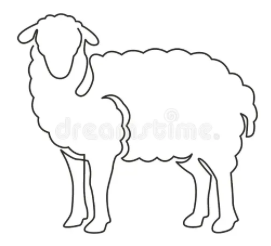
\includegraphics[height=0.6cm]{images/lamb1.png}\ \small Brought into Glory}
\fancyhead[RO]{\small\leftmark\ 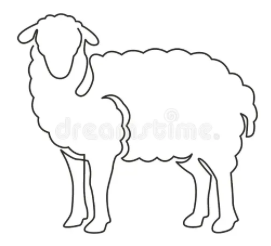
\includegraphics[height=0.6cm]{images/lamb1.png}}
\fancyfoot[LE,RO]{\thepage}
\renewcommand{\headrulewidth}{0pt}

\renewcommand{\chaptermark}[1]{%
  \markboth{Chapter \thechapter\ #1}{}}

\fancypagestyle{plain}{
  \fancyhf{}
  \fancyfoot[LE,RO]{\thepage}
  \renewcommand{\headrulewidth}{0pt}
}

% ---------- Chapters (English) ----------
\renewcommand{\chaptername}{Chapter}
\renewcommand{\thechapter}{\arabic{chapter}}

% ---------- Footnotes ----------
\usepackage{csquotes}
\setlength{\footnotemargin}{0pt}
\renewcommand{\footnotelayout}{\raggedright}

% ---------- Symbols ----------
\usepackage{pifont}
\usepackage{amssymb}
\usepackage{fontawesome5}

% ---------- Chapter style ----------
\titleformat{\chapter}[display]
  {\Huge\bfseries\raggedright}
  {Chapter \thechapter}
  {1cm}
  {\hyphenpenalty=10000\exhyphenpenalty=10000}








\begin{document}

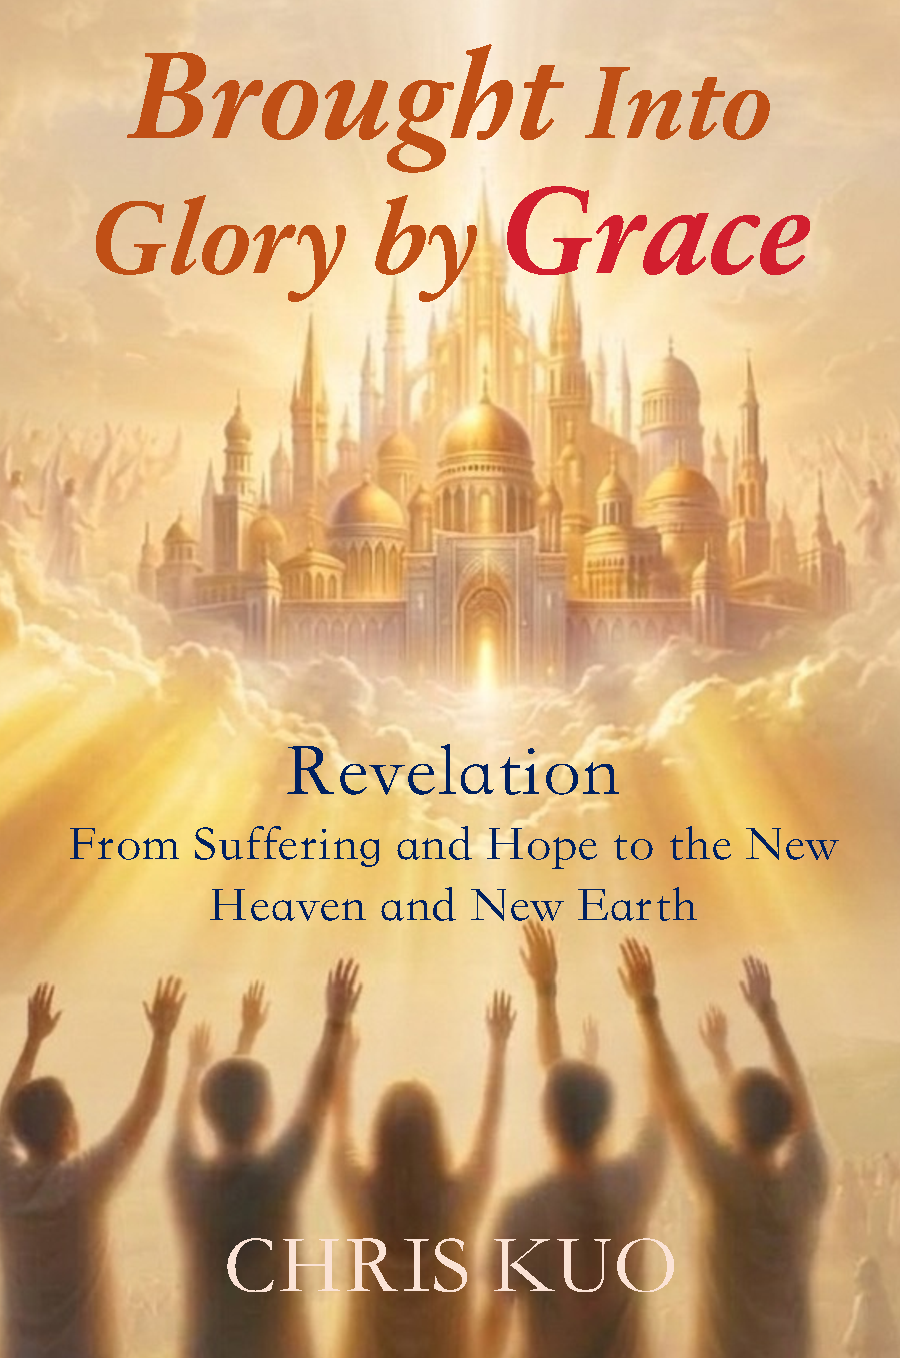
\includepdf[
  pages=1,
  fitpaper=true,
  scale=1
]{cover/English_ebook_6_9.pdf}



% =========================
% Front Matter
% =========================

%\frontmatter
%\pagenumbering{arabic}

% ----- Copyright -----
\clearpage
\thispagestyle{empty}
\vspace*{\fill}
\footnotesize

\noindent
© 2026 Chris Kuo

\vspace{0.5cm}

\noindent 
ISBN: 979-8-9825592-2-7\\
First edition: December, 2026

\vspace{0.5cm}
\noindent All rights reserved. No part of this publication may be reproduced, stored in a retrieval system, or transmitted in any form or by any means, electronic, mechanical, photocopying, recording, scanning, or otherwise, except as permitted under Section 107 or 108 of the 1976 United States Copyright Act, without the prior written permission of the publisher, or in the case of brief quotations embodied in critical reviews and certain other noncommercial uses permitted by copyright law. 

While every effort has been made to ensure the reliability of the information presented in this publication, Innovation Press assumes no responsibility for errors or omissions. However, neither the author nor Innovation Press assumes any liability for damages resulting from the use of the information contained herein. 

The illustrations included in the second edition were created by the author with the assistance of Microsoft Copilot and were subsequently reviewed, edited, and curated for educational purposes.

Email address: ck2869@columbia.edu


\vfill

\noindent The Innovation Press, \\
\noindent Ann Arbor, MI 
\begin{figure}[!htbp]
  
\includegraphics[width=0.20\textwidth]{others/innovation_press.png}% Replace example-image with the filename of your image
\end{figure}
\vfill

% ----- Copyright -----
\clearpage
\thispagestyle{empty}
\vspace*{\fill}
\begin{center}
\large
My dear friend \rule{2cm}{0.4pt}:

\medskip
If you sometimes think of heaven, \\
then this book is for you.
\end{center}
\vspace*{\fill}


% ----- TOC -----
% ----- Front Matter -----
\pagenumbering{roman}

\clearpage
\addcontentsline{toc}{chapter}{The Gospel Revelation Has for You}
\begin{center}
\begin{tcolorbox}[
    width=0.95\textwidth,
    colback=white, %gray!5,
    colframe=gray!70,
    colbacktitle=gray,
    coltitle=white,
    title={\small Did you know that Revelation holds the gospel for you?},
    halign title=center,
    fontupper=\small\setstretch{1.0},
    enhanced,
    boxrule=0.5pt,
    breakable,
    left=3pt,
    right=3pt,
    top=6pt,
    bottom=6pt
]

\textbf{(1) You Were Made by God, and You Are Precious in His Sight}

\hspace{0.5cm} Your life is not an accident. God created all things, and He made you in His own glorious image, giving you a dignity no one can take away. You were made to know Him.
\begin{ScriptureBox}
\item[4:11] You are worthy, our Lord and God, to receive glory and honor and power, for you created all things, and by your will they were created and have their being.
\end{ScriptureBox}

\vspace{0.15cm}
\textbf{(2) Jesus Loves You and Gave His Life to Redeem You}

\hspace{0.5cm} Before Revelation speaks of judgment, it first shows us a Savior. Jesus Christ, the Lamb of God, loves us. He laid down His life and, with His own blood, bought people from every nation and tribe to bring them home to God. That includes you.
\begin{ScriptureBox}
\item[1:5] To him who loves us and has freed us from our sins by his blood.
\item[5:9] Because you were slain, and with your blood you purchased for God persons from every tribe and language and people and nation.
\end{ScriptureBox}

\vspace{0.15cm}
\textbf{(3) Why We Need Him}

\hspace{0.5cm} We need a Redeemer because every one of us has wandered away from God. We often live as though we belong to ourselves, letting good things take the place that belongs to God alone; we cannot even see how poor we have become. One day every life will be laid open before God, and our good deeds cannot wash away our guilt. Yet the Lord does not tell us this to crush us. He tells us because He loves us and longs for us to come back to Him.
\begin{ScriptureBox}
\item[3:17] You say, `I am rich; I have acquired wealth and do not need a thing.' But you do not realize that you are wretched, pitiful, poor, blind and naked.
\item[3:19] Those whom I love I rebuke and discipline. So be earnest and repent.
\item[20:12] The dead were judged according to what they had done as recorded in the books.
\end{ScriptureBox}

\begin{itemize}[leftmargin=2em, labelsep=0.3em]
\item[Q.] \AskItem{Have you sensed that something is missing between you and the God who made you, and that you need His forgiveness?}
\end{itemize}

\vspace{0.15cm}
\textbf{(4) Come to Him Today}

\begin{ScriptureBox}
\item[7:14] They have washed their robes and made them white in the blood of the Lamb.
\item[3:20] Here I am! I stand at the door and knock. If anyone hears my voice and opens the door, I will come in and eat with that person, and they with me.
\item[22:17] The Spirit and the bride say, ``Come!'' And let the one who hears say, ``Come!'' Let the one who is thirsty come; and let the one who wishes take the free gift of the water of life.
\item[21:4] He will wipe every tear from their eyes. There will be no more death or mourning or crying or pain, for the old order of things has passed away.
\end{ScriptureBox}

\hspace{0.5cm} Those who stand before God do so not because they have never sinned, but because they have washed their stained hearts clean in the blood of the Lamb.

\hspace{0.5cm} You do not have to make yourself good enough first. Christ is already knocking at your door. Come just as you are: confess your sins to Him, turn back to Him, and believe that Jesus died and rose again for you. Salvation is His free gift to you.

\vspace{0.15cm}

\begin{itemize}[leftmargin=2em, labelsep=0.3em]
\item[Q.] \AskItem{Will you accept God's gracious invitation today?}
\end{itemize}


If you are willing, you can pray in your own words, or pray the following:

\begin{tcolorbox}[
    width=\linewidth,
    colback=gray!5,
    colframe=gray!70,
    colbacktitle=gray!90,
    coltitle=white,
    title={Prayer},
    center title,
    boxrule=0.5pt,
    breakable,
    left=1pt,
    right=1pt,
    top=1pt,
    bottom=1pt
]
Dear Heavenly Father,

\hspace{0.5cm} Thank You for creating me and loving me. I confess that I have wandered away from You, living for myself and sinning against You. Please forgive my sins.

\hspace{0.5cm} Lord Jesus, I believe that You are the Son of God, that You shed Your blood and gave Your life for me, and that You rose again from the dead.

\hspace{0.5cm} Now I open the door of my heart and receive You as my Savior and the Lord of my life. Please come into my heart, wash me clean with Your precious blood, and make me Your child.

\hspace{0.5cm} May Your Holy Spirit guide me to follow and worship You all my life, until the day I dwell with You in the new heaven and the new earth.

\hspace{0.5cm} In the name of the Lord Jesus Christ I pray. Amen.
\end{tcolorbox}


\end{tcolorbox}
\end{center}


\clearpage
\vspace*{-1.1in}
{
\setstretch{1.2}
\tableofcontents
}

\makeatletter
{%
\vspace*{-0.5cm}
  \renewcommand{\listtablename}{Tables}%
  \setlength{\cftafterlottitleskip}{1em}%
  \setstretch{1.0}%
  \setlength{\cfttabindent}{0pt}   % List of Tables: start at the left margin
  \setlength{\cftbeforetabskip}{0.4em}%
  \let\addvspace\@gobble
  \listoftables
}

\vspace*{0.3cm}
{%
  \renewcommand{\listfigurename}{Figures}%
  \setlength{\cftafterloftitleskip}{1em}%
  \setstretch{1.0}%
 \setlength{\cftfigindent}{0pt}   % List of Figures: start at the left margin
  \setlength{\cftbeforefigskip}{0.4em}%
  \let\addvspace\@gobble
  \let\clearpage\relax
  \listoffigures
}
\makeatother


% Main Matter
%\mainmatter
%\pagenumbering{arabic}

% Main Matter
\clearpage
\pagenumbering{arabic}





\chapter*{Preface}
\addcontentsline{toc}{chapter}{Preface}
\markboth{Preface}{Preface}


\section*{Why Invite You to Read This Book?}

Perhaps you have never heard of Revelation. Or perhaps you know that it is the last book of the Bible, yet wonder whether its message can be trusted. You may read the Scriptures regularly but find Revelation difficult to understand.

If any of these descriptions sound like you, this book was written with you in mind.

If you have not yet encountered the Christian faith, you may assume that Revelation is a book intended only for Christians. But I would like you to know that Revelation is God's own invitation to discover the good news of His gospel. After John wrote this book, it circulated among the churches of Asia Minor. Many early Christians held fast to their faith under pressure and persecution\index{persecution}, some bearing witness to Christ even at the cost of their lives. Their faith rested on the Christ who had truly come into the world.

\section*{Why I Wrote This Book}

There are many films about end-times prophecies, as well as movies and animated productions set against the backdrop of the world's final days. Such stories naturally awaken curiosity about the world portrayed in Revelation. Some people therefore turn to the Bible to discover whether it tells us what will happen at the end of the world. A teenager once told me that this was precisely why he had begun reading the Bible: he wanted to find out whether it described the events of the world's end.

Christians, too, can become preoccupied with questions about how to interpret the dragon\index{dragon}, the beast\index{beast}, the mark, the millennium\index{millennium}, and other prophetic details. My own reading of Revelation underwent a similar turning point. I came to realize that I needed to approach the book anew, not by beginning with each individual event, but by beginning with Jesus Christ.

After all, what are the opening words of Revelation? ``The revelation of Jesus Christ.'' This is a book in which Jesus Himself speaks to us. It reveals that He reigns over history, judges evil, triumphs over Satan\index{Satan} and death, will return, and will make all things new, finally bringing the people He has redeemed\index{redemption} into eternal glory\index{glory}.

I also hope that this book will serve as a resource for Sunday school teachers. For this reason, I have sought to explain the background and message of the biblical text as clearly as possible. My prayer is that whether you are reading for personal devotion, studying Scripture in a small group, or preparing to teach others, this book will help you reflect with others on the Jesus Christ to whom Revelation bears witness.

\section*{Christ, the Lamb, at the Center: How Should We Read Revelation?}\index{Lamb, the}

As you read Revelation, you may find yourself puzzled. Wasn't Jesus a man? How, then, does He become a lamb?

To answer this question, we must learn to read the Bible as a whole.

When Jesus first came into the world, He came as the Lamb\index{Lamb, the} who takes away sin. He willingly endured the cruelest form of execution devised by human hands: crucifixion. This was no accident or helpless surrender. He gave Himself willingly to redeem those held captive by sin. How do we know that He suffered for our transgressions? Some seven hundred years before Jesus came to earth, the prophet Isaiah had already foretold His sacrificial death:

\begin{quote}
``But he was pierced for our transgressions, he was crushed for our iniquities; the punishment that brought us peace was on him, and by his wounds we are healed.''
---Isaiah 53:5 (NIV)
\end{quote}

He was led like a lamb to the slaughter, offering Himself as the sacrifice for our sins.

But did the story end there? No. Revelation carries the story of Jesus forward. He came as the Lamb who was slain\index{Lamb, the!slain}, but now He stands as the victorious Lamb, the conquering\index{overcomers} King who leads the armies of heaven. We recognize Him by His robe, dipped in blood (Revelation 19:13). The One who gave His life is the One who reigns in victory.

Revelation, then, is a story centered on Jesus Christ. He reigns, opens the scroll\index{scroll}, judges evil, defeats Satan\index{Satan}, and brings the people He has redeemed into the glory of the new creation.

How blessed are the countless Christians throughout the ages who have been brought by grace\index{grace} into the glory of God! I believe that you, too, may be among those richly blessed by His grace. My hope is that, after reading this book, you will respond to the Lord's gracious invitation and come to know the One who calls you into His glory.

\section*{About The \textit{by Grace} Series}\index{grace}

This book continues the naming theme of my earlier work, \textit{Caught by Grace}. Together, these titles trace the journey of a person saved by grace: first, caught by God's grace; then, changed by His grace; and finally, brought by His grace into His glory.

The three titles in this series express this journey:

\begin{itemize}
    \item \textit{Caught by Grace}
    \item \textit{Changed by Grace}
    \item \textit{Brought into Glory by Grace }
\end{itemize}

On the cover of this book, the word ``Grace'' appears in red, symbolizing the blood of Jesus Christ through which we are brought into His glory.

Why, then, write the third book, \textit{Brought into Glory by Grace}, first? Because \textbf{knowing the destination helps us understand the purpose of the transformation along the way.} God's salvation in Christ has a glorious end: we will ultimately share in the glory of Christ Himself.

When we know where we are going, we can better understand why God must continue to transform us today. This is the truth Paul sets forth in the golden chain of salvation in Romans 8:

\begin{quote}
``For those God foreknew he also predestined to be conformed to the image of his Son, that he might be the firstborn among many brothers and sisters. And those he predestined, he also called; those he called, he also justified; those he justified, he also glorified.''
---Romans 8:29--30 (NIV)
\end{quote}

From foreknowledge and predestination to calling, justification, and finally glorification, the journey of salvation is not a path we travel by our own strength toward glory. It is God who, by His grace, leads those He has redeemed all the way to that glorious destination.

\section*{Research Background}

The literature on Revelation is vast, and in preparing this introductory guide, I have necessarily had to be selective. In addition to consulting the work of several biblical scholars and commentators, I have drawn on my notes and teaching materials.
As I revisited and reorganized this material, I made many new discoveries and gained fresh insights. 

The following authors and works were particularly important to this book:

\begin{enumerate}
    \item John MacArthur\index{MacArthur, John}\footnote{MacArthur, J. (2007). \textit{Because the Time Is Near: John MacArthur Explains the Book of Revelation}. Moody Publishers.} --- His verse-by-verse exposition and his discussions of Christ's return, sovereign reign, and ultimate victory were valuable resources.

    \item Grant R. Osborne\index{Osborne, Grant R.}\footnote{Osborne, G. R. (2002). \textit{Revelation}. Baker Academic.} --- His examination of different approaches to interpreting Revelation helped me consider its symbols, literary structure, and eschatological themes from multiple perspectives.

    \item G. K. Beale\index{Beale, G. K.}\footnote{Beale, G. K. (1999). \textit{The Book of Revelation: A Commentary on the Greek Text}. Wm. B. Eerdmans Publishing Co.} --- His extensive research into the Old Testament background of Revelation helped me read this book within the larger biblical story and recognize the richness of its Old Testament imagery and theological connections.

    \item Craig R. Koester\index{Koester, Craig R.}\footnote{Koester, C. R. (2014). \textit{Revelation: A New Translation with Introduction and Commentary}. Yale University Press.} --- His work on the historical setting and literary context of Revelation helped me better understand the message this book conveyed to its original readers in the churches of Asia Minor.

    \item Richard Bauckham\footnote{Bauckham, R. (1993). \textit{The Theology of the Book of Revelation}. Cambridge University Press.} --- His theological studies helped me explore the book's central themes more deeply.
\end{enumerate}

These scholars make distinct contributions and offer different interpretations. I have therefore sought, as far as possible, to present the major alternative viewpoints fairly. My purpose is to guide readers through Revelation in an accessible way while keeping its central focus firmly on the victory of Jesus Christ and the ultimate entrance of His people into eternal glory.

\section*{Tables and Timelines}

Revelation contains a wealth of visions, images, and theological themes. To help modern readers grasp this richness, I have organized information into tables and timelines wherever these formats can present it clearly and concisely.

In this way, the main text can remain focused on the sovereignty and victory of Jesus Christ and His ultimate work of making all things new. Where different interpretations of a passage need further explanation, I have addressed them in footnotes or appendices.

\section*{Illustrations in This Book}

Revelation is filled with vivid and powerful images: the dragon\index{dragon}, the beasts, the Lamb, the golden lampstands\index{lampstands}, the trumpets, the seals, the bowls, and the New Jerusalem\index{New Jerusalem}. For modern readers, these visions can sometimes be difficult to picture from words alone. I have therefore included selected illustrations to help readers visualize the scenes and better grasp the message conveyed by the biblical text.

Although conceiving and producing these illustrations required considerable time and effort, I believe that effort is worthwhile if it helps brothers and sisters enter more deeply into the visionary world of Revelation.

Yet illustrations can also shape the reader's imagination, sometimes introducing details that the biblical text itself does not explicitly provide. For this reason, I have sought to keep the illustrations simple, using them primarily as visual aids rather than allowing them to replace the descriptions and explanations of Scripture.\footnote{The illustrations in this book were developed and refined by the author through repeated revisions with Google Gemini, then reviewed, edited, and selected by the author for the final manuscript.}
The illustrations are intended to assist in understanding its figures, scenes, and message, not to serve as an authoritative interpretation of Scripture.

\section*{Closing Reflections}

When I completed the first draft of this book, my heart was filled with awe. I, a sinner saved by grace, had undertaken to write, as best I could, of His glory. The radiant light of His love shone upon me, making my pen race joyfully across the page. Yet before my Creator\index{Creator}, this clumsy pen of mine, so inadequate to express what I longed to say, seemed little more than the startled cry of a crow.

But my Creator\index{Creator} knows. He knows that what I have sought to proclaim through these pages is the glory of the Lord whom I love, worship\index{worship}, and await with longing.

And so, with the apostle John, I close with these words from the final pages of Revelation:

\begin{quote}
``Amen. Come, Lord Jesus.''
---Revelation 22:20 (NIV)
\end{quote}

\vspace{2em}

\begin{flushright}
Your servant in Christ,\\
Chris Kuo\\
Elder, Reformed Church of Newtown\\
Elmhurst, New York
\end{flushright}

\chapter{Behold the Glorious Christ (1:1--1:11)}

What does 'glory' mean to us?

In the four Gospels, we encounter Jesus at His first coming to earth. He came among us in humility. He served others, healed the sick, sought the lost, and ultimately ``gave his life as a ransom for many.''

In many Catholic churches, Jesus is depicted upon the cross. A crown of thorns rests upon His head, and His body bears the wounds of the scourging. This is Jesus, the suffering Servant, the One who endured death for our sake. 

It is difficult to reconcile such an image of humility with what we usually think of as glory.

The apostle Paul tells us that Christ was in very nature God, yet He ``made himself nothing by taking the very nature of a servant'' and humbled Himself in obedience, even to death on a cross (Philippians 2:6--8, NIV).

But the story did not end at the cross.

``Therefore God exalted him to the highest place and gave him the name that is above every name, that at the name of Jesus every knee should bow, in heaven and on earth and under the earth.''
---Philippians 2:9--10  

This is the glorious Christ whom Revelation invites us to behold.

From its very opening, Revelation gives us the voice of the risen and glorified Christ. The One who once walked among us in humility now stands before us in majesty, reigning over history and calling His people to see Him as He truly is.

\begin{ScriptureBox}

\item[1:1] The revelation from Jesus Christ, which God gave him to show his servants what must soon take place. He made it known by sending his angel to his servant John,

\item[1:2] who testifies to everything he saw---that is, the word of God and the testimony of Jesus Christ.

\item[1:3] Blessed is the one who reads aloud the words of this prophecy, and blessed are those who hear it and take to heart what is written in it, because the time is near.

\item[1:4] John, To the seven churches in the province of Asia: Grace and peace to you from him who is, and who was, and who is to come, and from the seven spirits before his throne,

\item[1:5] and from Jesus Christ, who is the faithful witness, the firstborn from the dead, and the ruler of the kings of the earth. To him who loves us and has freed us from our sins by his blood,

\item[1:6] and has made us to be a kingdom and priests to serve his God and Father---to him be glory and power for ever and ever! Amen.

\item[1:7] ``Look, he is coming with the clouds,'' and ``every eye will see him, even those who pierced him''; and all peoples on earth ``will mourn because of him.'' So shall it be! Amen.

\item[1:8] ``I am the Alpha and the Omega,'' says the Lord God, ``who is, and who was, and who is to come, the Almighty.''

\item[1:9] I, John, your brother and companion in the suffering and kingdom and patient endurance that are ours in Jesus, was on the island of Patmos because of the word of God and the testimony of Jesus.

\item[1:10] On the Lord's Day I was in the Spirit, and I heard behind me a loud voice like a trumpet,

\item[1:11] which said: ``Write on a scroll what you see and send it to the seven churches: to Ephesus, Smyrna, Pergamum, Thyatira, Sardis, Philadelphia and Laodicea.''

\end{ScriptureBox}

\section{John Recorded Revelation on the Island of Patmos}

John is traditionally associated with five books of the New Testament: the Gospel of John, 1 John, 2 John, 3 John, and Revelation.

During the reign of the Roman emperor, John was exiled to the island of Patmos because of his Christian faith and his testimony to Jesus Christ. It was there that he received and recorded the visions preserved in Revelation.
The circle in Figure~\ref{fig:turkey-seven-churches} marks the island of Patmos,
and the numbers show the seven churches: \ding{172} Ephesus, \ding{173} Smyrna, \ding{174} Pergamum, \ding{175} Thyatira, \ding{176} Sardis, \ding{177} Philadelphia, and \ding{178} Laodicea. 


\begin{figure}[htbp]
    \centering
    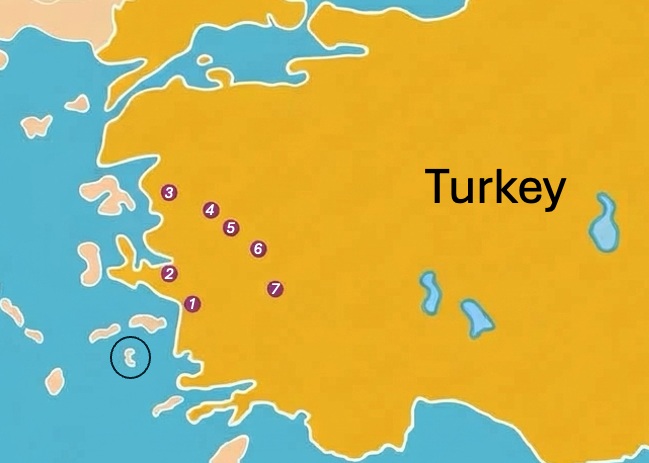
\includegraphics[
        width=0.9\textwidth,
        trim=0 0 0 100,
        clip
    ]{images/turkey}
    \caption{The Seven Churches}
    \label{fig:turkey-seven-churches}
\end{figure}

In such a lonely and troubled place, could the visions John witnessed have been nothing more than hallucinations?

There are good reasons not to dismiss his testimony in this way.

First, John's account does not portray him as someone who had lost consciousness or become detached from what was happening around him. As the visions unfolded, he often knew what he was seeing. He recorded explanations given by angels, asked questions, and received answers. His account presents a witness being shown and instructed, not merely someone recounting a series of bewildering impressions.

Second, Revelation was preserved and transmitted within the early Christian community. In the second century, the church father Irenaeus quoted Revelation repeatedly in his work \textit{Against Heresies}.\footnote{Irenaeus. (1885). \textit{Against Heresies} (A. Roberts \& W. H. Rambaut, Trans.). Christian Literature Publishing. (Original work published ca. 180).} Irenaeus lived relatively close to the apostolic age, and his writings provide important evidence for the early reception of Revelation.

In the fourth century, the church historian Eusebius gathered traditions from the early church in his \textit{Ecclesiastical History}. He recorded traditions concerning John, Patmos, and the period of the emperor Domitian.\footnote{Eusebius. (1890). \textit{Church History} (A. C. McGiffert, Trans.). Christian Literature Company. (Original work published ca. 325).} Eusebius also recorded the tradition that John later returned to Ephesus.\footnote{Eusebius, ca. 325/1885, 3.18.1, 3.20.9.}

Taken together, this early testimony helps establish that Revelation was not a later invention detached from the apostolic church. It was received, preserved, and transmitted as an apostolic witness within the early Christian community.

What, then, is the Christ revealed in this book?

\section{The Glorious Christ}

If the Jesus you know is the suffering Servant, you can be certain that He is also the exalted King.

Colossians 1:15 declares that the Son ``is the image of the invisible God.'' Hebrews 1:3 describes Him as ``the radiance of God's glory and the exact representation of his being''  .

In Revelation 1--3, we encounter one description after another of the glory of Jesus Christ. These descriptions can be brought together in Table~\ref{tab:christ-revelation-1-3}.

\begin{longtable}{p{1.2cm} p{7.8cm}}
\caption{Descriptions of Jesus Christ in Revelation 1--3}
\label{tab:christ-revelation-1-3} \\

\hline
\textbf{Passage} & \textbf{Description of Jesus Christ} \\
\hline
\endfirsthead

\hline
\textbf{Passage} & \textbf{Description of Jesus Christ} \\
\hline
\endhead

\hline
\endfoot

\hline
\endlastfoot

1:5
& The firstborn from the dead. He has conquered death and stands as the beginning of the new creation. \\

3:14
& The ruler of God's creation, supreme over all that has been made. \\

1:8
& The Alpha and the Omega, the beginning and the end. He transcends time and holds history in His sovereign hands. \\

1:13
& One like a son of man, clothed in a robe reaching down to His feet and with a golden sash around His chest. His appearance conveys majesty and evokes the dignity of a royal and priestly figure. \\

1:14
& His head and hair are white like wool, as white as snow. The imagery conveys holiness and majesty and recalls the Ancient of Days in Daniel's vision. \\

1:14; 2:18
& His eyes are like blazing fire. Nothing is hidden from His sight. He searches the human heart and sees the truth about every person and every church. \\

1:15; 2:18
& His feet are like bronze glowing in a furnace. The imagery suggests strength, purity, and the authority to execute righteous judgment. \\

1:15
& His voice is like the sound of rushing waters, conveying overwhelming majesty and authority. \\

1:16; 2:1; 3:1
& He holds the seven stars in His right hand and walks among the seven golden lampstands. He holds the seven stars and the seven spirits of God. These images portray His authority over the churches, His presence among them, and His sovereign rule. \\

1:16; 2:12
& A sharp double-edged sword comes from His mouth. His word exposes error, judges evil, and defeats His enemies. \\

1:16
& His face shines like the sun in all its brilliance, revealing His divine majesty and glory. \\

1:18
& He holds the keys of death and Hades, demonstrating His authority over death and the realm of the dead. \\

3:7
& He holds the key of David. As the rightful King, He opens what no one can shut and shuts what no one can open. \\

3:14
& He is the faithful and true witness, wholly trustworthy in all He reveals and declares. \\

\end{longtable}

\section{The Old Testament Foretold the Glory of Christ}

The glorious Christ John describes bears a striking resemblance to the figures and visions seen by Old Testament prophets centuries earlier.

This is no coincidence. Jewish readers familiar with the Scriptures would recognize in Revelation's portrayal of Christ the glorious King whom the Old Testament had anticipated and promised.

\begin{itemize}
    \item \textbf{Daniel 7:9.} ``As I looked, thrones were set in place, and the Ancient of Days took his seat. His clothing was as white as snow; the hair of his head was white like wool. His throne was flaming with fire, and its wheels were all ablaze.''  

    \item \textbf{Daniel 7:13.} ``In my vision at night I looked, and there before me was one like a son of man, coming with the clouds of heaven.''  

    \item \textbf{Daniel 7:14.} ``He was given authority, glory and sovereign power; all nations and peoples of every language worshiped him. His dominion is an everlasting dominion that will not pass away, and his kingdom is one that will never be destroyed.''  

    \item \textbf{Daniel 10:6.} ``His body was like topaz, his face like lightning, his eyes like flaming torches, his arms and legs like the gleam of burnished bronze, and his voice like the sound of a multitude.''  

    \item \textbf{Ezekiel 43:2.} ``And I saw the glory of the God of Israel coming from the east. His voice was like the roar of rushing waters, and the land was radiant with his glory.''  

    \item \textbf{Isaiah 22:22.} ``I will place on his shoulder the key to the house of David; what he opens no one can shut, and what he shuts no one can open.''  
\end{itemize}

These prophets received visions of divine glory in troubled times. The Lord of glory had not forgotten His servants. Rather, He revealed His majesty to them, becoming their strength and their hope.

If the Jesus in your imagination is only the suffering figure who was rejected, abandoned, and nailed to the cross, you need to remind yourself of the greater truth: He is the image of God, the risen and victorious Lord who reigns in glory.

When we come to know Christ in His glory, we discover a hope that sustains us through present suffering, a strength that upholds us in weakness, and a faithfulness that endures even in darkness. We can remain steadfast because the One who walks among His churches is the One who conquered death and will come again.

\section*{Discussion Questions}

\begin{enumerate}
    \item The same Christ who took the form of a servant, suffered for us, was rejected, and died on the cross now reigns in glory and rules over the kings of the earth. How do these two sides of Jesus help us know Him better?
    
    \item Jesus is the First and the Last, He rose from the dead, and He holds the keys of death and Hades. How does this help us stay faithful in hard times?

    \item If we know that one day we will reign with Christ and serve in the presence of God, how should that hope shape the way we live today as people who belong to Him?
\end{enumerate}
\chapter{Christ Speaks to His Churches (2:1--3:13)}
\normalsize

\section{The World of the Early Church}

The years that John wrote Revelation were among the most powerful in the history of the Roman Empire\index{Roman Empire}. Earthly rulers appeared nearly invincible, their authority reaching across vast territories and their power beyond challenge.

It was in this very age that God established the early Church. Believers came to know the true King, Jesus Christ, and bore witness to Him, even at the cost of their lives.

Emperor worship\index{emperor worship} gradually became part of public life. Religious policies, however, were not entirely uniform across the empire. As long as they were not perceived as threats to public order, many peoples were permitted to retain their traditional religious practices. Judaism, with its long history, enjoyed a degree of religious privilege under Roman rule, allowing Jewish communities to worship\index{worship} the God of their ancestors according to their established laws and customs. 

Christianity initially emerged from this Jewish setting, and in some places Christians were regarded as part of the broader Jewish tradition. As Christianity gradually became more distinct from Judaism, however, the protection afforded by that inherited religious status diminished.\footnote{Beale, G. K. (1999).}

Christians worshiped the one true God and confessed Jesus Christ as Lord. They could not, therefore, worship the emperor as a god. This refusal could expose them to social hostility and official pressure. In some regions, they faced the danger of confiscation of property, exile, imprisonment, or even execution.

\begin{figure}[htbp]
    \centering
    \caption{Timeline of Roman Emperors, AD 1--138}
    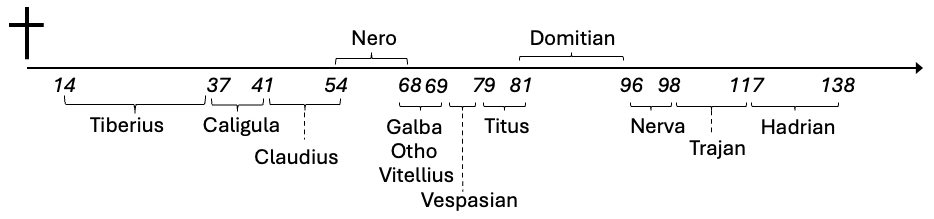
\includegraphics[
    width=1\textwidth,
    trim=0 0 0 0,
    clip]{images/roman_emperors.png}
    \label{fig:roman_emperors}
\end{figure}

I drew a timeline of Roman emperors from AD 1 to 138 in Figure~\ref{fig:roman_emperors}.
Among these emperors, Nero\index{Nero} and Domitian\index{Domitian} are often remembered in historical accounts as tyrants. Both concentrated power in their own hands, suppressed political rivals, and executed opponents, sometimes under charges such as treason. Nero is especially remembered for persecuting Christians after the Great Fire of Rome\index{Rome} in AD 64. Table \ref{table:nero_domitian} highlights the facts.\footnote{As for Domitian, ancient sources describe his suppression of dissent, but scholars continue to debate whether he conducted a large-scale persecution of Christians.}


{
\small
\begin{longtable}{|p{2.5cm}|p{6.5cm}|}
\caption{Nero and Domitian: persecution and rule}
\label{table:nero_domitian} \\
\hline
\textbf{Emperor}\footnote{The portrait of Nero is held by the Glyptothek in Munich; the portrait of Domitian is held by the Louvre in France.}
&
\textbf{Persecution and Rule}
\\
\hline

\centering
Nero

\includegraphics[
    width=\linewidth,
    trim=0 0 0 0,
    keepaspectratio
]{images/nero.jpg}

&
\vspace{-0.3cm}
\begin{itemize}[nosep, leftmargin=10pt]
\item Executed political rivals and members of the Senate.
\item Used legal charges, including treason, to suppress opponents.
\item Ordered the murder of his own mother, Agrippina.
\item Persecuted Christians following the Great Fire of Rome in AD 64.
\item Ruled through fear, violence, and arbitrary power.
\item Those who refused to participate in emperor worship could be accused of atheism or impiety.
\end{itemize}
\\[-0.5cm]
\hline

\centering
Domitian

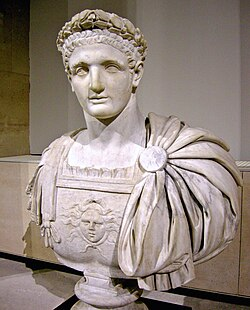
\includegraphics[
    width=\linewidth,
    keepaspectratio
]{images/domitian.jpeg}

&
\vspace{-0.3cm}
\begin{itemize}[nosep, leftmargin=10pt]
\item Executed senators and political opponents.
\item Used legal charges, including treason, to suppress rivals.
\item Confiscated the property of convicted opponents.
\item Was associated with the title ``Lord and God'' (\textit{Dominus et Deus}), which Suetonius says was used in addressing him.\footnote{Suetonius. (1914). \textit{Lives of the Caesars: Volume II} (J. K. Rolfe, Trans.). Harvard University Press.}
\item Those who refused to participate in emperor worship could be accused of atheism or impiety.
\item Ruled through suspicion, informants, and repression.
\end{itemize}
\\
\hline
\end{longtable}
}

Against this backdrop of persecution\index{persecution}, let us turn to the letters Jesus addressed to the seven churches\index{seven churches}. The locations of the seven churches can be seen in Figure~\ref{fig:turkey-seven-churches}.

\normalsize

\subsection{Why These Seven Churches?}\index{seven churches}

A reader's first question may be this: Why these seven churches\index{seven churches}? The New Testament also mentions churches in Rome\index{Rome}, Corinth, Philippi, Colossae, Thessalonica, and many other cities. Why are they not included here?

The seven churches\index{seven churches} in Revelation were not chosen at John's own discretion. Christ commanded him: ``Write on a scroll\index{scroll} what you see and send it to the seven churches'' in Asia.

The number seven appears repeatedly throughout Revelation and often conveys a sense of completeness. These letters, therefore, were not intended only for the seven congregations that first received them. Each letter concludes with the call to hear what the Spirit says to the churches. What Christ says to one congregation is thus also a message to the wider Church.

To help readers enter the world of these early believers, I have designed a series of imagined conversations between brothers in the faith. Through these dialogues, we may almost step into the churches themselves and listen to how their members understood their circumstances before hearing Christ speak to them.

Each of the seven letters contains Christ's commendation, rebuke, command, and promise. For clarity, I have organized His message under four headings: ``Christ's Commendation,'' ``Christ's Rebuke,'' ``Christ's Command,'' and ``Christ's Promise.''

One detail deserves special attention: two churches receive no commendation at all. The word ``None'' is sobering, even painful. If the Lord were to speak directly to our own churches, would we hear His commendation? Or would we, too, be confronted with that heartbreaking word: ``None''?

\section{The Church in Ephesus (2:1--2:7)}\index{Ephesus}

\begin{DialogueBox}
\noindent\faUser\ Brother One: ``Through the years, our brothers have labored for the Lord's name, endured hardship, and refused to turn back when persecution\index{persecution} came. When people taught strange doctrines, we examined their claims. When men called themselves apostles, we did not accept them without testing them. ''

\vspace{0.1cm}

\noindent\faUser\ Brother Two: ``We have indeed done much in the Lord's name. And yet, at times, I remember the days when we first believed. The brothers and sisters loved one another with such fervor. We gathered eagerly to hear the word, to pray, and to break bread together. But I wonder whether the love we once had for the Lord and for one another has quietly grown cold.''
\end{DialogueBox}

\subsection{Geographical Background}

Ephesus\index{Ephesus}, the city in which this church was established, was prosperous and deeply shaped by the worship of idols.

Visitors to the ruins of ancient Ephesus\index{Ephesus} today can still see the remains of its great theater, Harbor Street, Marble Road, marketplaces, library, temples, and fountains. Walking among these surviving stones, we can begin to imagine the city's former splendor as one of the important centers of the Roman Empire\index{Roman Empire}.

The Temple\index{temple} of Artemis was one of the most important symbols of Ephesian identity. Artemis was the Greek name of the goddess whom the Romans called Diana. Worship of Artemis was more than a religious practice; it also sustained related trades and commercial activities. Acts 19:24 tells us that a silversmith named Demetrius made silver shrines of Artemis, bringing considerable business to the craftsmen.

Then Paul and his companions began proclaiming the gospel in Ephesus\index{Ephesus}. Many people abandoned their idols and turned to Christ. As the gospel transformed lives, it also began to affect the social and economic activities built around idol worship.

Demetrius gathered fellow silversmiths and other craftsmen, accusing Paul and his companions of threatening the honor of Artemis and endangering their livelihood. The whole city was thrown into an uproar. A crowd rushed into the theater and, for about two hours, shouted, ``Great is Artemis of the Ephesians!''

Luke, the physician, records the confusion with a touch of understated irony: the assembly was in disorder, some shouting one thing and others another, and most of the people did not even know why they had gathered (Acts 19:28, 32, 34).

Imagine the multitude filling that enormous theater, shouting for two uninterrupted hours. The scene gives us a sense not only of the scale of Ephesus\index{Ephesus} but also of the intensity of its religious devotion and the central place idol worship occupied in civic life.

It was in this prosperous, influential city, so deeply entangled with the worship of idols, that Christ established His Church.


The church in Ephesus\index{Ephesus} was prominent among all the early churches.
Paul's letter to the Ephesians opens with a magnificent declaration of God's predestination: God chose His people in Christ before the creation of the world (Ephesians 1:4). Paul then unfolds the great mystery God has accomplished in Christ.

That \textit{mystery} is the Church: through the gospel, Gentiles are fellow heirs, members of the same body, and sharers together in the promise in Christ Jesus (Ephesians 3:6).\footnote{The church is called a mystery, one not revealed to the Old Testament saints. Also, see Figure \ref{fig:valley}
in Appendix~\thechapter~ ``How Long Is the Great Tribulation?''}
Paul also prays that Christ may dwell in their hearts through faith, that they may be rooted and established in love, and that together with all the saints they may grasp how wide and long and high and deep is the love of Christ (Ephesians 3:17--18).

\subsection{Christ's Commendation}

\begin{ScriptureBox2}{How does Christ introduce Himself in 2:1? Underline everything He knows and commends about the church.}
% Insert the NIV text of Revelation 2:1--3 here.
\item[2:1] Christ is presented as the One who holds the seven stars in His right hand and walks among the seven golden lampstands.

\item[2:2] He knows the church's deeds, hard work, perseverance, intolerance of wickedness, and careful testing of those who claim to be apostles but are not.

\item[2:3] He commends the believers for enduring hardship for His name and not growing weary.
\end{ScriptureBox2}

These were believers whose faith was expressed through action. They labored for the Lord, endured hardship, guarded the truth, and learned to distinguish truth from error.

When Paul took leave of them, the elders of the Ephesian church wept openly. What grieved them most was his declaration that they would never see his face again (Acts 20:38).

Paul had also solemnly warned them to remain alert, because savage wolves would come among them and would not spare the flock (Acts 20:29). The Ephesian believers had truth, diligence, perseverance, and love. They had much for which to be commended.

\subsection{Christ's Rebuke}

\begin{ScriptureBox2}{What does Christ hold against the church?}
% Insert the NIV text of Revelation 2:4 here.
\item[2:4] Christ rebukes the church because it has forsaken the love it had at first.
\end{ScriptureBox2}

Yet some thirty years after the Church's earliest days, Christ spoke through John and declared that the Ephesians had forsaken their first love.

By this time, the congregation may have included believers of the second or even third generation. Sound teaching remained. The church continued to serve, and its members were still known for their perseverance. From a human perspective, it might have appeared to be a model congregation.

Yet something was quietly slipping away: the love that had marked its beginning.

This is what makes the Ephesian church so searching an example for us. A church may stand firmly for truth, labor tirelessly for the Lord, and endure hardship without surrendering. And yet, almost without noticing, it may lose the love that once gave life and warmth to all its work.

\subsection{Christ's Command}

\begin{ScriptureBox2}{Circle the three things Christ commands the church to do in 2:5. What will happen if they do not repent?}
% Insert the NIV text of Revelation 2:5--6 here.
\item[2:5] Christ calls the church to remember how far it has fallen, repent, and do the things it did at first. He warns that, without repentance, He will remove its lampstand from its place.

\item[2:6] He commends the church for hating the practices of the Nicolaitans, which He also hates.
\end{ScriptureBox2}

How can love that has grown cold be restored? The answer is \textbf{repentance\index{repentance}.}

Repentance awakens a heart that has grown indifferent and rekindles a love that has faded. However far we may have wandered, grace\index{grace} can still turn us around and renew us in the Lord.

Repentance is more than sorrow over past failures. It is a renewed turning toward Christ, a return to the life of loving Him and following Him as we did at the beginning.

We need to repent daily. As the Lord Jesus taught His disciples, we must take up our cross daily and follow Him (Luke 9:23).

It is important to notice that Christ's rebuke does not mean the Ephesian church had compromised the truth. On the contrary, the believers continued to hate the practices of the Nicolaitans\index{Nicolaitans}, and Christ commended them for this. We cannot identify with certainty the precise background or teaching of the Nicolaitans.\footnote{MacArthur, J. (2007).} Nevertheless, their practices represented teachings and behaviors that Christ condemned.

\subsection{Christ's Promise}

\begin{ScriptureBox2}{What does Christ promise to the one who is victorious, and where is it found?}
% Insert the NIV text of Revelation 2:7 here.
\item[2:7] The Spirit calls everyone who has ears to hear what He says to the churches. To the one who is victorious, Christ promises the right to eat from the tree of life in God's paradise.
\end{ScriptureBox2}

The tree of life\index{tree of life} immediately brings us back to Genesis 2--3, while the paradise promised here anticipates Revelation 22:1--5.

From Genesis to Revelation, we see the unfolding of one great story: humanity loses Eden\index{Eden}, redemption\index{redemption} is accomplished through Christ, the victorious enter God's paradise, and God's people finally dwell with Him in the new heaven and new earth\index{new heaven and new earth}.

Christ does not merely call His Church to remain faithful on earth. He will ultimately bring His people into glory\index{glory}.

The struggles, repentance\index{repentance}, endurance, and faithfulness of the Church today are not the end of the story. The story reaches its fulfillment in the eternal presence of God. Christ's promise to Ephesus\index{Ephesus} therefore speaks both to the church's present condition and to the glory toward which He is leading His people.

\section{The Church in Smyrna (2:8--2:11)}\index{Smyrna}

\begin{DialogueBox}
\noindent\faUser\ Brother One: ``We in Smyrna\index{Smyrna} are afflicted and poor by the standards of this world. Some have been slandered because of their faith in Christ. Some of our brothers have already given their lives for the Lord's name. And yet, we still gather to worship Him. If we can remain faithful to Christ, what does earthly poverty matter?''

\vspace{0.1cm}

\noindent\faUser\ Brother Two: ``In the eyes of the world, we may possess almost nothing. But there is one thing we must never surrender: our faithfulness to the Lord. The suffering ahead may be greater than anything we have yet endured. But we belong to Christ. We must hold fast to Him to the end.''
\end{DialogueBox}

\subsection{Geographical Background}

Smyrna\index{Smyrna} is modern-day Izmir, Turkey's third-largest city and an important port on the Aegean coast. Traces of its long history remain visible today, including the ancient agora, Roman-era colonnades, public buildings, and other urban structures.

In Roman times, Smyrna\index{Smyrna} was known for its loyalty to Rome\index{Rome}. As early as approximately 195 BC, the city established a temple\index{temple} dedicated to Roma, the personification of Rome, as a public expression of its allegiance. Later, in AD 26, Smyrna competed with other cities of Asia and won permission to build a temple honoring Emperor Tiberius, Livia, and the Roman Senate.

Against this background, Christians who refused to participate in emperor worship\index{emperor worship} could be viewed as refusing to demonstrate loyalty to Rome\index{Rome}. For the believers in Smyrna\index{Smyrna}, confessing with their hearts and mouths that Jesus is Lord was therefore no trivial matter. It could become a question of livelihood, freedom, and even life itself.

This setting helps us understand how precious Christ's commendation of the church in Smyrna\index{Smyrna} truly was.

\subsection{Christ's Commendation}

\begin{ScriptureBox2}{How does Christ describe Himself in 2:8? What does He know about the church, and how does He see its poverty?}
% Insert the NIV text of Revelation 2:8--9 here.
\item[2:8] Christ identifies Himself as the First and the Last, who died and came to life again.

\item[2:9] He knows the church's affliction and poverty, yet declares it spiritually rich. He also knows the slander spoken by those who claim to be Jews but are described as a synagogue of Satan.
\end{ScriptureBox2}

The church in Smyrna\index{Smyrna} became known for its steadfast faithfulness, even unto death.

Around AD 155--160, Polycarp served as bishop of Smyrna\index{Smyrna}. According to early Christian tradition, he had been acquainted with the apostle John. Polycarp was arrested and brought before the authorities. When ordered to deny Christ, he reportedly answered, ``For eighty-six years I have served him, and he has done me no wrong. How can I blaspheme my King who saved me?''\footnote{\textit{Martyrdom of Polycarp}. (1885). (A. Roberts \& J. Donaldson, Trans.). Christian Literature Publishing. (Original work published ca. 155).}

His martyrdom\index{martyrs} became one of the best-known testimonies of faith in early Christianity.

Smyrna\index{Smyrna} was a city celebrated for its loyalty to Rome\index{Rome}. Yet within that city, Christ had established a people whose ultimate allegiance belonged to Him alone.

\subsection{Christ's Rebuke}

None.

\subsection{Christ's Command}

\begin{ScriptureBox2}{What are the believers told not to fear, and how long will their testing last? What are they commanded to do?}
% Insert the NIV text of Revelation 2:10a here.
\item[2:10a] Christ tells the believers not to fear the suffering ahead. Some will be imprisoned and tested, and they will face tribulation for a limited period. He commands them to remain faithful, even to the point of death.
\end{ScriptureBox2}

The reference to ten days suggests a period that is limited rather than endless. The suffering may be severe, but it does not continue without limit, nor does it escape the sovereign rule of God.

\subsection{Christ's Promise}

\begin{ScriptureBox2}{What two things does Christ promise to the one who is victorious?}
% Insert the NIV text of Revelation 2:10b--11 here.
\item[2:10b] Christ promises the crown of life.

\item[2:11] The one who is victorious will not be hurt by the second death.
\end{ScriptureBox2}

The ``second death\index{second death}'' refers to the final judgment\index{judgment} and eternal punishment (Revelation 20:14).

Victory does not mean that believers earn salvation through their own courage or perseverance. Rather, it describes the faithfulness of those who belong to Christ and continue to hold fast to Him through suffering, sustained by His grace.

For the church in Smyrna\index{Smyrna}, this promise was especially precious. Some believers might be killed because they refused to deny Christ. Yet physical death could not undo the eternal life He had given them.

The One who died and came to life again had already conquered\index{overcomers} death. Those who belong to Him will not suffer the second death\index{second death}. They may lose their earthly lives, but they will never lose the eternal life Christ has promised.

\section{The Church in Pergamum (2:12--2:17)}\index{Pergamum}

\begin{DialogueBox}
\noindent\faUser\ Brother One: ``What a prosperous city Pergamum\index{Pergamum} is, with its many temples and its constant stream of sacrifices. Yet the people here invite us to their banquets, where sacrifices are offered to idols. We cannot always refuse such invitations without consequence. Perhaps we can hold fast to our faith while making a few small concessions elsewhere.''

\vspace{0.1cm}

\noindent\faUser\ Brother Two: ``I have thought the same way. Some brothers say that, as long as we continue to trust Christ in our hearts, it should be harmless to attend these feasts from time to time and eat food sacrificed to idols. But lately my conscience has grown troubled. We were called to turn from idols and come to the Lord. If we keep yielding, little by little, are we preserving our lives—or slowly abandoning the way of Christ?''
\end{DialogueBox}

\subsection{Geographical Background}

Pergamum\index{Pergamum}, known today as Bergama, lies in western Turkey, in Izmir Province. Its ancient ruins are now recognized as a UNESCO World Heritage Site.

Visitors can explore the city's acropolis, perched high on a hill, where the remains of an ancient theater, the Temple\index{temple} of Athena, a library, the altar\index{altar} of Zeus, and a temple associated with the Roman emperor Trajan can be seen. The nearby Asclepion was a celebrated center of ancient medicine and healing, and remains one of the region's most important archaeological sites.

Pergamum\index{Pergamum} was also famous for its library and for parchment, the writing material whose name is derived from the city's own name. It was an important center of learning in the ancient world. Under Roman rule, it became a major city in the province of Asia and an important center of imperial cult\index{emperor worship} activity.

\begin{figure}[htbp]
    \centering
    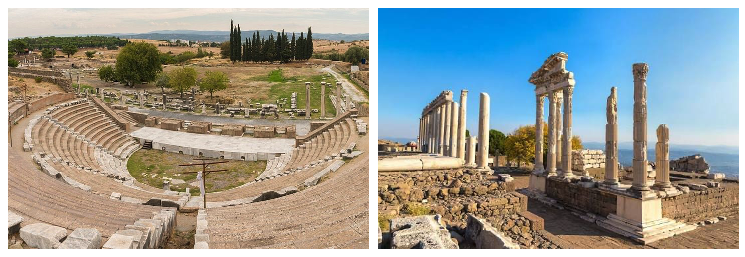
\includegraphics[
    width=1\textwidth,
    trim=0 0 0 0,
    clip]{images/pergamum3.png}
    \caption{The ancient theater and remains associated with the Altar of Zeus at Pergamum}
    \label{fig:pergamum3}
\end{figure}

\subsection{Christ's Commendation}

\begin{ScriptureBox2}{How does Christ introduce Himself in 2:12? Where do these believers live, and what did they do even when Antipas was killed?}
% Insert the NIV text of Revelation 2:12--13 here.
\item[2:12] Christ introduces Himself as the One who has the sharp, double-edged sword.

\item[2:13] He knows where the believers live, in a place described as Satan's throne. Even when His faithful witness Antipas was killed there, the church held firmly to Christ's name and did not renounce its faith.
\end{ScriptureBox2}

Pergamum\index{Pergamum} was not merely a center of culture and learning. It was also a city steeped in religious activity and imperial worship. This background helps explain the force of Christ's description of it as the place ``where Satan\index{Satan} has his throne\index{throne of God}'' (Revelation 2:13).

\subsection{Christ's Rebuke}

\begin{ScriptureBox2}{Whose teachings do some in the church hold to? Underline what Balaam led Israel into.}
% Insert the NIV text of Revelation 2:14--15 here.
\item[2:14] Christ rebukes the church because some hold to the teaching of Balaam, who taught Balak to entice Israel into eating food sacrificed to idols and committing sexual immorality.

\item[2:15] Some also hold to the teaching of the Nicolaitans.
\end{ScriptureBox2}

Numbers 25 describes how Israel\index{Israel} was led into sexual immorality with Moabite women and drawn into idol worship. The episode became a warning about the danger of abandoning faithfulness to God under the influence of surrounding peoples.

Israel had once faced the temptation to compromise in a pagan environment. The church in Pergamum\index{Pergamum} was now confronting a similar danger.

The problem was not new. Israel had faced it in the wilderness, and now the Church was in danger of repeating the same story.

In our own day, this may take the form of teaching and discipleship that encourage compromise: the suggestion that we can retain the language of faith while gradually accommodating practices that draw us away from Christ. Such teaching calls for careful discernment.

\subsection{Christ's Command}

\begin{ScriptureBox2}{What does Christ command, and what will He do if the church does not obey?}
% Insert the NIV text of Revelation 2:16 here.
\item[2:16] Christ commands the church to repent. Otherwise, He will come and fight against those who persist in error with the sword of His mouth.
\end{ScriptureBox2}

As discussed in Table~\ref{tab:christ-revelation-1-3} in Chapter 1, the sword from Christ's mouth represents His authority to judge falsehood and error by His word. Here, He calls the church to turn away from corrupt teaching and conduct and to renew its allegiance to Him.

\subsection{Christ's Promise}

\begin{ScriptureBox2}{What two gifts does Christ promise to the one who is victorious, and what is written on the stone?}
% Insert the NIV text of Revelation 2:17 here.
\item[2:17] The one who is victorious will receive hidden manna and a white stone bearing a new name, known only to the one who receives it.
\end{ScriptureBox2}

Manna first calls to mind the food God provided for Israel\index{Israel} in the wilderness (Exodus 16:15). In a city crowded with pagan worship and hostile pressures, Christ promises His victorious people a different kind of nourishment. Their true sustenance will not come from compromising with idols, but from Christ Himself.

The white stone is often understood in light of Roman customs. In some ancient settings, a white token could signify a favorable verdict, recognition, or admission to a special gathering. One proposed interpretation connects it with athletic victory: a victor might receive a token bearing his name that granted entry to a celebratory banquet.\footnote{MacArthur, J. (2007).} Although the precise background remains uncertain, the image clearly conveys welcome and honor bestowed upon the recipient.

In Scripture, a new name often signifies a renewed identity and a new relationship with God. Christ's promise therefore points to the deeper nourishment and lasting identity He gives to those who remain faithful to Him.

\section{The Church in Thyatira (2:18--2:29)}\index{Thyatira}

\begin{DialogueBox}
\noindent\faUser\ Brother One: ``Our brothers and sisters in Thyatira\index{Thyatira} labor diligently. We love one another, and our faith and perseverance have grown. The charitable work we have recently begun is flourishing, and we are finding new ways to serve our neighbors through the city's trades and associations. If we remain loyal to the Lord while living peaceably with those around us, surely we can bear a good witness here.''

\vspace{0.1cm}

\noindent\faUser\ Brother Two: ``I hope that is so. Yet some things trouble my heart. At the gatherings organized by the trade associations, sacrifices to idols are often offered. And our own church has even welcomed a woman who calls herself a prophet, Jezebel\index{Jezebel}, to teach us. She says that believers may participate in eating food sacrificed to idols.''
\end{DialogueBox}

\subsection{Geographical Background}

Thyatira\index{Thyatira}, also spelled Thyateira, is located in the area of modern Akhisar in western Turkey. It was not especially renowned for monumental political power or for being a major religious center. Instead, it was known for commerce and skilled craftsmanship.

Archaeological evidence points to numerous trade associations, or guilds, in Thyatira\index{Thyatira}, including those of wool workers, dyers, linen workers, leatherworkers, and metalworkers. Lydia, mentioned in Acts 16:14, was a seller of purple cloth from Thyatira. She met Paul in Philippi and later became a Christian.

These guilds were more than professional associations. They also served as social networks and could be closely connected with sacrifices to local deities and religious banquets. Participation in guild life could therefore place Christians under pressure to join practices incompatible with their faith.

Thyatira\index{Thyatira} was known for its metalworking traditions. The description of Christ's feet as being like glowing bronze may have resonated with a community familiar with fine metalwork. The precise alloy intended by the original term is uncertain, but the image conveys the brilliance, strength, and purity of refined metal.\footnote{Osborne, G. R. (2002).}

\subsection{Christ's Commendation}

\begin{ScriptureBox2}{Circle how Christ describes His eyes and feet. Underline the five things He commends, and notice how the church's recent works compare with its first.}
% Insert the NIV text of Revelation 2:18--19 here.
\item[2:18] Christ is introduced as the Son of God, whose eyes are like blazing fire and whose feet are like burnished bronze.

\item[2:19] He commends the church's deeds, love, faith, service, and perseverance, noting that its more recent works are greater than those it did at first.
\end{ScriptureBox2}

\subsection{Christ's Rebuke}

\begin{ScriptureBox2}{What does Christ hold against the church? What has He given Jezebel, and what does He say all the churches will know?}
% Insert the NIV text of Revelation 2:20--23 here.
\item[2:20] Christ rebukes the church for tolerating the woman called Jezebel, who teaches and misleads His servants into sexual immorality and eating food sacrificed to idols.

\item[2:21] He has given her time to repent, but she is unwilling to turn from her immorality.

\item[2:22] He warns of judgment upon her and those who persist in following her.

\item[2:23] He will strike her followers, so that all the churches will know that He searches hearts and minds and repays each person according to their deeds.
\end{ScriptureBox2}

Jezebel\index{Jezebel} was the foreign wife of Ahab, king of the northern kingdom of Israel\index{Israel}. She promoted the worship of Baal, persecuted\index{persecution} the prophets of the Lord, and became a lasting biblical symbol of idolatry and wickedness (1 Kings 17--21).

By calling a contemporary figure in the church ``Jezebel\index{Jezebel},'' John deliberately invokes this Old Testament history to help his readers recognize the nature of the present danger.

The references to sexual immorality and eating food sacrificed to idols include actual participation in pagan worship and its associated social banquets. In the Old Testament, sexual immorality also frequently serves as a metaphor for Israel's unfaithfulness to the Lord through idolatry.

The central issue, therefore, is whether the Church remains faithful to Christ or compromises its allegiance in order to accommodate the surrounding culture, religion, and centers of power.

\subsection{Christ's Command}

\begin{ScriptureBox2}{To whom is Christ speaking in 2:24? What must they do until He comes?}
% Insert the NIV text of Revelation 2:24--25 here.
\item[2:24] Christ addresses those who have not accepted this teaching or learned what its followers call the deep secrets of Satan. He places no additional burden upon them.

\item[2:25] They must hold fast to what they have until He comes.
\end{ScriptureBox2}

The expression ``the deep secrets of Satan\index{Satan}'' has been interpreted in at least two ways.\footnote{Osborne, G. R. (2002); Beale, G. K. (1999).}

\begin{enumerate}
\item \textbf{An ironic expression.} Christ may be speaking sarcastically about the claims of Jezebel\index{Jezebel} and her followers. They may have boasted of their knowledge of the deep things of God, echoing language such as that found in 1 Corinthians 2:10, while in reality leading believers into spiritual danger.

\item \textbf{A more literal interpretation.} Jezebel\index{Jezebel} may have been teaching principles resembling early forms of Gnostic thought.\footnote{Gnostic thought, in its various forms, often distinguished between the material world and the spiritual realm and emphasized hidden knowledge (\textit{gnosis}) as a means of attaining spiritual insight or salvation. The early Christian writings, including the letters of John, oppose teachings that distort the truth about Christ and the nature of salvation. See \textit{Caught by Grace}, Chapter 7, ``On Gnosticism.''} Under this interpretation, believers may have been encouraged to experience the supposed ``depths'' of Satan\index{Satan}, perhaps through participation in pagan practices, in the belief that such experiences would enable them to overcome\index{overcomers} evil.
\end{enumerate}

The first interpretation appears more likely, particularly because of its possible connection with Revelation 2:9, where those opposing the church are described as a ``synagogue of Satan\index{synagogue of Satan}.'' Nevertheless, both interpretations raise questions about claims to possess special spiritual knowledge.

In simple terms, Gnostic thought refers to a range of ideas that emphasized special or hidden knowledge as a means of discovering divine truth and escaping the limitations of the material world. Under the first interpretation, the expression ``deep things of God'' may be a mocking reference to the esoteric knowledge sought by early Gnostic teachers. Under the second, it may involve people who believed that possessing special knowledge allowed them to engage in sinful behavior without spiritual consequences. Such an attitude resembles the kind of moral presumption opposed in 1 John 1:8--10 and 3:9.

Whatever the precise historical background, Christ's command is unmistakable: the believers must hold fast to what they have received and refuse to compromise their faith.

\subsection{Christ's Promise}

\begin{ScriptureBox2}{What does Christ promise to the one who is victorious? Circle the image of authority in 2:27 and the gift in 2:28.}
% Insert the NIV text of Revelation 2:26--29 here.
\item[2:26] Christ promises authority over the nations to those who are victorious and continue to do His will to the end.

\item[2:27] They will share in His authority, described through the imagery of an iron scepter and shattered pottery.

\item[2:28] He promises to give them the morning star.

\item[2:29] The Spirit calls everyone who has ears to hear what He says to the churches.
\end{ScriptureBox2}

In the context of this letter, victory means remaining faithful to Christ's commands in the face of Jezebel\index{Jezebel}'s teaching, idolatry, and the temptation to compromise.

The image of the iron scepter comes from Psalm 2:8--9, where the Lord grants the nations to His anointed King and speaks of ruling them with an iron scepter. This does not mean that believers become another Christ. Rather, the authority Christ receives from the Father is shared with those who belong to Him. The victorious will reign with Christ.

The Greek verb translated ``rule'' can also carry the sense of shepherding or tending. The image therefore need not suggest nothing more than destructive force; it can also convey the authority of a king who governs under God's sovereign purpose.

The morning star\index{morning star} becomes especially significant later in Revelation, when Christ identifies Himself as ``the bright Morning Star'' (Revelation 22:16). The promise to give the morning star thus points ultimately to Christ Himself. The greatest reward is not merely authority or honor. It is Christ Himself, given to His victorious people.

The church in Thyatira\index{Thyatira} teaches us why the Church must reject the teaching represented by Jezebel\index{Jezebel}. The Lamb\index{Lamb, the} has purchased His people with His own blood and will lead them into glory. Because the Lamb alone is worthy of worship, the Church must not divide its allegiance with idols. It must remain faithful to Christ until He brings His people into His glorious presence.

\section{The Church in Sardis (3:1--3:6)}\index{Sardis}

\begin{DialogueBox}
\noindent\faUser\ Brother One: ``Our church in Sardis\index{Sardis} has a good reputation. Many gather whenever we meet, and people throughout the city know that we belong to Christ. When I see such enthusiasm, I cannot help thinking that we must have accomplished much for the Lord, and that He must surely be with us.''

\vspace{0.1cm}

\noindent\faUser\ Brother Two: ``From the outside, it certainly appears so. Yet a question keeps troubling me: is our inner life as healthy as our outward appearance? Have our prayers before the Lord, our mutual encouragement, and our repentance\index{repentance} from sin grown weak? People say that we are alive. But what do we look like in the eyes of the Lord?''
\end{DialogueBox}

\subsection{Geographical Background}

Sardis\index{Sardis} lay approximately thirty to forty miles southeast of Thyatira\index{Thyatira}. Established around 1200 BC, it was one of the ancient world's oldest cities and later became the wealthy and powerful capital of the Lydian kingdom.

Through commerce and trade, Sardis\index{Sardis} accumulated great wealth. It is also associated with some of the earliest coinage in gold and silver.

Sardis\index{Sardis} had once been a formidable military stronghold and was difficult to conquer\index{overcomers}. One of its most notable early rulers was Gyges, who reigned in the seventh century BC and helped establish the city's wealth and influence. His successor, Croesus, became so renowned for his riches and power that he believed he could challenge Cyrus, king of Persia.

In the centuries that followed, however, Sardis\index{Sardis} suffered repeated military reversals, including defeats that exposed weaknesses in its defenses. It gradually lost the political and military prominence it had once enjoyed. Although the city retained a measure of wealth and commercial activity, its former glory as the capital of a powerful kingdom had faded.

By the first century AD, Sardis\index{Sardis} had become, in many respects, a city living in the shadow of its past. It still possessed the wealth, culture, and reputation inherited from its former greatness, but it was no longer the mighty political and military center it had once been.

Sardis\index{Sardis} also had a substantial Jewish community, with a history that may reach back to the fifth or fourth century BC. This community played a meaningful role in the city's life and reflected the long-standing interaction of different cultural and religious groups there.\footnote{Osborne, G. R. (2002).}

\subsection{Christ's Commendation}

None.

\subsection{Christ's Rebuke}

\begin{ScriptureBox2}{What does Christ hold? What reputation does the church have, and what is its true condition?}
% Insert the NIV text of Revelation 3:1 here.
\item[3:1] Christ, who holds the seven spirits of God and the seven stars, declares that although the church has a reputation for being alive, it is dead.
\end{ScriptureBox2}

The phrase ``you have a reputation of being alive'' points to the church's public standing. In the eyes of others, Sardis\index{Sardis} appeared to be a thriving congregation. Christ, however, exposes its inward condition: its spiritual life has withered.

There is a striking contrast with the city's own history. Sardis\index{Sardis} had once enjoyed a glorious reputation, only to decline gradually while retaining the outward signs of former greatness. This parallel is illuminating, though we should not assume that John called the church dead simply because of the city's history. His judgment rests on Christ's knowledge of the church itself.

\subsection{Christ's Command}

\begin{ScriptureBox2}{Circle every command Christ gives in 3:2--3. What will happen if the church does not wake up?}
% Insert the NIV text of Revelation 3:2--3 here.
\item[3:2] Christ commands the church to wake up and strengthen what remains and is about to die, for its deeds have not been found complete before God.

\item[3:3] He calls them to remember what they received and heard, keep it, and repent. If they do not wake up, He will come like a thief, at an hour they do not expect.
\end{ScriptureBox2}

The church in Sardis\index{Sardis} needed to wake up, strengthen what remained, remember, obey, and repent\index{repentance}.

Outwardly, the congregation still existed. Inwardly, however, its spiritual life was fading. Yet something remained. Christ's command was therefore not simply a declaration of condemnation; it was a call to preserve what was left and restore it to strength.

This was a summons to turn back from the brink of spiritual death.

\subsection{Christ's Promise}

\begin{ScriptureBox2}{Who in Sardis has not soiled their clothes? Underline the three promises in 3:5.}
% Insert the NIV text of Revelation 3:4--6 here.
\item[3:4] A few in Sardis have not soiled their clothes. They will walk with Christ, dressed in white, for they are worthy.

\item[3:5] Those who are victorious will be dressed in white. Christ will never blot out their names from the book of life but will acknowledge them before His Father and His angels.

\item[3:6] The Spirit calls everyone who has ears to hear what He says to the churches.
\end{ScriptureBox2}

\section{The Church in Philadelphia (3:7--3:13)}\index{Philadelphia}

\begin{DialogueBox}
\noindent\faUser\ Brother One: ``We in Philadelphia\index{Philadelphia} are a small church, and our strength is slight. Compared with other congregations, we may seem insignificant. Yet we must hold fast to the Lord's word and never deny His name. Our trials are many, and there is little we can accomplish by our own strength. But if the Lord grants us even a little strength, we must use it faithfully and remain steadfast in His way.''

\vspace{0.1cm}

\noindent\faUser\ Brother Two: ``Yes. We have nothing of our own in which to boast. We seek no praise from people; we desire only to be faithful before the Lord. If He opens a door before us, then we will do all we can through the strength He provides.''
\end{DialogueBox}

\subsection{Geographical Background}

Philadelphia\index{Philadelphia}, known today as Alaşehir in Turkey, lay about thirty miles southeast of Sardis\index{Sardis}. Situated along an important trade route, it was sometimes described as a gateway to the East. Of the seven cities, it was among the latest to be established, probably after 189 BC.

The city's founding is associated with Attalus II Philadelphus, brother of Eumenes II, king of Pergamum\index{Pergamum}. Attalus was known for his deep affection and loyalty toward his brother. His epithet, ``Philadelphus,'' means ``brother-loving,'' and the city came to bear a name associated with brotherly love.

Like Sardis\index{Sardis}, Philadelphia\index{Philadelphia} lay in a seismically active region and was frequently shaken by earthquakes\index{earthquake}. Volcanic activity had also enriched the surrounding soil, making it particularly suitable for vineyards. Viticulture therefore became an important part of the local economy.

Frequent earthquakes nevertheless made life difficult. The great earthquake of AD 17, which devastated Sardis\index{Sardis}, also caused extensive destruction in Philadelphia\index{Philadelphia}. Walls developed cracks, buildings were unsafe, and the possibility of another earthquake shaped everyday life and long-term planning.

Because of the destruction caused by the earthquake of AD 17, the Roman emperor exempted Philadelphia\index{Philadelphia} from tribute for five years, allowing the city to recover economically and rebuild.

Another event, during Domitian\index{Domitian}'s reign, may have dealt a serious blow to Philadelphia\index{Philadelphia} around AD 92. Ancient evidence and later interpretations associate this period with pressure to reduce vineyards and expand grain production, possibly to supply the Roman army or in response to food shortages. The exact details and scope of such an order remain uncertain. Nevertheless, restrictions on vineyards would have been economically damaging: grain was less profitable than wine, and the local volcanic soil was not especially suited to grain cultivation. Because vineyards took years to mature, such restrictions would have threatened the livelihoods of local growers and caused widespread resentment in the province of Asia.\footnote{Osborne, G. R. (2002).}

\subsection{Christ's Commendation}

\begin{ScriptureBox2}{What does Christ hold, and what can He open and shut? Underline what He says about the church's strength and faithfulness.}
% Insert the NIV text of Revelation 3:7--9 here.
\item[3:7] Christ is described as holy and true, the One who holds the key of David. What He opens no one can shut, and what He shuts no one can open.

\item[3:8] He knows the church's deeds and its little strength. The believers have kept His word and have not denied His name. He has placed before them an open door that no one can shut.

\item[3:9] Christ promises to make those who oppose the church recognize that He has loved His people.
\end{ScriptureBox2}

The phrase ``who holds the key of David'' directly echoes Isaiah 22:22, where the key of the house of David is placed upon the shoulder of the appointed steward: what he opens no one can shut, and what he shuts no one can open.

The emphasis is on the authority of the One who holds the key. It is Christ who determines which doors open and which remain shut. The future of the church does not rest ultimately in the hands of earthly powers.

The church's ``little strength'' does not mean that it possesses little spiritual value. Rather, its members lack the outward power, political influence, and economic resources that the world admires. Yet they have kept Christ's word and have not denied His name. Their faithfulness rests not on worldly strength but on the Lord who sustains them.

The expression ``those who claim to be Jews'' refers to people who opposed the church and whose claims to religious identity are challenged by Christ. The passage describes their conduct as false and places them under the judgment of the One who knows the truth.

\subsection{Christ's Rebuke}

None.

\subsection{Christ's Command}

\begin{ScriptureBox2}{Why does Christ promise to keep the church in the time of trial? What does He announce, and what must they hold fast?}
% Insert the NIV text of Revelation 3:10--11 here.
\item[3:10] Because the church has kept Christ's command to endure patiently, He promises to keep them in the time of trial that will come upon the world.

\item[3:11] Christ declares that He is coming soon and commands them to hold fast to what they have, so that no one will take their crown.
\end{ScriptureBox2}

The call to hold fast is grounded in Christ's promise: ``I am coming soon.'' What a profound source of hope. Their endurance is not an exercise in holding on to an uncertain future; it is faithfulness in the light of the coming King.

The promise to keep the church from the time of trial has played an important role in arguments for a pretribulation\index{Rapture!pretribulation view} rapture\index{Rapture}, the view that Christ gathers the Church to Himself before the great tribulation\index{Great Tribulation}.\footnote{MacArthur, J. (2007); Osborne, G. R. (2002).} For a discussion of this and other interpretations, see the appendix, ``When Will the Rapture Take Place?''

\subsection{Christ's Promise}

\begin{ScriptureBox2}{What will the one who is victorious become? Circle the three names Christ will write on that person.}
% Insert the NIV text of Revelation 3:12--13 here.
\item[3:12] The one who is victorious will become a pillar in God's temple and will never leave it. Christ will write upon that person the name of His God, the name of God's city, the New Jerusalem coming down out of heaven, and Christ's own new name.

\item[3:13] The Spirit calls everyone who has ears to hear what He says to the churches.
\end{ScriptureBox2}

Have you ever lived in an earthquake\index{earthquake} zone? Taiwan, for example, lies along an active seismic belt. When an earthquake strikes, even a modern high-rise built with reinforced concrete can seem frighteningly vulnerable. We may imagine the supporting columns cracking and the entire structure collapsing.

Philadelphia\index{Philadelphia} was also located in an earthquake-prone region. Its residents knew what it meant to live with instability, and the church itself had little outward strength. The promise that the victorious would become a pillar in God's temple\index{temple} must therefore have offered them profound comfort.

Christ promises something that no earthquake can destroy: a permanent place in God's presence. Their hope reaches beyond the fragile city in which they live toward the New Jerusalem\index{New Jerusalem} revealed in Revelation 22.

The contrast may be summarized in Table \ref{table:philadelphia_cities}.

{
\renewcommand{\arraystretch}{1}
\begin{longtable}{>{\raggedright\arraybackslash}p{4.5cm}|>{\raggedright\arraybackslash}p{4.5cm}}
\caption{Philadelphia on earth and the city above}
\label{table:philadelphia_cities} \\
\hline
\textbf{Philadelphia on Earth} &
\textbf{The City Above}
\\
\hline
An earthly city &
The New Jerusalem
\\
A city frequently shaken by earthquakes &
God's city, secure forever
\\
Residents may be forced to leave &
The victorious will never leave God's temple
\\
Earthly identity and status may change &
God's name will be written upon His people
\\
Honor derived from belonging to a Roman city &
The glory of belonging to God's eternal city
\\
\hline
\end{longtable}
}

\section{The Church in Laodicea (3:14--3:22)}\index{Laodicea}

\begin{DialogueBox}
\noindent\faUser\ Brother One: ``We in Laodicea\index{Laodicea} have much to be thankful for. Trade flourishes, and many households are prosperous. Through our own labor, we have acquired property and possessions. We lack neither food nor clothing, and life is secure. Even our gatherings for worship lack nothing. We have little persecution\index{persecution} to endure. Surely it is good to live in peace and enjoy the blessings we have received.''

\vspace{0.1cm}

\noindent\faUser\ Brother Two: ``It is true that we lack nothing. But perhaps that is precisely the danger. We do not struggle to survive, nor are we required to pay much for our faith. Have we become too accustomed to a comfortable life?''
\end{DialogueBox}

\subsection{Geographical Background}

Laodicea\index{Laodicea} lay in Phrygia, in western Asia Minor, within the Lycus River valley. Its strategic position made it an important commercial center linking routes between east and west.

Colossae lay approximately ten miles to the east, while Hierapolis was about six miles to the north. Laodicea\index{Laodicea} prospered through trade and finance. It was particularly famous for its black wool, which was soft and dark, like a raven's feathers. The local textile industry became highly successful, giving Laodicea a reputation beyond the surrounding region.

The city was also known for medicine. A renowned medical school was associated with a sanctuary of Men Karou, a Phrygian moon god.\footnote{Men was a Phrygian moon god, and Karoura was the place between Laodicea and Hierapolis where his temple stood.}
Physicians influenced by the medical tradition of Herophilus believed that complex illnesses could be treated with compound remedies. A medicinal preparation for the eyes, known as Phrygian powder, was also associated with the region, adding to Laodicea\index{Laodicea}'s reputation and wealth.

Against this background, Christ's command in Revelation 3:18 to buy eye salve so that the believers might see would have been especially vivid. Readers today may not share the same local associations, but the image is still immediately understandable: a person may possess the means to treat the eyes and yet remain blind to the truth.

Laodicea\index{Laodicea} also lay in an earthquake\index{earthquake}-prone region. Around AD 60, a major earthquake severely damaged the city. Unlike some other cities that depended on imperial assistance, Laodicea rebuilt itself through its own financial resources. This recovery demonstrated the remarkable wealth of its inhabitants.

The surrounding geography offers another striking detail. Hierapolis, to the north, was famous for its hot springs, while nearby Colossae had access to cold, refreshing water. Laodicea\index{Laodicea}, by contrast, relied on aqueducts to bring water from a distance. By the time the water reached the city, it could be lukewarm\index{lukewarm} and mineral-laden, unpleasant to drink.

This local experience gives vivid force to Christ's words: He knows their deeds; they are neither cold nor hot. Because they are lukewarm\index{lukewarm}, He will spit them out of His mouth (Revelation 3:15--16).\footnote{Osborne, G. R. (2002).}

\subsection{Christ's Commendation}

None.

\subsection{Christ's Rebuke}

\begin{ScriptureBox2}{How does Christ describe Himself in 3:14? Underline what the church thinks of itself, then circle Christ's diagnosis and the three things He counsels it to receive.}
% Insert the NIV text of Revelation 3:14--18 here.
\item[3:14] Christ identifies Himself as the Amen, the faithful and true witness, the ruler of God's creation.

\item[3:15--16] He rebukes the church for being neither cold nor hot. Because it is lukewarm, He will spit it out of His mouth.

\item[3:17] The church considers itself wealthy and self-sufficient, not realizing that it is spiritually wretched, pitiful, poor, blind, and naked.

\item[3:18] Christ counsels the church to receive from Him true riches, white clothes to cover its shame, and eye salve so that it may see.
\end{ScriptureBox2}

The problem in Laodicea\index{Laodicea} was that earthly prosperity had been mistaken for spiritual prosperity. Because the believers believed they lacked nothing, they could no longer recognize their need for Christ.

Christ calls them to turn to Him for what they cannot provide for themselves: true riches, a covering for their shame, and sight to recognize their actual condition.

The contrast can be summarized in Table \ref{table:laodicea_diagnosis}.
{
\renewcommand{\arraystretch}{1}
\small
\begin{longtable}{|L{3cm}|L{1.8cm}|L{2.4cm}|L{1.6cm}|}
\caption{Laodicea's self-assessment and Christ's diagnosis}
\label{table:laodicea_diagnosis} \\
\hline
\textbf{Laodicea's Self-Assessment} &
\textbf{Christ's Diagnosis} &
\textbf{Christ's Provision} &
\textbf{Purpose}
\\
\hline
Wealthy &
Poor &
Gold refined by fire &
True riches
\\
\hline
Clothed in fine garments and wool &
Naked &
White garments &
Covering
\\
\hline
Medical knowledge and eye salve &
Blind &
Eye salve &
Sight
\\
\hline
\end{longtable}
}

\subsection{Christ's Command}

\begin{ScriptureBox2}{Whom does Christ rebuke and discipline? What does He call the church to do?}
% Insert the NIV text of Revelation 3:19 here.
\item[3:19] Christ disciplines those He loves and calls the church to be earnest and repent.
\end{ScriptureBox2}

\begin{ReaderQuestion}
How do you understand the statement that Christ's rebuke can itself be an expression of grace? Have you experienced a time when His correction led you to repentance and restored your fellowship with Him?
\end{ReaderQuestion}

\subsection{Christ's Promise}

\begin{ScriptureBox2}{Where is Christ standing, and what is He doing? What does He promise to the one who opens the door, and to the one who is victorious?}
% Insert the NIV text of Revelation 3:20--22 here.
\item[3:20] Christ stands at the door and knocks. Whoever hears His voice and opens the door will welcome Him in and share a meal with Him.

\item[3:21] The one who is victorious will sit with Christ on His throne, just as Christ overcame and sat down with His Father on His throne.

\item[3:22] The Spirit calls everyone who has ears to hear what He says to the churches.
\end{ScriptureBox2}

Christ stands outside the door of His own church and knocks. The image is both astonishing and heartbreaking. The Lord who purchased the Church with His blood finds Himself standing outside, calling His people to open the door.

Yet His rebuke is not the end of the story. He still desires to enter and restore fellowship with them. His grace calls them to repent\index{repentance}, to be transformed, and to become victorious through Him. And the promise extends beyond renewed fellowship: those who overcome\index{overcomers} will share in His reign and enter His glory.

\begin{ReaderQuestion}
What strikes you most about the image of Christ standing outside the door of His own church and knocking? How can we open the door to Him anew, both individually and as a congregation?
\end{ReaderQuestion}

\section{Alternative Interpretation of the Seven Churches}\index{seven churches}

One interpretation holds that the seven churches\index{seven churches} in Revelation represent not only seven historical churches in the province of Asia but also seven successive periods in the history of the Church. According to this view, the churches symbolize successive stages extending from the apostolic era to the end times\index{end times}. Table~\ref{tab:seven-churches-history} summarizes this interpretation.\footnote{This interpretation is closely associated with the dispensational tradition. Representative figures include John Nelson Darby, C. I. Scofield, and Clarence Larkin. In \textit{Dispensational Truth}, Larkin presented a detailed diagram of the seven-churches-as-ages interpretation (Darby, n.d.; Larkin, 1920; Scofield, 1917).}\footnote{Darby, J. N. (n.d.). \textit{Letters of J. N. Darby} (Vol. 2).}\footnote{Scofield, C. I. (1917). \textit{The Scofield Reference Bible: The Holy Bible, Containing the Old and New Testaments}. Oxford University Press.}

{
\renewcommand{\arraystretch}{1}
\small
\begin{longtable}{p{1.8cm}|p{5cm}|p{2.2cm}}
\caption{The seven churches as periods of church history}
\label{tab:seven-churches-history} \\
\hline
\textbf{Church} &
\textbf{Period of Church History Represented} &
\textbf{Approximate Dates}
\\
\hline
Ephesus &
The apostolic age &
AD 70--170
\\
Smyrna &
The age of persecution &
AD 170--312
\\
Pergamum &
The imperial age; compromise with the world &
AD 312--606
\\
Thyatira &
The medieval or papal age &
AD 606--1520
\\
Sardis &
The Reformation age &
AD 1520--1750
\\
Philadelphia &
The age of evangelical revival and missions &
AD 1750--1900
\\
Laodicea &
The lukewarm Church of the end times &
AD 1900 onward
\\
\hline
\end{longtable}
}

Revelation itself, however, does not explicitly state that the seven churches\index{seven churches} correspond in sequence to seven historical periods. This is therefore an interpretive tradition rather than a conclusion directly stated in the text.
This interpretation has had a notable influence on modern evangelical interpretation, particularly within dispensationalism\index{dispensationalism}. 

The image of Laodicea\index{Laodicea}, a church that is lukewarm\index{lukewarm} and convinced of its own wealth, remains especially relevant to churches living amid peace, prosperity, and material comfort.

It invites us to examine ourselves. As our circumstances become more comfortable, do we continue to hunger for Christ? Do we remain faithful to His word? Or can the ease of our surroundings quietly dull our spiritual desire, until we mistake outward security for inward health?

\section{Repent and Hold Fast to the End}\index{repentance}

The letters of the Lord Jesus to the seven churches\index{seven churches} were written not only for the congregations of the first century but also for the Church throughout the ages. Each church faced its own circumstances, yet a common call runs through these letters: repent\index{repentance} and hold fast to the end, as shown in Table \ref{table:seven_commands}.

{
\renewcommand{\arraystretch}{1}
\small
\begin{longtable}{p{2.5cm}| p{6.5cm}}
\caption{Christ's commands to the seven churches}
\label{table:seven_commands} \\
\hline
\textbf{Church} &
\textbf{Christ's Command}
\\
\hline
Ephesus &
Remember, repent, and return to the deeds done at first
\\
Smyrna &
Do not fear; remain faithful, even to the point of death
\\
Pergamum &
Repent and hold fast
\\
Thyatira &
Repent and hold fast
\\
Sardis &
Wake up, strengthen what remains, remember, and repent
\\
Philadelphia &
Hold fast to what you have
\\
Laodicea &
Be earnest, repent, and open the door
\\
\hline
\end{longtable}
}

Are not \textbf{repentance} and \textbf{perseverance} already familiar to us? During His earthly ministry, the Lord Jesus repeatedly called people to repent. He called His disciples to follow Him and remain faithful to the end.

The Church still lives in a world filled with temptation, seduction, and persecution\index{persecution}. Repentance turns us back toward Christ; perseverance keeps us faithful to Him. Together, they describe the life of a people who belong to the Lamb and wait for His return.

We must not mistake the Church's present struggles for the final chapter of its story. Christ walks among the lampstands\index{lampstands}. He knows the condition of every congregation, sees what human eyes overlook, rebukes those He loves, and promises life and glory to those who overcome\index{overcomers}.

\begin{ReaderQuestion}
Which of the seven churches most clearly reveals to you that Christ knows the true condition of His people? What does its message teach us about how Christ sees our church and our own lives?
\end{ReaderQuestion}

The question is not whether a church appears strong in the eyes of the world, nor whether it possesses wealth, reputation, influence, or freedom from hardship. The question is whether it remains faithful to the Lord who holds the stars in His hand and walks among His people.

For the Church's hope rests not in its own strength but in Christ Himself: the First and the Last, the One who died and came to life again, the faithful and true witness, the King who opens what no one can shut.

Until He comes, may we hear what the Spirit says to the churches. May we repent when He exposes our sin, hold fast when the world presses us to compromise, and remain faithful when the path grows difficult. For the One who calls us to overcome is also the One who has overcome. He will lead His people through suffering and repentance into the glory of His eternal kingdom.

\begin{ReaderQuestion}
Consider the promises given to the seven churches. How do these promises help us see that repentance, perseverance, and faithfulness today are not the final destination, but steps along the road to glory, where Christ leads His people?
\end{ReaderQuestion}

\chapter{The Glorious Throne and the Lamb (4:1--5:14)}\index{glory}\index{throne of God}\index{Lamb, the}

John was caught up into heaven, where he saw God seated upon the throne\index{throne of God}—the Lord of all creation, worthy of all glory\index{glory}, honor, and worship\index{worship}.
How shall we join the hosts of heaven and all creation on earth in worshiping the One who reigns forever?

\section{The Heavenly Throne and the Worship of the Four Living Creatures}\index{four living creatures}\index{worship}\index{throne of God}

% Insert the licensed NIV text of Revelation 4:1--9 in the ScriptureBox below.

\begin{ScriptureBox}

\item[4:1] After this I looked, and there before me was a door standing open in heaven. And the voice I had first heard speaking to me like a trumpet said, ``Come up here, and I will show you what must take place after this.''

\item[4:2] At once I was in the Spirit, and there before me was a throne in heaven with someone sitting on it.

\item[4:3] And the one who sat there had the appearance of jasper and ruby. A rainbow that shone like an emerald encircled the throne.

\item[4:4] Surrounding the throne were twenty-four other thrones, and seated on them were twenty-four elders. They were dressed in white and had crowns of gold on their heads.

\item[4:5] From the throne came flashes of lightning, rumblings and peals of thunder. In front of the throne, seven lamps were blazing. These are the seven spirits of God.

\item[4:6] Also in front of the throne there was what looked like a sea of glass, clear as crystal. In the center, around the throne, were four living creatures, and they were covered with eyes, in front and in back.

\item[4:7] The first living creature was like a lion, the second was like an ox, the third had a face like a man, the fourth was like a flying eagle.

\item[4:8] Each of the four living creatures had six wings and was covered with eyes all around, even under its wings. Day and night they never stop saying:\\
\hspace*{1.5em}``\,`Holy, holy, holy\\
\hspace*{1.5em}is the Lord God Almighty,'\\
\hspace*{1.5em}who was, and is, and is to come.''

\item[4:9] Whenever the living creatures give glory, honor and thanks to him who sits on the throne and who lives for ever and ever,

\end{ScriptureBox}


The heavenly throne John beheld bears a striking resemblance to the visions described by Ezekiel\index{Ezekiel} and Isaiah. As we noted in Chapter 1, both prophets were granted a glimpse of Christ's glory in times of great distress. Against the backdrop of national crisis and the rebellion of God's people, the Lord revealed a truth that no earthly turmoil could overturn: He remains sovereign over history, clothed in glory and holiness, reigning with supreme authority.

How privileged we are to receive the vision given to John! In Revelation, we are permitted to see an even fuller and more detailed portrayal of the heavenly throne than those recorded by Ezekiel and Isaiah.

Table \ref{table:rev3_comp} compares the three visions.

{
\renewcommand{\arraystretch}{1}
\small
\begin{longtable}{L{3.2cm}|L{3.2cm}|L{3.6cm}}
\caption{The throne visions of Ezekiel, Isaiah, and Revelation compared}
\label{table:rev3_comp} \\
\hline
\textbf{Ezekiel} & \textbf{Isaiah} & \textbf{Revelation} \\
\hline
1:1 The heavens were opened &
6:1 The Lord seated on a throne &
4:1 A door standing open in heaven \\
\hline
1:26 Something resembling a throne &
6:1 The Lord seated on a high and exalted throne &
4:2--3 A throne set in heaven \\
\hline
1:28 The appearance of a rainbow &
6:1--3 The glory of the Lord &
4:3 Jasper, ruby, and a rainbow around the throne \\
\hline
1:5--14 Four living creatures, later identified as cherubim\footnote{``These were the living creatures I had seen beneath the God of Israel by the Kebar River, and I realized that they were cherubim'' (Ezekiel 10:20, NIV).} &
6:2 Seraphim, each with six wings &
4:6--8 Four living creatures with six wings and eyes all around \\
\hline
1:24--28 The vision accompanied by a sound and the manifestation of glory &
6:3 ``Holy, holy, holy'' &
4:8 The four living creatures proclaim God's holiness day and night \\
\hline
1:28 Falling facedown &
6:5 ``Woe to me!'' &
1:17 John falls at Christ's feet as though dead \\
\hline
\end{longtable}
}


\begin{figure}[htbp]
    \centering
    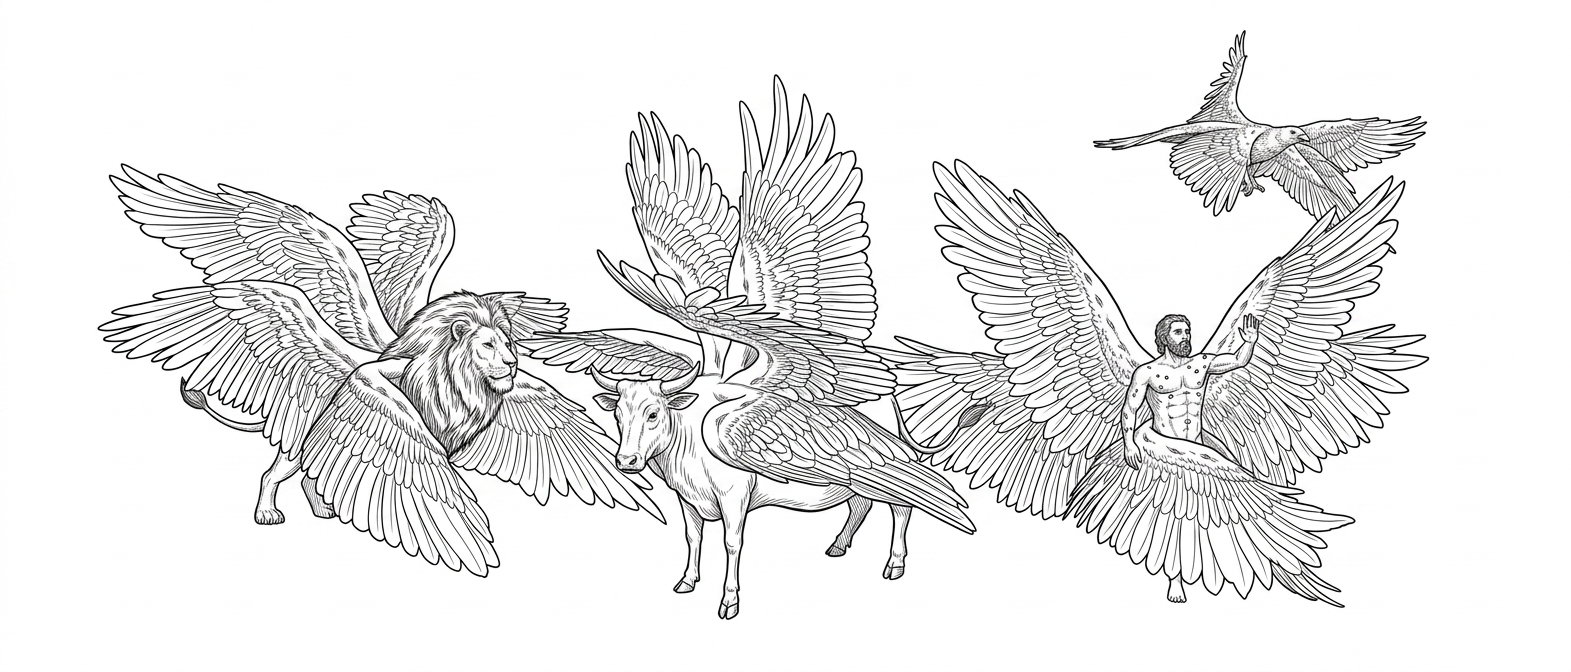
\includegraphics[
    width=1\textwidth,
    trim=100 50 100 30,
    clip]{images/four_living_creatures.jpg}
\end{figure}

The four living creatures\index{four living creatures} are beings of extraordinary power, unlike anything found among the creatures of the earth. Their bodies are covered with eyes, before and behind, within and without. They watch over all that God has made, evoking the divine knowledge that sees all things and nothing escapes His sight.\footnote{MacArthur, J. (2007); Osborne, G. R. (2002).}

Revelation 4:7 also closely parallels Ezekiel 1:10, as shown in Table \ref{table:four_creatures}:

{
\renewcommand{\arraystretch}{1}
\small
\begin{longtable}{L{4cm}L{4.5cm}}
\caption{The four living creatures in Revelation and Ezekiel}
\label{table:four_creatures} \\
\hline
\textbf{Revelation 4:7} & \textbf{Ezekiel 1:10} \\
\hline
Like a lion & The face of a lion \\
Like an ox & The face of an ox \\
Like a human being & The face of a human being \\
Like a flying eagle & The face of an eagle \\
\hline
\end{longtable}
}

\section{Praise to the Lord Who Created All Things}

% Insert the licensed NIV text of Revelation 4:10--11 in the ScriptureBox below.

\begin{ScriptureBox}

\item[4:10] the twenty-four elders fall down before him who sits on the throne and worship him who lives for ever and ever. They lay their crowns before the throne and say:

\item[4:11] \hspace*{1.5em}``You are worthy, our Lord and God,\\
\hspace*{1.5em}to receive glory and honor and power,\\
\hspace*{1.5em}for you created all things,\\
\hspace*{1.5em}and by your will they were created\\
\hspace*{1.5em}and have their being.''

\end{ScriptureBox}

The Old Testament, especially the Psalms, is filled with songs of praise to God as Creator\index{Creator}. When we read Revelation, we gain a richer understanding by setting its words alongside the related passages of Scripture. The theme of creation in Revelation 4:11 calls to mind Genesis 1, Psalm 33, Psalm 95, and Psalm 96.\footnote{Bauckham, R. (1993).}

Genesis 1 declares that in the beginning God created the heavens and the earth, and that He made humankind.

Psalm 33 proclaims the power of God's word: He speaks, and it comes to be; He commands, and it stands firm.

Psalm 95:3--7 praises the LORD as the great King above all gods. The depths of the sea, the heights of the mountains, and the whole earth belong to Him, for He made them all. Therefore, His people are called to bow down and worship Him.

Psalm 96:4--5 declares the LORD to be exalted above the gods of the nations. He made the heavens and is worthy of the worship of all peoples.

God is not merely the Creator\index{Creator} of all things; He is also the King over all creation. When the twenty-four elders\index{twenty-four elders} lay their crowns before the throne, they acknowledge that every honor and every authority possessed by created beings originates with God and must ultimately be returned to Him.

\section{No One Was Worthy to Open the Scroll}\index{scroll}

% Insert the licensed NIV text of Revelation 5:1--4 in the ScriptureBox below.

\begin{ScriptureBox}

\item[5:1] Then I saw in the right hand of him who sat on the throne a scroll with writing on both sides and sealed with seven seals.

\item[5:2] And I saw a mighty angel proclaiming in a loud voice, ``Who is worthy to break the seals and open the scroll?''

\item[5:3] But no one in heaven or on earth or under the earth could open the scroll or even look inside it.

\item[5:4] I wept and wept because no one was found who was worthy to open the scroll or look inside.

\end{ScriptureBox}

\begin{figure}[htbp]
    \centering
    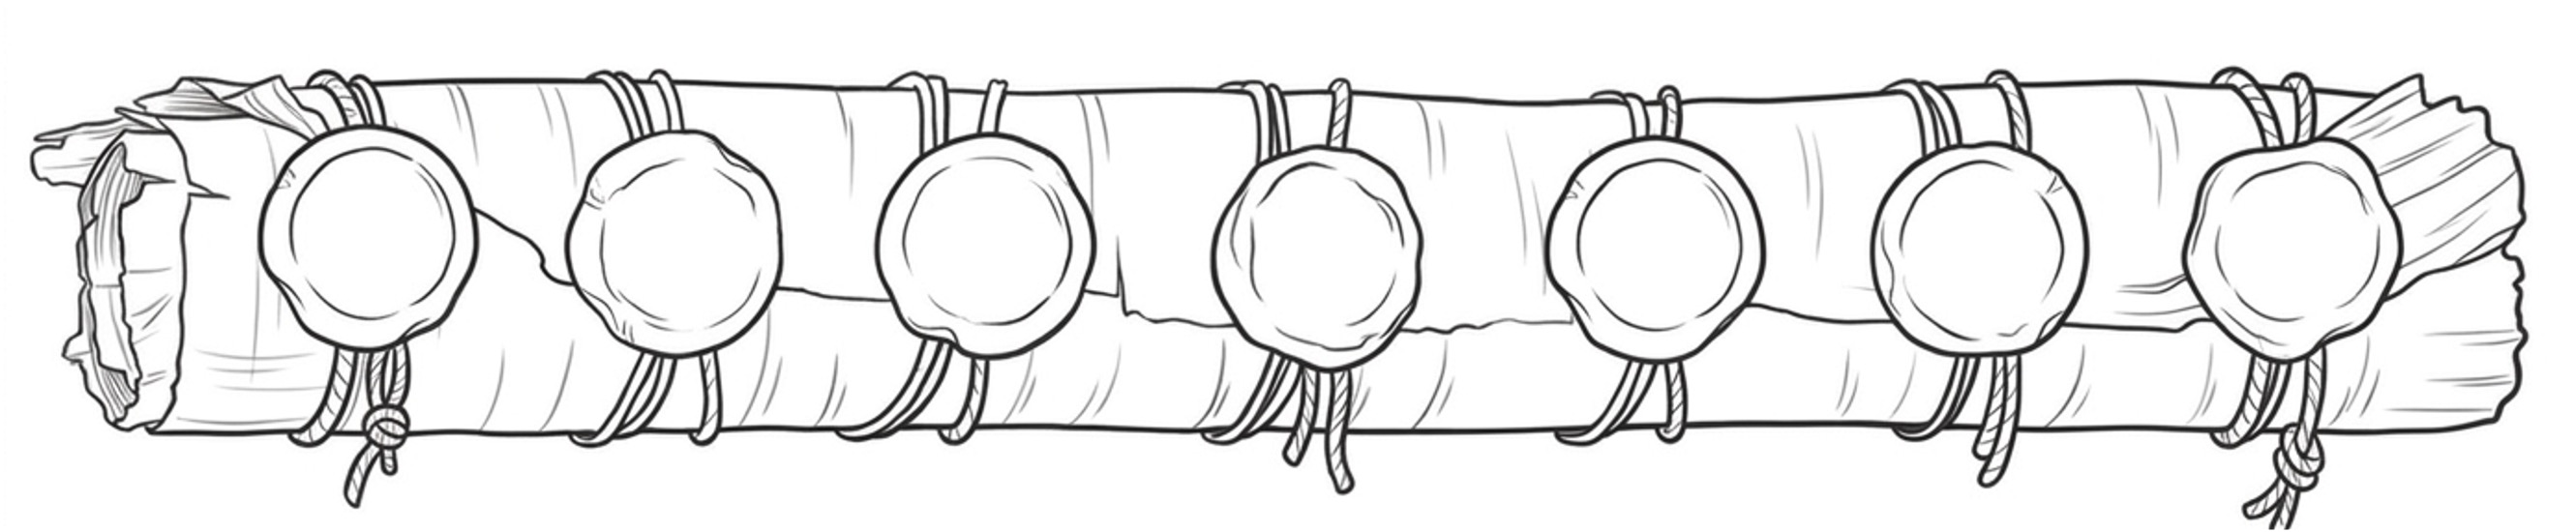
\includegraphics[
    width=1\textwidth,
    trim=0 0 0 0,
    clip]{images/scroll_light.jpg}
\end{figure}

History rests in God's hands, and the scroll\index{scroll} in His right hand holds the unfolding of His sovereign purpose. Yet who is worthy to open it, breaking its seals and bringing God's purposes to their appointed fulfillment? Not one being in all creation is found worthy. At this discovery, John weeps bitterly.

His sorrow is not merely the frustration of being unable to see what the scroll contains. The deeper anguish is that if no one is worthy to open it, no created being can bring God's plan of redemption\index{redemption} and judgment\index{judgment} into its appointed course.\footnote{This scene recalls the scroll in Ezekiel 2:9--10, which was also written on both sides. There is, however, an important difference: Ezekiel's scroll was already opened, whereas the scroll in Revelation remains sealed. Ezekiel writes, ``I looked, and I saw a hand stretched out to me. In it was a scroll, which he unrolled before me. On both sides of it were written words of lament and mourning and woe'' (Ezekiel 2:9--10, NIV).}

Why does John see an ancient scroll? If the reader lived in the modern world—or even in a distant future—would the revelation not take another form? Of course, John is not attempting to predict the technology through which future generations might publish information. He is using a means of revelation familiar to the world in which he lived.

In the ancient world, documents were commonly written on papyrus or other materials and rolled into scrolls. What John sees, therefore, is neither a modern bound book nor a digital document. The vision speaks through an image his first readers could recognize, while directing their eyes toward a purpose far greater than the scroll itself.

\section{The Slain Lamb Is the True Victorious King}\index{Lamb, the!slain}

% Insert the licensed NIV text of Revelation 5:5--7 in the ScriptureBox below.

\begin{ScriptureBox}

\item[5:5] Then one of the elders said to me, ``Do not weep! See, the Lion of the tribe of Judah, the Root of David, has triumphed. He is able to open the scroll and its seven seals.''

\item[5:6] Then I saw a Lamb, looking as if it had been slain, standing at the center of the throne, encircled by the four living creatures and the elders. The Lamb had seven horns and seven eyes, which are the seven spirits of God sent out into all the earth.

\item[5:7] He went and took the scroll from the right hand of him who sat on the throne.

\end{ScriptureBox}

Here we encounter once more the image of Jesus introduced in Chapter 1: He is the Lord who suffered and was slain, yet He is also the Lord who rose from the dead, clothed in glory and invested with authority.

The Lamb\index{Lamb, the} calls to mind His death, sacrifice, and redeeming work. The Lion of the tribe of Judah\index{Lion of the tribe of Judah} evokes His kingship, authority, and victory. Yet the Lion appears as a Lamb who has been slain. This is the wonder at the heart of Revelation: Christ accomplished redemption through His death and resurrection, and through that very victory He revealed the authority of the true King.

John then sees the Lamb with ``seven horns and seven eyes.'' The seven eyes are identified with the seven spirits\index{seven spirits} of God sent out into all the earth. In the Old Testament, a horn often symbolizes strength, power, and royal authority. The image therefore points to Christ's sovereign power and to the work of God's Spirit throughout the world.

The victorious King does not conquer\index{overcomers} as earthly rulers do. His triumph is revealed in the marks of sacrifice. The One who was slain is the One who alone is worthy to take the scroll\index{scroll} from the hand of the One seated on the throne.

\section{The Lamb Redeems People with His Own Blood}\index{redemption}\index{Lamb, the}

\begin{ScriptureBox}

\item[5:8] And when he had taken it, the four living creatures and the twenty-four elders fell down before the Lamb. Each one had a harp and they were holding golden bowls full of incense, which are the prayers of God's people.

\item[5:9] And they sang a new song, saying:\\
\hspace*{1.5em}``You are worthy to take the scroll\\
\hspace*{1.5em}and to open its seals,\\
\hspace*{1.5em}because you were slain,\\
\hspace*{1.5em}and with your blood you purchased for God\\
\hspace*{1.5em}persons from every tribe and language and people and nation.

\item[5:10] \hspace*{1.5em}You have made them to be a kingdom and priests to serve our God,\\
\hspace*{1.5em}and they will reign on the earth.''

\end{ScriptureBox}

Through His own blood, the Lamb has redeemed people from every nation and brought them to God.

This is the song of sinners who have been overtaken by grace\index{grace}. Their voices bear witness to the astonishing mercy of God, to lives transformed by His saving work, and ultimately to the glory into which He brings His redeemed people.

Christ does more than forgive our sins. He grants us a new identity, making us a kingdom and priests who belong to God. Those who were once far from Him are brought near. Those who once had no claim to stand among the worshipers of heaven are now welcomed to join their song of praise to the Lamb.

Grace has changed their standing before God, and it has changed the direction of their lives. They belong to the One who purchased them with His blood. Their redemption is not the end of their story, but the beginning of a life devoted to the worship and service of their Redeemer.

\section{From John's Weeping to the Worship of the Whole Universe}\index{worship}

\begin{ScriptureBox}

\item[5:11] Then I looked and heard the voice of many angels, numbering thousands upon thousands, and ten thousand times ten thousand. They encircled the throne and the living creatures and the elders.

\item[5:12] In a loud voice they were saying:\\
\hspace*{1.5em}``Worthy is the Lamb, who was slain,\\
\hspace*{1.5em}to receive power and wealth and wisdom and strength\\
\hspace*{1.5em}and honor and glory and praise!''

\item[5:13] Then I heard every creature in heaven and on earth and under the earth and on the sea, and all that is in them, saying:\\
\hspace*{1.5em}``To him who sits on the throne and to the Lamb\\
\hspace*{1.5em}be praise and honor and glory and power,\\
\hspace*{1.5em}for ever and ever!''

\item[5:14] The four living creatures said, ``Amen,'' and the elders fell down and worshiped.

\end{ScriptureBox}

%\begin{figure}[htbp]
%    \centering
%    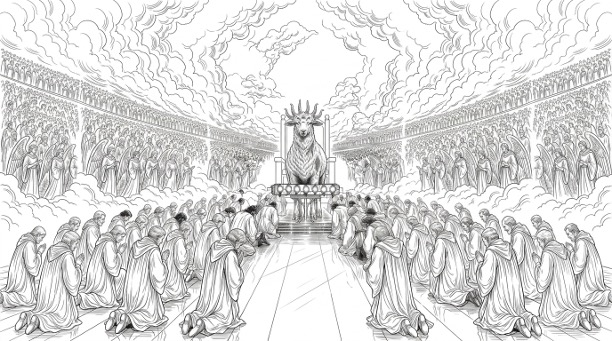
\includegraphics[
%    width=1\textwidth,
%    trim=0 0 0 0,
%    clip]{images/lamb_get_scroll2.jpg}
%\end{figure}

What a magnificent chorus of praise! The circle of worship expands from countless angels around the throne to every creature in heaven, on earth, beneath the earth, and in the sea. All creation joins in ascribing praise, honor, glory, and power to the One seated on the throne and to the Lamb, forever and ever.

Chapter 4 presents the worship due to God because He created all things. Chapter 5 reveals the worship due to the Lamb because He accomplished redemption. Creation and redemption converge in one great act of adoration: the Lamb who was slain\index{Lamb, the!slain}, and who lives forever, receives eternal worship together with the One seated on the throne.

Table \ref{table:rev4_5_praise} summarizes the relationship between these two chapters for their reason of praise, worshipers, and central message.

{
\renewcommand{\arraystretch}{1}
\small
\begin{longtable}{L{4.5cm}L{4.5cm}}
\caption{Praise for creation and praise for redemption in Revelation 4--5}
\label{table:rev4_5_praise} \\
\hline
\textbf{Chapter 4: Praise for Creation} & \textbf{Chapter 5: Praise for Redemption} \\
\hline
The Lord seated on the throne &
The Lord seated on the throne and the Lamb \\

God created all things &
The Lamb was slain and redeemed people with His blood \\

Glory, honor, power, and the creation of all things &
Power, wealth, wisdom, strength, honor, glory, and praise \\

The four living creatures and the twenty-four elders &
The four living creatures, the twenty-four elders, countless angels, and all created beings \\

All things were created according to God's will &
People from every nation are redeemed by the Lamb's blood and brought to God \\
\hline
\end{longtable}
}

Creation and redemption meet in this heavenly vision. The Lamb who was slain\index{Lamb, the!slain}, and who now lives, receives eternal worship together with God upon the throne.

May we praise Him each day for the power by which He created all things, letting our words of praise surge like the boundless sea. May we also give thanks each day for the grace by which He redeemed us, letting our gratitude flow like a mighty river, never running dry.

For we were not merely brought into existence by the Creator\index{Creator}; through the blood of the Lamb\index{Lamb, the!blood of}, we have been brought near to Him. The One who reigns over all creation has made a way for sinners to stand before His throne. Here lies the wonder of grace: those who once had no reason to boast now have every reason to worship.

\section*{Discussion Questions}

\begin{enumerate}

\item In the days when Israel faced national disaster and God's people endured suffering, Ezekiel and Isaiah were also given visions of God's glorious throne. How do these visions help us understand that God remains sovereign over history? What do they teach us when we face hardship and uncertainty in our own lives?

\item The four living creatures proclaim without ceasing, ``Holy, holy, holy is the Lord God Almighty, who was, and is, and is to come.'' What do God's holiness, eternity, and omnipotence mean for our worship today? How should these truths shape the way we approach Him?

\item Genesis 1 and Psalms 33, 95, and 96 praise God's creation from different perspectives. How should recognizing God as the Creator of all things change the way we view our lives, our work, and the created world around us?

\end{enumerate}

\chapter{The Lamb Opens the Scroll (6:1--7:17)}

In heaven, the Lamb opens the seals; on earth, judgment unfolds.

The first four seals reveal judgment upon the earth through conquest, war, famine, and death. The fifth turns our gaze toward the souls of those who were martyred because of the word of God and their faithful testimony. When the sixth seal is opened, the heavens and the earth are shaken, and the stars fall from the sky. The great day of the Lamb's wrath has come, and the people of the earth cry out in terror: ``Who can withstand it?''

Revelation 7 answers this question. Only those who belong to God, cleansed by the blood of the Lamb, can stand before the throne and before the Lamb. Thus, the seven seals reveal not only the fearsome reality of divine judgment but also God's preserving care for His people, the salvation accomplished by the Lamb, and the eternal hope that awaits the redeemed.

\section{The First Four Seals: The Four Horsemen}

% Insert the licensed NIV text of Revelation 6:1--8 in the ScriptureBox below.

\begin{ScriptureBox}

\item[6:1] I watched as the Lamb opened the first of the seven seals. Then I heard one of the four living creatures say in a voice like thunder, ``Come!''

\item[6:2] I looked, and there before me was a white horse! Its rider held a bow, and he was given a crown, and he rode out as a conqueror bent on conquest.

\item[6:3] When the Lamb opened the second seal, I heard the second living creature say, ``Come!''

\item[6:4] Then another horse came out, a fiery red one. Its rider was given power to take peace from the earth and to make people kill each other. To him was given a large sword.

\item[6:5] When the Lamb opened the third seal, I heard the third living creature say, ``Come!'' I looked, and there before me was a black horse! Its rider was holding a pair of scales in his hand.

\item[6:6] Then I heard what sounded like a voice among the four living creatures, saying, ``Two pounds of wheat for a day's wages, and six pounds of barley for a day's wages, and do not damage the oil and the wine!''

\item[6:7] When the Lamb opened the fourth seal, I heard the voice of the fourth living creature say, ``Come!''

\item[6:8] I looked, and there before me was a pale horse! Its rider was named Death, and Hades was following close behind him. They were given power over a fourth of the earth to kill by sword, famine and plague, and by the wild beasts of the earth.

\end{ScriptureBox}

\begin{figure}[htbp]
    \centering
    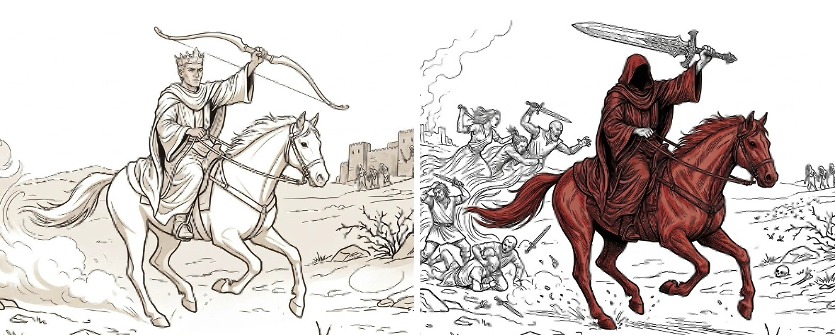
\includegraphics[
    width=1\textwidth,
    trim=0 0 0 00,
    clip]{images/horses_white_red.png}
    \caption{The 1st and 2nd Seals}
    \label{fig:horses_white_red.png}
\end{figure}

The four horses and their riders bring a succession of conquest, war, famine, and death upon the earth.

The white horse rides forth to conquer and conquer again. The red horse brings bloodshed. The black horse brings famine and poverty. The pale horse brings death.

I use the following mnemonic to help remember the distinctive role of each horse:

\begin{center}
\begin{tabular}{l}
\hline
White to conquer \\
Red to kill \\
Black to famine \\
Pale to die \\
\hline
\end{tabular}
\end{center}

\begin{figure}[htbp]
    \centering
    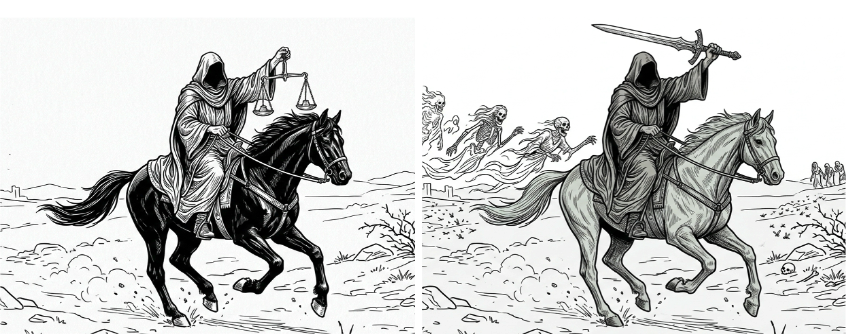
\includegraphics[
    width=1\textwidth,
    trim=0 0 0 0,
    clip]{images/horses_black_gray.png}
    \caption{The 3rd and 4th Seals}
    \label{fig:horses_black_gray.png}
\end{figure}

The words ``a quart of wheat for a day's wages'' portray the famine that often follows war, when food becomes scarce and prices soar. During wartime, armies frequently obtain provisions by plundering the countryside, sometimes seizing food by force and leaving villages stripped of their supplies. Famine is one of the devastating consequences that war leaves in its wake.

Wheat and barley were important staples throughout the Roman Empire. Wheat was generally considered the better grain and served as a principal food, while barley was less expensive and more commonly consumed by poorer people. A quart of wheat represented approximately one person's daily portion, while three quarts of barley provided a roughly comparable daily supply of grain.

A denarius, or silver coin, commonly represented a laborer's wages for one day's work. A person might therefore labor throughout the day only to earn enough to purchase the wheat needed for that day's food. Even if he bought barley instead, his wages would barely cover his basic portion. Supporting a family, paying for shelter, and meeting other daily expenses would be harder still.

This is the terrible condition the vision portrays: food remains available, but its price has risen beyond what ordinary people can reasonably afford. Olive oil and wine, even more precious in a time of scarcity, are not to be wasted. When even the daily necessities of life become difficult to obtain, every remaining resource matters.

The red, black, and pale horses are relatively straightforward to understand from the text. But who is the rider on the white horse? Biblical interpreters have generally proposed three major interpretations.

\begin{enumerate}

\item \textbf{The white horse represents a false Christ or the forces of the Antichrist.}

This is the view widely held by many futurist interpreters; see the appendix, ``Various Views of the End Times.''\footnote{MacArthur, J. (2007).}

The rider carries a bow, yet no arrows are mentioned. Some interpreters take this detail to suggest conquest through deception, political maneuvering, or the appearance of peaceful success. They also connect the rider with the beast and the forces of the Antichrist described later in Revelation. Thus, the first seal marks the beginning of the Antichrist's activity in the last days.

Matthew 24:4--5 warns that false messiahs will deceive many before Jesus speaks of wars and famines. The resemblance between the sequence in Matthew and the four horsemen lends support to this interpretation.

\item \textbf{The white horse represents military conquest.}

Other interpreters argue that the rider need not be the Antichrist. Since the text explicitly says that he went out ``as a conqueror bent on conquest,'' they understand him to symbolize military expansion and imperial aggression more generally.

Conquest often leads to war, famine, and death. Thus, the four horsemen form a connected sequence: the ambitions of conquest give rise to bloodshed, scarcity, and widespread mortality.

\item \textbf{The white horse represents Christ or the victory of the gospel.}

This is a less widely held interpretation. Those who support it point out that white often symbolizes holiness and victory in Revelation. In Revelation 19:11, Christ Himself rides a white horse, and the rider's continuing conquest in Revelation 6:2 may be understood as the advancing triumph of the gospel.

However, many modern interpreters do not accept this view. They argue that the four horsemen should be understood together as a unified group, and that significant differences remain between the rider in Revelation 6 and Christ on the white horse in Revelation 19.

\end{enumerate}

\section{The Fifth Seal: The Cry of the Martyrs}

% Insert the licensed NIV text of Revelation 6:9--11 in the ScriptureBox below.

\begin{ScriptureBox}

\item[6:9] When he opened the fifth seal, I saw under the altar the souls of those who had been slain because of the word of God and the testimony they had maintained.

\item[6:10] They called out in a loud voice, ``How long, Sovereign Lord, holy and true, until you judge the inhabitants of the earth and avenge our blood?''

\item[6:11] Then each of them was given a white robe, and they were told to wait a little longer, until the full number of their fellow servants, their brothers and sisters, were killed just as they had been.

\end{ScriptureBox}

In the eyes of many Romans, the followers of Jesus were misguided and superstitious. To give one's life in allegiance to a Messiah who had been crucified seemed absurd, even ridiculous. Some surviving historical records offer a sobering glimpse of the hostility Christians faced.\footnote{Koester, C. R. (2014).}\footnote{Tacitus, \textit{Ann.} 15.44; Pliny the Younger, \textit{Ep.} 10.96.8.}\footnote{\textit{Mart. Carp.} 9.}

The martyrs were killed because of the word of God and their testimony. They had remained faithful in proclaiming God's truth and bearing witness to Him, yet their faithfulness brought them suffering and death. What a profound injustice!

For Christians who faced persecution and martyrdom in the first century, this vision would have offered extraordinary comfort. Though rejected and killed on earth, the martyrs beneath the altar were not forgotten. They were received into God's presence, and their cries reached the ears of the Holy and True One.

Their testimony teaches us three important lessons:

\begin{enumerate}
\item Remain faithful in bearing witness to God, even when faithfulness demands the ultimate sacrifice (6:9).
\item Bring our grievances before the Holy and Righteous Lord rather than taking vengeance into our own hands (6:10).
\item While the fullness of justice is still awaited, receive God's assurance and continue to endure in faith (6:11).
\end{enumerate}

You may ask, however: Did the Lord Jesus not teach us to love our enemies and pray for those who persecute us? How, then, should we understand the martyrs' cry for justice?

The key is to recognize the injustice suffered by the victims. These believers were persecuted and killed because they remained loyal to Christ. Their appeal to God was not a demand for permission to take personal revenge. Rather, they entrusted judgment to the righteous Judge.

The passage assures us that the God who is holy and true does not forget those who faithfully follow Him and bear witness to His name. If the martyrs confess that God is ``holy and true,'' can He remain forever indifferent when the wicked shed innocent blood?

God's judgment comes at the time He has appointed. Even the completion of the number of martyrs belongs to His sovereign purpose. The final judgment will not occur according to human impatience, but according to God's perfect wisdom.

The fact that God does not immediately execute final judgment does not mean that He overlooks evil or has forgotten His promises. Rather, in His mercy and patience, He continues to give people an opportunity to repent. As 2 Peter 3:9--10 explains, the apparent delay of the Lord's promise reflects His patience and His desire that people should come to repentance. Yet the day of the Lord will come like a thief, and the present order will not endure forever.

The same patience that grants sinners time to turn back to God also calls His people to persevere. We may grieve over injustice, and we may cry out for the Lord to act. But we do so in the confidence that history remains in His hands and that His justice will not fail.

\section{The Sixth Seal: The Stars Fall from the Sky}

\begin{ScriptureBox}

\item[6:12] I watched as he opened the sixth seal. There was a great earthquake. The sun turned black like sackcloth made of goat hair, the whole moon turned blood red,

\item[6:13] and the stars in the sky fell to earth, as figs drop from a fig tree when shaken by a strong wind.

\item[6:14] The heavens receded like a scroll being rolled up, and every mountain and island was removed from its place.

\item[6:15] Then the kings of the earth, the princes, the generals, the rich, the mighty, and everyone else, both slave and free, hid in caves and among the rocks of the mountains.

\item[6:16] They called to the mountains and the rocks, ``Fall on us and hide us from the face of him who sits on the throne and from the wrath of the Lamb!

\item[6:17] For the great day of their wrath has come, and who can withstand it?''
% NIV footnotes for 6:16--17 (omitted; add as \footnote if wanted):
%   6:16 ``hide us'' --- See Hosea 10:8.
%   6:17 ``their'' --- Some manuscripts his
\end{ScriptureBox}

\begin{figure}[htbp]
    \centering
    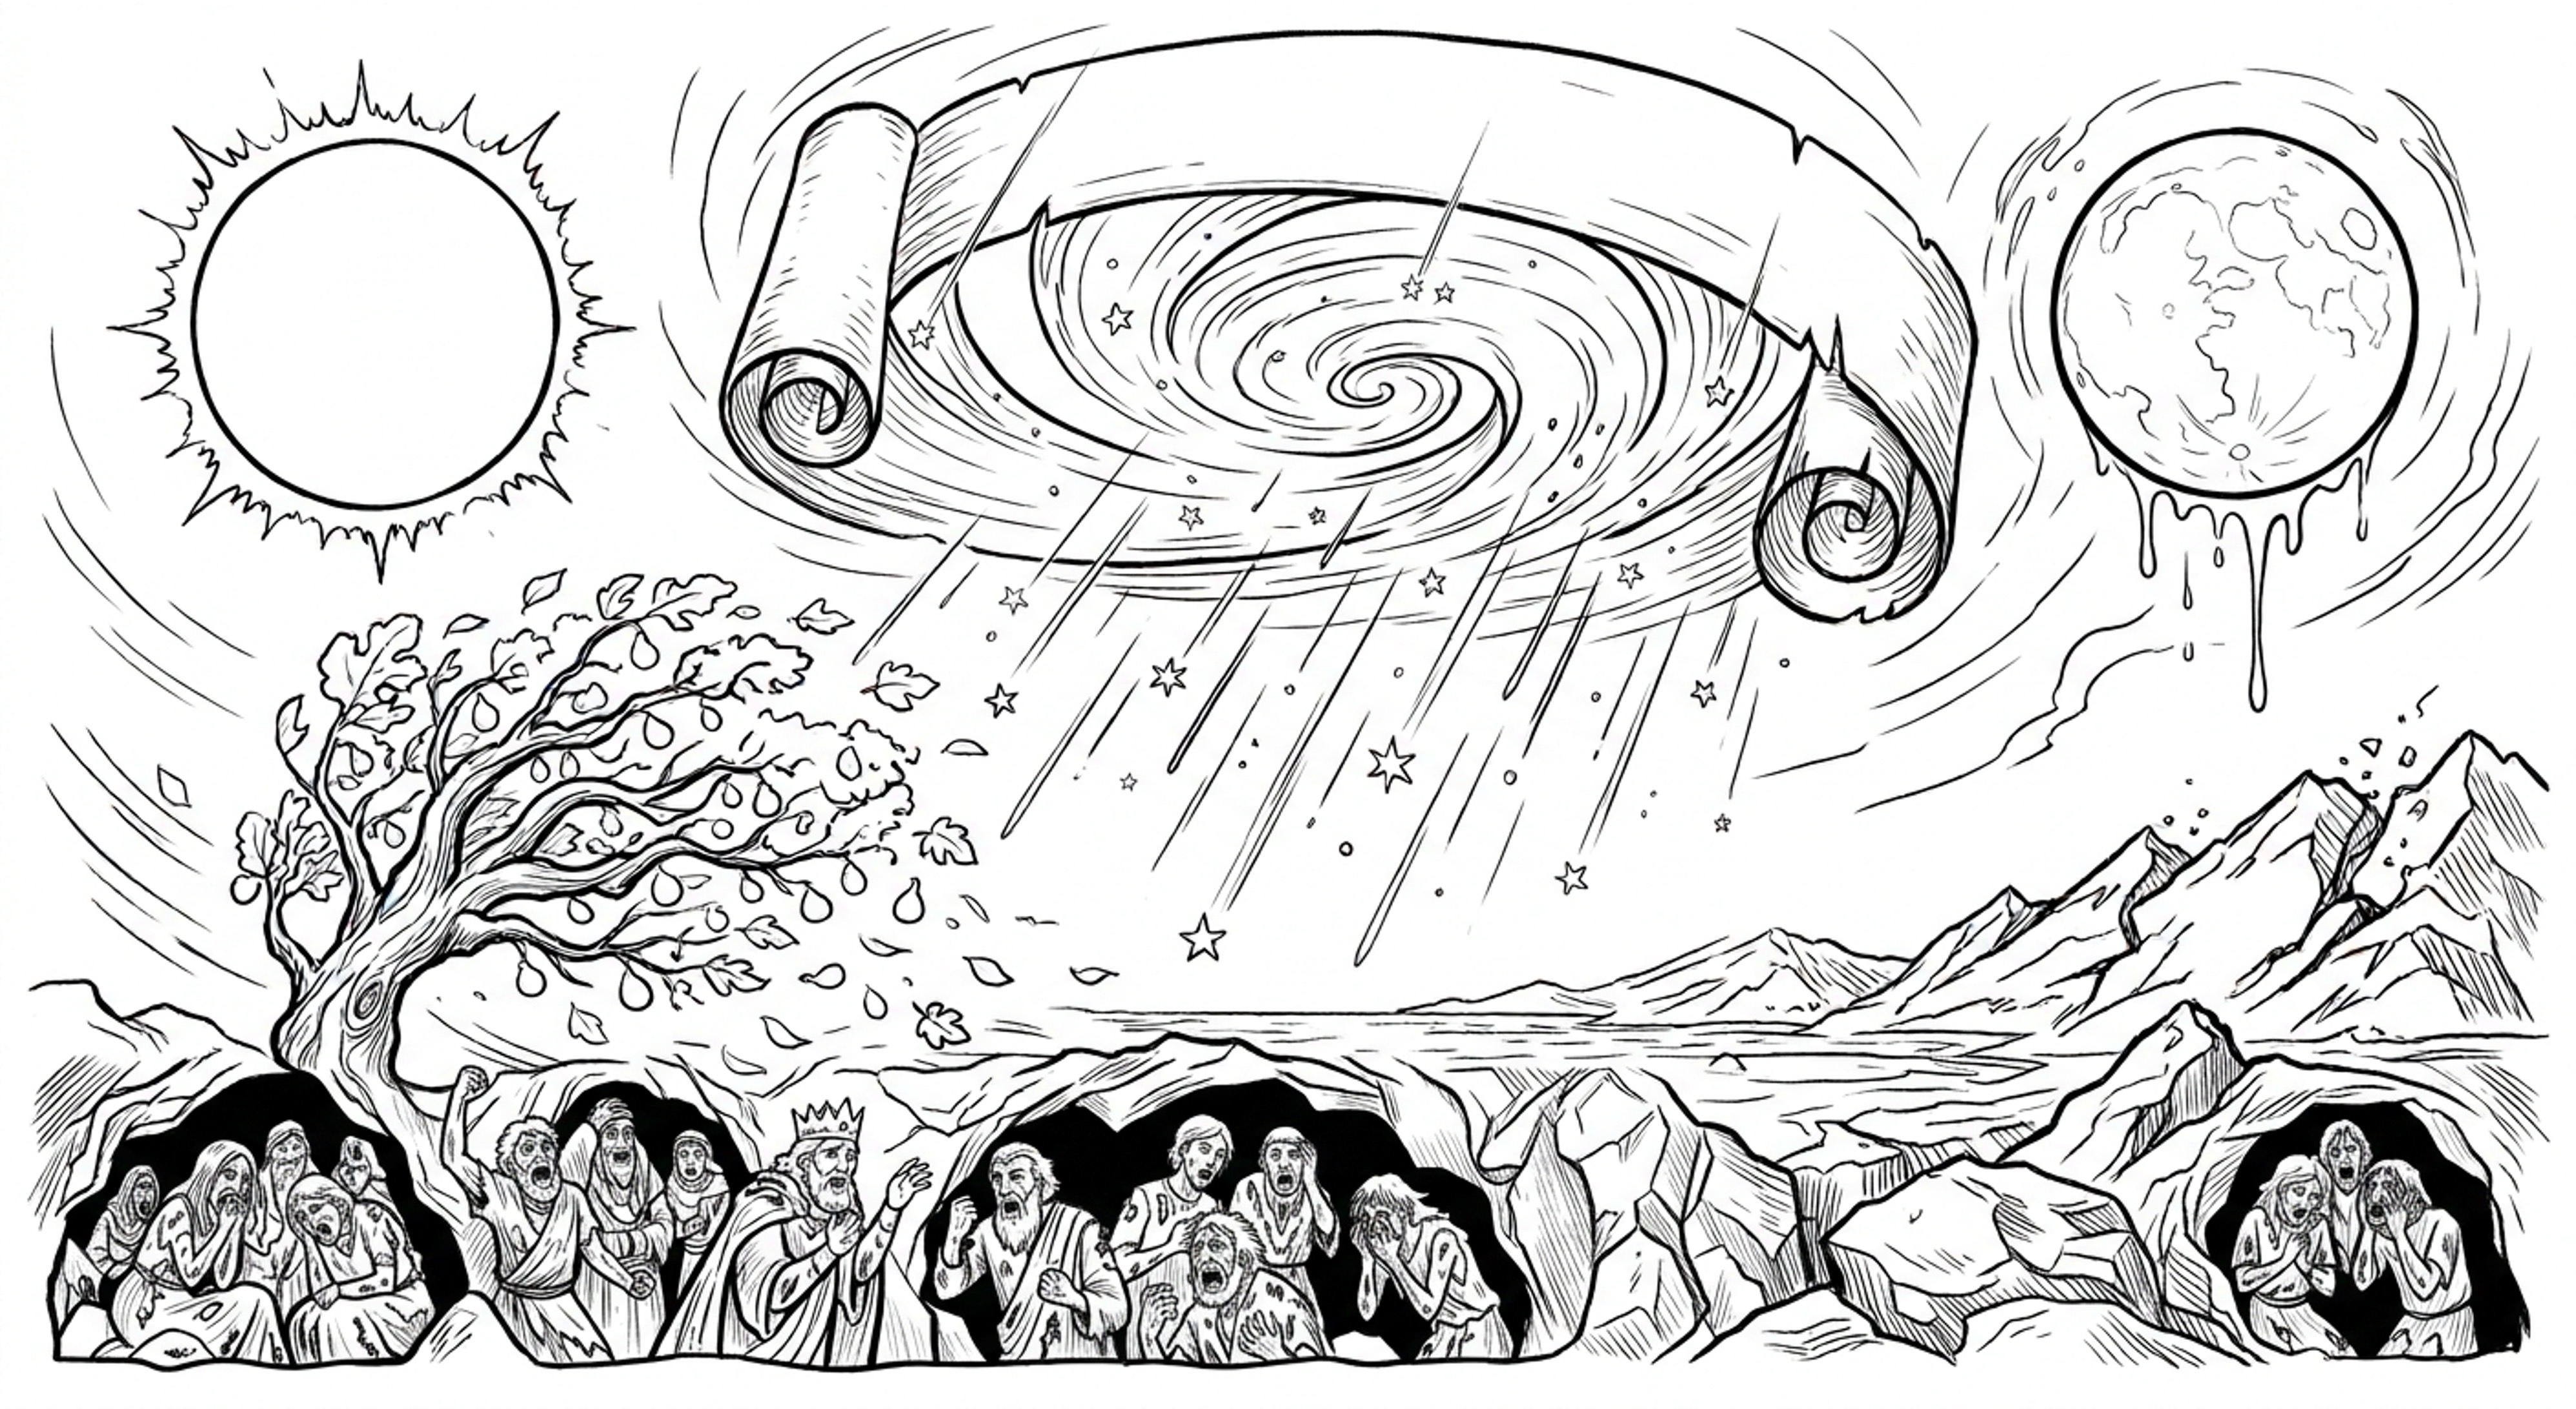
\includegraphics[
    width=1\textwidth,
    trim=0 0 0 0,
    clip]{images/seal_6th.jpg}
    \caption{The 6th Seal: The Stars Fall from the Sky}
    \label{fig:seal_6th}
\end{figure}

The heavens and the earth are shaken. The familiar order of creation seems to come apart, and the people of the earth find nowhere to hide. In terror, they ask who can stand before the righteous wrath of the Lamb.

Yet Revelation 7 will show us the answer. Those who have been redeemed by the blood of the Lamb will stand before the throne and before Him, as shown in Table \ref{tab:who-can-stand}.

{
\small
\renewcommand{\arraystretch}{1}
\begin{longtable}{p{0.43\textwidth} p{0.43\textwidth}}
\caption{Who can stand?}
\label{tab:who-can-stand} \\
\hline
Revelation 6:15--17 & Revelation 7:9--14 \\
\hline
\endfirsthead

\multicolumn{2}{l}{\small\itshape Table~\thetable\ (continued)} \\
\hline
Revelation 6:15--17 & Revelation 7:9--14 \\
\hline
\endhead

\hline
\endfoot

\hline
\endlastfoot

People hide from the face of God and the Lamb & A great multitude stands before God and the Lamb \\
They tremble at the coming day of wrath & They wear white robes and worship God \\
They ask, ``Who can stand?'' & The blood of the Lamb enables the redeemed to stand \\
\end{longtable}
}

This contrast captures the central message of these chapters.

When we face the righteous wrath of the Lamb, will we be able to stand before Him? The answer does not lie in our own good works or strength. It rests in the Lamb, who shed His blood for us, redeemed us, and cleansed us from sin.

Even today, Christ extends His gracious invitation to us. My hope is that every reader of this book will receive the Lamb's invitation rather than wait until that dreadful day and seek to hide from His presence.

If you have not yet turned to Christ, now is the time to repent and place your trust in His saving work. By the grace of the Lamb, you too may join the multitude clothed in white, standing before Him and giving glory and praise to God.

\subsection*{The First Six Seals and Matthew 24}

The Olivet Discourse, in which Jesus speaks about the events to come in Matthew 24, bears striking parallels to the first six seals in Revelation.
Table \ref{tab:seals-matthew24} shows the parallels.
{
\small
\renewcommand{\arraystretch}{1}
\begin{longtable}{>{\raggedright\arraybackslash}p{0.27\textwidth}
                  >{\raggedright\arraybackslash}p{0.33\textwidth}
                  >{\raggedright\arraybackslash}p{0.25\textwidth}}
\caption{The six seals of Revelation 6 and the signs in Matthew 24}
\label{tab:seals-matthew24} \\
\hline
Seal & Matthew 24 & Correspondence \\
\hline
\endfirsthead

\multicolumn{3}{l}{\small\itshape Table~\thetable\ (continued)} \\
\hline
Seal & Matthew 24 & Correspondence \\
\hline
\endhead

\endfoot

\endlastfoot

\ding{172} The white horse: its rider goes out conquering and to conquer &
\textsuperscript{4--5} Many come in Christ's name and deceive many &
False messiahs and deceptive claims of peace. \\
\hline
\ding{173} The red horse: peace is taken from the earth, and people kill one another &
\textsuperscript{6--7} Wars and rumors of wars; nation rises against nation and kingdom against kingdom &
War, violence, and social upheaval. \\
\hline
\ding{174} The black horse: scales and expensive grain &
\textsuperscript{7} Famines in various places &
Food shortages and economic hardship. \\
\hline
\ding{175} The pale horse: death and the realm of the dead &
\textsuperscript{7--9} Famines, earthquakes, and believers handed over to suffering &
Death, disasters, and affliction. \\
\hline
\ding{176} The martyrs cry out for justice &
\textsuperscript{9--13} Believers suffer persecution, are killed and hated, and are called to endure to the end &
Persecution, martyrdom, and perseverance. \\
\hline
\ding{177} Earthquake, darkened sun and moon, and falling stars &
\textsuperscript{29--30} The sun and moon are darkened, the stars fall, and the Son of Man appears in heaven &
Cosmic upheaval and the coming of the Son of Man. \\
\hline
\end{longtable}
}

Matthew 24 and the vision of the seven seals each have their own emphasis. Matthew stresses the need for Jesus' disciples to remain alert, endure to the end, and await the coming of the Son of Man. Revelation develops these themes through the vision of the Lamb opening the scroll, showing that history and judgment remain under the sovereign authority of Christ.

The parallels are significant, but they do not require every detail to correspond to an identical event or a precise timetable. Both passages call believers to discernment and endurance while keeping their eyes fixed on the Lord who will bring history to its appointed end.

\section{The Seventh Seal}

% Insert the licensed NIV text of Revelation 8:1 in the ScriptureBox below.

\begin{ScriptureBox}
\item[8:1] \textit{When he opened the seventh seal, there was silence in heaven for about half an hour.}
\end{ScriptureBox}

The seventh seal appears in Revelation 8:1. We introduce it here alongside the first six seals because it completes the sequence, even though the biblical account continues into the next chapter.

Unlike the first six seals, the seventh does not immediately portray a distinct calamity. Instead, it introduces the vision of the seven trumpets (8:2). Through these trumpets, God's judgments continue to unfold, carrying the vision into a new stage.

When the Lamb opens the seventh seal, silence falls over heaven for about half an hour. The silence is like a rest in a great symphony. The heavenly hosts fall still, and the entire court of heaven seems to hold its breath, awaiting the solemn and terrible movement that is about to begin.

This silence does not signal the end of judgment. It is a moment of awe-filled stillness before the next great movement of divine judgment breaks forth.

\subsection*{The Sequence of the Seven Seals, Seven Trumpets, and Seven Bowls}

The seventh seal introduces the seven trumpets. When the seventh trumpet sounds, a heavenly proclamation announces the kingdom of God and of Christ, and speaks of God's wrath, the judgment of the dead, and the rewarding of the prophets and saints (11:18).

Yet the seven bowls do not immediately follow the seventh trumpet. Between them stand the visions in Chapters 12--14: the woman and the dragon, the two beasts, the Lamb with the 144,000, and the messages of the three angels. In Chapter 15, John sees seven angels holding the seven last plagues, and is told that with them God's wrath is completed (15:1). Chapter 16 then describes the pouring out of the seven bowls.

To give readers an overview, Figure \ref{fig:seals_trumpets_bowls} illustrates the sequence of the seals, trumpets, and bowls. The following discussion addresses a related interpretive question.

\begin{figure}[htbp]
    \centering
    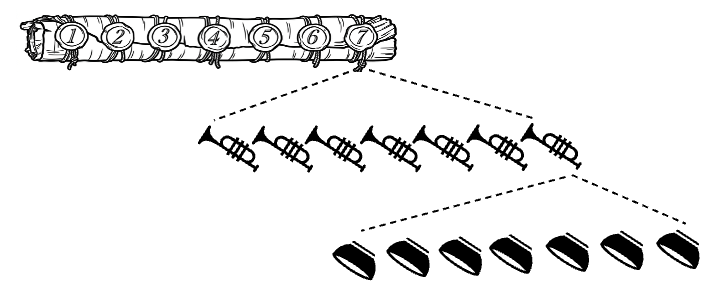
\includegraphics[
    width=1\textwidth,
    trim=0 0 0 0,
    clip]{images/seals_trumpets_bowls.png}
    \caption{The Sequence of the Seven Seals, Seven Trumpets, and Seven Bowls}
    \label{fig:seals_trumpets_bowls}
\end{figure}

Because many of the judgments among the seals, trumpets, and bowls appear to resemble one another, an important question naturally arises.

\subsection*{Do the Seven Seals, Seven Trumpets, and Seven Bowls Occur in Sequence, or Do They Recapitulate the Same Final Judgment?}

Read at face value, the seven seals, seven trumpets, and seven bowls appear in succession. But could they instead describe the same events from different perspectives, each time intensifying the portrayal of judgment? Interpreters have proposed two broad approaches to the relationship between these three series of visions. Table \ref{tab:seals-trumpets-bowls} shows the comparison.

{
\small
\renewcommand{\arraystretch}{1}
\begin{longtable}{>{\raggedright\arraybackslash}p{0.15\textwidth}|
                  >{\raggedright\arraybackslash}p{0.35\textwidth}|
                  >{\raggedright\arraybackslash}p{0.4\textwidth}}
\caption{Two views of the seals, trumpets, and bowls}
\label{tab:seals-trumpets-bowls} \\
\hline
 & Successive Judgments & Recapitulation with Increasing Intensity \\
\hline
\endfirsthead

\multicolumn{3}{l}{\small\itshape Table~\thetable\ (continued)} \\
\hline
 & Successive Judgments & Recapitulation with Increasing Intensity \\
\hline
\endhead

\endfoot

\endlastfoot

Seals & The seventh seal introduces the seven trumpets. & The seals portray God's judgment upon the world. \\
\hline
Trumpets & The trumpets follow the seventh seal. & The trumpets revisit the theme of judgment from another perspective and intensify it. \\
\hline
Bowls & The bowls follow the trumpets and bring God's wrath to its full expression. & The bowls present another recapitulation of divine judgment. \\
\hline
Evidence & The seventh seal introduces the trumpets, and the bowls appear after the trumpet visions. & The sixth seal, seventh trumpet, and seventh bowl all employ language associated with final judgment. \\
\hline
Strength & Emphasizes the apparent chronological sequence of the visions. & Helps explain the recurring images of cosmic upheaval, divine wrath, and judgment upon the nations. \\
\hline
\end{longtable}
}

These two approaches are not necessarily mutually exclusive in every respect. Interpreters who favor recapitulation do not always deny the sequence presented in the text. Rather, they understand that sequence as part of a literary structure in which related visions may overlap or portray events from different perspectives.

For this reason, we should be cautious about assigning each judgment to a specific modern historical event solely on the basis of the order in which the visions appear.

You may ask: When will the seven seals take place? Will they occur only during a future great tribulation, or did they begin in the apostolic age and continue until Christ's return? Could they also portray patterns of suffering and judgment that recur throughout history?

Christian theologians have offered several interpretations of these questions. I discuss them in greater detail in the appendix, ``Various Views of the End Times.''

We now turn to Revelation 7, where John sees 144,000 people sealed, followed by a multitude beyond counting, drawn from every nation, tribe, people, and language, standing before the throne and the Lamb.

\section{The Seal of the Living God Preserves His Servants}


\begin{ScriptureBox}

\item[7:1] After this I saw four angels standing at the four corners of the earth, holding back the four winds of the earth to prevent any wind from blowing on the land or on the sea or on any tree.

\item[7:2] Then I saw another angel coming up from the east, having the seal of the living God. He called out in a loud voice to the four angels who had been given power to harm the land and the sea:

\item[7:3] ``Do not harm the land or the sea or the trees until we put a seal on the foreheads of the servants of our God.''

\end{ScriptureBox}

You may have noticed that between the sixth and seventh seals, the narrative suddenly pauses to introduce Revelation 7 and the sealing of God's servants by the living God. Why is this vision placed here?

The answer lies in the question with which Revelation 6:17 ends: ``For the great day of their wrath has come, and who can withstand it?'' Revelation 7 responds directly. Those who belong to God—the servants who bear His seal and the multitude clothed in white—are seen standing before the throne and the Lamb.\footnote{Beale, G. K. (1999).}

The expression ``the four winds'' draws upon Old Testament imagery for forces that affect the whole earth.\footnote{Daniel 7:2 speaks of ``the four winds of heaven'' churning up the great sea; Jeremiah 49:36 describes God bringing the four winds against Elam and scattering its people in every direction.} We therefore need not evaluate ``the four corners of the earth'' or ``the four winds'' through the lens of modern geometry or meteorology. The point is not the physical shape of the earth, but God's authority over the whole world and His sovereign control over the timing of judgment.

Why are God's servants sealed before judgment proceeds? This is a central point of the vision. The seal is not an incidental detail added to the judgment scene; it identifies those who belong to God and expresses His redemptive care for them. Let us consider who receives this seal.

\section{The Twelve Tribes of Israel}

% Insert the licensed NIV text of Revelation 7:4 and 7:8 in the ScriptureBox below.

\begin{ScriptureBox}

\item[7:4] Then I heard the number of those who were sealed: 144,000 from all the tribes of Israel.

\item[7:5] From the tribe of Judah 12,000 were sealed,\\
from the tribe of Reuben 12,000,\\
from the tribe of Gad 12,000,

\item[7:6] from the tribe of Asher 12,000,\\
from the tribe of Naphtali 12,000,\\
from the tribe of Manasseh 12,000,

\item[7:7] from the tribe of Simeon 12,000,\\
from the tribe of Levi 12,000,\\
from the tribe of Issachar 12,000,

\item[7:8] from the tribe of Zebulun 12,000,\\
from the tribe of Joseph 12,000,\\
from the tribe of Benjamin 12,000.

\end{ScriptureBox}

John records that 144,000 people are sealed. Who are they? The number may be understood literally, though it may also carry symbolic significance. Three major interpretations are commonly proposed:

{
\small
\renewcommand{\arraystretch}{1}
\begin{longtable}{>{\raggedright\arraybackslash}p{2.4cm}
                  >{\raggedright\arraybackslash}p{6.6cm}}
\hline
Interpretation & Explanation \\
\hline
\endfirsthead

\hline
Interpretation & Explanation \\
\hline
\endhead

\endfoot

\endlastfoot

Israel &
The 144,000 are people sealed from the twelve tribes of Israel in the last days. \\
\hline
The church  &
The number represents the complete people of God, consisting of Jewish and Gentile believers. \\
\hline
Israel as a symbol &
The twelve tribes symbolize God's people in the last days, emphasizing His complete preservation of those who belong to Him. \\
\hline
\end{longtable}
}

Throughout Revelation, the number twelve appears repeatedly: the twelve tribes, the twelve apostles, the twelve gates, the twelve foundations, and the twelve gates of the New Jerusalem (Revelation 21:12--14). The carefully structured number 144,000 therefore resonates with Revelation's recurring use of twelve to represent the fullness and completeness of God's people.

Some writers attempt to identify precisely which individuals belong to this number. Such speculation, however, seems to go beyond what this passage is intended to establish. The central emphasis is that God knows those who belong to Him. When judgment comes upon the earth, He does not forget His people; He recognizes them and holds them within His sovereign care.

\section{The Worship of All Nations and the Salvation of the Lamb}


\begin{ScriptureBox}

\item[7:9] After this I looked, and there before me was a great multitude that no one could count, from every nation, tribe, people and language, standing before the throne and before the Lamb. They were wearing white robes and were holding palm branches in their hands.

\item[7:10] And they cried out in a loud voice:\\
\hspace*{1em}``Salvation belongs to our God,\\
\hspace*{2em}who sits on the throne,\\
\hspace*{1em}and to the Lamb.''

\item[7:11] All the angels were standing around the throne and around the elders and the four living creatures. They fell down on their faces before the throne and worshiped God,

\item[7:12] saying:\\
\hspace*{1em}``Amen!\\
\hspace*{1em}Praise and glory\\
\hspace*{2em}and wisdom and thanks and honor\\
\hspace*{2em}and power and strength\\
\hspace*{1em}be to our God for ever and ever.\\
\hspace*{1em}Amen!''

\end{ScriptureBox}

What a magnificent sight! A multitude beyond counting gathers in joyful, ordered worship. People from every nation, tribe, people, and language stand together before the throne and the Lamb. Here is a unity that human power could never create: a redeemed people brought together by the salvation of God.

Have you received this salvation? Are you confident that one day you will be among that vast multitude, standing before the throne and joining their song of praise?

If you have not yet received the salvation of Jesus Christ, today is an opportunity to pause, consider His invitation, and turn to Him. Jesus Christ gave His life for sinners and rose from the dead. He calls you to repent, trust in Him, and receive the grace He freely offers.

Will you receive His grace today?

\section{From Great Tribulation to Eternal Rest}

% Insert the licensed NIV text of Revelation 7:13--17 in the ScriptureBox below.

\begin{ScriptureBox}

\item[7:13] Then one of the elders asked me, ``These in white robes---who are they, and where did they come from?''

\item[7:14] I answered, ``Sir, you know.''\\
And he said, ``These are they who have come out of the great tribulation; they have washed their robes and made them white in the blood of the Lamb.

\item[7:15] Therefore,\\
\hspace*{1em}``they are before the throne of God\\
\hspace*{2em}and serve him day and night in his temple;\\
\hspace*{1em}and he who sits on the throne\\
\hspace*{2em}will shelter them with his presence.

\item[7:16] \hspace*{1em}`Never again will they hunger;\\
\hspace*{2em}never again will they thirst.\\
\hspace*{1em}The sun will not beat down on them,'\\
\hspace*{2em}nor any scorching heat.

\item[7:17] \hspace*{1em}For the Lamb at the center of the throne\\
\hspace*{2em}will be their shepherd;\\
\hspace*{1em}`he will lead them to springs of living water.'\\
\hspace*{2em}`And God will wipe away every tear from their eyes.'\,''
% NIV footnotes for 7:16--17 (omitted; add as \footnote if wanted):
%   7:16 ``beat down on them'' --- Isaiah 49:10
%   7:17 ``springs of living water'' --- Isaiah 49:10
%   7:17 ``every tear from their eyes'' --- Isaiah 25:8
% CHECK NIV: footnote references quoted from memory; verify against Bible Gateway.

\end{ScriptureBox}

Blood ordinarily stains garments red. Yet here we are told that the blood of the Lamb makes the robes of the redeemed white. The image recalls Isaiah 1:18, where God promises that sins as scarlet will become white as snow, and sins as crimson will become like wool.

The victory described here is not the triumph of believers who have escaped tribulation through their own strength. It is the victory of the Lamb, whose blood accomplishes redemption and brings God's people into His eternal presence.

From the deliverance of the Exodus, through the prophets' promises of restoration, to the sacrifice of the Lamb and the new creation, the whole story of redemption points toward one ultimate hope: God Himself will be the God of His people; the Lamb Himself will be their Shepherd; and God will wipe away every tear from their eyes.\footnote{Wu Rongchu, ``Revelation, Episode 12: Sealed on the Forehead and Kept from Harm,'' Grace Baptist Church, Taipei, September 1, 2021, \texttt{https://www.gbc.org.tw/2021/09/20210902/}.}

Notice the wonder contained in this promise. The Lamb who was slain becomes the Shepherd who leads His people. The One whose blood was shed to redeem them now guides them to springs of living water. Those who once knew hunger, thirst, suffering, and grief will no longer be abandoned to these sorrows. Their final destination is not merely survival beyond judgment, but life in the presence of God.

This is the hope that sustains the church through suffering. The present world is not the final word. Persecution does not erase God's promises; death does not undo the Lamb's victory; and tears will not flow forever. The Shepherd who gave His life for His sheep will bring them safely home.

\section*{Discussion Questions}

\begin{enumerate}

\item When we encounter injustice, how can we follow the example of the martyrs under the fifth seal? How can we seek justice while entrusting judgment to God rather than taking revenge into our own hands?

\item Why are the people of the earth terrified when the sixth seal is opened? What does their question, ``Who can withstand it?'' teach us about our need for the salvation of Christ?

\item The blood of the Lamb makes the robes of the redeemed white. How does this image deepen our understanding of Christ's saving work, and how should this truth shape our daily lives?

\end{enumerate}

\chapter{Christ Judges the World (8:1--9:21)}

When the seventh seal\index{seals, seven!7@seventh seal} was opened, heaven fell silent for about half an hour (8:1). In that solemn stillness, John saw seven angels standing before God, each receiving a trumpet. The silence was the hush before judgment\index{judgment}, as though all heaven held its breath before the first trumpet\index{trumpets, seven!1@first trumpet} sounded.

Then the seven trumpets\index{trumpets, seven} sounded in succession. The first four struck the earth, the sea, the rivers, and the heavenly bodies. The fifth and sixth brought their terrors directly upon humanity. As the final three trumpets approached, an eagle flying overhead cried out, “Woe\index{woes, three}! Woe! Woe!” The threefold warning revealed the dreadful severity of the judgments still to come.\footnote{See Kuo, Chris \textit{The Eyes of the Eagle: See the Glory}, ISBN 979-8-9907810-9-2, https://drdataman01-ai.github.io/eagle-en-game/.}

Yet one detail deserves our careful attention: again and again, these judgments are limited to a third. Severe as they are, God's judgments remain restrained. He does not yet destroy the whole of creation; a measure of the world remains, and with it, room for repentance\index{repentance}. What is most astonishing, however, is that even after such devastation, humanity still refuses to repent (9:20--21).

\section{Prayer Rises Before God Like Incense}\index{incense}

\begin{ScriptureBox}

\item[8:2] And I saw the seven angels who stand before God, and seven trumpets were given to them.

\item[8:3] Another angel, who had a golden censer, came and stood at the altar. He was given much incense to offer, with the prayers of all God's people, on the golden altar in front of the throne.

\item[8:4] The smoke of the incense, together with the prayers of God's people, went up before God from the angel's hand.

\item[8:5] Then the angel took the censer, filled it with fire from the altar, and hurled it on the earth; and there came peals of thunder, rumblings, flashes of lightning and an earthquake.

\item[8:6] Then the seven angels who had the seven trumpets prepared to sound them.

\end{ScriptureBox}

God listens attentively to the prayers of His people. Their prayers rise before Him like fragrant incense\index{incense}, curling upward until they reach His presence. Prayer is not lost in the silence of heaven, nor does it vanish into the emptiness of suffering. God hears.

Throughout the Old Testament, incense\index{incense} serves as a powerful image of prayer. Psalm 141:2 expresses this longing: “May my prayer be set before you like incense”. Exodus 30:1--8 describes the altar\index{altar} of incense and the priestly service associated with it, while Leviticus 16:12--13 recounts the ritual in which incense was brought before the Lord. These practices belonged to Israel\index{Israel}'s worship\index{worship} in the earthly sanctuary.

In Revelation 8:3--4, the golden altar\index{altar} of incense\index{incense} appears within the heavenly scene. The imagery of the earthly tabernacle now opens a window into heavenly worship: the prayers of the saints rise before God's throne\index{throne of God}, received in His presence. Before the trumpets of judgment sound, heaven reveals something essential to the suffering church—God has not overlooked the prayers of His people.

Then the angel fills the censer with fire from the altar\index{altar} and hurls it upon the earth. Thunder, rumblings, flashes of lightning, and an earthquake\index{earthquake} follow. The prayers of the saints and the judgments of God are thus brought together in a solemn vision. The church's cries are not forgotten; justice belongs to the Lord, and the execution of judgment rests in His hands.

\begin{ReaderQuestion}
In Revelation 8:3--4, the prayers of the saints rise before God like incense. What does this image mean to you? When you have prayed for a long time without seeing any change, how might this passage help you trust that God has heard you?
\end{ReaderQuestion}

\section{The First Trumpet}\index{trumpets, seven!1@first trumpet}

\begin{ScriptureBox}

% Insert the licensed NIV text of Revelation 8:7.
\item[8:7] \textit{The first angel sounded his trumpet, and there came hail and fire mixed with blood, and it was hurled down on the earth. A third of the earth was burned up, a third of the trees were burned up, and all the green grass was burned up.}

\end{ScriptureBox}

\begin{figure}[htbp]
    \centering
    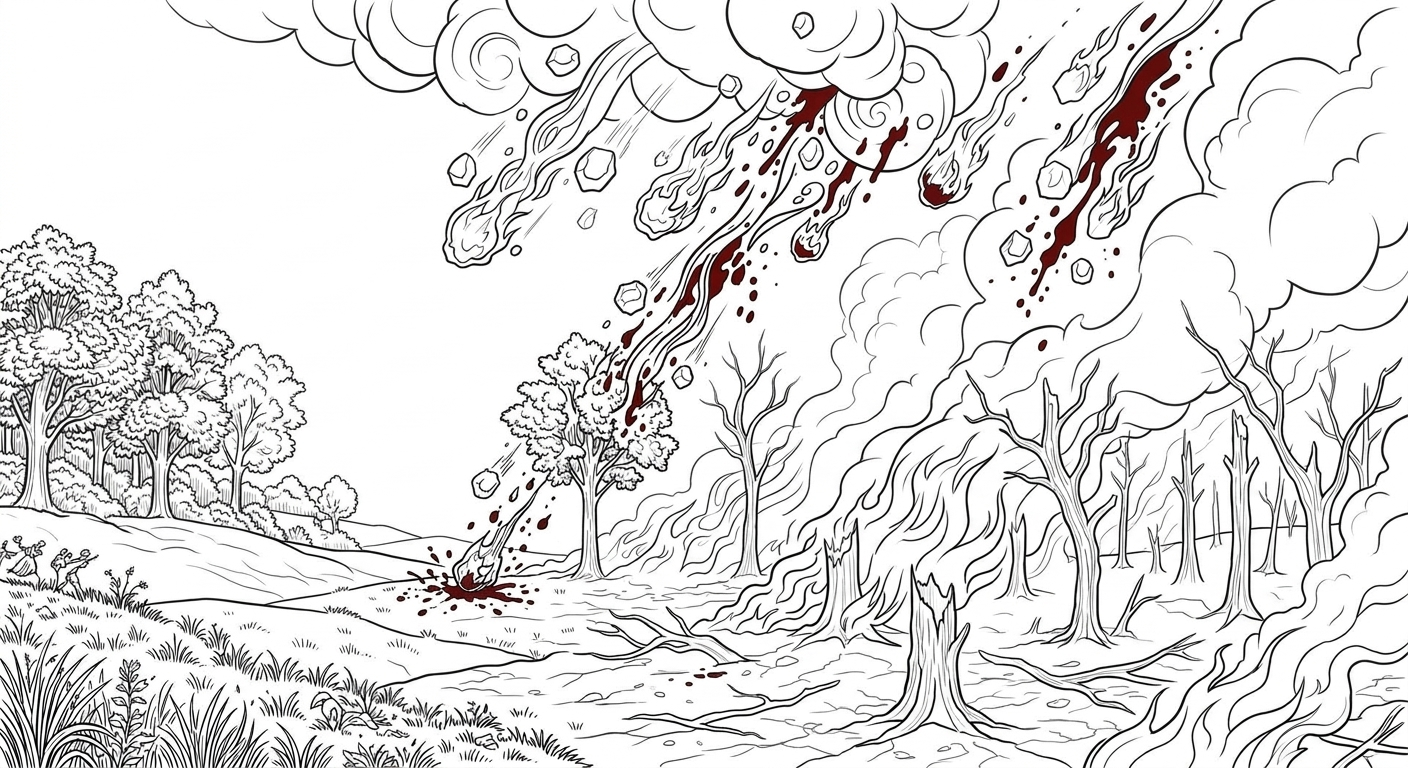
\includegraphics[
    width=1\textwidth,
    trim=0 0 0 0,
    clip]{images/trumpet_1st.jpg}
\end{figure}

At the sound of the first trumpet\index{trumpets, seven!1@first trumpet}, hail and fire mixed with blood are hurled upon the earth. A third of the earth is burned, along with a third of the trees and all the green grass.

The judgment begins with the land itself. What once nourished life is struck, and the familiar landscape becomes a scene of devastation. The green world, which bears witness to the Creator\index{Creator}'s generosity, now bears the marks of divine judgment. Yet the destruction is limited: a third is struck, not the whole.

\section{The Second Trumpet}\index{trumpets, seven!2@second trumpet}

\begin{ScriptureBox}

\item[8:8] The second angel sounded his trumpet, and something like a huge mountain, all ablaze, was thrown into the sea. A third of the sea turned into blood,

\item[8:9] a third of the living creatures in the sea died, and a third of the ships were destroyed.
% CHECK NIV: Revelation 8:8--9 supplied from memory, not from pasted text;
% verify wording against Bible Gateway (NIV 2011).

\end{ScriptureBox}

\begin{figure}[htbp]
    \centering
    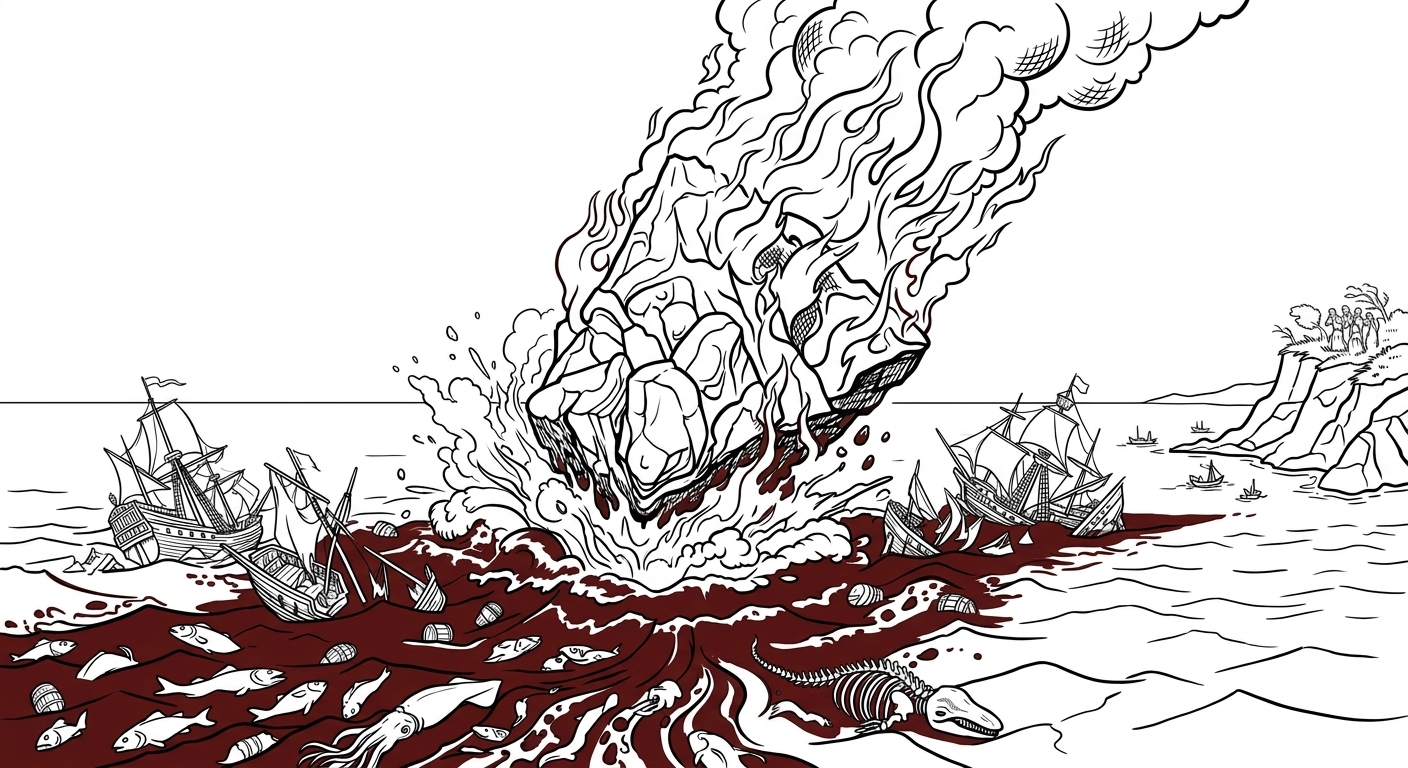
\includegraphics[
    width=1\textwidth,
    trim=0 0 0 0,
    clip]{images/trumpet_2nd.jpg}
\end{figure}

At the second trumpet\index{trumpets, seven!2@second trumpet}, something like a great mountain ablaze with fire is hurled into the sea. A third of the sea turns to blood, a third of its living creatures die, and a third of the ships are destroyed.

The sea, a source of food, commerce, and passage between distant lands, becomes a place of death and ruin. The destruction reaches beyond the shoreline, striking the creatures that inhabit the waters and the vessels that carry human life and trade across them. The judgment touches not only the natural world but also the networks upon which human civilization depends.

\section{The Third Trumpet}\index{trumpets, seven!3@third trumpet}

\begin{ScriptureBox}

\item[8:10] The third angel sounded his trumpet, and a great star, blazing like a torch, fell from the sky on a third of the rivers and on the springs of water---

\item[8:11] the name of the star is Wormwood. A third of the waters turned bitter, and many people died from the waters that had become bitter.
% NIV footnote for 8:11 (omitted; add as \footnote if wanted):
%   ``Wormwood'' --- Wormwood is a bitter substance.
% CHECK NIV: footnote wording quoted from memory; verify against Bible Gateway.

\end{ScriptureBox}

\begin{figure}[htbp]
    \centering
    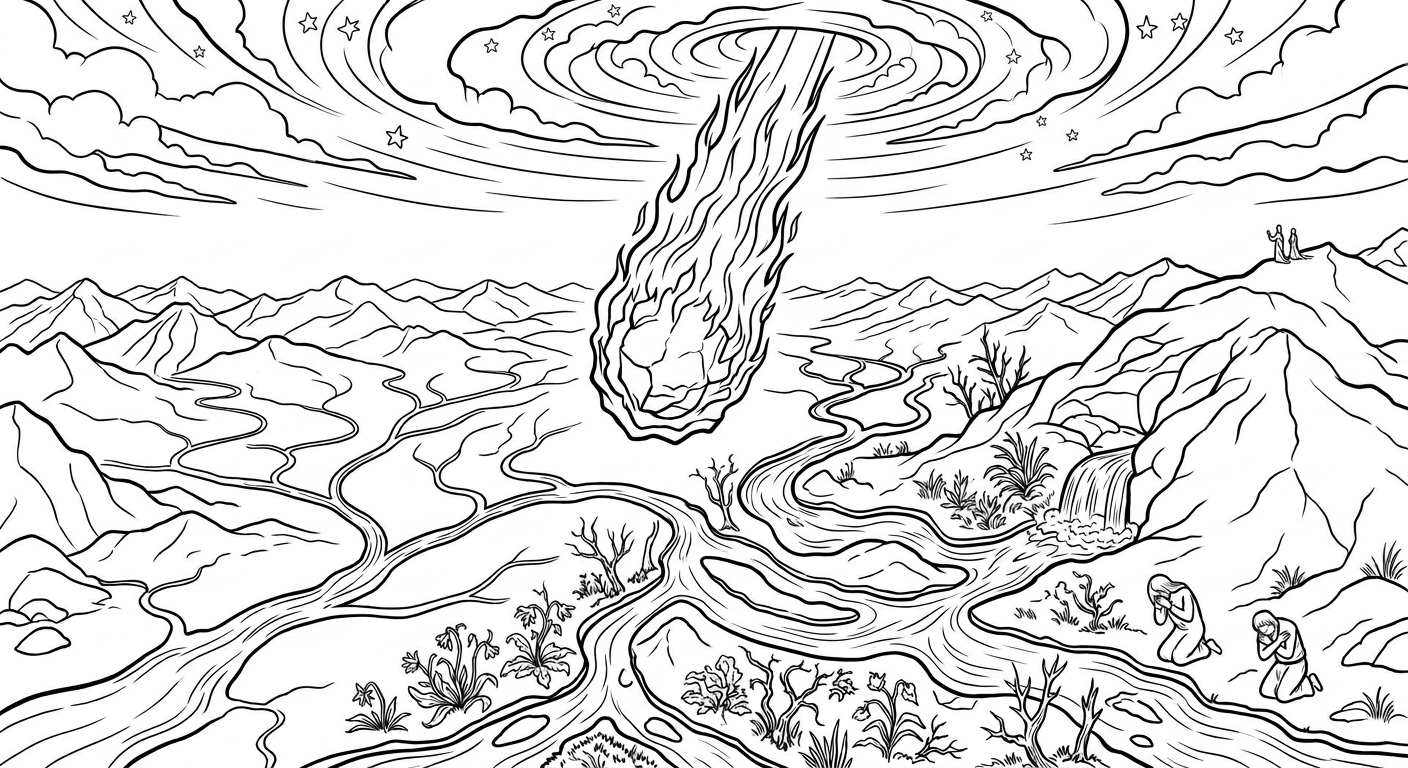
\includegraphics[
    width=1\textwidth,
    trim=0 0 0 0,
    clip]{images/trumpet_3rd.jpg}
\end{figure}

The star that falls from heaven is called Wormwood\index{Wormwood}. In Greek, the name is \textit{apsinthos}; in English, the plant is known as wormwood. It is associated with an intensely bitter taste. In the ancient world, wormwood was used for medicinal purposes and to repel insects; a related plant later became associated with the production of absinthe.

In the Old Testament, wormwood is often a symbol of bitterness, suffering, and judgment. Jeremiah 9:15, for example, declares that the people will be made to eat wormwood and drink poisoned water. Similar imagery appears in Lamentations 3:15 and Amos 5:7.

The vision in Revelation draws upon this established biblical imagery. When a third of the waters becomes wormwood, the emphasis falls on their bitter, undrinkable condition and the death that follows. Water, ordinarily a source of life, becomes an instrument of judgment. The very thing upon which human beings depend for survival is turned into a source of bitterness and death.

\section{The Fourth Trumpet}\index{trumpets, seven!4@fourth trumpet}

\begin{ScriptureBox}

% Insert the licensed NIV text of Revelation 8:12.
\item[8:12] \textit{The fourth angel sounded his trumpet, and a third of the sun was struck, a third of the moon, and a third of the stars, so that a third of them turned dark. A third of the day was without light, and also a third of the night.}

\end{ScriptureBox}

\begin{figure}[htbp]
    \centering
    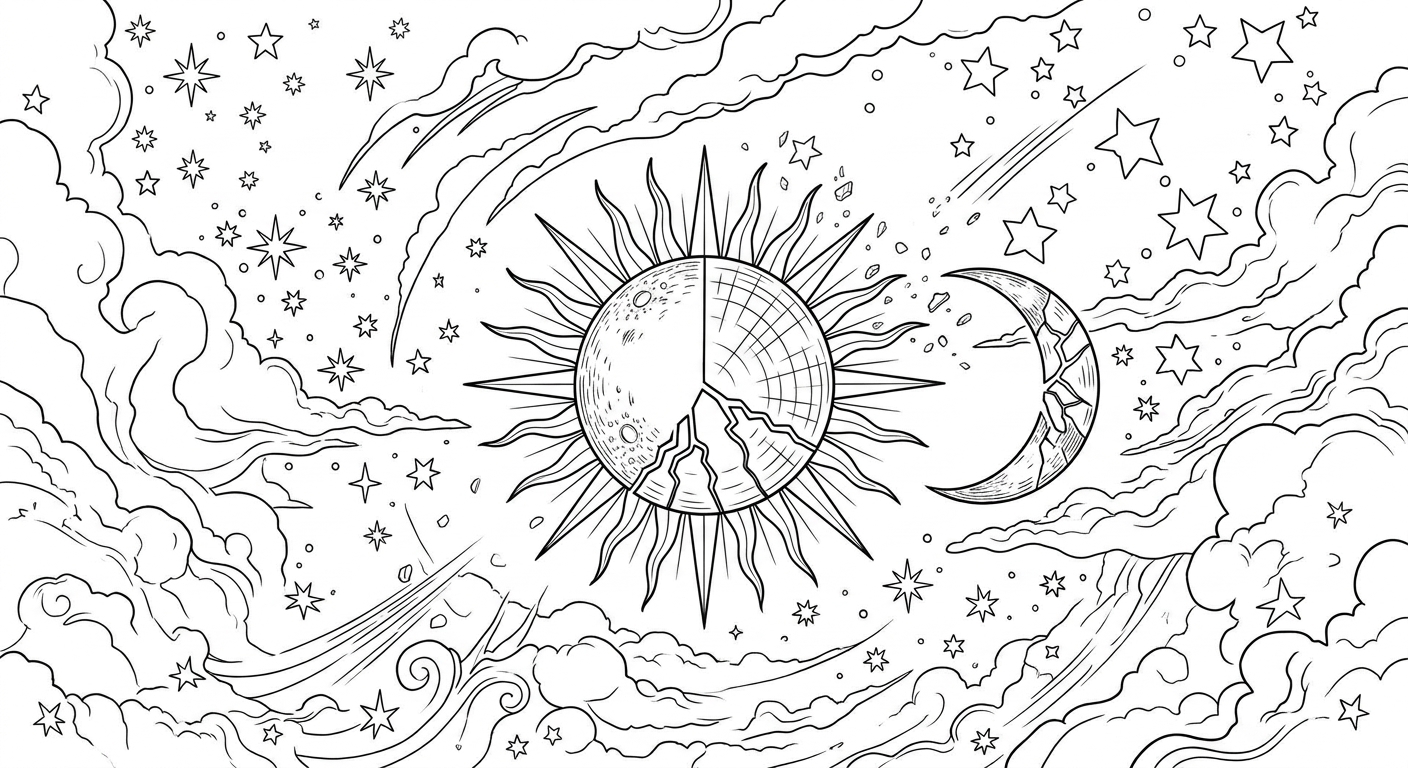
\includegraphics[
    width=1\textwidth,
    trim=0 0 0 0,
    clip]{images/trumpet_4th.jpg}
\end{figure}

At the fourth trumpet\index{trumpets, seven!4@fourth trumpet}, a third of the sun, moon, and stars is struck. A third of the day loses its light, and the night is darkened as well.

The rhythm of day and night, so familiar that humanity often takes it for granted, is disrupted. The lights that govern the heavens and mark the passage of time are darkened. The world below is left under a shadow that reaches from the earth to the sky.

The first four trumpets thus strike different parts of the created order: the land, the sea, the fresh waters, and the heavenly lights. Yet each judgment remains partial. The repeated limitation to a third is a sobering reminder that the devastation is real, but the final destruction has not yet come.

\section{The Fifth Trumpet}\index{trumpets, seven!5@fifth trumpet}

\begin{ScriptureBox}

\item[8:13] \textit{As I watched, I heard an eagle that was flying in midair call out in a loud voice: “Woe! Woe! Woe to the inhabitants of the earth, because of the trumpet blasts about to be sounded by the other three angels!”}

\item[9:1] The fifth angel sounded his trumpet, and I saw a star that had fallen from the sky to the earth. The star was given the key to the shaft of the Abyss.

\item[9:2] When he opened the Abyss, smoke rose from it like the smoke from a gigantic furnace. The sun and sky were darkened by the smoke from the Abyss.

\item[9:3] And out of the smoke locusts came down on the earth and were given power like that of scorpions of the earth.

\item[9:4] They were told not to harm the grass of the earth or any plant or tree, but only those people who did not have the seal of God on their foreheads.

\item[9:5] They were not allowed to kill them but only to torture them for five months. And the agony they suffered was like that of the sting of a scorpion when it strikes.

\item[9:6] During those days people will seek death but will not find it; they will long to die, but death will elude them.

\item[9:7] The locusts looked like horses prepared for battle. On their heads they wore something like crowns of gold, and their faces resembled human faces.

\item[9:8] Their hair was like women's hair, and their teeth were like lions' teeth.

\item[9:9] They had breastplates like breastplates of iron, and the sound of their wings was like the thundering of many horses and chariots rushing into battle.

\item[9:10] They had tails with stingers, like scorpions, and in their tails they had power to torment people for five months.

\item[9:11] They had as king over them the angel of the Abyss, whose name in Hebrew is Abaddon and in Greek is Apollyon (that is, Destroyer).

\item[9:12] The first woe is past; two other woes are yet to come.

\end{ScriptureBox}

\begin{figure}[htbp]
    \centering
    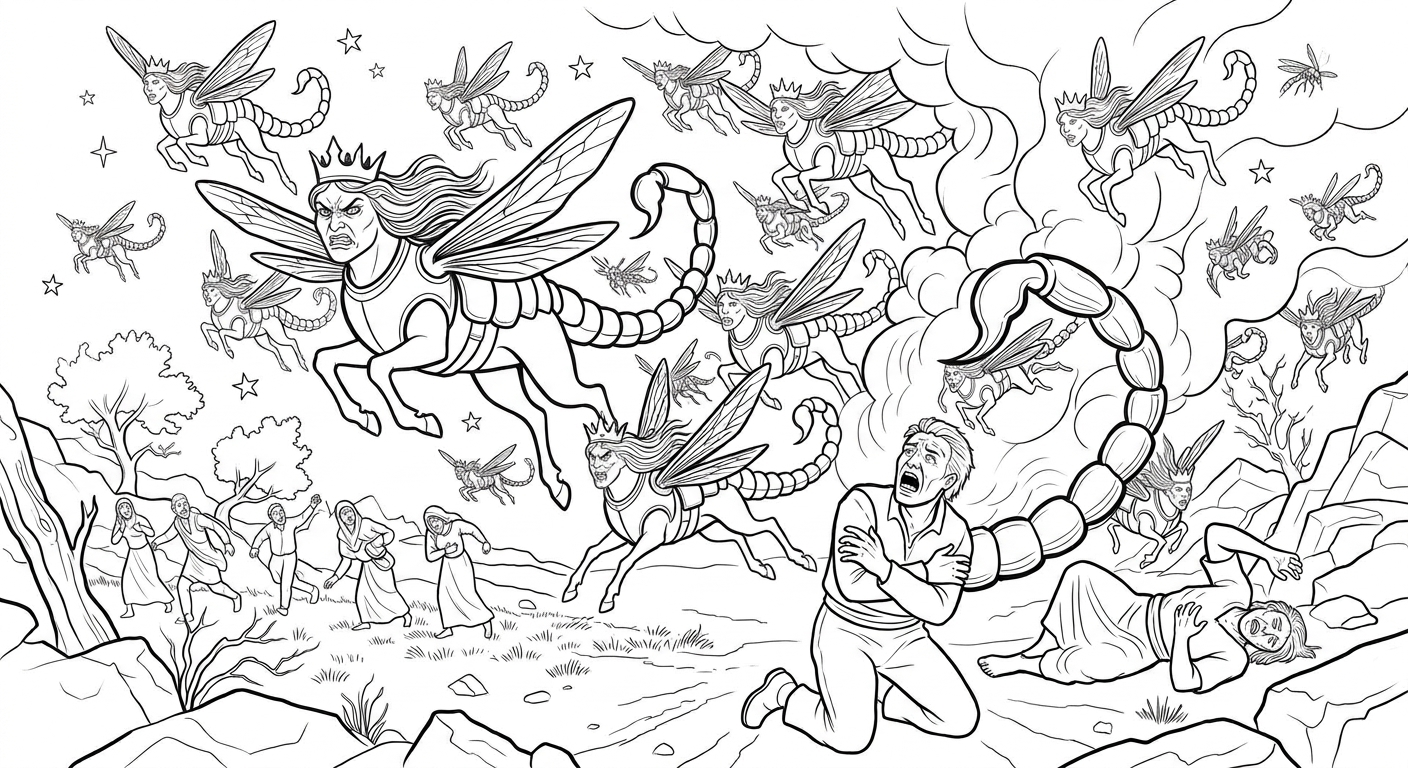
\includegraphics[
    width=1\textwidth,
    trim=0 0 0 0,
    clip]{images/trumpet_5th.jpg}
\end{figure}

As the first four trumpets fall silent, John sees an eagle flying overhead, proclaiming three woes\index{woes, three} upon the inhabitants of the earth. The remaining trumpets will bring judgments of a different and more terrifying kind. The first woe begins when the fifth angel sounds his trumpet.

A star has fallen from heaven to earth, and the key to the Abyss\index{Abyss} is given to it. When the Abyss is opened, smoke rises like the smoke of a great furnace, darkening the sun and the sky. Out of the smoke comes a swarm of locusts\index{locusts}, but these are no ordinary insects. They are granted power like that of scorpions, and their mission is unlike that of the locusts familiar to the world.

They are forbidden to harm the grass, plants, or trees. Instead, they are commanded to torment those who do not bear the seal of God on their foreheads. They cannot kill their victims, but for five months they inflict agony like the sting of a scorpion. The suffering is so severe that people long for death, yet death eludes them.

John describes the locusts\index{locusts} through a succession of startling comparisons. They resemble horses prepared for battle, wear something like crowns of gold, and have faces like human faces. Their hair is like women's hair, their teeth like lions' teeth, and their breastplates like iron. The sound of their wings resembles the thunderous rush of chariots and horses charging into battle. Their tails are like scorpions, armed with stingers that torment people for five months.

Their king is the angel of the Abyss\index{Abyss}, called Abaddon in Hebrew and Apollyon in Greek—names associated with destruction and the destroyer. The first woe has passed, but two more are still to come.

The vision is terrifying not merely because it depicts strange and dreadful creatures, but because it portrays a realm of judgment in which torment is permitted yet bounded. The locusts\index{locusts} can harm, but they cannot kill; their power is real, but it is limited. Even in the midst of this darkness, the vision continues to reveal that evil does not exercise unlimited authority.

\section{The Sixth Trumpet}\index{trumpets, seven!6@sixth trumpet}

\begin{ScriptureBox}

\item[9:13] The sixth angel sounded his trumpet, and I heard a voice coming from the four horns of the golden altar that is before God.

\item[9:14] It said to the sixth angel who had the trumpet, ``Release the four angels who are bound at the great river Euphrates.''

\item[9:15] And the four angels who had been kept ready for this very hour and day and month and year were released to kill a third of mankind.

\item[9:16] The number of the mounted troops was twice ten thousand times ten thousand. I heard their number.

\item[9:17] The horses and riders I saw in my vision looked like this: Their breastplates were fiery red, dark blue, and yellow as sulfur. The heads of the horses resembled the heads of lions, and out of their mouths came fire, smoke and sulfur.

\item[9:18] A third of mankind was killed by the three plagues of fire, smoke and sulfur that came out of their mouths.

\item[9:19] The power of the horses was in their mouths and in their tails; for their tails were like snakes, having heads with which they inflict injury.

\item[9:20] The rest of mankind who were not killed by these plagues still did not repent of the work of their hands; they did not stop worshiping demons, and idols of gold, silver, bronze, stone and wood---idols that cannot see or hear or walk.

\item[9:21] Nor did they repent of their murders, their magic arts, their sexual immorality or their thefts.

\end{ScriptureBox}

\begin{figure}[htbp]
    \centering
    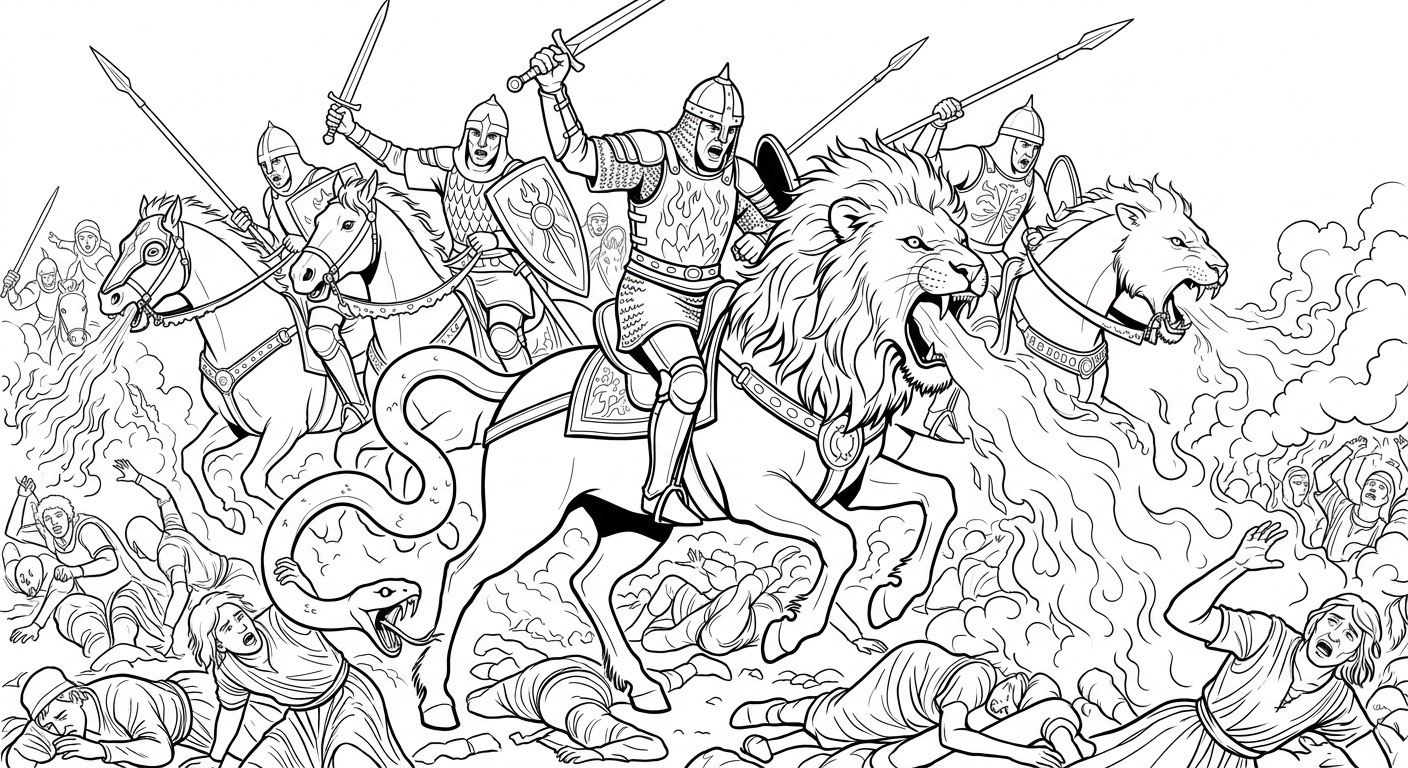
\includegraphics[
    width=1\textwidth,
    trim=0 0 0 0,
    clip]{images/trumpet_6th.jpg}
\end{figure}

When the sixth angel sounds his trumpet, a voice comes from the four horns of the golden altar\index{altar} before God. The angel is commanded to release the four angels bound at the great river Euphrates\index{Euphrates}. They have been kept ready for a precise moment—the appointed year, month, day, and hour—when they will kill a third of humanity.

The four angels command an army of two hundred million horsemen. John hears their number and then sees them in his vision. The riders wear breastplates the color of fire, sapphire, and sulfur. The horses have heads like lions, and fire, smoke, and sulfur pour from their mouths. These three plagues\index{plagues} kill a third of humanity. The horses' power lies in their mouths and tails; their tails resemble snakes, with heads that inflict harm.

The identity of the four bound angels is not made explicit. They may represent fallen angels or demonic powers held in restraint, though some interpreters have also considered historical military forces. The vision's emphasis, however, is clear: a vast and terrifying force is released to bring death upon humanity, and its activity unfolds under a divinely appointed limit.

The expression “two hundred million” is often understood in light of the Greek wording, which conveys the idea of an immense number—literally, “myriads of myriads.” The image emphasizes the overwhelming scale of the army; it need not be treated as a modern statistical report calculated by multiplying twenty thousand by twenty thousand.

The Euphrates\index{Euphrates} was an important geographical boundary to the northeast of ancient Israel\index{Israel}. It was also associated with the territory promised by God and with the threat of foreign powers advancing from the northeast.\footnote{When God made His covenant with Abraham, He promised his descendants territory extending from the river of Egypt to the Euphrates (Genesis 15:18). Isaiah, meanwhile, used the image of the Euphrates overflowing its banks to portray the might of the king of Assyria and his armies, whose power would sweep into Judah like a flood (Isaiah 8:7--8).} In Revelation, the judgment associated with this river reaches beyond the borders of ancient Israel and touches humanity on a vast scale.

One might expect a calamity of such magnitude to bring people to repentance\index{repentance}. Yet disaster does not, by itself, produce a repentant heart. This is one of the most sobering truths in the passage. Even after witnessing death and devastation, the survivors refuse to turn from the works of their hands. They continue to worship demons and lifeless idols made of gold, silver, bronze, stone, and wood—things that cannot see, hear, or walk. They also refuse to repent of their murders, sorceries, sexual immorality, and theft.

The tragedy is not merely that humanity suffers judgment. It is that humanity persists in rebellion even while judgment unfolds before its eyes. The human heart can witness devastation and still cling to the very sins that lead to ruin.

\begin{ReaderQuestion}
Revelation 9:20--21 emphasizes that people still refuse to repent even after experiencing devastating judgments. Why do suffering and disaster not necessarily lead people to repentance? What does this passage teach us about the nature of repentance and the human heart?
\end{ReaderQuestion}

Once again, the repeated limitation to a third deserves attention. The judgments of the trumpets are severe, but they do not yet consume the whole created order. The world is struck, but not wholly destroyed. The restraint is significant: judgment has come, yet the vision has not reached the final end of all things.

\begin{figure}[htbp]
    \centering
    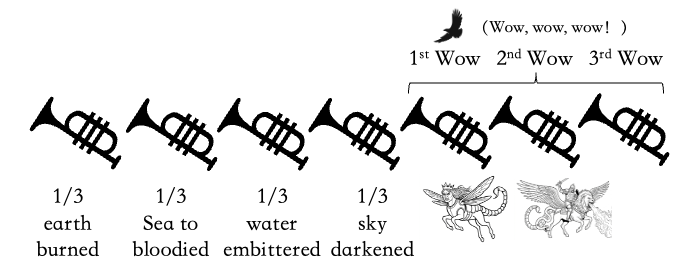
\includegraphics[
    width=1\textwidth,
    trim=0 0 0 0,
    clip]{images/trumpets_woes.png}
    \caption{The Seven Trumpets}
    \label{fig:trumpets_woes}
\end{figure}

\section{Future Events, Ancient Language}

You may have noticed that God allows John to describe these visions through images familiar to people of the first century: horses, cavalry, and the weapons of ancient warfare. Yet modern warfare no longer depends on horses and swords. It employs drones, fighter jets, missiles, and increasingly sophisticated military technologies. The wars of the future may involve technologies beyond anything we can presently imagine.

If the visions in Revelation concern future events, why does John describe them in terms of horses and ancient weapons? Why did God not simply show John the military technology of the future and enable him to describe it directly? Some readers have even suggested that the horses must be tanks, the fire must be missiles, or the locusts\index{locusts} must be helicopters.

A more careful answer is that God's purpose is not to give John a preview of future weapons technology. His purpose is to reveal His judgment and sovereignty. Seeing a future technology would not necessarily mean understanding the revelation God intended to communicate. God gave John visions in a form he could describe to the people of his own time, while preserving their significance for readers in generations to come.

Consider Revelation 9:7, which says that the locusts\index{locusts} looked like horses prepared for battle. Revelation 9:17 describes horses with heads like lions, and verse 19 compares their tails to snakes. John does not simply say, “I saw horses.” Again and again, he reaches for the words “like” and “as” to convey what he sees. His language is the language of comparison, attempting to express a vision that exceeds ordinary experience.

Imagine, for a moment, that God had shown John an F-35 fighter jet. How might a man of the first century have described it? He might have written, “I saw an enormous iron bird with two wings, breathing fire as it flew across the sky.” Such a description might sound strange to a modern reader, but it would be a natural attempt to convey an unfamiliar sight using familiar language.

Throughout Revelation, words such as “like” and “as” remind us that John is describing extraordinary visions through the language available to him. We should therefore be cautious about translating the imagery directly into modern military hardware, such as Apache helicopters or contemporary tanks. Such identifications may seem compelling in one generation and become obsolete in the next. More importantly, they can distract us from the theological message of the vision.\footnote{See G. K. Beale (1999) and Richard Bauckham (1993).}

There is another reason to resist reducing these images to modern technology: Revelation is deeply rooted in the language and imagery of the Old Testament. The locusts\index{locusts} in Revelation 9, for example, strongly recall Joel's prophecy of the day of the Lord\index{day of the Lord}. Joel 2:4 describes the locusts this way: “They have the appearance of horses; they gallop along like cavalry” (NIV).

Readers familiar with Israel\index{Israel}'s Scriptures would recognize this language and recall the prophetic themes associated with the day of the Lord\index{day of the Lord}, divine judgment, and the end of the age. The imagery in Revelation is not merely a coded description of some future weapon. It draws the reader into the larger biblical story of God's judgment against evil and His ultimate rule over history.

If John had instead described an F-35, his readers might have struggled to understand the image, and the connection to Joel's prophecy would have been obscured. By using the language of Scripture, the vision speaks across generations. Its central message does not depend on our ability to identify a particular machine or predict a particular military event. It calls us to recognize the seriousness of divine judgment, the limits of human power, and the need to turn to God in repentance\index{repentance}.

The eagle's task is therefore not to gaze into the vision merely to identify the machinery of war, but to look beyond the terrifying images and discern the truth they reveal: history remains under God's sovereign hand, judgment is real, and humanity's greatest need is not technological understanding but a heart willing to repent.

\chapter{Faithful Witnesses in the Midst of Suffering (10:1--11:19)}

In the previous chapter, we read about the first six trumpets. Surely, the seventh trumpet\index{trumpets, seven!7@seventh trumpet} must be next. Yet before it sounds, Revelation pauses to present two visions: John is commissioned to prophesy again, and two witnesses\index{two witnesses} testify before the world. Only then does the seventh trumpet sound.

Why are these two visions placed here? Both reveal an essential truth: even as God's judgments\index{judgment} unfold, His people still bear the responsibility of witnessing to Him. Though suffering and persecution\index{persecution} may come, they are called to remain faithful to His Word and to testify to His truth until the kingdom of Christ is fully revealed.

From the heights, the eagle sees not only the judgments falling upon the earth, but also the witnesses who continue to proclaim God's truth amid the gathering darkness. Judgment does not silence their calling. Rather, their faithfulness shines all the more clearly against the shadows of a world opposed to God.

\section{John Is Commissioned to Prophesy Again}
\begin{ScriptureBox}

\item[10:1] Then I saw another mighty angel coming down from heaven. He was robed in a cloud, with a rainbow above his head; his face was like the sun, and his legs were like fiery pillars.

\item[10:2] He was holding a little scroll, which lay open in his hand. He planted his right foot on the sea and his left foot on the land,

\item[10:3] and he gave a loud shout like the roar of a lion. When he shouted, the voices of the seven thunders spoke.

\item[10:4] And when the seven thunders spoke, I was about to write; but I heard a voice from heaven say, ``Seal up what the seven thunders have said and do not write it down.''

\item[10:5] Then the angel I had seen standing on the sea and on the land raised his right hand to heaven.

\item[10:6] And he swore by him who lives for ever and ever, who created the heavens and all that is in them, the earth and all that is in it, and the sea and all that is in it, and said, ``There will be no more delay!

\item[10:7] But in the days when the seventh angel is about to sound his trumpet, the mystery of God will be accomplished, just as he announced to his servants the prophets.''

\item[10:8] Then the voice that I had heard from heaven spoke to me once more: ``Go, take the scroll that lies open in the hand of the angel who is standing on the sea and on the land.''

\item[10:9] So I went to the angel and asked him to give me the little scroll. He said to me, ``Take it and eat it. It will turn your stomach sour, but `in your mouth it will be as sweet as honey.'\,''
% NIV footnote for 10:9 (omitted; add as \footnote if wanted):
%   ``as sweet as honey'' --- Ezek. 3:3
% CHECK NIV: footnote reference quoted from memory; verify against Bible Gateway.

\item[10:10] I took the little scroll from the angel's hand and ate it. It tasted as sweet as honey in my mouth, but when I had eaten it, my stomach turned sour.

\item[10:11] Then I was told, ``You must prophesy again about many peoples, nations, languages and kings.''

\end{ScriptureBox}


\begin{figure}[htbp]
    \centering
    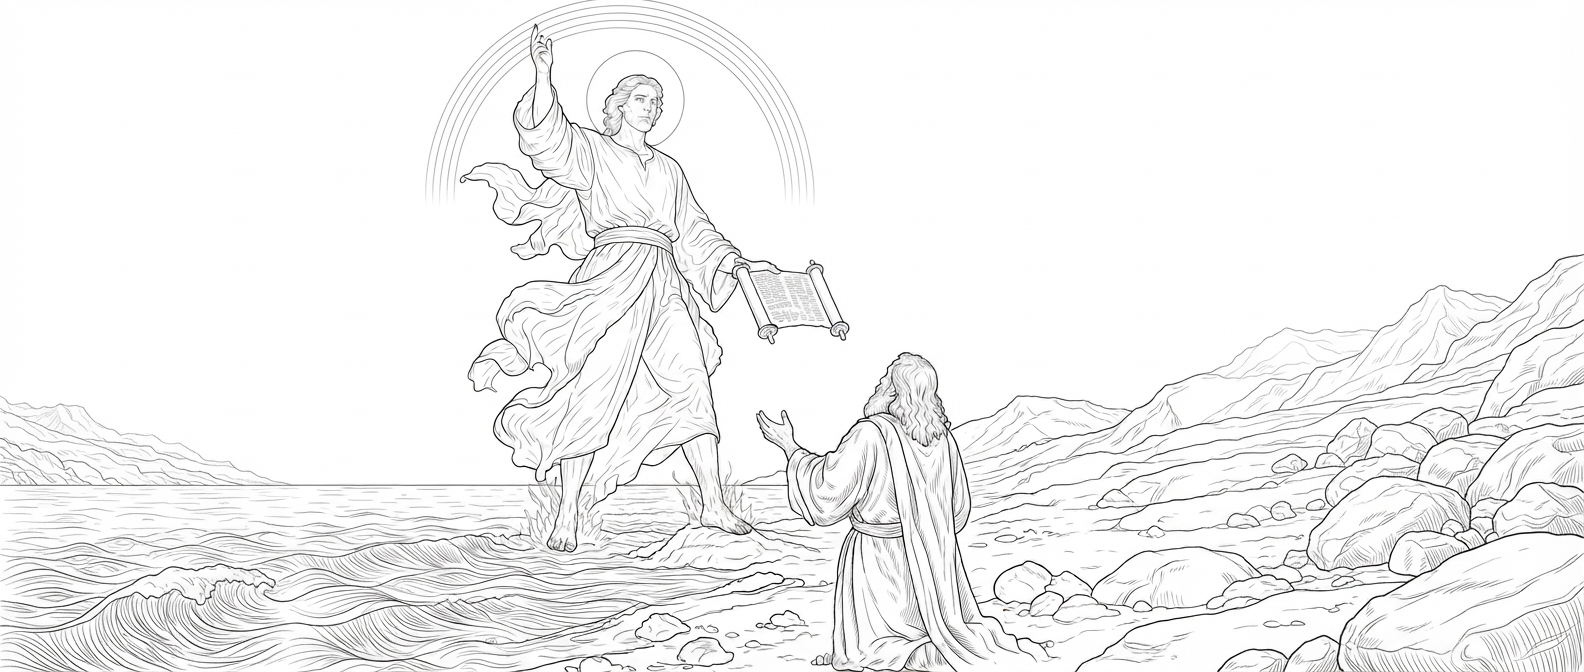
\includegraphics[
    width=1\textwidth,
    trim=200 0 200 0,
    clip]{images/small_scroll2.jpg}
\end{figure}

God's Word is sweet as honey in the mouth because it reveals His truth and brings comfort to those who receive it. Yet the same Word turns bitter in John's stomach, for proclaiming God's truth faithfully also means confronting judgment, suffering, and persecution\index{persecution}.

The sweetness and bitterness belong together. God's revelation is a gift, illuminating the darkness and offering hope to His people. But the messenger who receives that gift must also bear the burden of proclaiming it. The truth that comforts the faithful may expose the world's rebellion and provoke the hostility of those who refuse to hear it.

\begin{ReaderQuestion}
Why is God's Word both “sweet as honey” and bitter in the stomach? What does this image teach us about the joy and the cost of receiving and proclaiming God's truth?
\end{ReaderQuestion}

When John prepares to write down what the seven thunders have spoken, a voice from heaven commands him to seal up their words and not write them down. Not everything John hears or sees is to be disclosed. God determines what is revealed and what remains hidden.

Deuteronomy 29:29 expresses this principle: “The secret things belong to the LORD our God, but the things revealed belong to us and to our children forever” (NIV).

The heart of our faith does not lie in discovering every detail of the end times\index{end times}. It lies in trusting the God who governs history and faithfully receiving the truth He has chosen to reveal. There is a spiritual discipline in acknowledging the limits of our understanding. We are called to approach what remains hidden with humility and to devote ourselves to obeying what God has already made known.

John is then commanded to take the little scroll\index{scroll!little scroll} and eat it. Its sweetness and bitterness prepare him for the work that follows: he must prophesy again concerning many peoples, nations, languages, and kings. Receiving God's Word is not the end of his calling. He must carry that Word into the world, whatever the cost.

So it is with God's people in every generation. We do not receive His Word merely to satisfy our curiosity or comfort ourselves in private. We receive it so that we may live by it, proclaim it, and remain faithful to it—even when obedience brings sorrow.

\section{The Two Witnesses}\index{two witnesses}
\begin{ScriptureBox}

\item[11:1] I was given a reed like a measuring rod and was told, ``Go and measure the temple of God and the altar, with its worshipers.

\item[11:2] But exclude the outer court; do not measure it, because it has been given to the Gentiles. They will trample on the holy city for 42 months.

\item[11:3] And I will appoint my two witnesses, and they will prophesy for 1,260 days, clothed in sackcloth.''

\item[11:4] They are ``the two olive trees'' and the two lampstands, and ``they stand before the Lord of the earth.''
% NIV footnote for 11:4 (omitted; add as \footnote if wanted):
%   ``before the Lord of the earth'' --- Zech. 4:3,11,14
% CHECK NIV: footnote reference quoted from memory; verify against Bible Gateway.

\item[11:5] If anyone tries to harm them, fire comes from their mouths and devours their enemies. This is how anyone who wants to harm them must die.

\item[11:6] They have power to shut up the heavens so that it will not rain during the time they are prophesying; and they have power to turn the waters into blood and to strike the earth with every kind of plague as often as they want.

\item[11:7] Now when they have finished their testimony, the beast that comes up from the Abyss will attack them, and overpower and kill them.

\item[11:8] Their bodies will lie in the public square of the great city---which is figuratively called Sodom and Egypt---where also their Lord was crucified.

\item[11:9] For three and a half days some from every people, tribe, language and nation will gaze on their bodies and refuse them burial.

\item[11:10] The inhabitants of the earth will gloat over them and will celebrate by sending each other gifts, because these two prophets had tormented those who live on the earth.

\item[11:11] But after the three and a half days the breath of life from God entered them, and they stood on their feet, and terror struck those who saw them.
% NIV footnote for 11:11 (omitted; add as \footnote if wanted):
%   ``breath'' --- Or Spirit (see Ezek. 37:5,14)
% CHECK NIV: footnote wording quoted from memory; verify against Bible Gateway.

\item[11:12] Then they heard a loud voice from heaven saying to them, ``Come up here.'' And they went up to heaven in a cloud, while their enemies looked on.

\item[11:13] At that very hour there was a severe earthquake and a tenth of the city collapsed. Seven thousand people were killed in the earthquake, and the survivors were terrified and gave glory to the God of heaven.

\end{ScriptureBox}

\subsection{The Temple Is Measured, and the Holy City Is Trampled}\index{holy city}\index{temple}

Biblical visions sometimes depict the measuring of a temple\index{temple} or a city. Ezekiel\index{Ezekiel} 40--48 describes the measuring of the temple, while Zechariah\index{Zechariah} 2:1--5 records a vision in which Jerusalem\index{Jerusalem} is measured. Such imagery can signify God's recognition of what belongs to Him, its distinction as holy, and His protective claim over it.

In Revelation 11, John is told to measure God's temple, the altar\index{altar}, and those who worship\index{worship} there. The outer court, however, is excluded from the measurement and handed over to the Gentiles, who will trample the holy city\index{holy city} for forty-two months.

The image holds two truths together. God's people belong to Him, yet they may still suffer persecution\index{persecution} on earth. Being known by God does not mean being spared every trial. His people may be oppressed, their worship challenged, and their witness resisted, even as they remain His own.

How long will this oppression last? Several visions in Scripture use periods of time that correspond to one another: “forty-two months” (Revelation 11:2), “1,260 days\index{1,260 days}” (Revelation 11:3), and “a time, times and half a time\index{time, times, and half a time}” (Revelation 12:14). If a year is reckoned as twelve months of thirty days each, these expressions correspond to three and a half years.

Christian interpreters differ over how these periods should be understood and applied. Some read them as specific future periods, while others interpret them symbolically or in relation to the wider history of God's people. I discuss these views in the appendix, “How Long Will the Great Tribulation\index{Great Tribulation} Last? The Seventy Sevens\index{seventy sevens (Daniel 9)} of Daniel\index{Daniel}.”

Whatever interpretive approach one adopts, the period is significant in one essential respect: the time of suffering is limited. The forces that oppose God do not possess unlimited authority. The holy city\index{holy city} may be trampled, and the witnesses may be attacked, but their enemies cannot determine the final course of history. Their time is bounded by the sovereignty of God.

\begin{figure}[htbp]
    \centering
    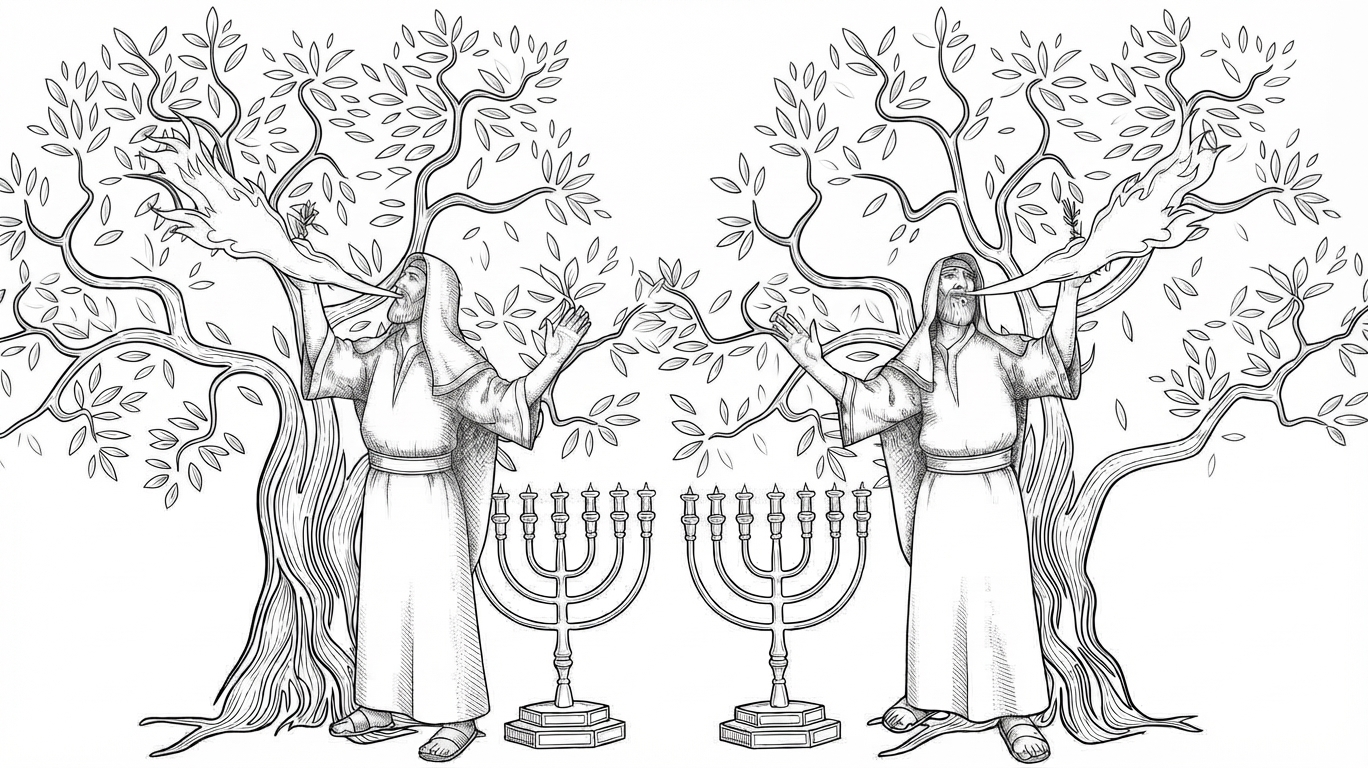
\includegraphics[
    width=1\textwidth,
    trim=0 0 0 0,
    clip]{images/two_witnesses.jpg}
\end{figure}

\subsection{Who Are the Two Witnesses?}\index{two witnesses}

John's vision draws extensively upon the Old Testament. Recognizing these connections helps us understand both the imagery and the theological meaning of the two witnesses\index{two witnesses}, as shown in Table \ref{tab:rev11-ot-background}.

{
\small
\renewcommand{\arraystretch}{1}

\begin{longtable}{
    @{}
    >{\raggedright\arraybackslash}p{0.24\textwidth} |
    >{\raggedright\arraybackslash}p{0.26\textwidth} |
    >{\raggedright\arraybackslash}p{0.40\textwidth}
    @{}
}
\caption{Old Testament background to Revelation 11}
\label{tab:rev11-ot-background} \\
\hline
\textbf{Revelation 11} & \textbf{Old Testament} & \textbf{Significance} \\
\hline
\endfirsthead

\multicolumn{3}{@{}l}{\small\itshape Table~\thetable\ (continued)} \\
\hline
\textbf{Revelation 11} & \textbf{Old Testament} & \textbf{Significance} \\
\hline
\endhead

\hline
\endfoot

\hline
\endlastfoot

The two witnesses
& Deuteronomy 19:15
& The principle that a matter is established by two or three witnesses \\
\hline
The two olive trees
& Zechariah 4:1--14
& The olive trees and lampstand in Zechariah's vision \\
\hline
The two lampstands
& Zechariah 4; Revelation 1:20
& Witness and the people of God \\
\hline
Fire from their mouths
& Jeremiah 5:14
& The power of God's word to pronounce judgment \\
\hline
The heavens shut
& 1 Kings 17:1
& Elijah's proclamation of drought \\
\hline
Water turned to blood
& Exodus 7:14--25
& Moses and the first plague upon Egypt \\
\hline
Various plagues
& Exodus
& The plagues through which God judged Egypt \\
\hline
The beast from the Abyss
& Daniel 7
& Political power in opposition to God \\
\hline
Sodom and Egypt
& Genesis; Exodus
& A corrupt and oppressive world that resists God and persecutes His people \\
\hline
Resurrection
& Ezekiel 37
& God's power to restore life to the dead \\
\hline
Taken up to heaven in a cloud
& Daniel 7:13; 2 Kings 2
& Divine glory and being taken up into heaven \\

\end{longtable}
}

\normalsize

These Old Testament connections provide a foundation for considering the different interpretations proposed by biblical scholars. The identity of the two witnesses\index{two witnesses} has been understood in several ways, as shown in Table \ref{tab:two-witnesses}.

{
\small
\renewcommand{\arraystretch}{1}

\begin{longtable}{
    @{}
    >{\raggedright\arraybackslash}p{0.35\textwidth} |
    >{\raggedright\arraybackslash}p{0.61\textwidth}
    @{}
}
\caption{Who are the two witnesses?}
\label{tab:two-witnesses} \\
\hline
\textbf{Proposed Identity} & \textbf{Principal Reasons} \\
\hline
\endfirsthead

\multicolumn{2}{@{}l}{\small\itshape Table~\thetable\ (continued)} \\
\hline
\textbf{Proposed Identity} & \textbf{Principal Reasons} \\
\hline
\endhead

\hline
\endfoot

\hline
\endlastfoot

Enoch and Elijah
& Both are described in Scripture as having been taken by God without an account of their ordinary deaths. \\
\hline
Moses and Elijah
& The signs involving fire, drought, and plagues recall the ministries of Elijah and Moses. Both also appear together at the Transfiguration of Jesus.\footnote{See the commentaries by Grant R. Osborne and John MacArthur.} \\
\hline
Two actual individuals raised up by God in the end times
& The detailed sequence of their preaching, death, resurrection, and ascent to heaven is understood as describing two specific future witnesses.\footnote{This view is held by a number of premillennial interpreters, including John MacArthur.} \\
\hline
The faithful church and people of God
& The imagery of the olive trees and lampstands is interpreted symbolically, representing the church's witness to the world.\footnote{See G. K. Beale and Craig R. Koester.} \\

\end{longtable}
}


\normalsize

These interpretations differ, but they all seek to account for the Old Testament imagery and the role of the witnesses in God's unfolding plan. The text does not explicitly name the two witnesses\index{two witnesses}, so it is wise to distinguish what the vision states directly from the conclusions interpreters draw from it.

Whatever their precise identity, their calling is unmistakable: they bear witness to God in a world that resists His truth. Their prophetic ministry recalls Moses\index{Moses} and Elijah\index{Elijah}, while the lampstand\index{lampstands} imagery connects their witness with the people of God. They proclaim the truth, confront evil, and remain faithful until their appointed testimony is complete.

Their story also overturns the world's measure of victory. The beast\index{beast} appears to prevail when it kills them, and the inhabitants of the earth celebrate their deaths. Yet the beast's triumph is temporary. God restores the witnesses to life and calls them into heaven. What appears to be defeat in the eyes of the world cannot overturn God's purpose.

\begin{ReaderQuestion}
The two witnesses are killed by the beast, and the inhabitants of the earth rejoice over their deaths. Today, might we also be tempted to remain silent about our faith because we fear how others will react? What can help us remain faithful to Christ?
\end{ReaderQuestion}

\subsection{What Do the Second and Third Woes Include?}\index{woes, three}

\begin{ScriptureBox}

% Insert the licensed NIV text of Revelation 11:14.
\item[11:14] \textit{The second woe has passed; the third woe is coming soon.}

\end{ScriptureBox}

The second woe\index{woes, three} encompasses the judgment associated with the sixth trumpet\index{trumpets, seven!6@sixth trumpet}, together with the vision of the two witnesses\index{two witnesses}. The third woe begins with the sounding of the seventh trumpet\index{trumpets, seven!7@seventh trumpet}. See Figure~\ref{fig:trumpets_woes}.

This transition reminds us that the visions in Revelation are not simply a sequence of disasters. Between the trumpets, John is shown the calling and suffering of God's witnesses. The judgments reveal God's opposition to evil, while the witnesses reveal the faithfulness He calls forth from His people. Even as the world is shaken, the testimony of God continues.

\section{The Seventh Trumpet Sounds}\index{trumpets, seven!7@seventh trumpet}

\begin{ScriptureBox}

\item[11:15] The seventh angel sounded his trumpet, and there were loud voices in heaven, which said:\\
\hspace*{1em}``The kingdom of the world has become\\
\hspace*{2em}the kingdom of our Lord and of his Messiah,\\
\hspace*{2em}and he will reign for ever and ever.''

\item[11:16] And the twenty-four elders, who were seated on their thrones before God, fell on their faces and worshiped God,

\item[11:17] saying:\\
\hspace*{1em}``We give thanks to you, Lord God Almighty,\\
\hspace*{2em}the One who is and who was,\\
\hspace*{1em}because you have taken your great power\\
\hspace*{2em}and have begun to reign.

\item[11:18] \hspace*{1em}The nations were angry,\\
\hspace*{2em}and your wrath has come.\\
\hspace*{1em}The time has come for judging the dead,\\
\hspace*{2em}and for rewarding your servants the prophets\\
\hspace*{1em}and your people who revere your name,\\
\hspace*{2em}both great and small---\\
\hspace*{1em}and for destroying those who destroy the earth.''

\item[11:19] Then God's temple in heaven was opened, and within his temple was seen the ark of his covenant. And there came flashes of lightning, rumblings, peals of thunder, an earthquake and a severe hailstorm.

\end{ScriptureBox}

When the seventh trumpet\index{trumpets, seven!7@seventh trumpet} sounds, heaven's first announcement is not another description of disaster. It is a proclamation of the certainty of Christ's reign: the kingdom of the world has become the kingdom of our Lord and of His Messiah\index{Messiah}, and He will reign for ever and ever.

The twenty-four elders\index{twenty-four elders} fall facedown before God in worship. They give thanks to the Lord God Almighty, who has taken His great power and begun to reign. The nations have raged, but God's wrath\index{wrath of God} has come. The time has arrived to judge the dead, to reward His servants the prophets and His holy people—all who fear His name, both great and small—and to destroy those who destroy the earth.

The seventh trumpet\index{trumpets, seven!7@seventh trumpet} therefore turns our attention beyond the partial judgments that have marked the earlier trumpets. The repeated limitation to a third gives way to the announcement of God's final purpose: evil will be judged, His faithful servants will be rewarded, and His reign will be openly established.

The opening of God's heavenly temple\index{temple} and the appearance of the ark of His covenant deepen this vision. The ark recalls God's covenant faithfulness and His presence among His people. Even amid lightning, rumblings, thunder, an earthquake\index{earthquake}, and a great hailstorm, the covenant-keeping God remains at the center of the vision.

The seventh trumpet\index{trumpets, seven!7@seventh trumpet} announces the certainty of the kingdom, though Revelation will continue to unfold the events and visions surrounding the final conflict. In the next chapter, we will look more deeply into the spiritual nature of that conflict and see how the powers that oppose God move toward their ultimate defeat.

The message to the church is clear: remain faithful in the midst of suffering. The witnesses may be despised, attacked, and even killed, but their testimony is not in vain. The beast\index{beast} does not have the final word. Christ does. The kingdom of the world will not remain forever in the hands of those who resist God; it belongs to the Lord and His Messiah\index{Messiah}, whose reign endures for ever and ever.

\begin{ReaderQuestion}
If God is calling you to be a faithful witness in your family, church, workplace, or circle of friends, what might He be asking you to uphold, change, or speak about with courage?
\end{ReaderQuestion}

\chapter{The Dragon and the Beasts: The Victory of the Lamb (12:1--14:20)}\index{dragon}\index{Lamb, the}

Revelation 12 and 13 draw extensively upon the visions and imagery of Genesis and Daniel\index{Daniel}. If we overlook these Old Testament backgrounds, we may be tempted to interpret the visions according to our own imaginations and, in doing so, misunderstand their meaning. This chapter therefore invites readers to return to the Old Testament, explore the roots of these symbols, and discover the spiritual conflict Revelation portrays: the struggle between the powers opposed to God and His unfolding plan of redemption\index{redemption}.

Why, then, can God's people overcome\index{overcomers} the devil? Revelation 12:11 gives us the answer: they overcome him “by the blood of the Lamb\index{Lamb, the!blood of} and by the word of their testimony.” The Christian struggle involves more than the people and circumstances we can see; beneath the visible world lies a deeper spiritual battle. The church does not conquer the dragon\index{dragon} through its own strength. Its victory rests upon the blood of the Lamb and upon a faithful testimony that endures even in suffering.

Chapter 14 then lifts our gaze to heaven, where angels proclaim the eternal gospel\index{eternal gospel} and call the inhabitants of the earth to fear God and give Him glory\index{glory}. Why, even at this late hour, does God still send His angels to proclaim the gospel?

What can endure beyond this fleeting earthly life?

The answer is found in receiving God's abundant grace\index{grace} and faithfully following Christ. To labor for the Lord, bear witness to Him, and nurture disciples while we remain on earth is itself a blessing. As Revelation 14:13 declares, those who die in the Lord are blessed, for their deeds follow them. These words remind us that our labor for Christ is never in vain. Even when believers endure suffering, they can persevere in faith, sustained by the hope that their faithful service will not be forgotten.

To help readers grasp the background and meaning of these visions without losing sight of the central theme—the victory of the Lamb\index{Lamb, the}—I have prepared the following table. It provides an overview of the visions, their Old Testament foundations, and their symbolic significance.

{
\small
\renewcommand{\arraystretch}{1}
\setlength{\tabcolsep}{4pt}

\begin{longtable}{
  >{\raggedright\arraybackslash}p{0.21\textwidth}
  >{\raggedright\arraybackslash}p{0.25\textwidth}
  >{\raggedright\arraybackslash}p{0.39\textwidth}
}
\caption{Old Testament background to the visions of Revelation 12--13}
\label{tab:rev12-13-ot-background} \\
\hline
Vision in Revelation &
Old Testament Background &
Symbolic Significance\\
\hline
\endfirsthead

\multicolumn{3}{l}{\small\itshape Table~\thetable\ (continued)} \\
\hline
Vision in Revelation &
Old Testament Background &
Symbolic Significance\\
\hline
\endhead

\hline
\endfoot

\hline
\endlastfoot

The woman &
Gen. 37:9--11; Isa. 54:1--8; 66:7--9 &
Israel and God's covenant people \\

The dragon &
Gen. 3:1--15 &
The ancient serpent, Satan, and the powers opposed to God \\

Seven heads and ten horns &
Dan. 7:7--8, 24 &
The imperial powers that oppose God \\

The male child &
Ps. 2:7--9 &
Jesus Christ, the Messianic King \\

The iron scepter &
Ps. 2:9 &
The Messiah's rule over the nations \\

1,260 days, forty-two months, and three and a half years &
Dan. 7:25; 12:7 &
A limited period of suffering; the powers opposed to God remain under His restraint \\

The war in heaven &
Dan. 10:13, 20--21; 12:1 &
The spiritual conflict taking place in the heavenly realm \\

The beast from the sea &
Dan. 7:2--8 &
Imperial power opposed to God and His people \\

The ten horns &
Dan. 7:7, 24 &
Political power exercised by kings \\

The beast from the earth &
Dan. 7; Rev. 13:11 &
A power that resembles the Lamb outwardly but speaks with the dragon's authority, deceiving the world \\

The mark on the forehead and hand &
Ex. 13:9, 16; Deut. 6:8; 11:18 &
God's people are to keep His words upon their hands and foreheads; the beast's mark signifies allegiance and belonging to the beast \\

666 &
&
The power opposed to God and its radical incompleteness \\

\end{longtable}
}

\begin{ReaderQuestion}
Almost every symbol in Table~\ref{tab:rev12-13-ot-background} has roots in the Old Testament. How might reading Revelation alongside the rest of Scripture protect us from speculation or misunderstanding?
\end{ReaderQuestion}

\section{The Woman: Israel}\index{Israel}

\begin{ScriptureBox2}{Circle how the woman and the dragon are each described. What is the dragon waiting to do?}

\item[12:1] A great sign appeared in heaven: a woman clothed with the sun, with the moon under her feet and a crown of twelve stars on her head.

\item[12:2] She was pregnant and cried out in pain as she was about to give birth.

\item[12:3] Then another sign appeared in heaven: an enormous red dragon with seven heads and ten horns and seven crowns on its heads.

\item[12:4] Its tail swept a third of the stars out of the sky and flung them to the earth. The dragon stood in front of the woman who was about to give birth, so that it might devour her child the moment he was born.

\end{ScriptureBox2}

\begin{figure}[htbp]
    \centering
    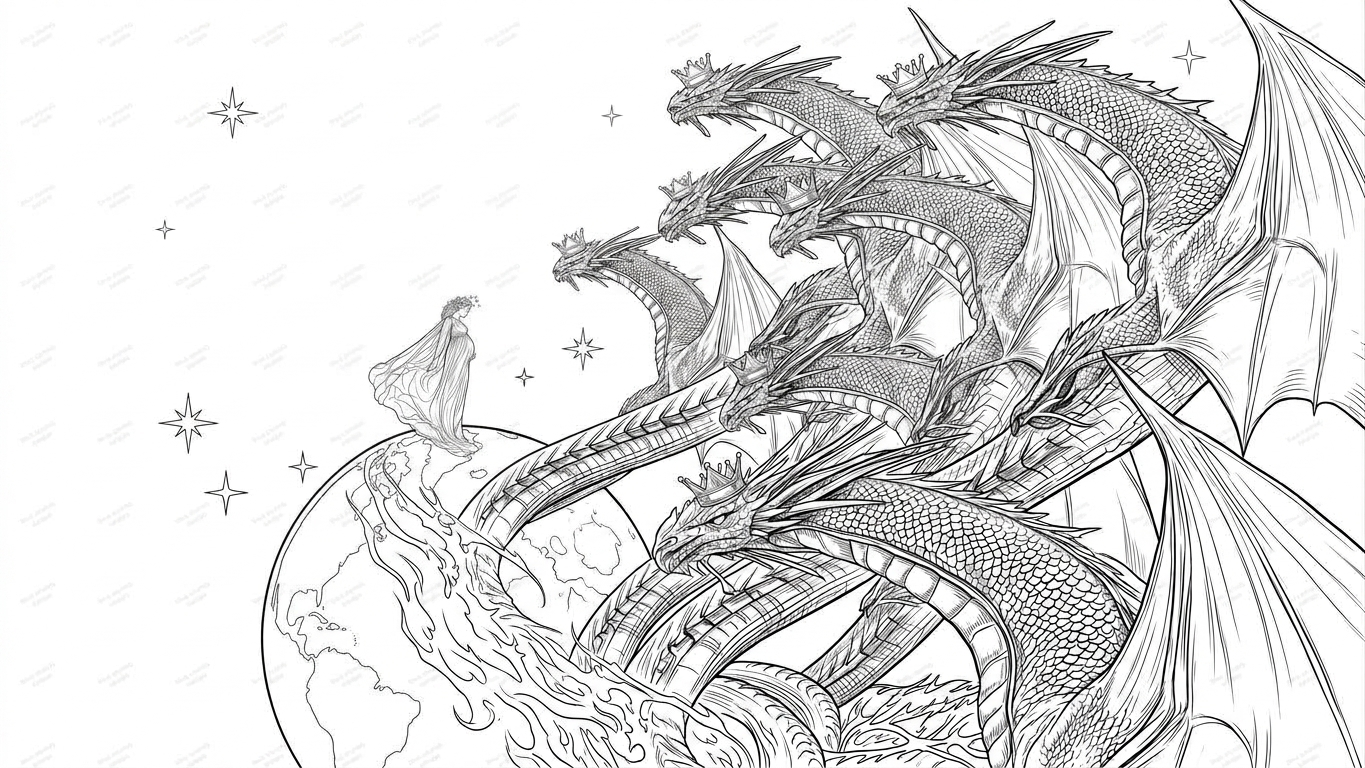
\includegraphics[
    width=1\textwidth,
    trim=0 0 0 0,
    clip]{images/woman_and_dragon2.jpg}
\end{figure}

The woman is clothed with the sun, has the moon beneath her feet, and wears a crown of twelve stars. Readers familiar with Scripture may immediately recall Joseph's dream in Genesis 37:9--11. In that dream, the sun, the moon, and eleven stars represent Jacob, Rachel, and Joseph's eleven brothers. Together with Joseph himself, the twelve stars also evoke the twelve tribes\index{twelve tribes of Israel} of Israel\index{Israel}.

Isaiah, too, repeatedly portrays God's people or Zion as a woman, using this image to describe the relationship between God and His people (Isa. 26:17--18; 49:14--23; 54:1--8; 66:7--9). Isaiah 66:7--9 is particularly significant, describing a woman who gives birth before her labor begins.

Taken together, these Old Testament images suggest that the woman represents Israel and, more broadly, God's covenant people.\footnote{G. K. Beale, \textit{The Book of Revelation: A Commentary on the Greek Text} (Grand Rapids, MI: Eerdmans, 1999), 625.}

Because the woman gives birth to the male child\index{male child}, who is the Messiah\index{Messiah}, Jesus Christ, some interpreters understand her to represent Mary, the mother of Jesus. Yet the imagery of the sun, moon, and twelve stars points more naturally to Israel understood in the broader sense of God's covenant people.

\section{The Male Child: Jesus Christ}\index{male child}

\begin{ScriptureBox2}{What will the male child do, and where is he taken?}

\item[12:5] \textit{She gave birth to a son, a male child, who “will rule all the nations with an iron scepter.” And her child was snatched up to God and to his throne.}

\end{ScriptureBox2}

This verse directly echoes Psalm 2:7--9, which declares, “You are my son; today I have become your father,” and speaks of the king ruling the nations with an iron scepter. The male child\index{male child} is therefore the Messianic King, Jesus Christ.

The vision moves swiftly from the child's birth to the dragon\index{dragon}'s attempt to destroy him, then immediately to the outcome: the child is caught up to God's throne\index{throne of God}. His earthly birth, death, resurrection, and ascension are not narrated in detail. Instead, the vision compresses the great events of redemption into a few striking images.

John is not attempting to recount Jesus' earthly life. His focus is elsewhere: the dragon\index{dragon} cannot destroy the Messiah\index{Messiah} whom God has appointed as King.\footnote{This is an example of a typological or redemptive-historical reading. A typological reading considers how people, events, and institutions in the Old Testament anticipate Christ. A redemptive-historical reading places a passage within the unfolding story of God's plan of salvation, tracing its place in the movement from creation and the Fall to redemption and final fulfillment. The emphasis is on the progression of God's saving work.}


\begin{ScriptureBox2}{Underline the three ways God's people triumph over the accuser in 12:11. How is the woman protected from the dragon, and against whom does the dragon then wage war?}

\item[12:6] The woman fled into the wilderness to a place prepared for her by God, where she might be taken care of for 1,260 days.

\item[12:7] Then war broke out in heaven. Michael and his angels fought against the dragon, and the dragon and his angels fought back.

\item[12:8] But he was not strong enough, and they lost their place in heaven.

\item[12:9] The great dragon was hurled down---that ancient serpent called the devil, or Satan, who leads the whole world astray. He was hurled to the earth, and his angels with him.

\item[12:10] Then I heard a loud voice in heaven say:\\
\hspace*{1em}``Now have come the salvation and the power\\
\hspace*{2em}and the kingdom of our God,\\
\hspace*{2em}and the authority of his Messiah.\\
\hspace*{1em}For the accuser of our brothers and sisters,\\
\hspace*{2em}who accuses them before our God day and night,\\
\hspace*{2em}has been hurled down.

\item[12:11] \hspace*{1em}They triumphed over him\\
\hspace*{2em}by the blood of the Lamb\\
\hspace*{2em}and by the word of their testimony;\\
\hspace*{1em}they did not love their lives so much\\
\hspace*{2em}as to shrink from death.

\item[12:12] \hspace*{1em}Therefore rejoice, you heavens\\
\hspace*{2em}and you who dwell in them!\\
\hspace*{1em}But woe to the earth and the sea,\\
\hspace*{2em}because the devil has gone down to you!\\
\hspace*{1em}He is filled with fury,\\
\hspace*{2em}because he knows that his time is short.''

\item[12:13] When the dragon saw that he had been hurled to the earth, he pursued the woman who had given birth to the male child.

\item[12:14] The woman was given the two wings of a great eagle, so that she might fly to the place prepared for her in the wilderness, where she would be taken care of for a time, times and half a time, out of the serpent's reach.

\item[12:15] Then from his mouth the serpent spewed water like a river, to overtake the woman and sweep her away with the torrent.

\item[12:16] But the earth helped the woman by opening its mouth and swallowing the river that the dragon had spewed out of his mouth.

\item[12:17] Then the dragon was enraged at the woman and went off to wage war against the rest of her offspring---those who keep God's commands and hold fast their testimony about Jesus.

\end{ScriptureBox2}

\begin{figure}[htbp]
    \centering
    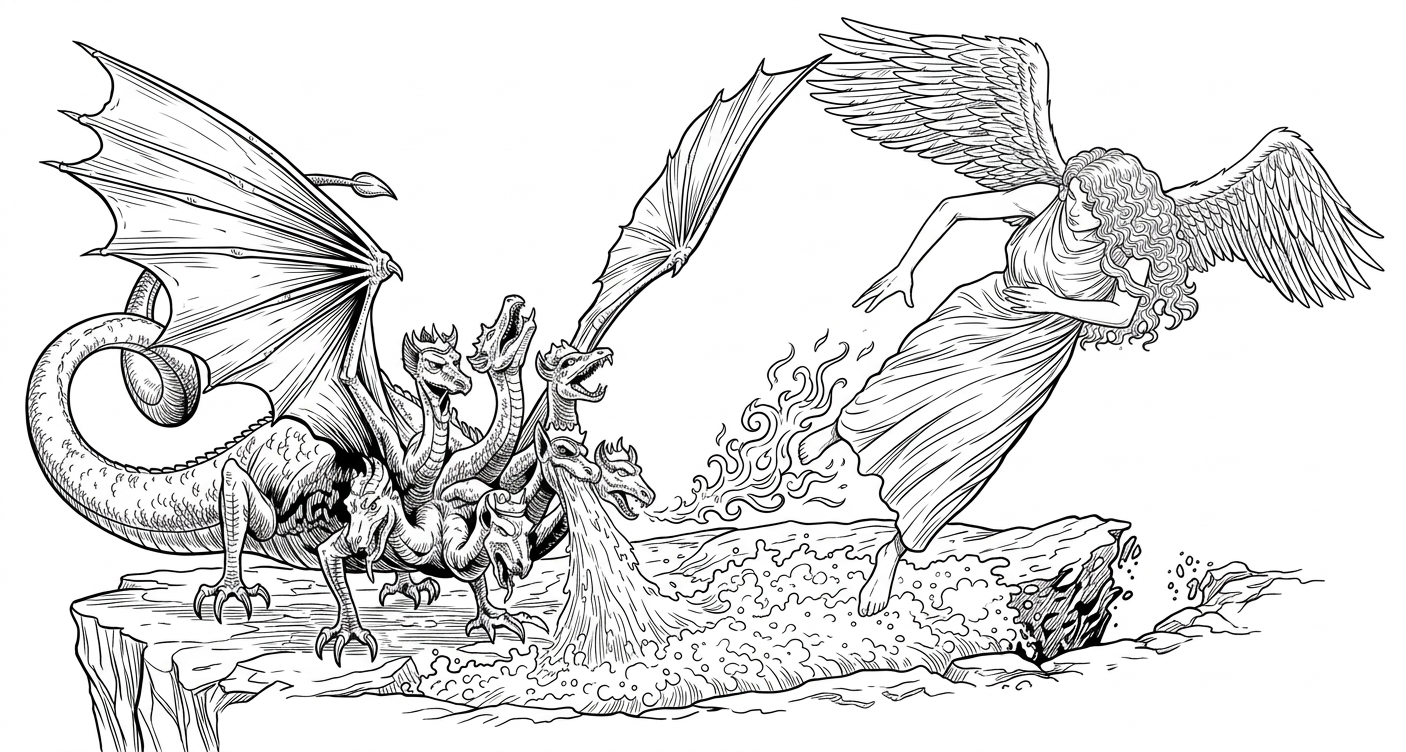
\includegraphics[
    width=1\textwidth,
    trim=0 0 0 0,
    clip]{images/woman_fly_away.jpg}
\end{figure}

The period of 1,260 days\index{1,260 days} is equivalent to three and a half years, using a 360-day year (1,260 divided by 360 equals 3.5). Daniel\index{Daniel} also refers to this period in several visions. Attempts to identify it too rigidly with a specific three-and-a-half-year period in a particular generation, however, can become strained and distract from the vision's central message.


\begin{ReaderQuestion}
The dragon's fury grows fiercer, yet its time is limited by God, and the woman is sustained in the wilderness. When you face a season of trial that seems to intensify rather than ease, how does knowing that God sets its limits and sustains you through it change the way you endure?
\end{ReaderQuestion}



\section{The Beast from the Sea: Imperial Power Opposed to God}\index{beast!from the sea}

\begin{ScriptureBox2}{Circle the animals the beast resembles. Who gives the beast its power, and how long may it exercise its authority?}

\item[13:1] The dragon stood on the shore of the sea. And I saw a beast coming out of the sea. It had ten horns and seven heads, with ten crowns on its horns, and on each head a blasphemous name.
% NIV footnote for 13:1 (omitted; add as \footnote if wanted):
%   ``The dragon'' --- Some later manuscripts And I
% NOTE: some translations number ``The dragon stood on the shore of the sea''
%   as 12:18; the NIV places it at 13:1.

\item[13:2] The beast I saw resembled a leopard, but had feet like those of a bear and a mouth like that of a lion. The dragon gave the beast his power and his throne and great authority.

\item[13:3] One of the heads of the beast seemed to have had a fatal wound, but the fatal wound had been healed. The whole world was filled with wonder and followed the beast.

\item[13:4] People worshiped the dragon because he had given authority to the beast, and they also worshiped the beast and asked, ``Who is like the beast? Who can wage war against it?''

\item[13:5] The beast was given a mouth to utter proud words and blasphemies and to exercise its authority for forty-two months.

\item[13:6] It opened its mouth to blaspheme God, and to slander his name and his dwelling place and those who live in heaven.

\item[13:7] It was given power to wage war against God's holy people and to conquer them. And it was given authority over every tribe, people, language and nation.

\item[13:8] All inhabitants of the earth will worship the beast---all whose names have not been written in the Lamb's book of life, the Lamb who was slain from the creation of the world.
% NIV footnote for 13:8 (omitted; add as \footnote if wanted):
%   ``from the creation of the world'' --- Or written from the creation of
%   the world in the book of life belonging to the Lamb who was slain

\item[13:9] Whoever has ears, let them hear.

\item[13:10] \hspace*{1em}``If anyone is to go into captivity,\\
\hspace*{2em}into captivity they will go.\\
\hspace*{1em}If anyone is to be killed with the sword,\\
\hspace*{2em}with the sword they will be killed.''\\
This calls for patient endurance and faithfulness on the part of God's people.
% NIV footnotes for 13:10 (omitted; add as \footnote if wanted):
%   ``is to be killed'' --- Some manuscripts anyone kills
%   ``they will be killed'' --- Jer. 15:2
% CHECK NIV: all footnote wording in this passage quoted from memory;
%   verify against Bible Gateway.

\end{ScriptureBox2}

The beast\index{beast} represents earthly imperial power opposed to God. We see the foundation for this interpretation in Daniel\index{Daniel}. Daniel 7 describes four beasts rising from the sea and explains that they represent four kings who will arise on the earth. Daniel 8 then presents the vision of a ram and a goat, foretelling the rise of Medo-Persia and Greece, the emergence of a Greek king, and the subsequent division of the Greek empire.\footnote{The king is commonly identified as Alexander the Great (Dan. 8:21), who conquered Persia in the fourth century BC, roughly two centuries after the time traditionally associated with Daniel.}

These visions establish an important pattern: beasts represent earthly rulers and imperial powers.

In Revelation, after the dragon\index{dragon} is cast down, it takes its stand on the shore of the sea. What does it do next? It brings into view the beast from the sea\index{beast!from the sea} and the beast from the earth\index{beast!from the earth}. What, then, does the sea beast represent? Its features point directly back to Daniel 7.

In Revelation, the sea symbolizes the peoples and nations of the world. Revelation 17:15 explicitly interprets the waters as peoples, multitudes, nations, and languages. The beast rising from the sea therefore represents earthly power emerging from among the nations and standing in opposition to God and His people.

Table \ref{tab:rev13-daniel7} compares the vision in Revelation 13 with its Old Testament background in Daniel 7.

{
\renewcommand{\arraystretch}{1}
\small
\begin{longtable}{>{\raggedright\arraybackslash}p{3cm}
                  >{\raggedright\arraybackslash}p{3.5cm}
                  >{\raggedright\arraybackslash}p{2.7cm}}
\caption{The beast of Revelation 13 and the beasts of Daniel 7}
\label{tab:rev13-daniel7} \\
\hline
Revelation 13 &
Daniel 7 &
Significance \\
\hline
\endfirsthead

\multicolumn{3}{l}{\small\itshape Table~\thetable\ (continued)} \\
\hline
Revelation 13 &
Daniel 7 &
Significance \\
\hline
\endhead

\hline
\endfoot

\hline
\endlastfoot

1: The beast rises from the sea &
2--3: Four beasts rise from the sea &
Empires among the nations \\

2: The beast has a lion's mouth &
4: The first beast resembles a lion &
Lion imagery \\

2: The beast has feet like a bear's &
5: The second beast resembles a bear &
Bear imagery \\

2: The beast resembles a leopard &
6: The third beast resembles a leopard &
Leopard imagery \\

1: The beast possesses terrifying power &
7: The fourth beast is exceedingly terrifying &
Power surpassing that of earlier empires \\

1: The beast has ten horns &
7: The fourth beast has ten horns &
Imperial power \\

6: The beast speaks blasphemies &
8: The little horn speaks boastfully &
Usurping God's authority \\

7: The beast wages war against the saints &
21: The little horn wages war against the holy people &
Persecution of God's people \\

7: The beast overcomes the saints &
21: The little horn overpowers them &
A temporary victory \\

The Lamb ultimately judges the beast &
22: The Ancient of Days takes His place in judgment &
Final judgment \\

5: Forty-two months &
25: A time, times, and half a time &
A limited period of persecution \\

7: The beast is permitted to wage war against the saints &
25: The holy people are handed over to the beast &
God permits but limits its power \\

The beast faces God's judgment &
26--27: The beast's dominion is finally taken away &
The beast's ultimate defeat \\

\end{longtable}
}

\begin{ReaderQuestion}
In Table~\ref{tab:rev13-daniel7}, the beast of Revelation 13 combines features of all four beasts in Daniel 7: the lion, the bear, the leopard, and the ten horns. It even ``overcomes the saints,'' yet the table ends with its dominion taken away. What powers in today's world seem impressive or frightening to you, and how does this table help you see them in light of God's final judgment?
\end{ReaderQuestion}

One of the most striking features of this vision is that the dragon\index{dragon} gives its authority to the sea beast. One of the beast's heads appears to have suffered a fatal wound, yet the wound is healed, and the whole world marvels and follows the beast. Here we see a counterfeit of Christ's death and resurrection.

The true Christ suffered death, rose again, and was exalted in glory. The beast, by contrast, appears to have died but recovers, and then receives the worship\index{worship} of the world. It imitates the pattern of Christ's victory, offering a deceptive spectacle in place of the true work of redemption.

\begin{figure}[htbp]
    \centering
    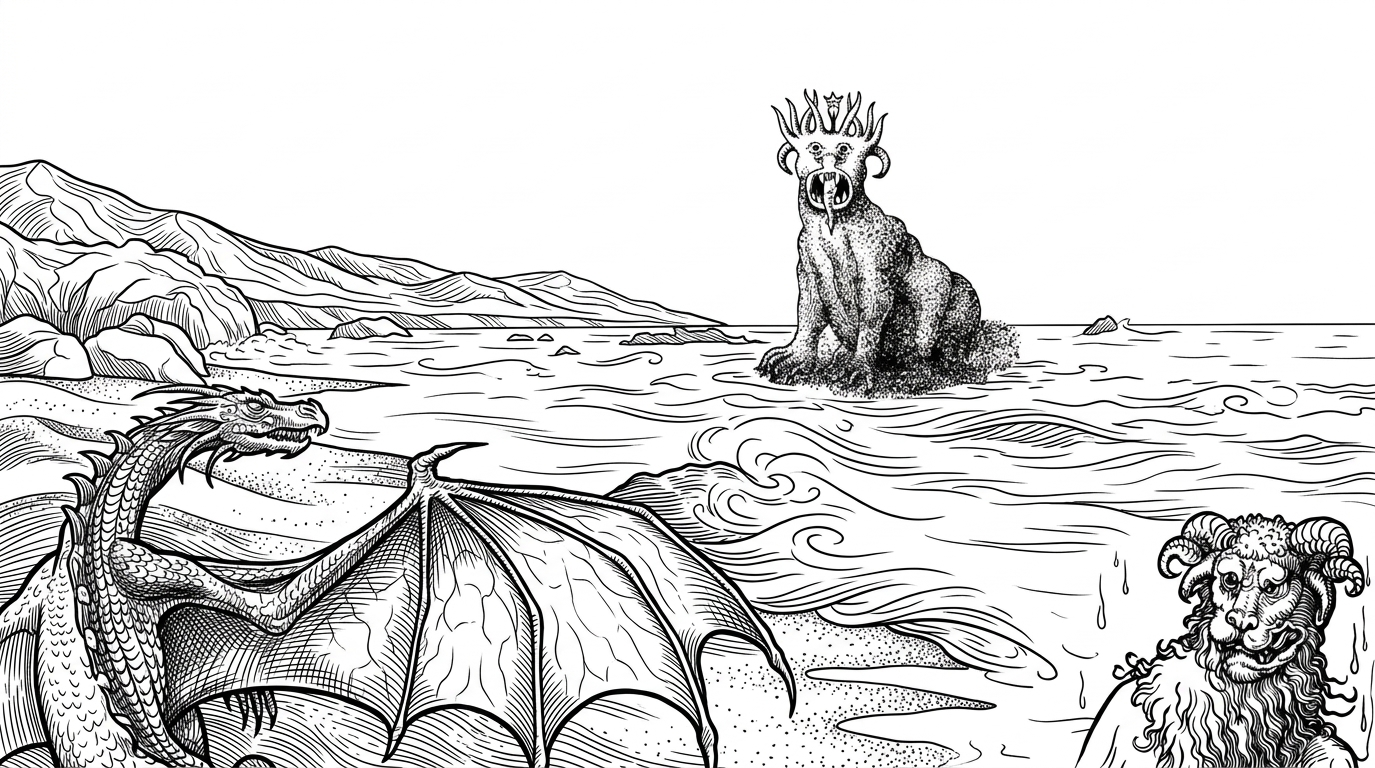
\includegraphics[
    width=1\textwidth,
    trim=0 0 0 0,
    clip]{images/dragon_and_breast.jpg}
\end{figure}

\section{The Beast from the Earth: The False Prophet}\index{beast!from the earth}\index{false prophet}

\begin{ScriptureBox2}{What does the second beast look like, and how does it speak? Underline everything it makes the inhabitants of the earth do.}

\item[13:11] Then I saw a second beast, coming out of the earth. It had two horns like a lamb, but it spoke like a dragon.

\item[13:12] It exercised all the authority of the first beast on its behalf, and made the earth and its inhabitants worship the first beast, whose fatal wound had been healed.

\item[13:13] And it performed great signs, even causing fire to come down from heaven to the earth in full view of the people.

\item[13:14] Because of the signs it was given power to perform on behalf of the first beast, it deceived the inhabitants of the earth. It ordered them to set up an image in honor of the beast who was wounded by the sword and yet lived.

\item[13:15] The second beast was given power to give breath to the image of the first beast, so that the image could speak and cause all who refused to worship the image to be killed.

\end{ScriptureBox2}

Now we turn to the beast from the earth\index{beast!from the earth}. It has two horns like a lamb, yet it speaks like a dragon\index{dragon}. Its appearance suggests innocence and even a resemblance to the Lamb, but its voice betrays its true allegiance. This is a deceptive religious power. Later, Revelation 16:13, 19:20, and 20:10 identify it as the false prophet\index{false prophet}.

\begin{ReaderQuestion}
The beast from the earth looks like a lamb but speaks like a dragon. How does this image help us discern teachings that appear godly on the surface but are actually deceptive?
\end{ReaderQuestion}

The beast from the earth\index{beast!from the earth} is therefore not simply another political empire. It operates under the authority of the first beast, performing signs, deceiving people, promoting the worship of the beast\index{beast}, and leading the inhabitants of the earth to accept its mark.

Together, the dragon\index{dragon}, the beast from the sea\index{beast!from the sea}, and the beast from the earth\index{beast!from the earth} form a counterfeit trinity. The dragon imitates God, the sea beast imitates the Lamb, and the false prophet\index{false prophet} imitates the work of the Holy Spirit\index{Holy Spirit}. Their apparent unity is a dark parody of the true God: a counterfeit kingdom that seeks to claim the worship, allegiance, and trust that belong to God alone.

\begin{ReaderQuestion}
How do the dragon, the beast from the sea, and the beast from the earth work together to imitate God's authority and oppose Him? What does this teach us about spiritual warfare?
\end{ReaderQuestion}

\section{The Number of Man: 666}\index{666}

\begin{ScriptureBox2}{Who is forced to receive the mark, and where is it placed? What can people not do without it?}

\item[13:16] It also forced all people, great and small, rich and poor, free and slave, to receive a mark on their right hands or on their foreheads,

\item[13:17] so that they could not buy or sell unless they had the mark, which is the name of the beast or the number of its name.

\item[13:18] This calls for wisdom. Let the person who has insight calculate the number of the beast, for it is the number of a man. That number is 666.
% NIV footnote for 13:18 (omitted; add as \footnote if wanted):
%   ``the number of a man'' --- Or is humanity's number
% CHECK NIV: footnote wording quoted from memory; verify against Bible Gateway.

\end{ScriptureBox2}

Those who receive the beast\index{beast}'s mark are permitted to buy and sell. Those who refuse it, by contrast, face exclusion from ordinary economic life. God's servants who will not accept the mark may find themselves unable to participate in the marketplace and forced to rely on barter or other means of survival. Their refusal to worship the beast comes at a considerable cost.

Yet they remain faithful to the truth: only the Lamb who was slain\index{Lamb, the!slain} is worthy of worship. Through the blood of the Lamb\index{Lamb, the!blood of} and the faithful testimony they maintain, His people overcome\index{overcomers} even amid the beast's persecution\index{persecution}.

Why is the number 666\index{666} rather than 777? It is unwise to treat 666 simply as a secret code that can be used to identify some particular person, object, or technology. In Scripture, the number seven is often associated with completeness or fullness. The triple six, by contrast, can be understood as a picture of radical incompleteness: a repeated falling short of the fullness represented by seven. The contrast is striking. God's perfection stands in opposition to the beast's arrogant self-exaltation, which can never attain the fullness that belongs to God.

Some have associated the beast's mark with modern technology, barcodes, microchips, identity cards, or cashless payment systems. Such associations may arise naturally when modern readers reflect on the text, but they should not be treated as direct predictions of particular future technologies. The passage's central concern is allegiance and worship: whom people worship, to whom they give their loyalty, and how that loyalty can expose them to social and economic persecution\index{persecution}.

\begin{ReaderQuestion}
How does the mark of the beast contrast with the faithfulness of God's people? When faith conflicts with economic interests or social pressure, how can we remain steadfast?
\end{ReaderQuestion}

\section{The Lamb and His People}\index{Lamb, the}

The vision of the dragon\index{dragon}, the sea beast, and the earth beast presents a disturbing counterfeit of the divine order. Yet chapter 14 redirects our gaze to the Lamb.

John sees the Lamb standing on Mount Zion, accompanied by 144,000\index{144,000} people. The names of the Lamb and His Father are written on their foreheads, marking them as belonging to God rather than to the beast\index{beast}. They follow the Lamb wherever He goes, remaining faithful to God's commandments and to their testimony about Jesus even through times of tribulation.

The counterfeit trinity of chapter 13 stands in sharp contrast to the Lamb and His people in chapter 14. The beast demands worship, but the Lamb's people worship Him. The world may use power, fear, and material advantage to pressure people into compromise, but God knows those who belong to Him. The mark of the beast\index{beast!mark of} may appear to determine who can participate in earthly society; the name of the Lamb reveals who truly belongs to the kingdom that will endure.

Then three angels announce the coming judgment\index{judgment}. The first proclaims the eternal gospel\index{eternal gospel}, calling all nations to fear God and give Him glory. The second announces the fall of Babylon\index{Babylon}. The third warns that those who worship the beast will face God's judgment. Finally, two harvest\index{harvest} visions bring us to the end of the age: the grain is ripe, the grapes are fully mature, and God's judgment will surely come.

Amid these solemn warnings, however, God gives His people a precious word of comfort:

“Blessed are the dead who die in the Lord.”

Though they have labored on earth and some have even laid down their lives for Christ, their labor has not been in vain. They will rest from their toil, and their deeds will follow them. The world may forget their faithfulness, but the Lord does not. The Lamb who calls them to endure is the same Lamb who will receive them into His presence.

\begin{ScriptureBox2}{What is written on the foreheads of the 144,000? Underline every phrase that describes them in 14:4--5.}

\item[14:1] Then I looked, and there before me was the Lamb, standing on Mount Zion, and with him 144,000 who had his name and his Father's name written on their foreheads.

\item[14:2] And I heard a sound from heaven like the roar of rushing waters and like a loud peal of thunder. The sound I heard was like that of harpists playing their harps.

\item[14:3] And they sang a new song before the throne and before the four living creatures and the elders. No one could learn the song except the 144,000 who had been redeemed from the earth.

\item[14:4] These are those who did not defile themselves with women, for they remained virgins. They follow the Lamb wherever he goes. They were purchased from among mankind and offered as firstfruits to God and the Lamb.

\item[14:5] No lie was found in their mouths; they are blameless.

\end{ScriptureBox2}

%\begin{figure}[htbp]
%    \centering
%    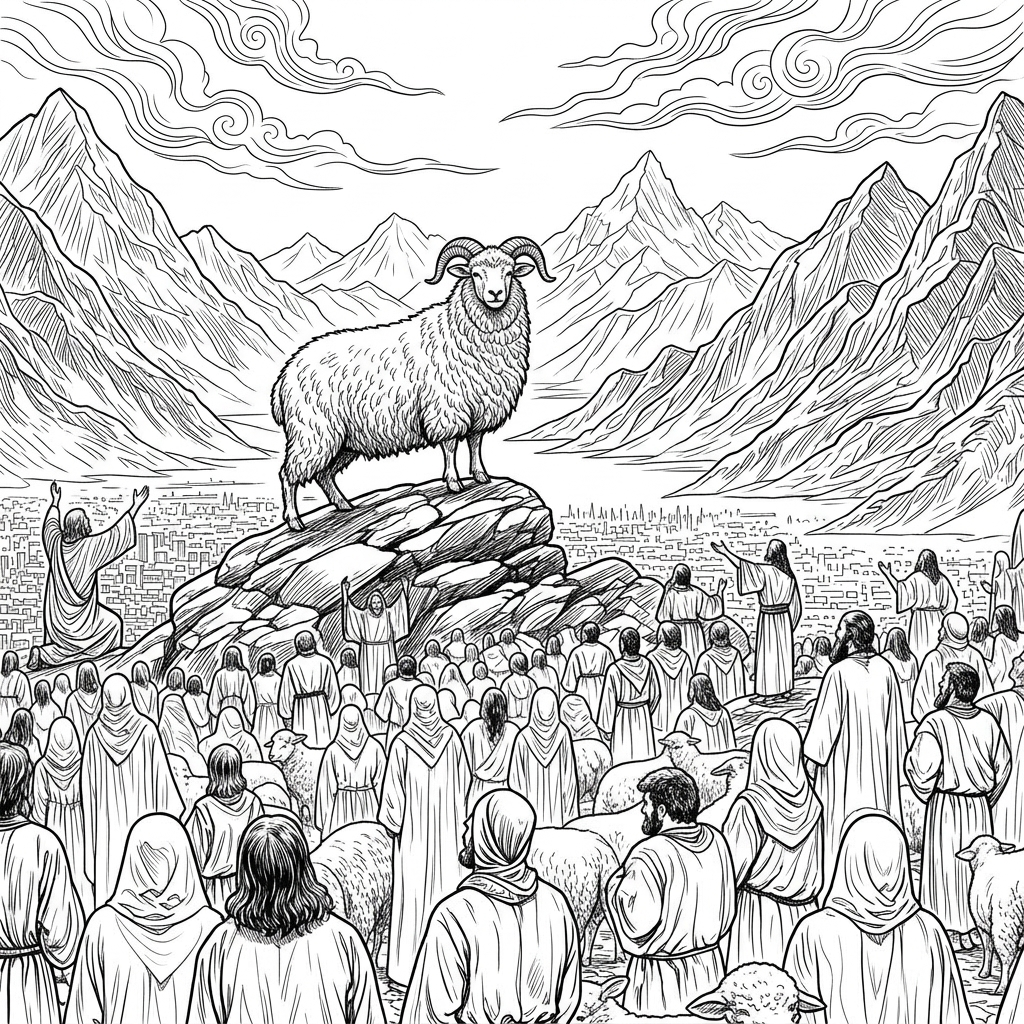
\includegraphics[
%    width=1\textwidth,
%    trim=0 0 0 0,
%    clip]{images/lamb_14400.jpg}
%\end{figure}

These people are described as having been “purchased from among mankind and offered as firstfruits to God and the Lamb.” They are redeemed by Jesus and belong to Him. The declaration that no lie is found in their mouths and that they are blameless does not mean that they have achieved sinless perfection through their own efforts. Rather, they stand before the Lamb as those who belong to Him, cleansed and made acceptable through His redemptive work.

They are also described as those who “did not defile themselves with women, for they remained virgins.” Some interpret this description literally, understanding them to be unmarried men who have abstained from sexual relations. Yet the Old Testament frequently uses the imagery of marriage and sexual unfaithfulness to portray faithfulness or unfaithfulness to God. In this context, the language also conveys the idea of undivided loyalty to the Lamb. Wherever He goes, they follow.

\begin{ReaderQuestion}
What does it mean to you personally to follow the Lamb wherever He goes (Rev. 14:4)?
\end{ReaderQuestion}

Their song is unlike any other. It is a song born of a journey through redemption, a song that can be learned only by those who have walked the path themselves and remained steadfast through trial. Its melody rises from lives purchased by the Lamb and kept faithful to Him. No one else can learn this new song, because its praise springs from an experience of grace and perseverance known only to those who have followed the Lamb through suffering.

\section{The Angels Proclaim the Eternal Gospel}\index{eternal gospel}

\begin{ScriptureBox2}{Underline what each of the three angels proclaims. Who are called blessed in 14:13, and why?}

\item[14:6] Then I saw another angel flying in midair, and he had the eternal gospel to proclaim to those who live on the earth---to every nation, tribe, language and people.

\item[14:7] He said in a loud voice, ``Fear God and give him glory, because the hour of his judgment has come. Worship him who made the heavens, the earth, the sea and the springs of water.''

\item[14:8] A second angel followed and said, ``\,`Fallen! Fallen is Babylon the Great,' which made all the nations drink the maddening wine of her adulteries.''
% NIV footnote for 14:8 (omitted; add as \footnote if wanted):
%   ``Fallen is Babylon the Great'' --- Isaiah 21:9
% CHECK NIV: footnote reference quoted from memory; verify against Bible Gateway.

\item[14:9] A third angel followed them and said in a loud voice: ``If anyone worships the beast and its image and receives its mark on their forehead or on their hand,

\item[14:10] they, too, will drink the wine of God's fury, which has been poured full strength into the cup of his wrath. They will be tormented with burning sulfur in the presence of the holy angels and of the Lamb.

\item[14:11] And the smoke of their torment will rise for ever and ever. There will be no rest day or night for those who worship the beast and its image, or for anyone who receives the mark of its name.''

\item[14:12] This calls for patient endurance on the part of the people of God who keep his commands and remain faithful to Jesus.

\item[14:13] Then I heard a voice from heaven say, ``Write this: Blessed are the dead who die in the Lord from now on.''\\
``Yes,'' says the Spirit, ``they will rest from their labor, for their deeds will follow them.''

\end{ScriptureBox2}

\begin{figure}[h]
    \centering
    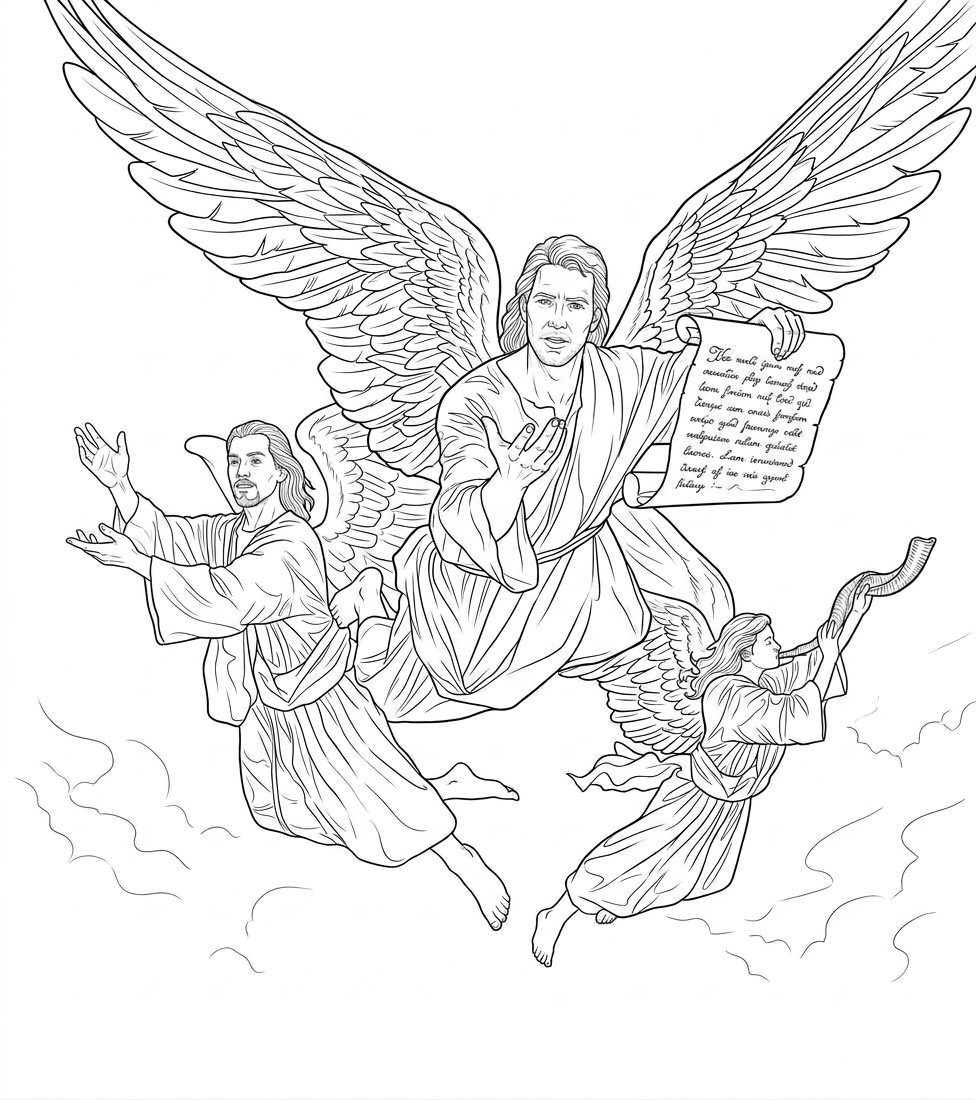
\includegraphics[
    width=0.8\textwidth,
    trim=0 0 0 0,
    clip]{images/eternal_gospel.jpg}
\end{figure}

Even at this late hour, the gospel is still proclaimed to the inhabitants of the earth. What does this eternal gospel\index{eternal gospel} declare? It calls people to fear God, give Him glory, and worship the One who made the heavens, the earth, the sea, and the springs of water.

Our very existence is a gift of the Creator\index{Creator}. As creatures who have received the grace of life, we are called to respond by worshiping God and giving Him the glory that belongs to Him. The eternal gospel\index{eternal gospel} therefore summons all people to recognize their Creator and turn to Him in reverence and worship.

\begin{ReaderQuestion}
What does the first angel's proclamation of the “eternal gospel” include (Rev. 14:6--7)? Why are fearing God, giving Him glory, and worshiping the Creator integral to the message of the gospel?
\end{ReaderQuestion}

The next two angels announce God's righteous judgment. Those who rebel against their Creator\index{Creator} reject not only the grace of being created but also the redeeming blood of Jesus Christ. They give their allegiance to the beast\index{beast}, receive its mark, and persecute\index{persecution} the saints. God's judgment upon those who persist in such rebellion is therefore not arbitrary. It is the just response of the holy God to the rejection of His rule and the oppression of His people.

Yet for those who persevere in faith, and for those who die in the Lord, there is a blessed promise. They truly rest from their toil, and the fruit of their labor for Christ follows them. What a profound comfort this is to those who have spent their lives serving the Lord, often without recognition, and sometimes at great personal cost. Their work may appear small in the eyes of the world, but it is not forgotten in heaven.

\section{The Two Visions of the Harvest}\index{harvest}

\begin{ScriptureBox2}{Compare the two harvests. Who swings the first sickle, what is gathered in the second, and where is it thrown?}

\item[14:14] I looked, and there before me was a white cloud, and seated on the cloud was one like a son of man with a crown of gold on his head and a sharp sickle in his hand.
% NIV footnote for 14:14 (omitted; add as \footnote if wanted):
%   ``son of man'' --- See Daniel 7:13.

\item[14:15] Then another angel came out of the temple and called in a loud voice to him who was sitting on the cloud, ``Take your sickle and reap, because the time to reap has come, for the harvest of the earth is ripe.''

\item[14:16] So he who was seated on the cloud swung his sickle over the earth, and the earth was harvested.

\item[14:17] Another angel came out of the temple in heaven, and he too had a sharp sickle.

\item[14:18] Still another angel, who had charge of the fire, came from the altar and called in a loud voice to him who had the sharp sickle, ``Take your sharp sickle and gather the clusters of grapes from the earth's vine, because its grapes are ripe.''

\item[14:19] The angel swung his sickle on the earth, gathered its grapes and threw them into the great winepress of God's wrath.

\item[14:20] They were trampled in the winepress outside the city, and blood flowed out of the press, rising as high as the horses' bridles for a distance of 1,600 stadia.
% NIV footnote for 14:20 (omitted; add as \footnote if wanted):
%   ``1,600 stadia'' --- That is, about 180 miles or about 300 kilometers
% CHECK NIV: footnote wording quoted from memory; verify against Bible Gateway.

\end{ScriptureBox2}

As discussed in earlier chapters, the figure described here as “one like a son of man\index{Son of Man}” is Jesus Christ. The harvest\index{harvest} is ripe, and He holds a sharp sickle in His hand, ready to reap the earth.

In John 4:35, Jesus speaks of the harvest\index{harvest} in words familiar to those who work the land. He tells His disciples to lift their eyes and look at the fields, for they are ripe for harvest. Imagine a field of golden grain, its heavy heads bending in the light, while workers move through it with sharp sickles. What a joyful sight it is when the harvest has come!

Yet harvest\index{harvest} is also an image of judgment. The grain and the weeds are separated: the grain is gathered into the barn, while the weeds are burned. In Matthew 13:24--30, Jesus uses a parable drawn from ordinary agricultural life to teach this truth. The farmer does not attempt to separate the wheat from the weeds while the plants are still young. Both are allowed to grow together until the harvest, when their true nature becomes clear and they can be separated.\footnote{Matthew 13:24--30 recounts Jesus' parable of the wheat and the weeds. An enemy sows weeds among the wheat while the household sleeps. When the plants grow, the servants ask whether they should pull out the weeds. The owner refuses, lest they uproot the wheat as well. Both are to grow together until the harvest, when the weeds will be gathered and burned and the wheat brought into the barn. Insert the licensed NIV text here if the full passage is to be quoted.}

The connection between harvest\index{harvest} and judgment is made explicit in Joel 3:13, which calls for the sickle to be put in because the harvest is ripe, and for the winepress\index{winepress} to be trodden because the winepress is full and the vats overflow with the wickedness of the nations.

In Revelation, an angel swings his sickle over the earth and gathers the grapes, throwing them into the great winepress\index{winepress} of God's wrath\index{wrath of God}. The time of judgment has arrived. The image is terrible in its force: the wickedness of the earth has ripened, and the judgment of God can no longer be deferred.

As grapes are crushed in the winepress until the vats overflow, so the vision portrays the overwhelming severity of divine judgment. The blood rises as high as the horses' bridles and extends for a distance of 1,600 stadia, a scene of judgment rendered in stark and unforgettable imagery.

\begin{ReaderQuestion}
Revelation 14 shows two harvests: the grain gathered by the Son of Man and the grapes thrown into the winepress of God's wrath. Since the final harvest has not yet come, how should God's patience today shape the way you respond to Him, and the way you speak to others about Him?
\end{ReaderQuestion}

\begin{figure}[htbp]
    \centering
    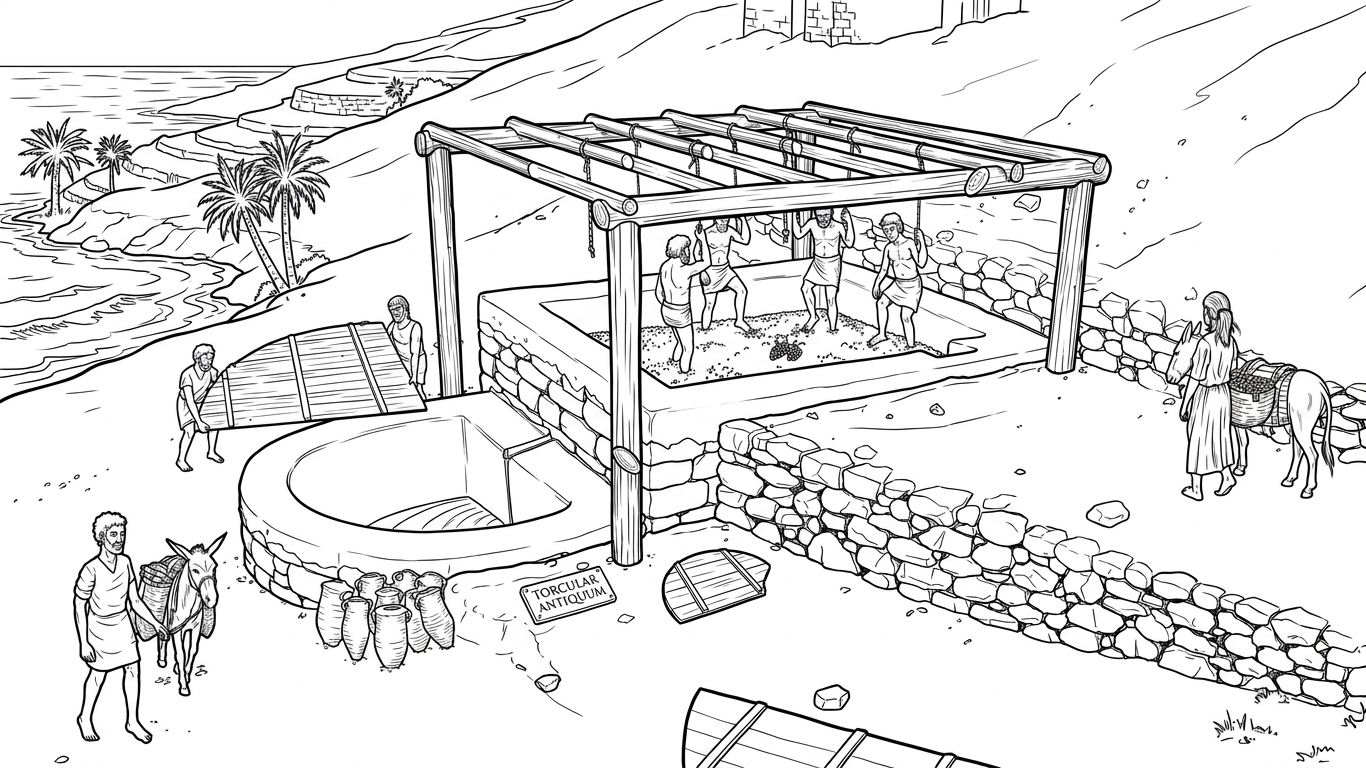
\includegraphics[
    width=1\textwidth,
    trim=0 0 0 0,
    clip]{images/wine_pressing.jpg}
\end{figure}

\chapter{The Fullness of God's Wrath and His Righteous Judgment (15:1--16:21)}\index{judgment}\index{wrath of God}

If the seven seals\index{seals, seven} and seven trumpets\index{trumpets, seven} have gradually unveiled the judgments\index{judgment} of God, then in Revelation 15 and 16 those judgments enter their final stage. John sees seven angels entrusted with the seven last plagues\index{plagues}. They carry seven golden bowls filled with the wrath\index{wrath of God} of God and pour them out upon the earth.

Yet before the terrible judgments unfold, John is given a vision of victory. Those who have overcome\index{overcomers} the beast\index{beast}, its image, and the number of its name stand beside a sea of glass\index{sea of glass}, holding harps given them by God. They sing the song of Moses\index{Song of Moses} and the song of the Lamb\index{Song of the Lamb}.

This sequence is profoundly significant. Before the judgments descend, John shows us the victorious people of God. Those who belong to the Lamb\index{Lamb, the} do not stand condemned beneath God's wrath; they stand secure in His keeping. They have passed through tribulation without bowing before the beast, and at last they stand before God, rejoicing in His presence and worshiping\index{worship} Him. The final vision of judgment begins, therefore, not with the triumph of evil, but with the song of a redeemed\index{redemption} people whose victory rests in God.

\section{Singing the Song of the Lamb}\index{Song of the Lamb}

\begin{ScriptureBox2}{Circle what those beside the sea of glass are holding and whose song they sing. Underline the words that describe God's deeds and ways in 15:3.}

\item[15:1] I saw in heaven another great and marvelous sign: seven angels with the seven last plagues---last, because with them God's wrath is completed.

\item[15:2] And I saw what looked like a sea of glass glowing with fire and, standing beside the sea, those who had been victorious over the beast and its image and over the number of its name. They held harps given them by God

\item[15:3] and sang the song of God's servant Moses and of the Lamb:\\
\hspace*{1em}``Great and marvelous are your deeds,\\
\hspace*{2em}Lord God Almighty.\\
\hspace*{1em}Just and true are your ways,\\
\hspace*{2em}King of the nations.
% NIV footnote for 15:3 (omitted; add as \footnote if wanted):
%   ``King of the nations'' --- Some manuscripts ages

\item[15:4] \hspace*{1em}Who will not fear you, Lord,\\
\hspace*{2em}and bring glory to your name?\\
\hspace*{1em}For you alone are holy.\\
\hspace*{1em}All nations will come\\
\hspace*{2em}and worship before you,\\
\hspace*{1em}for your righteous acts have been revealed.''
% NIV footnote for 15:4 (omitted; add as \footnote if wanted):
%   end of song --- Phrases in this song are drawn from Psalm 111:2,3;
%   Deut. 32:4; Jer. 10:7; Psalms 86:9; 98:2.
% CHECK NIV: footnote wording quoted from memory; verify against Bible Gateway.

\item[15:5] After this I looked, and I saw in heaven the temple---that is, the tabernacle of the covenant law---and it was opened.

\item[15:6] Out of the temple came the seven angels with the seven plagues. They were dressed in clean, shining linen and wore golden sashes around their chests.

\item[15:7] Then one of the four living creatures gave to the seven angels seven golden bowls filled with the wrath of God, who lives for ever and ever.

\item[15:8] And the temple was filled with smoke from the glory of God and from his power, and no one could enter the temple until the seven plagues of the seven angels were completed.

\end{ScriptureBox2}

Revelation 15 echoes Exodus 15 in striking ways. As shown in Table \ref{tab:rev_exdus_15}, when Moses\index{Moses} and the Israelites passed through the Red Sea, Pharaoh and his army were swallowed by its waters. Having witnessed God's deliverance, Moses and the people broke into a song of triumph. In Revelation 15, the song rises once more, but now it celebrates the Lamb's final victory: He has redeemed His people and overcome\index{overcomers} every power that sets itself against God.

This is not a song that celebrates human courage or achievement. It proclaims the greatness of God's works: they are “great and marvelous”; His ways are “just and true.” When suffering narrows our vision until we can see little beyond our own circumstances, this song lifts our eyes again to the Lord. The final word belongs not to the beast\index{beast}, nor to the powers that persecute\index{persecution} God's people, but to the God whose works are wonderful and whose ways are righteous.

\begin{ReaderQuestion}
In Revelation 15:3--4, the song does not celebrate human courage but proclaims that God's works are “great and marvelous” and His ways “just and true.” When suffering draws our attention toward our own circumstances, how does this song turn our eyes back to God?
\end{ReaderQuestion}

{
\small
\renewcommand{\arraystretch}{1}
\label{tab:rev_exdus_15}
\noindent
\begin{tabular}{@{}L{2.8cm} L{2.8cm} L{3.2cm}@{}}
\hline
Revelation 15 & Exodus 15 & Theme \\
\hline
Verse 1: The seven plagues & The ten plagues of Egypt & God judges His enemies \\
Verse 2: Standing beside the sea of glass & Crossing the Red Sea & God delivers His people \\
Verse 2: The beast & Pharaoh and the Egyptian army & God contends with His enemies \\
Verse 3: The song of Moses and the Lamb & The song of Moses & A song of victory after redemption \\
Verse 5: The sanctuary containing the covenant tablets & The tabernacle and sanctuary & The presence of God \\
Verse 8: Smoke filling the sanctuary & The glory of God & God's presence and judgment \\
\hline
\end{tabular}
\par
}

The angels receive their bowls and prepare to pour them out upon the earth. Below, the world is about to be struck by judgment; above, the heavenly sanctuary stands filled with the glory\index{glory} of God. No one can enter it until the seven plagues\index{plagues} entrusted to the angels have run their course. The judgment proceeding from heaven is neither accidental nor beyond God's authority. It unfolds under the sovereignty of the One whose holiness fills His sanctuary.

\section{The First Five Bowls}

\begin{figure}[htbp]
    \centering
    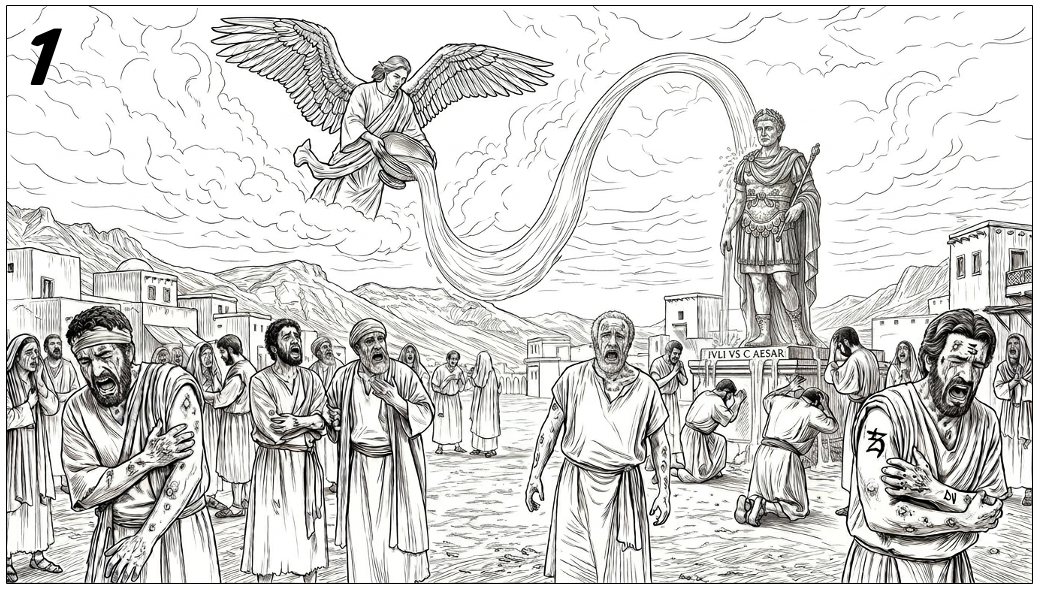
\includegraphics[
    width=1\textwidth,
    trim=0 0 0 0,
    clip]{images/bowl_1.png}
\end{figure}

\begin{figure}[htbp]
    \centering
    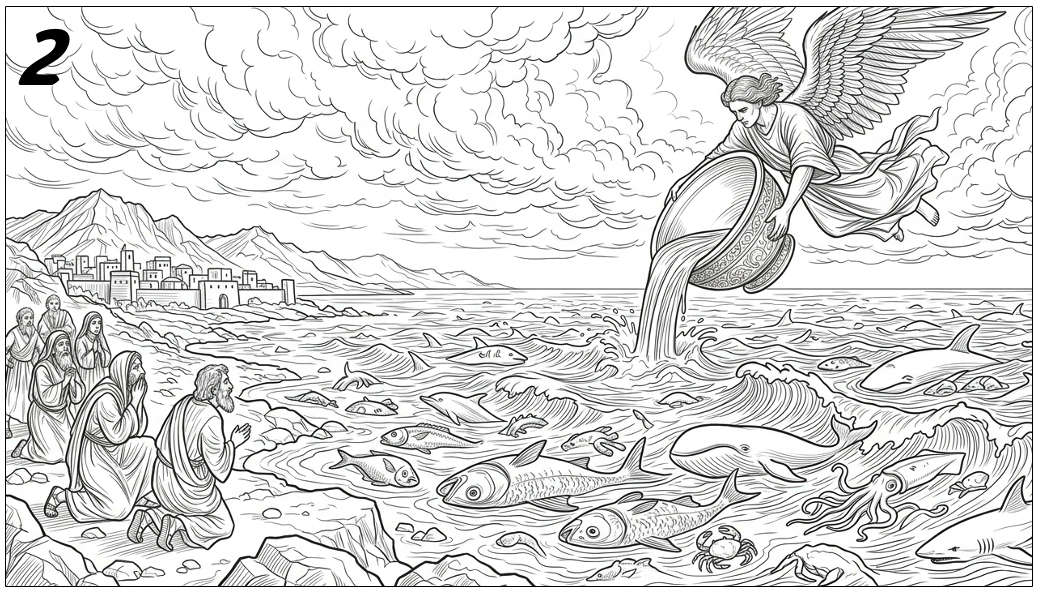
\includegraphics[
    width=1\textwidth,
    trim=0 0 0 0,
    clip]{images/bowl_2.png}
\end{figure}

\begin{ScriptureBox2}{Where is each of the first five bowls poured out? Underline how the people respond in 16:9 and 16:11.}

\item[16:1] Then I heard a loud voice from the temple saying to the seven angels, ``Go, pour out the seven bowls of God's wrath on the earth.''

\item[16:2] The first angel went and poured out his bowl on the land, and ugly, festering sores broke out on the people who had the mark of the beast and worshiped its image.

\item[16:3] The second angel poured out his bowl on the sea, and it turned into blood like that of a dead person, and every living thing in the sea died.

\item[16:4] The third angel poured out his bowl on the rivers and springs of water, and they became blood.

\item[16:5] Then I heard the angel in charge of the waters say:\\
\hspace*{1em}``You are just in these judgments, O Holy One,\\
\hspace*{2em}you who are and who were;

\item[16:6] \hspace*{1em}for they have shed the blood of your holy people and your prophets,\\
\hspace*{2em}and you have given them blood to drink as they deserve.''

\item[16:7] And I heard the altar respond:\\
\hspace*{1em}``Yes, Lord God Almighty,\\
\hspace*{2em}true and just are your judgments.''

\item[16:8] The fourth angel poured out his bowl on the sun, and the sun was allowed to scorch people with fire.

\item[16:9] They were seared by the intense heat and they cursed the name of God, who had control over these plagues, but they refused to repent and glorify him.

\item[16:10] The fifth angel poured out his bowl on the throne of the beast, and its kingdom was plunged into darkness. People gnawed their tongues in agony

\item[16:11] and cursed the God of heaven because of their pains and their sores, but they refused to repent of what they had done.

\end{ScriptureBox2}

\begin{figure}[htbp]
    \centering
    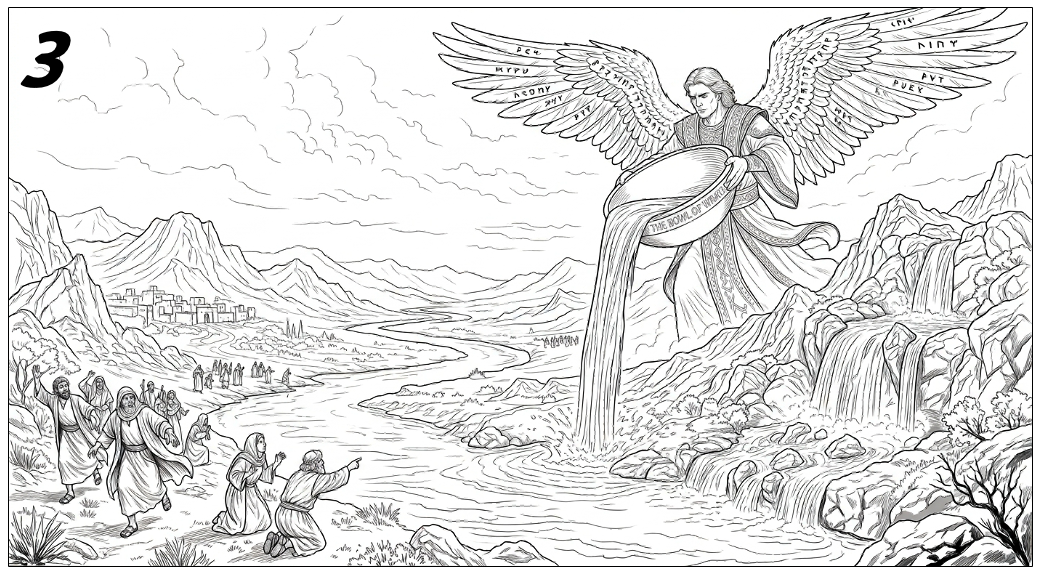
\includegraphics[
    width=1\textwidth,
    trim=0 0 0 0,
    clip]{images/bowl_3.png}
\end{figure}

The first bowl\index{bowls, seven!1@first bowl} strikes those who worship the beast\index{beast}. The second and third turn the seas and fresh waters to blood. The fourth brings scorching heat upon humanity, and the fifth plunges the beast's kingdom into darkness. The sixth bowl\index{bowls, seven!6@sixth bowl} will gather the kings of the earth for the final conflict; the seventh will announce, “It is done!” With each bowl, the judgment intensifies, until God's wrath\index{wrath of God} has been poured out in its fullness and the judgment reaches its appointed end.

These dreadful scenes do not portray the fate of those who belong to the Lamb and have been redeemed by Him. The first bowl\index{bowls, seven!1@first bowl} falls specifically upon those who bear the beast's mark and worship its image. The bowls reveal the terrible consequences of allegiance to the powers that oppose God. He has been patient for a long time, calling people repeatedly to repentance\index{repentance}. But in this vision, the appointed hour of judgment has arrived.

\begin{ReaderQuestion}
How do you understand the relationship between God's patience and His final judgment? Does God's patience mean that He takes sin lightly? Why or why not?
\end{ReaderQuestion}

\begin{figure}[htbp]
    \centering
    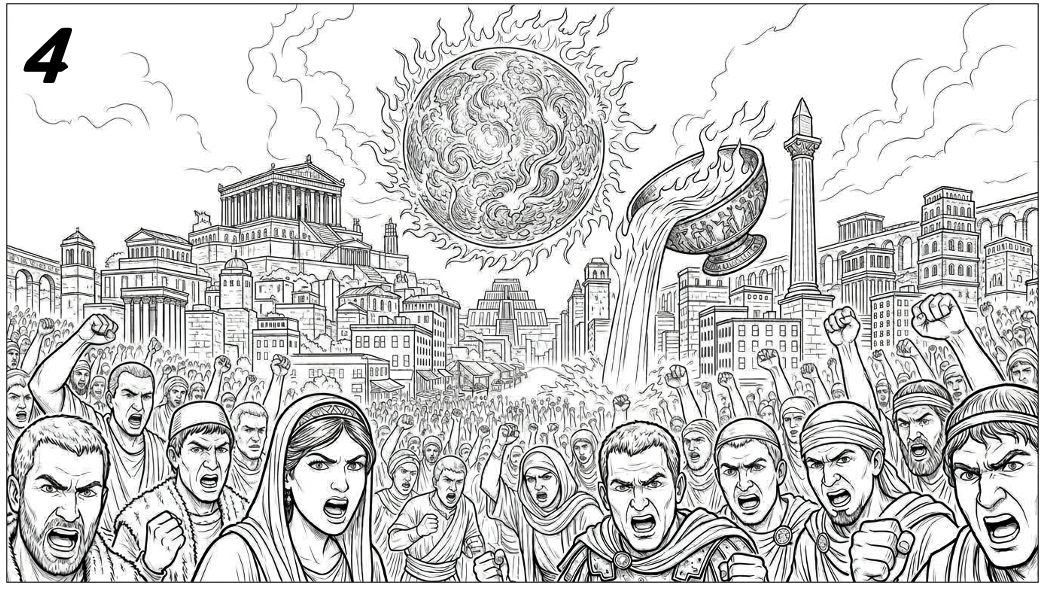
\includegraphics[
    width=1\textwidth,
    trim=0 0 0 0,
    clip]{images/bowl_4.png}
\end{figure}

At this point, we may recall the famous sermon by Jonathan Edwards, “Sinners in the Hands of an Angry God,” discussed in Chapter 10 of the first volume, \textit{Caught by Grace\index{grace}}. In forceful and unsettling language, Edwards describes the peril facing sinners who have not sought refuge in Christ:

\begin{quote}
“O sinner! Consider the fearful danger you are in: it is a great furnace of wrath, a wide and bottomless pit, full of the fire of wrath, over which you are held in the hand of that God whose wrath is provoked and incensed as much against you as against many of the damned in hell. You hang by a slender thread, with the flames of divine wrath flashing about it, ready every moment to singe it and burn it through; and you have no Mediator, no refuge to save you, no strength of your own to withstand the flames. Nothing you possess, nothing you have done, can persuade God to spare you for even a moment\ldots”
\end{quote}

Dear reader, today is still a day of grace. The Lamb has given His life for sinners. It is precisely because the coming judgment is real that the grace of God is so precious. The vision of divine wrath is not given merely to terrify us; it also summons us to seek refuge in the Savior while the invitation of grace still stands. Will you respond to God's grace and receive the salvation He offers through Christ?

\begin{ReaderQuestion}
Today is still a day of grace. How can you respond more earnestly through repentance, perseverance in faith, and trust in the Lamb? How might you share the good news of Christ with those who have not yet come to know Him?
\end{ReaderQuestion}

\begin{figure}[htbp]
    \centering
    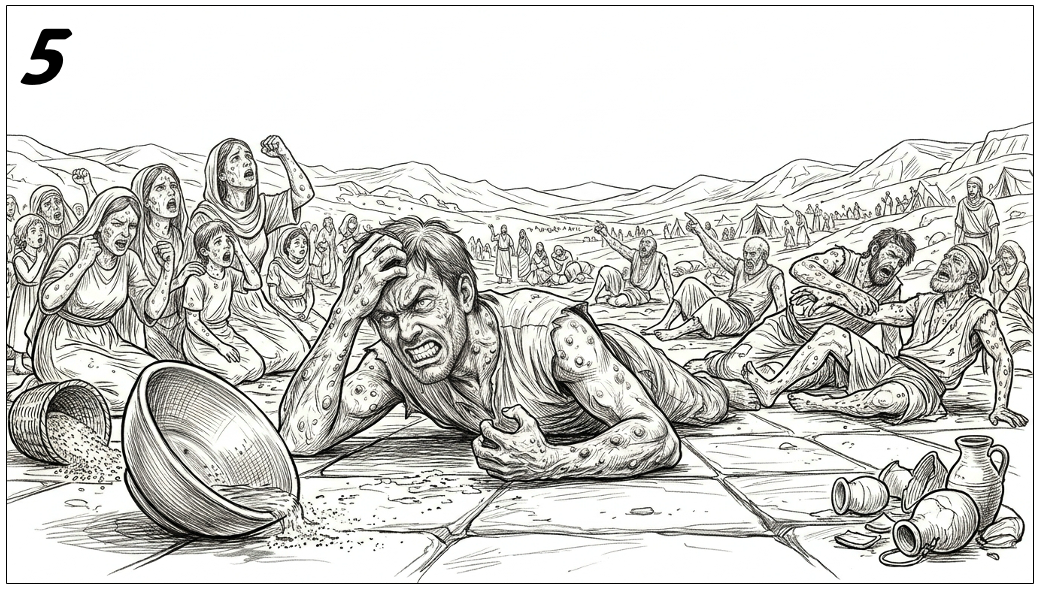
\includegraphics[
    width=1\textwidth,
    trim=0 0 0 0,
    clip]{images/bowl_5.png}
\end{figure}

\section{The Sixth Bowl}\index{bowls, seven!6@sixth bowl}

\begin{ScriptureBox2}{Out of whose mouths do the three impure spirits come, and for what do they gather the kings? What blessing does Jesus speak in 16:15?}

\item[16:12] The sixth angel poured out his bowl on the great river Euphrates, and its water was dried up to prepare the way for the kings from the East.

\item[16:13] Then I saw three impure spirits that looked like frogs; they came out of the mouth of the dragon, out of the mouth of the beast and out of the mouth of the false prophet.

\item[16:14] They are demonic spirits that perform signs, and they go out to the kings of the whole world, to gather them for the battle on the great day of God Almighty.

\item[16:15] ``Look, I come like a thief! Blessed is the one who stays awake and remains clothed, so as not to go naked and be shamefully exposed.''

\item[16:16] Then they gathered the kings together to the place that in Hebrew is called Armageddon.

\end{ScriptureBox2}

\begin{figure}[htbp]
    \centering
    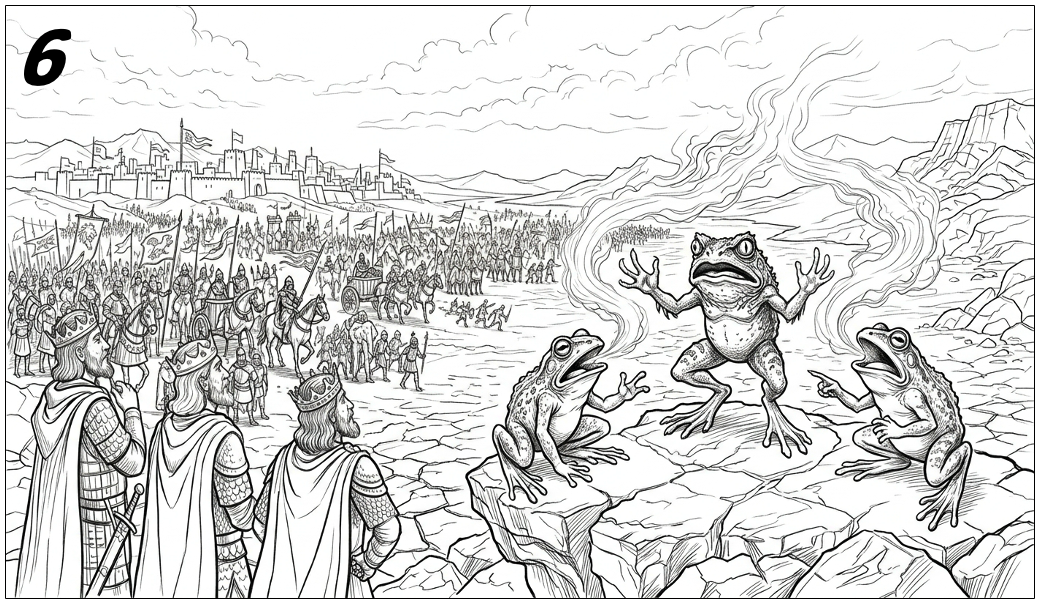
\includegraphics[
    width=1\textwidth,
    trim=0 0 0 0,
    clip]{images/bowl_6.png}
\end{figure}

Here the vision reaches one of the climactic moments of the seven bowls\index{bowls, seven}.

Three impure spirits, resembling frogs, emerge from the mouths of the dragon\index{dragon}, the beast\index{beast}, and the false prophet\index{false prophet}. They go out to deceive the kings of the earth and gather them for battle. The rulers of the nations may believe they are making their own political and military decisions. Yet John is permitted to see what lies behind the visible events: demonic spirits are deceiving them and drawing them toward the final judgment of God.

In popular novels and films about the end times\index{end times}, “Armageddon\index{Armageddon}” has become a familiar name for the great final battle. The name is generally associated with the Hebrew name Megiddo, a strategically important region in ancient Israel\index{Israel} and the site of several major conflicts. It provides a fitting symbolic setting for John's vision of the final confrontation between the powers opposed to God and the Lord who reigns over all.

Revelation 16:16 describes the gathering of the hostile earthly powers at the place called Armageddon\index{Armageddon}. The battle itself is portrayed more fully in Revelation 19:19--21. This is no contest between two evenly matched forces. Christ's victory is decisive. The forces of evil may gather in defiance of God, but they cannot overturn His sovereignty or escape His judgment.

Because the vision spans these two chapters, Figure \ref{rev_16_19_armageddon_english} presents the connection between them. It also illustrates how Satan\index{Satan} works through the three frog-like spirits to incite those who follow him on earth to oppose God. Yet Satan knows that his time is short. As Revelation 12:12 declares, his fury is great because he knows that his time is limited. His rage does not signal strength sufficient to prevail; it reveals the desperation of a defeated enemy whose end is approaching.

\begin{figure}[htbp]
    \centering
    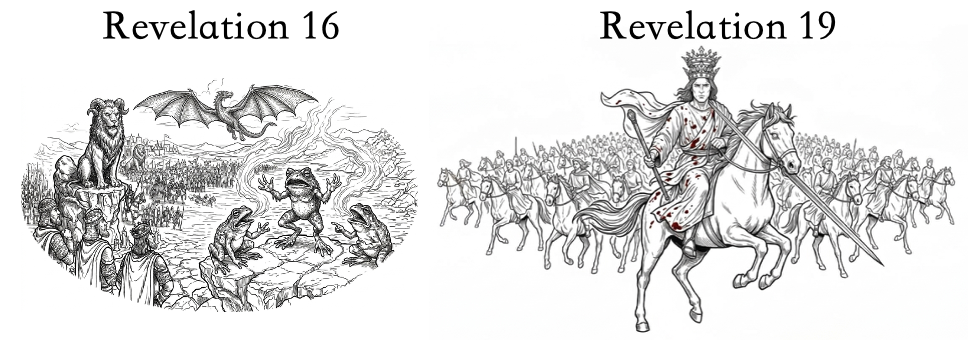
\includegraphics[
    width=1\textwidth,
    trim=0 10 20 0,
    clip]{images/rev_16_19_armageddon_english.png}
    \caption{The Battle of Armageddon}
    \label{rev_16_19_armageddon_english}
\end{figure}

\section{The Seventh Bowl}\index{bowls, seven!7@seventh bowl}

\begin{ScriptureBox2}{What does the loud voice from the throne declare? Circle every sign that follows, and notice how the people respond to the hail.}

\item[16:17] The seventh angel poured out his bowl into the air, and out of the temple came a loud voice from the throne, saying, ``It is done!''

\item[16:18] Then there came flashes of lightning, rumblings, peals of thunder and a severe earthquake. No earthquake like it has ever occurred since mankind has been on earth, so tremendous was the quake.

\item[16:19] The great city split into three parts, and the cities of the nations collapsed. God remembered Babylon the Great and gave her the cup filled with the wine of the fury of his wrath.

\item[16:20] Every island fled away and the mountains could not be found.

\item[16:21] From the sky huge hailstones, each weighing about a hundred pounds, fell on people. And they cursed God on account of the plague of hail, because the plague was so terrible.
% NIV footnote for 16:21 (omitted; add as \footnote if wanted):
%   ``a hundred pounds'' --- Or about 45 kilograms
% CHECK NIV: footnote wording quoted from memory; verify against Bible Gateway.

\end{ScriptureBox2}

The most important words in this final scene are the declaration from the throne\index{throne of God}: “It is done!” God's judgment has reached its appointed completion. Yet even as the earth is shaken to its foundations, humanity's rebellion remains stubbornly unchanged.

The earthquake\index{earthquake} is unlike any that has occurred since humanity first appeared on the earth. Hailstones weighing about a talent—approximately 45 kilograms, or 100 pounds—fall from the sky. The devastation is immense, yet the people still blaspheme God. Even in the face of overwhelming judgment, they refuse to turn to Him in repentance\index{repentance}.

This brings to mind a passage from \textit{The Great Divorce} by C. S. Lewis, quoted in Chapter 12 of the first volume, \textit{Caught by Grace}:

\begin{quote}
“There are only two kinds of people in the end: those who say to God, ‘Thy will be done,’ and those to whom God says, in the end, ‘Thy will be done.’ All that are in Hell, choose it. Without that self-choice there could be no Hell. No soul that seriously and constantly desires joy will ever miss it. Those who seek find. Those who knock it is opened.”
\footnote{Lewis, C. S. (1946). \textit{The Great Divorce}. Geoffrey Bles.}
\end{quote}

The final bowls reveal more than the destruction of the world as we know it. They expose the gravity of humanity's persistent refusal to yield to God. The question is not simply whether people will witness God's power, but whether they will humble themselves before Him. 

\begin{ReaderQuestion}
C. S. Lewis wrote that in the end there are only two kinds of people: those who say to God, ``Thy will be done,'' and those to whom God says, ``Thy will be done.'' In what area of your life are you still holding on to your own will? What would it look like to say to God today, ``Thy will be done''?
\end{ReaderQuestion}

\section*{The Seven Bowls at a Glance}\index{bowls, seven}

The following mnemonic summarizes the distinctive features of the seven bowls\index{bowls, seven} and makes them easier to remember.

{
\small
\renewcommand{\arraystretch}{1}
\begin{longtable}{>{\raggedright\arraybackslash}p{1.5cm}
                  >{\raggedright\arraybackslash}p{2cm}
                  >{\raggedright\arraybackslash}p{4cm}}
\caption{The seven bowls}
\label{tab:seven-bowls} \\
\hline
Bowl & Passage & Judgment \\
\hline
\endfirsthead

\multicolumn{3}{l}{\small\itshape Table~\thetable\ (continued)} \\
\hline
Bowl & Passage & Judgment \\
\hline
\endhead

\hline
\endfoot

\hline
\endlastfoot

First   & 16:1--2   & Sores spread \\
Second  & 16:3      & Sea red \\
Third   & 16:4--7   & Rivers bled \\
Fourth  & 16:8--9   & Sun's heat \\
Fifth   & 16:10--11 & Beast's dark seat \\
Sixth   & 16:12--16 & War begun \\
Seventh & 16:17--21 & ``It is done!'' \\
\end{longtable}
}

\chapter{Babylon Falls, and the Lamb Is Victorious (17:1--18:24)}\index{Babylon}\index{Lamb, the}

Babylon\index{Babylon} represents a world system that seduces humanity through luxury, power, and economic gain.

John sees a woman clothed in splendor, seated upon a scarlet beast. Gold, precious stones, and pearls adorn her. She has joined herself to the kings of the earth, intoxicated the nations, and enriched the merchants of the world through her extravagant wealth. Yet beneath her dazzling appearance lie corruption, idolatry, immorality, pride, and the persecution\index{persecution} of God's people. She appears powerful, prosperous, and unshakable. But God declares that her fall is certain.

The greatest danger Babylon\index{Babylon} poses is not simply her open hostility toward God, but her irresistible allure. Through wealth, success, influence, luxury, and pleasure, she persuades the world that these things constitute the glory\index{glory} for which life is meant. She does not always demand that people deny God outright. More often, she quietly teaches them to place their security in riches, measure their worth by success, entrust their hopes to power, and seek fulfillment in material abundance.

The message of Babylon\index{Babylon}, therefore, is not reserved for readers contemplating the end of the age. It speaks to every Christian who lives in the world today.

Our work, our businesses, our use of money and technology, and the resources available to us in society can all be good gifts from God. Nor can we withdraw entirely from the world in which He has placed us. The question is not whether we use these things, but whether we begin to worship\index{worship} them; not whether we possess wealth, but whether wealth has begun to possess our hearts. God does not call His people to flee the world altogether. He calls them to resist being conformed to its values.

That is why God issues His people a clear and urgent command:

“My people, come out of her, so that you will not share in her sins.” (Revelation 18:4, NIV)

Revelation places two women before our eyes: Babylon\index{Babylon}, seated upon the beast\index{beast}, and the Church, making herself ready for the Lamb\index{Lamb, the}. One embodies the splendor of the earth; the other, the glory of heaven. One appears invincible but falls in an instant; the other may seem weak in the eyes of the world, yet belongs forever to the victorious Lamb.

May we remain faithful to Christ in the midst of this world, preserving holiness amid temptation, keeping our spiritual vision clear amid material allurements, and worshiping the true King of kings\index{King of kings} even when earthly powers demand our allegiance.

\section{Babylon}\index{Babylon}

\begin{ScriptureBox2}{Circle every detail of the woman's clothing and what she holds. What is written on her forehead, and what is she drunk with?}

\item[17:1] One of the seven angels who had the seven bowls came and said to me, ``Come, I will show you the punishment of the great prostitute, who sits by many waters.

\item[17:2] With her the kings of the earth committed adultery, and the inhabitants of the earth were intoxicated with the wine of her adulteries.''

\item[17:3] Then the angel carried me away in the Spirit into a wilderness. There I saw a woman sitting on a scarlet beast that was covered with blasphemous names and had seven heads and ten horns.

\item[17:4] The woman was dressed in purple and scarlet, and was glittering with gold, precious stones and pearls. She held a golden cup in her hand, filled with abominable things and the filth of her adulteries.

\item[17:5] The name written on her forehead was a mystery:\\
\hspace*{1em}\textsc{Babylon the Great}\\
\hspace*{1em}\textsc{the mother of prostitutes}\\
\hspace*{1em}\textsc{and of the abominations of the earth.}

\item[17:6] I saw that the woman was drunk with the blood of God's holy people, the blood of those who bore testimony to Jesus.\\
When I saw her, I was greatly astonished.

\item[17:7] Then the angel said to me: ``Why are you astonished? I will explain to you the mystery of the woman and of the beast she rides, which has the seven heads and ten horns.

\item[17:8] The beast, which you saw, once was, now is not, and yet will come up out of the Abyss and go to its destruction. The inhabitants of the earth whose names have not been written in the book of life from the creation of the world will be astonished when they see the beast, because it once was, now is not, and yet will come.

\end{ScriptureBox2}

\begin{figure}[htbp]
    \centering
    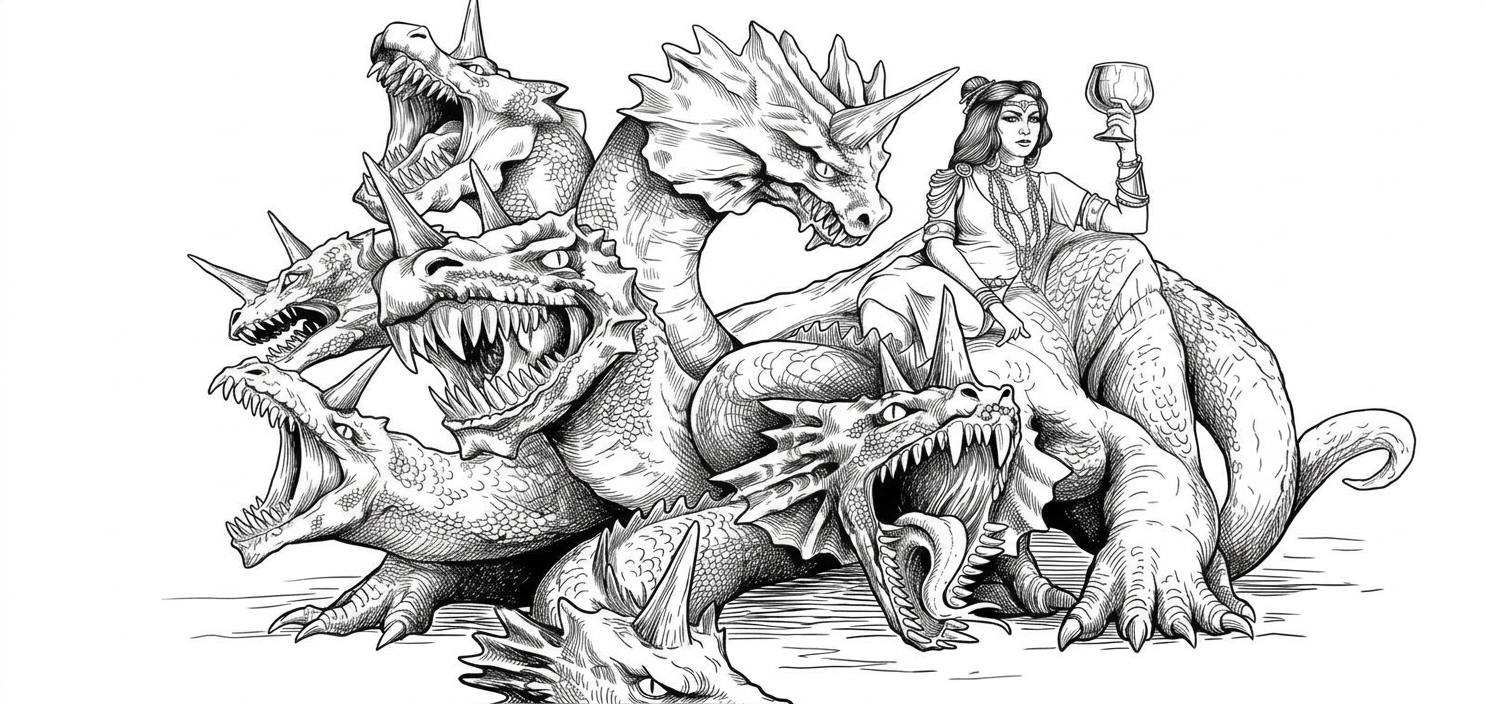
\includegraphics[
    width=1\textwidth,
    trim=0 0 0 0,
    clip]{images/babylon_harlot.jpg}
    %\caption{}
    %\label{}
\end{figure}

\begin{ScriptureBox2}{What do the seven heads, the ten horns, and the waters stand for? Underline who will triumph in 17:14, and why.}

\item[17:9] ``This calls for a mind with wisdom. The seven heads are seven hills on which the woman sits.

\item[17:10] They are also seven kings. Five have fallen, one is, the other has not yet come; but when he does come, he must remain for only a little while.

\item[17:11] The beast who once was, and now is not, is an eighth king. He belongs to the seven and is going to his destruction.

\item[17:12] ``The ten horns you saw are ten kings who have not yet received a kingdom, but who for one hour will receive authority as kings along with the beast.

\item[17:13] They have one purpose and will give their power and authority to the beast.

\item[17:14] They will wage war against the Lamb, but the Lamb will triumph over them because he is Lord of lords and King of kings---and with him will be his called, chosen and faithful followers.''

\item[17:15] Then the angel said to me, ``The waters you saw, where the prostitute sits, are peoples, multitudes, nations and languages.

\item[17:16] The beast and the ten horns you saw will hate the prostitute. They will bring her to ruin and leave her naked; they will eat her flesh and burn her with fire.

\item[17:17] For God has put it into their hearts to accomplish his purpose by agreeing to hand over to the beast their royal authority, until God's words are fulfilled.

\item[17:18] The woman you saw is the great city that rules over the kings of the earth.''

\end{ScriptureBox2}

“Babylon\index{Babylon}” may be understood as Rome\index{Rome} in the first century, or more broadly as the world system that sets itself against God. Accordingly, interpreters throughout the centuries have offered different explanations of the identities of Babylon and the ten kings.

The following table summarizes several major interpretations of the ten kings:

{
\renewcommand{\arraystretch}{1}
\small
\begin{longtable}{>{\raggedright\arraybackslash}p{3.6cm}
                  >{\raggedright\arraybackslash}p{5.4cm}}
\caption{Interpretations of the ten kings (Revelation 17)}
\label{tab:ten-kings} \\
\hline
Interpretation of the Ten Kings & Principal Basis \\
\hline
\endfirsthead

\multicolumn{2}{l}{\small\itshape Table~\thetable\ (continued)} \\
\hline
Interpretation of the Ten Kings & Principal Basis \\
\hline
\endhead

\hline
\endfoot

\hline
\endlastfoot

An alliance of ten political powers at the end of the age &
Revelation 17:12--13, which describes ten kings who receive authority with the beast for a brief time. \\

Ten emperors in the history of first-century Rome &
Revelation 17:10: ``Five have fallen, one is, the other has not yet come.'' \\

Empires drawn from the visions of Daniel &
Emphasizes the background of the four beasts and the ten horns in Daniel 7. \\

Symbolic political powers &
Emphasizes the symbolic language of Revelation; the ten kings need not represent ten individually identifiable rulers. \\

\end{longtable}
}

Whichever interpretation one adopts, the central message of this chapter remains unchanged. These earthly powers will ultimately wage war against the Lamb, but “the Lamb will triumph over them because he is Lord of lords and King of kings\index{King of kings}.” Earthly rulers may gather their authority, unite their ambitions, and set themselves against God's kingdom. Yet their combined power cannot overturn the reign of the Lamb.

\section{Come Out of Her, My People, So That You Will Not Share in Her Sins}

\begin{ScriptureBox2}{Underline the command God gives His people in 18:4. Then circle the three groups who weep and mourn over Babylon. What exactly do they mourn?}

\item[18:1] After this I saw another angel coming down from heaven. He had great authority, and the earth was illuminated by his splendor.

\item[18:2] With a mighty voice he shouted:\\
\hspace*{1em}``\,`Fallen! Fallen is Babylon the Great!'\\
\hspace*{2em}She has become a dwelling for demons\\
\hspace*{1em}and a haunt for every impure spirit,\\
\hspace*{2em}a haunt for every unclean bird,\\
\hspace*{2em}a haunt for every unclean and detestable animal.
% NIV footnote for 18:2: ``Fallen is Babylon the Great!'' --- Isaiah 21:9

\item[18:3] \hspace*{1em}For all the nations have drunk\\
\hspace*{2em}the maddening wine of her adulteries.\\
\hspace*{1em}The kings of the earth committed adultery with her,\\
\hspace*{2em}and the merchants of the earth grew rich from her excessive luxuries.''

\item[18:4] Then I heard another voice from heaven say:\\
\hspace*{1em}``\,`Come out of her, my people,'\\
\hspace*{2em}so that you will not share in her sins,\\
\hspace*{2em}so that you will not receive any of her plagues;
% NIV footnote for 18:4: ``Come out of her, my people'' --- Jer. 51:45

\item[18:5] \hspace*{1em}for her sins are piled up to heaven,\\
\hspace*{2em}and God has remembered her crimes.

\item[18:6] \hspace*{1em}Give back to her as she has given;\\
\hspace*{2em}pay her back double for what she has done.\\
\hspace*{2em}Pour her a double portion from her own cup.

\item[18:7] \hspace*{1em}Give her as much torment and grief\\
\hspace*{2em}as the glory and luxury she gave herself.\\
\hspace*{1em}In her heart she boasts,\\
\hspace*{2em}`I sit enthroned as queen.\\
\hspace*{1em}I am not a widow;\\
\hspace*{2em}I will never mourn.'
% NIV footnote for 18:7: ``I am not a widow'' --- Isaiah 47:7,8

\item[18:8] \hspace*{1em}Therefore in one day her plagues will overtake her:\\
\hspace*{2em}death, mourning and famine.\\
\hspace*{1em}She will be consumed by fire,\\
\hspace*{2em}for mighty is the Lord God who judges her.

\item[18:9] ``When the kings of the earth who committed adultery with her and shared her luxury see the smoke of her burning, they will weep and mourn over her.

\item[18:10] Terrified at her torment, they will stand far off and cry:\\
\hspace*{1em}``\,`Woe! Woe to you, great city,\\
\hspace*{2em}you mighty city of Babylon!\\
\hspace*{1em}In one hour your doom has come!'

\item[18:11] ``The merchants of the earth will weep and mourn over her because no one buys their cargoes anymore---

\item[18:12] cargoes of gold, silver, precious stones and pearls; fine linen, purple, silk and scarlet cloth; every sort of citron wood, and articles of every kind made of ivory, costly wood, bronze, iron and marble;

\item[18:13] cargoes of cinnamon and spice, of incense, myrrh and frankincense, of wine and olive oil, of fine flour and wheat; cattle and sheep; horses and carriages; and human beings sold as slaves.

\item[18:14] ``They will say, `The fruit you longed for is gone from you. All your luxury and splendor have vanished, never to be recovered.'

\item[18:15] The merchants who sold these things and gained their wealth from her will stand far off, terrified at her torment. They will weep and mourn

\item[18:16] and cry out:\\
\hspace*{1em}``\,`Woe! Woe to you, great city,\\
\hspace*{2em}dressed in fine linen, purple and scarlet,\\
\hspace*{2em}and glittering with gold, precious stones and pearls!

\item[18:17] \hspace*{1em}In one hour such great wealth has been brought to ruin!'\\
``Every sea captain, and all who travel by ship, the sailors, and all who earn their living from the sea, will stand far off.

\item[18:18] When they see the smoke of her burning, they will exclaim, `Was there ever a city like this great city?'

\item[18:19] They will throw dust on their heads, and with weeping and mourning cry out:\\
\hspace*{1em}``\,`Woe! Woe to you, great city,\\
\hspace*{2em}where all who had ships on the sea\\
\hspace*{2em}became rich through her wealth!\\
\hspace*{1em}In one hour she has been brought to ruin!'

\item[18:20] \hspace*{1em}``Rejoice over her, you heavens!\\
\hspace*{2em}Rejoice, you people of God!\\
\hspace*{2em}Rejoice, apostles and prophets!\\
\hspace*{1em}For God has judged her\\
\hspace*{2em}with the judgment she imposed on you.''

\item[18:21] Then a mighty angel picked up a boulder the size of a large millstone and threw it into the sea, and said:\\
\hspace*{1em}``With such violence\\
\hspace*{2em}the great city of Babylon will be thrown down,\\
\hspace*{2em}never to be found again.

\item[18:22] \hspace*{1em}The music of harpists and musicians, pipers and trumpeters,\\
\hspace*{2em}will never be heard in you again.\\
\hspace*{1em}No worker of any trade\\
\hspace*{2em}will ever be found in you again.\\
\hspace*{1em}The sound of a millstone\\
\hspace*{2em}will never be heard in you again.

\item[18:23] \hspace*{1em}The light of a lamp\\
\hspace*{2em}will never shine in you again.\\
\hspace*{1em}The voice of bridegroom and bride\\
\hspace*{2em}will never be heard in you again.\\
\hspace*{1em}Your merchants were the world's important people.\\
\hspace*{2em}By your magic spell all the nations were led astray.

\item[18:24] \hspace*{1em}In her was found the blood of prophets and of God's holy people,\\
\hspace*{2em}of all who have been slaughtered on the earth.''
% CHECK NIV: footnote references for 18:2, 18:4, 18:7 quoted from memory;
%   verify against Bible Gateway.

\end{ScriptureBox2}

The kings of the earth and the merchants behold Babylon\index{Babylon}'s sudden destruction and break into lamentation. In a single day, the great city that seemed so wealthy and secure is brought down and consumed by fire.

This is the climax of the judgments\index{judgment} revealed through the seven seals\index{seals, seven}, seven trumpets\index{trumpets, seven}, and seven bowls\index{bowls, seven}. The world that trusted in Babylon\index{Babylon}'s strength is confronted with the fragility of everything it has built. Yet the kings and merchants do not mourn primarily for their own peril. They weep for the treasures they have lost, the markets that have vanished, and the luxuries they can no longer enjoy.

Their grief exposes the depths of their attachment to wealth. Even as judgment approaches and their own lives stand in jeopardy, they mourn the loss of their possessions rather than reckon with the condition of their souls. Their treasures have so captured their hearts that they cannot see beyond them, even at the threshold of judgment.

\begin{ReaderQuestion}
Babylon appears magnificent and prosperous, yet she is filled with corruption and persecutes God's people. How does this contrast warn us against judging a society or system solely by its outward prosperity?
\end{ReaderQuestion}

\begin{figure}[htbp]
    \centering
    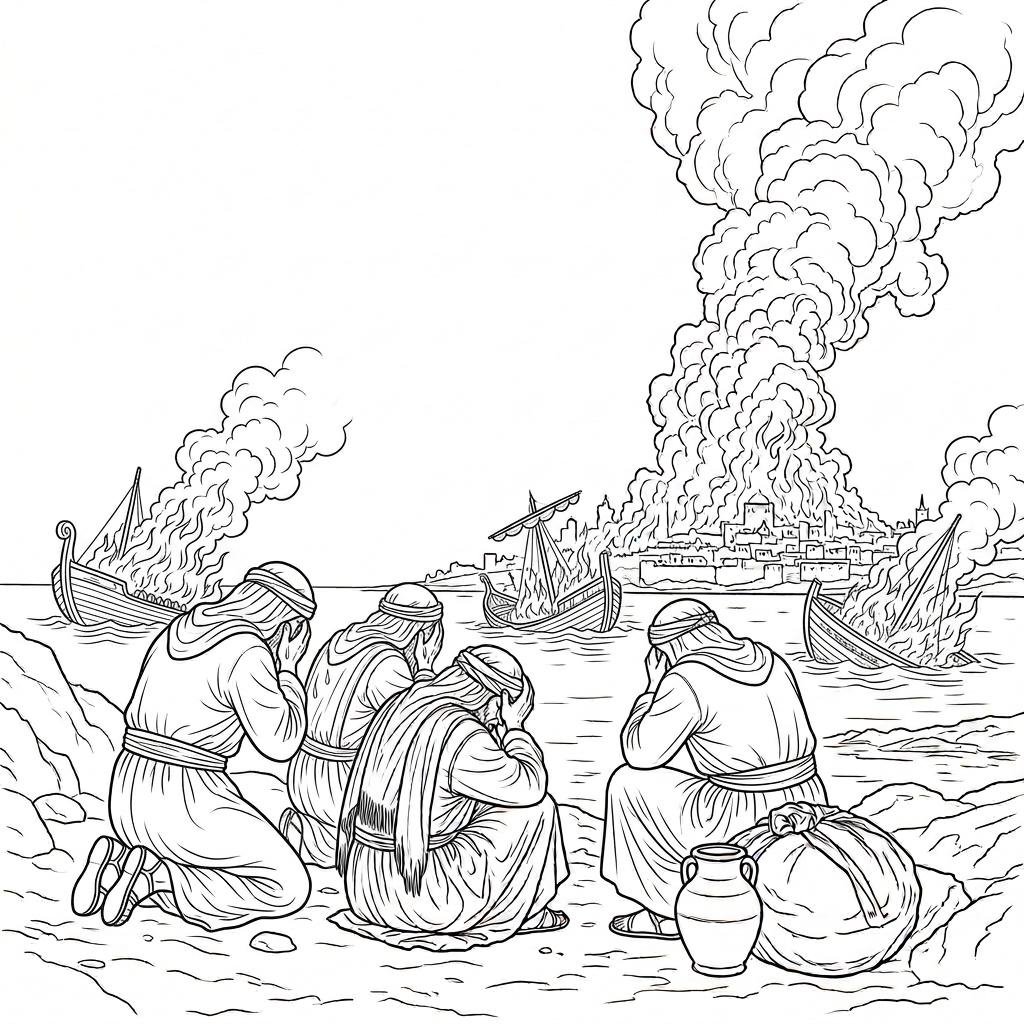
\includegraphics[
    width=0.9\textwidth,
    trim=0 0 0 0,
    clip]{images/rev_18_bablyon_burning.jpg}
    %\caption{}
    %\label{}
\end{figure}

The beast\index{beast} represents the power that opposes God. The ten horns\index{seven heads and ten horns} represent ten kings who unite with the beast. Babylon\index{Babylon}, portrayed as the great prostitute\index{great prostitute}, symbolizes a world system that seduces the nations through luxury, power, and economic gain. Bound together by shared interests, these powers surrender their authority to the beast and unite in opposition to the Lamb.

Yet their alliance does not endure. In the end, the ten horns\index{seven heads and ten horns} and the beast turn against the prostitute\index{great prostitute} herself. They strip her, devastate her, and consume her with fire. Their hostility reveals the instability of a kingdom built upon rebellion and self-interest. The forces opposed to God may form alliances for a season, but they cannot establish an everlasting order. God remains sovereign over history, even turning their mutual hatred against one another to accomplish His judgment.

For the early Church, Babylon\index{Babylon}'s downfall presented a choice with immediate and personal consequences. Rome\index{Rome} commanded formidable political power, controlled an extensive network of trade, and possessed extraordinary material wealth. Through imperial worship and other public expressions of loyalty, it also asserted its authority over the lives and consciences of its subjects.

When society demanded that Christians participate in idolatrous practices or express allegiance to the emperor and earthly powers in ways that contradicted their faith, they had to choose: Would they conform to the expectations of the surrounding world, or remain loyal to Jesus Christ?

\begin{ReaderQuestion}
God declares, “Come out of her, my people, so that you will not share in her sins.” What did this command mean for the early Church? What does it call the Church today to examine in its own life and witness?
\end{ReaderQuestion}

The contrast becomes even more striking when we compare Babylon\index{Babylon}, the prostitute\index{great prostitute} of Revelation 17 and 18, with the bride\index{bride of the Lamb} of the Lamb in Revelation 21. Table \ref{tab:babylon_bride} sets these two visions side by side.
{
\small
\renewcommand{\arraystretch}{1}
\begin{longtable}{>{\raggedright\arraybackslash}p{2.2cm}
                  >{\raggedright\arraybackslash}p{3.4cm}
                  >{\raggedright\arraybackslash}p{3.4cm}}
\caption{The Bride of the Holy City Is Beyond Compare}
\label{tab:babylon_bride} \\
\hline
Contrast & Babylon, the Prostitute (Chapter 18) & The Bride of the Holy City (Chapter 21) \\
\hline
\endfirsthead

\multicolumn{3}{l}{\small\itshape Table~\thetable\ (continued)} \\
\hline
Contrast & Babylon, the Prostitute (Chapter 18) & The Bride of the Holy City (Chapter 21) \\
\hline
\endhead

\hline
\endfoot

\hline
\endlastfoot

Passages &
17:1--6; 18:1--24 &
21:2, 9--10 \\

Symbolism &
A world system that seduces the nations. &
God's people, redeemed by the Lamb. \\

Outward appearance &
Clothed in purple and scarlet, adorned with gold, precious stones, and pearls. &
The city shines with the glory of God, radiant like a precious jewel (21:11). \\

Relationship with the nations &
The kings of the earth commit adultery with her. &
The kings of the earth bring their glory into the city (21:24--26). \\

Relationship with God &
Filled with abominations and stained with the blood of the saints. &
God's dwelling is among His people, and He lives with them (21:3). \\

Relationship with humanity &
Merchants grow rich through her extravagant luxury (18:3, 15--19). &
God freely gives the water of life to the thirsty (21:6, 17). \\

Tears and death &
The world mourns her destruction (18:9--19). &
God wipes away every tear; death, mourning, crying, and pain are no more (21:4). \\

Final destiny &
Destroyed and cast down (18:8--10, 21). &
Descends from heaven, to dwell with God and His people forever (21:2--3). \\

\end{longtable}
}

Babylon\index{Babylon} dazzles the world with splendor that cannot endure. The holy city\index{holy city} shines with a glory that comes from God and will never fade. Babylon enriches merchants, seduces rulers, and sheds the blood of the faithful; the New Jerusalem\index{New Jerusalem} welcomes God's redeemed\index{redemption} people into His presence. Babylon's admirers weep because their earthly treasures have vanished. In the holy city, God Himself wipes away every tear.

The contrast reaches beyond two cities or two women. It reveals two rival visions of glory. One seeks to ascend through wealth, domination, and self-exaltation, only to fall. The other receives its glory from God, belongs to the Lamb, and endures forever. The Christian life is shaped by the choice between them: to be captivated by what dazzles for a moment, or to remain faithful to the One whose kingdom has no end.

\begin{ReaderQuestion}
In what ways might believers today be drawn toward Babylon's values---wealth, success, power, pleasure, or human approval? How can we examine our hearts and recognize when these things are beginning to take God's place?
\end{ReaderQuestion}

\chapter{The Invitation to the Banquet (19:1--19:21)}

Revelation 19 brings us before two very different banquets. The first is the wedding supper\index{wedding supper of the Lamb} of the Lamb\index{Lamb, the}: “Blessed are those who are invited to the wedding supper of the Lamb.” The bride\index{bride of the Lamb} has made herself ready, and heaven resounds with praise. This is the feast of the Lamb and His people, a celebration of salvation, joy, and eternal fellowship.

The second is “the great banquet\index{great banquet of God} of God.” Here, the birds of the sky are summoned to feast upon the flesh of those who have set themselves against God. It is a dreadful counterpart to the wedding supper\index{wedding supper of the Lamb}—a vision of judgment\index{judgment} upon the enemies of the Lord.

Then Christ appears, riding upon a white horse\index{white horse}. He is called “Faithful and True.” In righteousness He judges and wages war, overthrowing the beast\index{beast} and the false prophet\index{false prophet}. The Christ whom the world once rejected and persecuted\index{persecution} now reveals His glory\index{glory} in full. Before Him, every power that opposes God is brought to nothing.

Even today, the Lamb extends His invitation. May we receive His grace\index{grace} by faith, follow Him with steadfast hearts, and make ourselves ready to welcome the King who is coming again.

\section{The Wedding Supper of the Lamb}\index{wedding supper of the Lamb}\index{Lamb, the}

\begin{ScriptureBox2}{Count how many times ``Hallelujah'' appears. Why does the multitude praise God, and what is the bride given to wear?}

\item[19:1] After this I heard what sounded like the roar of a great multitude in heaven shouting:\\
\hspace*{1em}``Hallelujah!\\
\hspace*{1em}Salvation and glory and power belong to our God,

\item[19:2] \hspace*{2em}for true and just are his judgments.\\
\hspace*{1em}He has condemned the great prostitute\\
\hspace*{2em}who corrupted the earth by her adulteries.\\
\hspace*{1em}He has avenged on her the blood of his servants.''

\item[19:3] And again they shouted:\\
\hspace*{1em}``Hallelujah!\\
\hspace*{1em}The smoke from her goes up for ever and ever.''

\item[19:4] The twenty-four elders and the four living creatures fell down and worshiped God, who was seated on the throne. And they cried:\\
\hspace*{1em}``Amen, Hallelujah!''

\item[19:5] Then a voice came from the throne, saying:\\
\hspace*{1em}``Praise our God,\\
\hspace*{2em}all you his servants,\\
\hspace*{1em}you who fear him,\\
\hspace*{2em}both great and small!''

\item[19:6] Then I heard what sounded like a great multitude, like the roar of rushing waters and like loud peals of thunder, shouting:\\
\hspace*{1em}``Hallelujah!\\
\hspace*{2em}For our Lord God Almighty reigns.

\item[19:7] \hspace*{1em}Let us rejoice and be glad\\
\hspace*{2em}and give him glory!\\
\hspace*{1em}For the wedding of the Lamb has come,\\
\hspace*{2em}and his bride has made herself ready.

\item[19:8] \hspace*{1em}Fine linen, bright and clean,\\
\hspace*{2em}was given her to wear.''\\
(Fine linen stands for the righteous acts of God's holy people.)

\item[19:9] Then the angel said to me, ``Write this: Blessed are those who are invited to the wedding supper of the Lamb!'' And he added, ``These are the true words of God.''

\item[19:10] At this I fell at his feet to worship him. But he said to me, ``Don't do that! I am a fellow servant with you and with your brothers and sisters who hold to the testimony of Jesus. Worship God! For it is the Spirit of prophecy who bears testimony to Jesus.''

\end{ScriptureBox2}

The great multitude\index{great multitude} in heaven praises God because His judgments are true and righteous. His justice has been fully revealed, and heaven responds with worship\index{worship}. Among those whose long-awaited vindication is now proclaimed are the martyrs\index{martyrs} we encountered in Revelation 6:10. Beneath the altar\index{altar}, they had cried out, “How long, Sovereign Lord, holy and true, until you judge the inhabitants of the earth and avenge our blood?”

Their question had risen from the suffering of the faithful, whose lives were taken because of their testimony to God. Now, the heavenly chorus declares that their cries have not been forgotten. God's apparent delay was never indifference, and His silence was never the absence of justice. At the appointed time, He judges evil and vindicates His servants.

The scene then turns from the judgment of Babylon\index{Babylon} to the joy of the Lamb's wedding supper\index{wedding supper of the Lamb}. The bride\index{bride of the Lamb} has made herself ready, clothed in fine linen, bright and clean. Yet even this garment is received by grace. The vision identifies the linen with the righteous deeds of God's holy people: their faithful lives are the fruit of belonging to the Lamb. Their readiness is not a claim to glory apart from Him, but the visible expression of a life redeemed\index{redemption} by His grace.

The angel commands John to write down the blessing: those invited to the wedding supper\index{wedding supper of the Lamb} of the Lamb are blessed indeed. This is God's sure promise. The history of the world does not end with the mourning of Babylon\index{Babylon}'s merchants or the defeat of the saints. It moves toward the joyous fellowship of the Lamb and His redeemed people.

\begin{ReaderQuestion}
Revelation 19:9 declares, “Blessed are those who are invited to the wedding supper of the Lamb.” If we truly believe that we have been invited to this supper, how should that assurance shape the way we live today?
\end{ReaderQuestion}

\section{Christ on the White Horse: King of Kings}\index{King of kings}\index{white horse}

\begin{figure}[htbp]
    \centering
    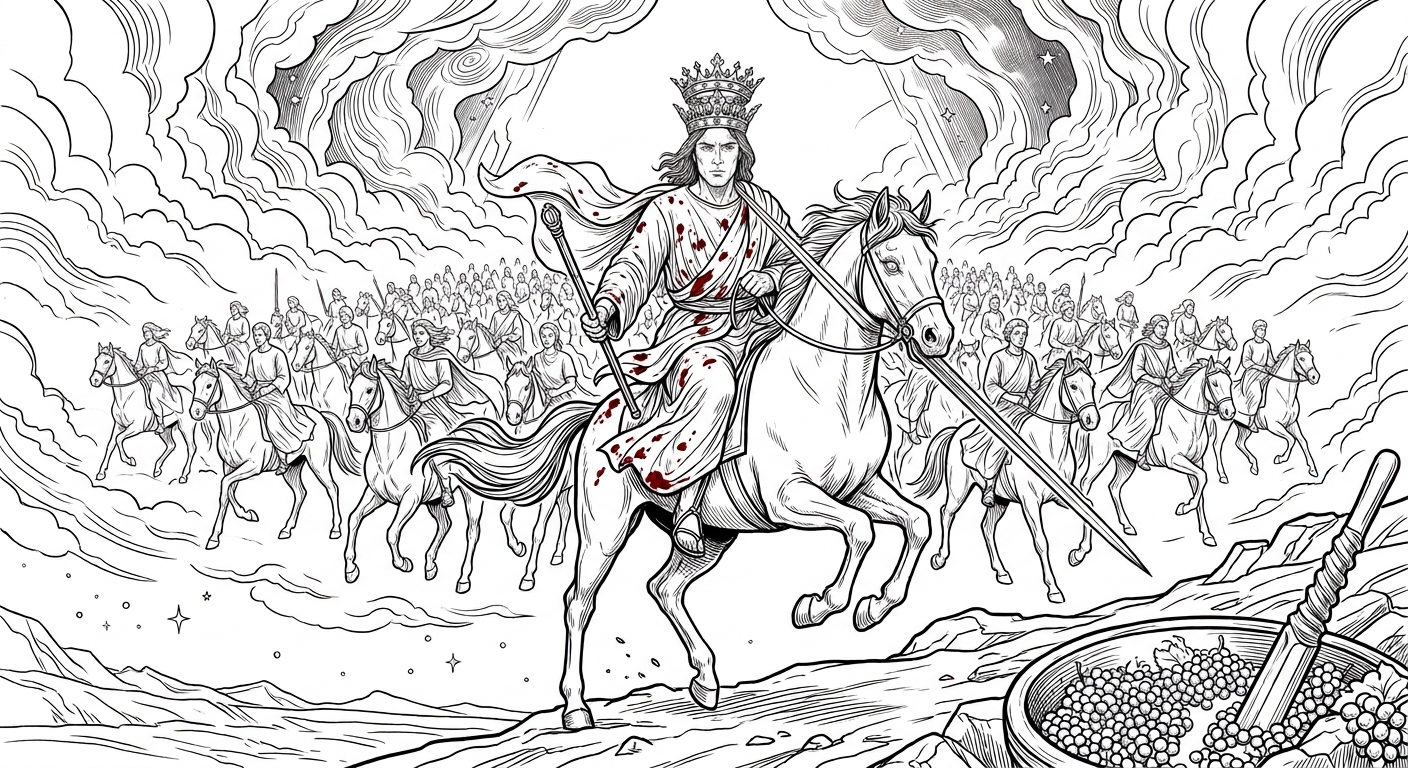
\includegraphics[
    width=1\textwidth,
    trim=0 0 0 0,
    clip]{images/christ_blood_white_horse.jpg}
    %\caption{}
    %\label{}
\end{figure}

\begin{ScriptureBox2}{Circle every name and title given to the rider on the white horse. What is He wearing, and what comes out of His mouth?}

\item[19:11] I saw heaven standing open and there before me was a white horse, whose rider is called Faithful and True. With justice he judges and wages war.

\item[19:12] His eyes are like blazing fire, and on his head are many crowns. He has a name written on him that no one knows but he himself.

\item[19:13] He is dressed in a robe dipped in blood, and his name is the Word of God.

\item[19:14] The armies of heaven were following him, riding on white horses and dressed in fine linen, white and clean.

\item[19:15] Coming out of his mouth is a sharp sword with which to strike down the nations. ``He will rule them with an iron scepter.'' He treads the winepress of the fury of the wrath of God Almighty.
% NIV footnote for 19:15 (omitted; add as \footnote if wanted):
%   ``with an iron scepter'' --- Psalm 2:9
% CHECK NIV: footnote reference quoted from memory; verify against Bible Gateway.

\item[19:16] On his robe and on his thigh he has this name written:\\
\hspace*{1em}\textsc{king of kings and lord of lords.}

\end{ScriptureBox2}

John sees heaven opened and a white horse\index{white horse} appear, with Christ seated upon it. This is not the white horse of Revelation 6. Here, the rider is unmistakably revealed in His royal glory. He is Faithful and True, and He judges and wages war in righteousness. His eyes blaze like fire, and many crowns rest upon His head. His name is the Word of God, and upon His robe and thigh is written the title that declares His supreme authority: King of kings\index{King of kings} and Lord of lords.

His robe is stained with blood. The image evokes the terrible reality of divine judgment, while also recalling the blood through which Christ redeemed His people. The One who comes to judge is the same Lord who gave Himself for sinners. He is not merely another earthly conqueror\index{overcomers}, nor is His victory uncertain. The armies of heaven follow Him, but the decisive power belongs to the King Himself. The sword proceeds from His mouth, signifying the authority of His word to judge the nations.

The world once treated Christ as one who could be rejected, condemned, and crucified. Yet the risen Lord now appears in the majesty that was His all along. The powers of the earth may gather against Him, but no throne\index{throne of God} can rival His throne, no crown can surpass His crown, and no kingdom can withstand His reign. He is the King of kings\index{King of kings} and the Lord of lords.

\begin{ReaderQuestion}
What names and images are used to describe Christ in Revelation 19:11--16? What do the titles “Faithful and True,” “the Word of God,” and “King of kings and Lord of lords” teach you about Him?
\end{ReaderQuestion}

\section{The Great Banquet of God}\index{great banquet of God}

\begin{ScriptureBox2}{Who is invited to the great supper of God? What happens to the beast and the false prophet, and what happens to the rest?}

\item[19:17] And I saw an angel standing in the sun, who cried in a loud voice to all the birds flying in midair, ``Come, gather together for the great supper of God,

\item[19:18] so that you may eat the flesh of kings, generals, and the mighty, of horses and their riders, and the flesh of all people, free and slave, great and small.''

\item[19:19] Then I saw the beast and the kings of the earth and their armies gathered together to wage war against the rider on the horse and his army.

\item[19:20] But the beast was captured, and with it the false prophet who had performed the signs on its behalf. With these signs he had deluded those who had received the mark of the beast and worshiped its image. The two of them were thrown alive into the fiery lake of burning sulfur.

\item[19:21] The rest were killed with the sword coming out of the mouth of the rider on the horse, and all the birds gorged themselves on their flesh.

\end{ScriptureBox2}

In this chapter, Revelation places two banquets side by side: the wedding supper\index{wedding supper of the Lamb} of the Lamb and the great banquet\index{great banquet of God} of God. The contrast could hardly be more striking. The wedding supper celebrates the salvation and joy shared by Christ and His people; the great banquet portrays the final judgment awaiting the powers that oppose God.

An angel standing in the sun calls to the birds flying overhead, summoning them to gather for God's great banquet\index{great banquet of God}. The imagery is stark and unsettling. The kings of the earth, their generals, their warriors, and people of every rank have assembled to wage war against the rider on the white horse\index{white horse} and His army. Yet the outcome is not a contest between equally matched forces. The beast\index{beast} and the false prophet\index{false prophet} are captured and thrown alive into the fiery lake of burning sulfur. The rest are struck down by the sword that comes from the rider's mouth, and the birds gorge themselves on their flesh.

The gathering intended as a show of defiance becomes the scene of utter defeat. The beast, which deceived the nations through its signs and falsehoods, cannot save itself. The earthly kings who placed their confidence in its power cannot rescue it. Their weapons, alliances, and ambitions prove powerless before Christ.

The two banquets therefore reveal two radically different destinies. Those who belong to the Lamb are welcomed into the joy of His eternal kingdom. Those who persist in rebellion against God face His righteous judgment. The invitation of grace and the warning of judgment stand before the reader together. Revelation calls us not merely to observe these visions, but to consider where our own allegiance lies.

The final victory belongs to Christ. The Lamb who was slain\index{Lamb, the!slain} is the King who reigns; the Savior who calls His people to the wedding supper\index{wedding supper of the Lamb} is the Judge before whom every enemy must answer. Blessed are those who belong to Him, who remain faithful to His testimony, and who await His coming with hope.

\begin{ReaderQuestion}
If you were reading Revelation 19 in the midst of suffering, temptation, or uncertainty, which truth would most strengthen your faith: God's true and righteous judgment, the wedding supper of the Lamb, Christ's sovereignty as King of kings, or the Lamb's final victory? Why?
\end{ReaderQuestion}

\chapter{Christ Defeats Satan (20:1--20:15)}\index{Satan}

The twentieth chapter brings us at last before the great white throne\index{great white throne}. On that day, every person will stand before God. No one, great or small, will escape the final judgment\index{judgment}, regardless of the power, wealth, or renown they possessed in this world. Neither death nor Hades\index{Hades} can offer a permanent refuge. The books will be opened, and every life will be laid bare before God.

This chapter has also been interpreted in different ways. Is the thousand years a literal period of a thousand years, or does it symbolize a complete span of time? Does the ``first resurrection\index{first resurrection}'' refer to the resurrection of the body or to spiritual life? Will Christ reign on earth for a thousand years, or is He already reigning? What does it mean for Satan\index{Satan} to be bound? Generations of Christians have wrestled seriously with these questions, giving rise to different positions on the end times\index{end times}.

Yet as we read this chapter, we must not allow these questions to obscure what John most wants us to see. Satan\index{Satan} is not the final King. Christ is. And the question we must ask ourselves is this: ``Since Christ will surely triumph, how should I faithfully follow Him today?''

\section{Satan Bound, the Saints Reigning with Christ}\index{Satan}

\begin{figure}[htbp]
    \centering
    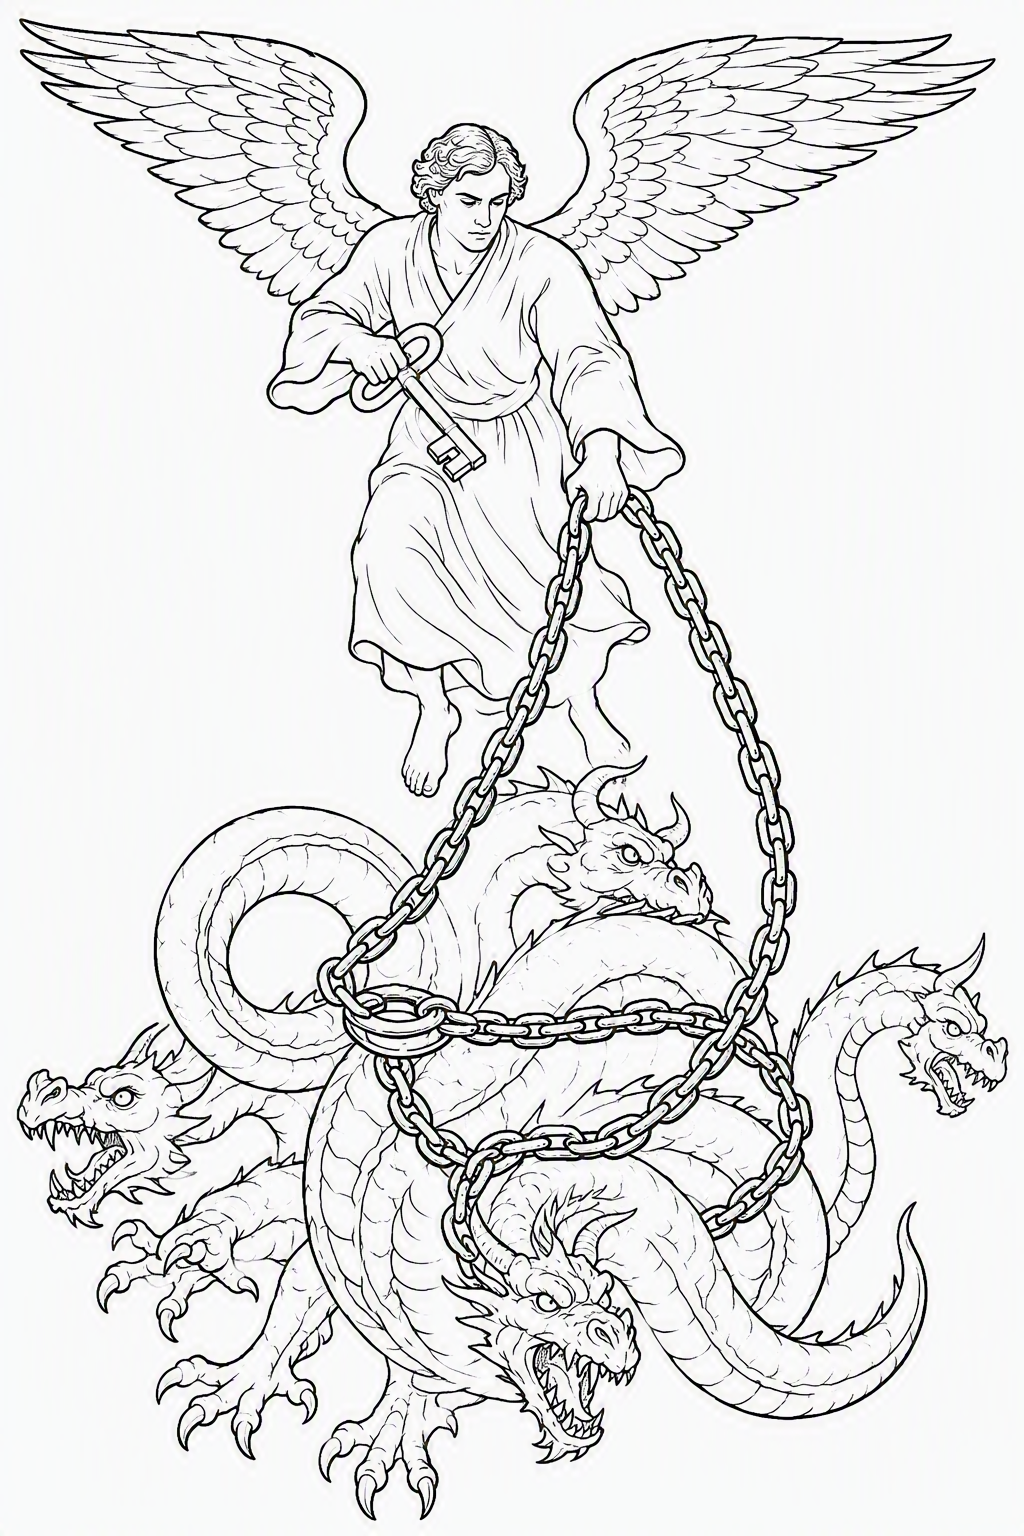
\includegraphics[
    width=0.6\textwidth,
    trim=0 0 0 0,
    clip]{images/rev20-satan-bound.png}
\end{figure}

\begin{ScriptureBox}

\item[20:1] And I saw an angel coming down out of heaven, having the key to the Abyss and holding in his hand a great chain.

\item[20:2] He seized the dragon, that ancient serpent, who is the devil, or Satan, and bound him for a thousand years.

\item[20:3] He threw him into the Abyss, and locked and sealed it over him, to keep him from deceiving the nations anymore until the thousand years were ended. After that, he must be set free for a short time.

\item[20:4] I saw thrones on which were seated those who had been given authority to judge. And I saw the souls of those who had been beheaded because of their testimony about Jesus and because of the word of God. They had not worshiped the beast or its image and had not received its mark on their foreheads or their hands. They came to life and reigned with Christ a thousand years.
% NIV footnote for 20:4 (omitted; add as \footnote if wanted):
%   ``They'' --- Or God; I also saw those who
% CHECK NIV: footnote wording quoted from memory; verify against Bible Gateway.

\item[20:5] (The rest of the dead did not come to life until the thousand years were ended.) This is the first resurrection.

\item[20:6] Blessed and holy are those who share in the first resurrection. The second death has no power over them, but they will be priests of God and of Christ and will reign with him for a thousand years.

\item[20:7] When the thousand years are over, Satan will be released from his prison

\end{ScriptureBox}

From these verses, we learn that Satan\index{Satan}, though still a real adversary, is subject to God's authority and restraint. Those who remain faithful to Christ will share in His reign.

But perhaps you find yourself asking, ``Why does God not destroy Satan\index{Satan} immediately? Why bind him first, rather than bring his existence to an end?''

This is no minor question. Christians have considered it for centuries, from the age of the early Church Fathers to the present day. It is worth taking a moment to understand how different generations have approached it.

\subsection{Why Not Destroy Satan Immediately?}\index{Satan}

Early Church Fathers such as Justin Martyr\index{martyrs} and Irenaeus\index{Irenaeus} generally understood Satan\index{Satan}'s binding as a future event. After a period of great tribulation\index{Great Tribulation}, Christ would return, bind Satan, and reign on earth for a thousand years. This interpretation became known as premillennialism\index{premillennialism}. The prefix ``pre-'' indicates that Christ's return precedes the millennium\index{millennium}.

A significant change in interpretation came with Augustine. In his work \textit{The City of God}, he argued that Satan\index{Satan} was already bound. The thousand years represented the age of the Church, extending from Christ's first coming to the end of the present age. This binding did not mean that Satan was entirely inactive. Rather, God had restrained his power to deceive the nations, allowing the gospel to go forth among the peoples of the world.

Western Christianity during the Middle Ages largely followed Augustine's understanding. Satan\index{Satan} could still tempt and attack humanity, but his power was limited by God's sovereign purpose. At the end of the age, he would face his final judgment. This interpretation became known as amillennialism\index{amillennialism}.

In more recent centuries, premillennial\index{premillennialism} interpretations have also received considerable attention, with different forms of premillennialism developing within the broader Christian tradition.

\subsection{Who Are the Inhabitants of the Earth?}

If the resurrected saints reign with Christ, we may naturally ask: Who inhabits the earth during the millennium\index{millennium}?

In the premillennial\index{premillennialism} interpretation presented here, two groups of people may be distinguished:

\begin{itemize}
    \item \textbf{The resurrected saints:} They possess glorified\index{glory}, imperishable bodies and reign with Christ.
    \item \textbf{The mortal inhabitants:} They continue to live in mortal bodies under Christ's righteous rule and have descendants.
\end{itemize}

This distinction belongs to a particular understanding of the millennium\index{millennium}. Other interpretations understand the thousand years differently and do not necessarily envision two such groups living on earth during that period.

\subsection{The Millennium}\index{millennium}

Christians have traditionally discussed three major positions concerning the millennium\index{millennium}: premillennialism\index{premillennialism}, postmillennialism\index{postmillennialism}, and amillennialism\index{amillennialism}. A comparison of these views appears in the appendix, ``Millennial Views.''

Here, we will first consider the premillennial\index{premillennialism} interpretation. According to this view, Christ will return personally before the millennium\index{millennium}, bind Satan\index{Satan}, raise the martyred\index{martyrs} saints, and reign with them on earth for a thousand years. At the end of this period, Satan will be released and instigate one final rebellion. His revolt will be crushed, and he will be cast into the lake of fire\index{lake of fire} forever.

Whether one holds to premillennialism\index{premillennialism}, postmillennialism\index{postmillennialism}, or amillennialism\index{amillennialism}, the ultimate message of Revelation 20 remains clear: Satan\index{Satan} will be defeated, and Christ's kingdom will reach its consummation in glory.

\section{The Final Battle: Gog and Magog}\index{Gog and Magog}

\begin{figure}[htbp]
    \centering
    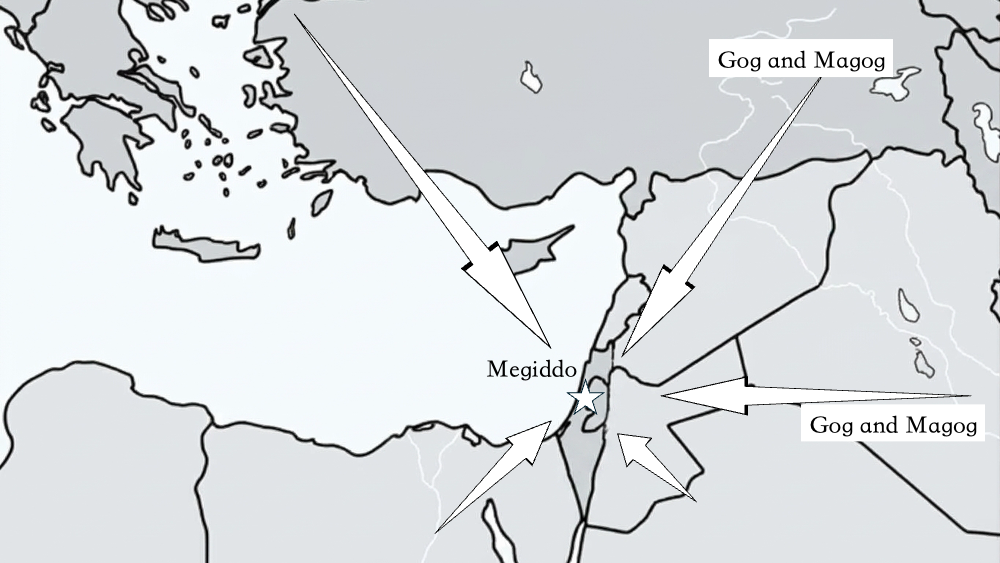
\includegraphics[
    width=1\textwidth,
    trim=0 0 0 0,
    clip]{images/Armageddon_english.png}
\end{figure}

\begin{ScriptureBox}

\item[20:8] and will go out to deceive the nations in the four corners of the earth---Gog and Magog---and to gather them for battle. In number they are like the sand on the seashore.

\item[20:9] They marched across the breadth of the earth and surrounded the camp of God's people, the city he loves. But fire came down from heaven and devoured them.

\item[20:10] And the devil, who deceived them, was thrown into the lake of burning sulfur, where the beast and the false prophet had been thrown. They will be tormented day and night for ever and ever.

\end{ScriptureBox}

Although Gog and Magog\index{Gog and Magog} appear in only one verse of Revelation 20, these names have a much longer history in biblical prophecy. They already appear in Ezekiel\index{Ezekiel} 38--39, where Gog comes from the far north and leads a great coalition of nations against God's people.

In Revelation, however, Gog and Magog\index{Gog and Magog} are portrayed as nations gathered from the four corners of the earth. They surround the camp of the saints and the beloved city, only to be consumed when fire comes down from heaven (Revelation 20:9).

John is drawing upon Ezekiel's prophetic imagery, but he presents it from a somewhat different perspective. This may be described as an eschatological reconfiguration: Revelation does not merely repeat the Old Testament's visions of the end. It brings together familiar prophetic images and places them within the unfolding story of Christ's redemption\index{redemption} and God's final judgment, allowing those images to serve a renewed purpose.

One detail is especially worth noting. In Revelation 19, Christ defeats the hostile forces gathered for the battle associated with Armageddon\index{Armageddon}. In Revelation 20, the vision of Gog and Magog\index{Gog and Magog} portrays the destruction of the forces of evil once more, now from a different angle.

Christians differ over whether these visions describe distinct events in chronological succession or portray the same ultimate conflict from different perspectives. Yet both visions declare the same truth: evil may gather its forces in a final, desperate rebellion, but its defeat is certain.

The nations may rise in overwhelming numbers. Their armies may surround the beloved city. For a moment, their power may seem irresistible. Yet the outcome does not depend on the strength of God's people or the size of their enemies. The final word belongs to God. The fire descends from heaven, the rebellion ends, and Satan\index{Satan}'s power is brought to its everlasting judgment.

\section{The Final Judgment: Before the Great White Throne}\index{great white throne}\index{judgment}

\begin{ScriptureBox}

\item[20:11] Then I saw a great white throne and him who was seated on it. The earth and the heavens fled from his presence, and there was no place for them.

\item[20:12] And I saw the dead, great and small, standing before the throne, and books were opened. Another book was opened, which is the book of life. The dead were judged according to what they had done as recorded in the books.

\item[20:13] The sea gave up the dead that were in it, and death and Hades gave up the dead that were in them, and each person was judged according to what they had done.

\item[20:14] Then death and Hades were thrown into the lake of fire. The lake of fire is the second death.

\item[20:15] Anyone whose name was not found written in the book of life was thrown into the lake of fire.

\end{ScriptureBox}

John now sees a great white throne\index{great white throne}. Before the One seated upon it, heaven and earth flee away, and no place remains for them. The present order of creation is passing away, and God's final judgment has arrived.

The dead stand before the throne\index{throne of God}, great and small alike. The books are opened, and another book is opened as well: the book of life\index{book of life}. All are judged according to what is recorded in the books, according to what they have done.

No one can evade this final reckoning. No earthly distinction can shield anyone from the gaze of the One who judges. Rank and reputation, wealth and poverty, greatness and obscurity—all fall away before the throne of God. Every life must answer to Him.

The vision is solemn, and we should not soften its warning. Yet it also brings the whole story of Revelation into sharp focus. The evil that once seemed unconquerable has been overthrown. Satan\index{Satan} has been cast into the lake of fire\index{lake of fire}. Even Death and Hades\index{Hades} are abolished. The enemies that have tormented God's creation will not endure forever.

The final division is absolute: life or the second death\index{second death}. Those whose names are written in the book of life\index{book of life} belong to God; those whose names are not found there face the judgment of the lake of fire\index{lake of fire}.

This vision calls us to examine our lives honestly, but it also directs our attention beyond our own deeds to the God before whom every person must stand. The book of life\index{book of life} reminds us that our ultimate hope cannot rest in worldly achievement or self-assurance. It rests in God's saving grace\index{grace} and in the victory of Jesus Christ, the Lamb who was slain\index{Lamb, the!slain} and who reigns forever.

\begin{figure}[htbp]
    \centering
    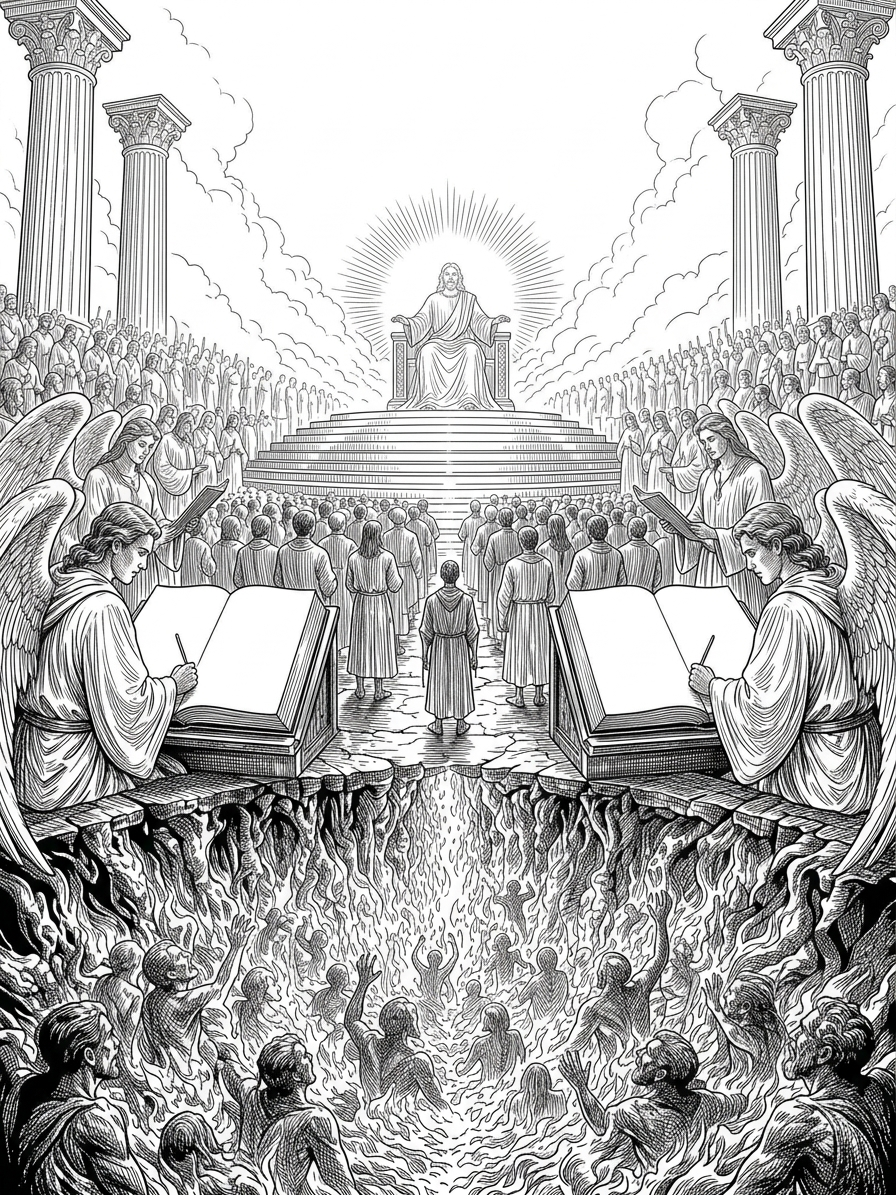
\includegraphics[
    width=1\textwidth,
    trim=0 0 0 0,
    clip]{images/white_throne_judgement.jpg}
\end{figure}

\section*{Discussion Questions}

\begin{enumerate}

    \item Read Revelation 20:11--15, the vision of the great white throne. What is your strongest response to this passage: a sense of warning, reverence, comfort, or hope? Why?

    \item If you are confident that Christ will ultimately triumph, that Satan will be defeated, and that death itself will be abolished, how might this confidence change the way you live today? In your family, at work, in the church, or amid suffering, what truth do you most need to hold fast to?

\end{enumerate}
\chapter{Brought into Glory by Grace (21:1--22:21)}\index{glory}\index{grace}

At last, we have arrived at the new heaven and the new earth. Someone might ask, ``I have not even finished my journey through this life. Why should I already be longing for the new heaven and the new earth of eternity?''

Let me offer a simple illustration.

Imagine that you are preparing to move into a spacious, beautiful new home. Everything has been made ready, and you know that one day you will live there. Yet the children and teenagers in your household are reluctant to leave the house. They might say, ``Isn't it good enough to live here? Why do we have to move?'' Would you respond to them that, if they feel that way, you will simply abandon the move? Of course not. Instead, you would take them to see the new home. You would help them imagine the life that awaits them. 

Hebrews 11:16 reminds us that God's people are strangers and pilgrims on the earth, longing for a better place, a heavenly one. God has prepared a city for them. And when the Lord Jesus was preparing to depart from His disciples, He told them that He was going to prepare a place for them (John 14:2). Our hope in the new heaven and the new earth rests on this same promise.

We do not long for the life to come because we despise the life we have now. We come to know Christ, learn to love others, and serve our Lord. Yet we know that even these precious gifts are not the end of the story.

God has prepared a better place for His people: a glorious\index{glory} dwelling in which He will renew heaven and earth and live among them forever.

Therefore, Christians can cherish the present while looking forward to that day. We can faithfully complete the journey set before us while lifting our eyes toward the glory that lies ahead.

\begin{figure}[h]
    \centering
    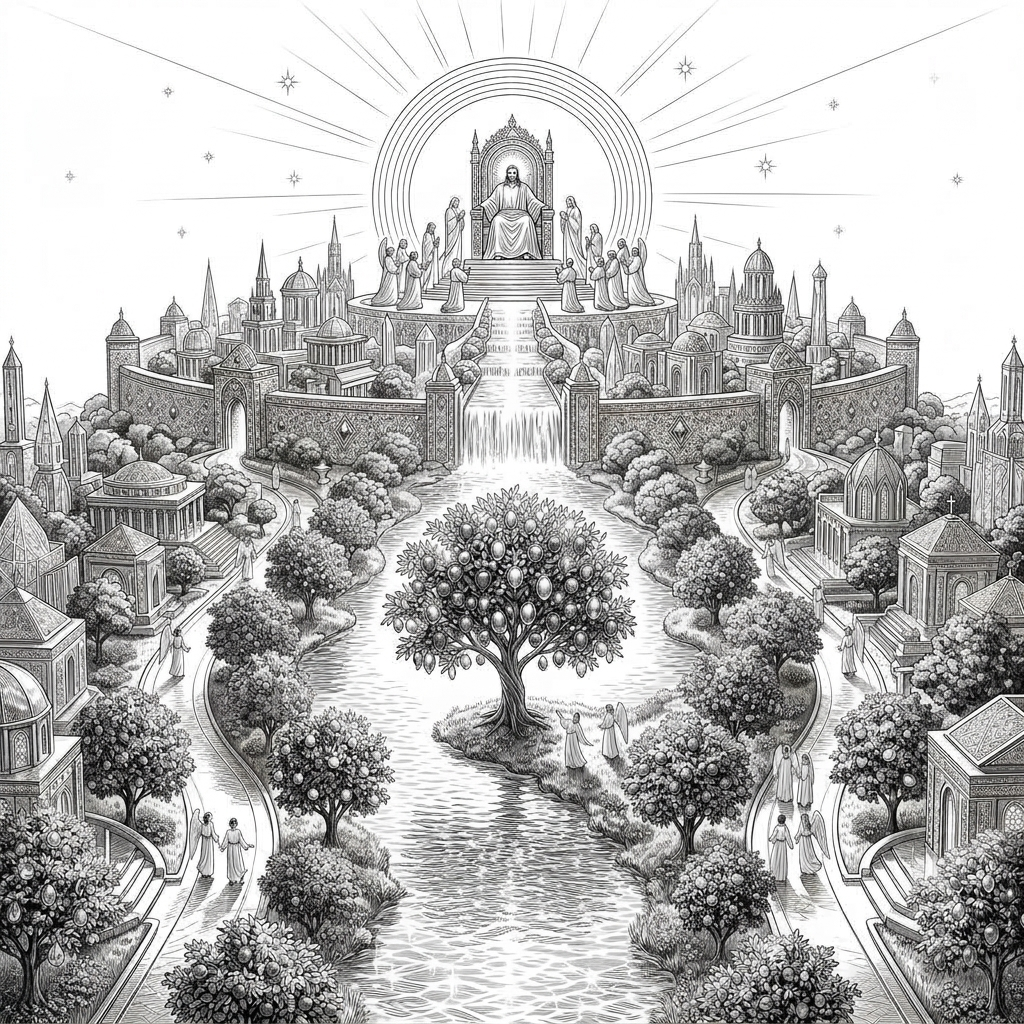
\includegraphics[
    width=1\textwidth,
    trim=0 0 0 0,
    clip]{images/tree_of_life.jpg}
\end{figure}

\section{All Things Made New: God Dwelling with His People}

\begin{ScriptureBox}

\item[21:1] Then I saw ``a new heaven and a new earth,'' for the first heaven and the first earth had passed away, and there was no longer any sea.
% NIV footnote for 21:1: ``a new heaven and a new earth'' --- Isaiah 65:17

\item[21:2] I saw the Holy City, the new Jerusalem, coming down out of heaven from God, prepared as a bride beautifully dressed for her husband.

\item[21:3] And I heard a loud voice from the throne saying, ``Look! God's dwelling place is now among the people, and he will dwell with them. They will be his people, and God himself will be with them and be their God.

\item[21:4] `He will wipe every tear from their eyes. There will be no more death' or mourning or crying or pain, for the old order of things has passed away.''
% NIV footnote for 21:4: ``no more death'' --- Isaiah 25:8
% CHECK NIV: footnote references for 21:1 and 21:4 quoted from memory;
%   verify against Bible Gateway.

\item[21:5] He who was seated on the throne said, ``I am making everything new!'' Then he said, ``Write this down, for these words are trustworthy and true.''

\item[21:6] He said to me: ``It is done. I am the Alpha and the Omega, the Beginning and the End. To the thirsty I will give water without cost from the spring of the water of life.

\item[21:7] Those who are victorious will inherit all this, and I will be their God and they will be my children.

\item[21:8] But the cowardly, the unbelieving, the vile, the murderers, the sexually immoral, those who practice magic arts, the idolaters and all liars---they will be consigned to the fiery lake of burning sulfur. This is the second death.''

\end{ScriptureBox}

One word stands out as we read about the new heaven and the new earth and the New Jerusalem\index{New Jerusalem}: \textbf{new}. But what does this newness mean?

If we were to enter the new heaven and the new earth still as the people we once were, with our old lives, our old dispositions, and our old sins, would we not be out of place in such a holy dwelling? God is not merely renewing the heavens and the earth. He is also renewing His people, preparing them to live with Him forever.

Paul writes that although our outward nature is wasting away, our inward nature is being renewed day by day (2 Corinthians 4:16). Our renewal does not begin only when we enter the new heaven and the new earth. It has already begun in Christ. Today, God is at work transforming us; on that day, He will bring His work to completion.

Consider the robber who was crucified beside Jesus. He had lived a sinful life and was dying under the sentence of his own wrongdoing. Yet, in his final hours, he recognized something extraordinary in the Man who hung beside him. He acknowledged his own guilt and asked Jesus to remember him.

Jesus answered him with the promise of paradise (Luke 23:43).

The man had no time to rebuild his life, no opportunity to establish a record of good works or prove through years of conduct that he had changed. Yet his heart turned toward Christ. The man who had lived in sin now looked to Jesus and entrusted himself to Him.

This is the transforming power of grace\index{grace}.

The new heaven and the new earth will not be inhabited by people who remain devoted to sin. They will be God's redeemed\index{redemption} people, whom He has already begun to renew in Christ, whom He continues to transform in this life, and whom He will one day glorify completely.

Who is the One who makes all things new?

He declares, ``It is done.'' He is the Alpha and the Omega\index{Alpha and Omega}, the Beginning and the End. He freely gives the water of life\index{water of life} to the thirsty.

We are reminded of Jesus' encounter with the Samaritan woman at Jacob's well. There, He promised that whoever drinks the water He gives will never thirst again, for His gift becomes a spring welling up to eternal life (John 4:14).

The One who promises to renew all things is the same One who offers us living water today. The life of the coming age is not a distant hope detached from our present walk with Him. 

\section{The Bride Is the New Jerusalem}\index{New Jerusalem}\index{bride of the Lamb}

\begin{ScriptureBox}

\item[21:9] One of the seven angels who had the seven bowls full of the seven last plagues came and said to me, ``Come, I will show you the bride, the wife of the Lamb.''

\item[21:10] And he carried me away in the Spirit to a mountain great and high, and showed me the Holy City, Jerusalem, coming down out of heaven from God.

\item[21:11] It shone with the glory of God, and its brilliance was like that of a very precious jewel, like a jasper, clear as crystal.

\item[21:12] It had a great, high wall with twelve gates, and with twelve angels at the gates. On the gates were written the names of the twelve tribes of Israel.

\item[21:13] There were three gates on the east, three on the north, three on the south and three on the west.

\item[21:14] The wall of the city had twelve foundations, and on them were the names of the twelve apostles of the Lamb.

\item[21:15] The angel who talked with me had a measuring rod of gold to measure the city, its gates and its walls.

\item[21:16] The city was laid out like a square, as long as it was wide. He measured the city with the rod and found it to be 12,000 stadia in length, and as wide and high as it is long.
% NIV footnote for 21:16: ``12,000 stadia'' --- That is, about 1,400 miles
%   or about 2,200 kilometers

\item[21:17] The angel measured the wall using human measurement, and it was 144 cubits thick.
% NIV footnotes for 21:17:
%   ``144 cubits'' --- That is, about 200 feet or about 65 meters
%   ``thick'' --- Or high

\item[21:18] The wall was made of jasper, and the city of pure gold, as pure as glass.

\item[21:19] The foundations of the city walls were decorated with every kind of precious stone. The first foundation was jasper, the second sapphire, the third agate, the fourth emerald,

\item[21:20] the fifth onyx, the sixth ruby, the seventh chrysolite, the eighth beryl, the ninth topaz, the tenth turquoise, the eleventh jacinth, and the twelfth amethyst.
% NIV footnote for 21:20: end of verse --- The precise identification of
%   some of these precious stones is uncertain.
% CHECK NIV: footnote wording for 21:16--20 quoted from memory;
%   verify against Bible Gateway.

\item[21:21] The twelve gates were twelve pearls, each gate made of a single pearl. The great street of the city was of gold, as pure as transparent glass.

\end{ScriptureBox}

The holy city\index{holy city} descends from heaven, radiant with splendor and filled with the glory of God. John looks upon it carefully, taking in its gates, its foundations, and its extraordinary beauty.

There are three gates on each side of the city, and the names of the twelve tribes\index{twelve tribes of Israel} of Israel\index{Israel} are written upon them. The city wall rests on twelve foundations, bearing the names of the Lamb\index{Lamb, the}'s twelve apostles.

This vision calls to mind Jesus' words to Peter: He would build His church upon the rock, and the gates of Hades\index{Hades} would not overcome\index{overcomers} it (Matthew 16:18).

The New Jerusalem\index{New Jerusalem} has twelve foundations associated with the twelve apostles of the New Testament and twelve gates bearing the names of the twelve tribes\index{twelve tribes of Israel} of Israel. Together, these features point to the unity and completeness of God's redemptive purpose. The people of God in the Old Testament and the redeemed community gathered through Christ are brought together in one glorious dwelling.

This does not erase the distinction between Israel and the Church in every theological discussion. Rather, the imagery shows that God's saving purpose reaches its fulfillment in the city He has prepared for His people, a city whose foundations and gates bear witness to the unfolding story of redemption.

For Christians, this vision also affirms that our faith is firmly grounded. As Ephesians 2:20 teaches, God's household is built on the foundation of the apostles and prophets, with Christ Jesus Himself as the chief cornerstone.

The city is given precise measurements, suggesting perfection, holiness, and completeness. It is shaped like a perfect cube, with its length, width, and height equal. Its dimensions are twelve thousand \textit{stadia.}
In modern measurements, twelve thousand stadia is approximately 1,400 miles, or about 2,250 kilometers.

Imagine, then, a city whose length, width, and height each extend for roughly 1,400 miles. Picture an immense cube, radiant with the glory of God, rising far beyond the scale of anything we have known.

\begin{figure}[htbp]
    \centering
    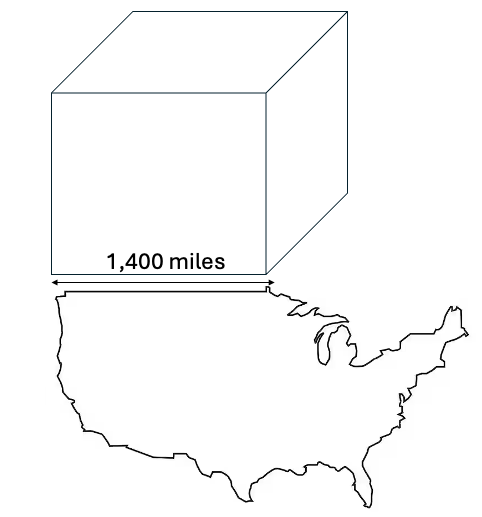
\includegraphics[
    width=0.6\textwidth,
    trim=0 0 0 0,
    clip]{images/new_jesusalem_US.png}
\end{figure}


What a magnificent city!

And Revelation 7:9 has already shown us an innumerable multitude standing before the throne\index{throne of God} and before the Lamb, drawn from every nation, tribe, people, and language.

The vision invites us to imagine the vastness of the redeemed community dwelling in God's presence, no longer divided by hostility or separated from Him by sin and death. The dimensions of the city are not given to satisfy our curiosity alone. They direct our attention toward the greatness of the God who prepares such a dwelling for His people.

This comparison is only a small aid to our imagination. The glory of the New Jerusalem\index{New Jerusalem} exceeds anything we can fully comprehend. As Paul reminds us, God has prepared things for those who love Him that human eyes have not seen, ears have not heard, and hearts have not conceived (1 Corinthians 2:9).


\section{God Himself Is the Temple of the City}\index{temple}

\begin{ScriptureBox}

\item[21:22] I did not see a temple in the city, because the Lord God Almighty and the Lamb are its temple.

\item[21:23] The city does not need the sun or the moon to shine on it, for the glory of God gives it light, and the Lamb is its lamp.

\item[21:24] The nations will walk by its light, and the kings of the earth will bring their splendor into it.

\item[21:25] On no day will its gates ever be shut, for there will be no night there.

\item[21:26] The glory and honor of the nations will be brought into it.

\item[21:27] Nothing impure will ever enter it, nor will anyone who does what is shameful or deceitful, but only those whose names are written in the Lamb's book of life.

\end{ScriptureBox}

Those who dwell in the city are people who have been saved by grace. Their names are written in the Lamb's book of life\index{book of life}. They are the work of God's grace.

In Christ, God has chosen, called, forgiven, and preserved His people, bringing them at last into the eternal city He has prepared. Their presence there is not the reward of human achievement, but the fulfillment of God's saving purpose.

The redeemed share a common identity: they belong to the Lamb who gave Himself for them. Yet the vision also preserves the richness of the nations. The glory of the city is not portrayed as the erasure of every distinction among peoples. Rather, the nations bring their splendor into the light of God's presence.

Differences that once became occasions for division no longer stand in opposition to the worship\index{worship} of God. The redeemed gather in unity, and the diversity of the nations becomes part of the rich beauty of their common praise.

What a beautiful vision of the people of God, gathered at last in the light of His glory!

And at the heart of it all stands a remarkable truth: there is no temple\index{temple} in the city. God's people no longer approach Him through an earthly sanctuary, for the Lord God Almighty and the Lamb are themselves the temple. The presence for which the people of God have longed throughout the ages is now their everlasting home.

\begin{ReaderQuestion}
From the Garden of Eden, through the tabernacle and the temple, to the incarnation of Christ and finally the new heaven and the new earth, how do you see God's promise to dwell with His people unfolding throughout the Bible?
\end{ReaderQuestion}

\section{The River of Life and the Tree of Life}\index{water of life}\index{tree of life}

\begin{ScriptureBox}

\item[22:1] Then the angel showed me the river of the water of life, as clear as crystal, flowing from the throne of God and of the Lamb

\item[22:2] down the middle of the great street of the city. On each side of the river stood the tree of life, bearing twelve crops of fruit, yielding its fruit every month. And the leaves of the tree are for the healing of the nations.

\item[22:3] No longer will there be any curse. The throne of God and of the Lamb will be in the city, and his servants will serve him.

\item[22:4] They will see his face, and his name will be on their foreheads.

\item[22:5] There will be no more night. They will not need the light of a lamp or the light of the sun, for the Lord God will give them light. And they will reign for ever and ever.

\end{ScriptureBox}

The opening verses of Revelation 22 bring us back to the Garden of Eden\index{Eden} in Genesis. There, we encountered the tree of life\index{tree of life} and the river that watered the garden. Here, the river of the water of life\index{water of life} flows from the throne of God and of the Lamb.

Human life depends upon God and finds its fullest joy in Him. Life is His gift, and the blessings of the new creation flow from His presence. The tree of life\index{tree of life} bears fruit every month, continually sustaining the life and flourishing of God's people.

John also tells us that the leaves of the tree are for the healing of the nations. This does not necessarily imply that disease will persist in the new creation. In the context of a world where death, pain, and the curse have been abolished, the imagery points toward the complete restoration and enduring well-being of the nations. The tree represents the fullness of life God provides, not a continuing struggle against illness.\footnote{See John MacArthur's discussion of Revelation 22 in his commentary on Revelation (2007).}

Verse 3 declares that there will no longer be any curse. These words take us back to Genesis 3, where sin entered the world and the curse followed. Now, in Revelation 22, redemption has reached its fulfillment, and the curse is removed forever.

Table \ref{tab:genesis3-rev21-22} shows the comparison between the beginning and the end of the biblical story.

{
\renewcommand{\arraystretch}{1}
\small
\begin{longtable}{>{\raggedright\arraybackslash}p{0.45\textwidth} >{\raggedright\arraybackslash}p{0.45\textwidth}}
\caption{Paradise lost and paradise restored: Genesis 3 and Revelation 21--22}
\label{tab:genesis3-rev21-22} \\
\hline
\textbf{Genesis 3} & \textbf{Revelation 21--22} \\
\hline
\endfirsthead

\multicolumn{2}{l}{\small\itshape Table~\thetable\ (continued)} \\
\hline
\textbf{Genesis 3} & \textbf{Revelation 21--22} \\
\hline
\endhead

\hline
\endfoot

\hline
\endlastfoot

Sin enters the world & All things are made new \\
The curse falls upon creation & There is no more curse \\
Humanity is driven from Eden & God's people enter the holy city \\
Access to the tree of life is lost & God's people receive the blessings of the tree of life \\
Humanity is separated from God & God dwells with His people \\
Death enters the world & Death is no more \\
The serpent deceives humanity & Satan is utterly defeated \\
Humanity loses the joy of God's presence & God's servants see His face \\
\end{longtable}
}


The Bible's story begins in a garden and reaches its fulfillment in a city. What was lost through sin is restored through the saving work of God. Yet the final vision is more than a return to Eden\index{Eden}. The redeemed dwell in the presence of God and the Lamb, their fellowship with Him no longer threatened by sin, suffering, or death.

The story that began with the tragedy of human rebellion ends with the triumph of divine grace.

\section{Do Not Seal Up the Words of This Book}

Now the book of Revelation speaks directly to us. The angel declares that these words are trustworthy and true. 

\begin{ScriptureBox}

\item[22:6] The angel said to me, ``These words are trustworthy and true. The Lord, the God who inspires the prophets, sent his angel to show his servants the things that must soon take place.''

\item[22:7] ``Look, I am coming soon! Blessed is the one who keeps the words of the prophecy written in this scroll.''

\item[22:8] I, John, am the one who heard and saw these things. And when I had heard and seen them, I fell down to worship at the feet of the angel who had been showing them to me.

\item[22:9] But he said to me, ``Don't do that! I am a fellow servant with you and with your fellow prophets and with all who keep the words of this scroll. Worship God!''

\item[22:10] Then he told me, ``Do not seal up the words of the prophecy of this scroll, because the time is near.

\item[22:11] Let the one who does wrong continue to do wrong; let the vile person continue to be vile; let the one who does right continue to do right; and let the holy person continue to be holy.''

\item[22:12] ``Look, I am coming soon! My reward is with me, and I will give to each person according to what they have done.

\item[22:13] I am the Alpha and the Omega, the First and the Last, the Beginning and the End.

\item[22:14] ``Blessed are those who wash their robes, that they may have the right to the tree of life and may go through the gates into the city.

\item[22:15] Outside are the dogs, those who practice magic arts, the sexually immoral, the murderers, the idolaters and everyone who loves and practices falsehood.

\end{ScriptureBox}

They were not given merely to satisfy curiosity about the future. They were given to God's people to be read, heard, kept, and obeyed.


Once again, we hear Jesus declare who He is:

``I am the Alpha and the Omega\index{Alpha and Omega}, the First and the Last, the Beginning and the End.''

Alpha is the first letter of the Greek alphabet, and Omega is the last. The whole course of history lies under His sovereign rule. From creation to the new heaven and the new earth, from the cross to glory, nothing lies beyond His authority or outside His redemptive purpose.

We also encounter a solemn statement: the one who does wrong will continue to do wrong, and the one who is holy will continue to be holy. These words should not be taken as permission to remain in sin. Rather, they confront us with the seriousness of the paths we choose and the loyalties we cultivate.

As history approaches its appointed end, the true character of human lives will be revealed. The fruit of a person's life will bear witness to the direction of the heart and to the allegiance that has shaped it. The final judgment\index{judgment} will expose what has been hidden, and no outward appearance will conceal the truth.

This warning calls us to examine ourselves before God. It also reminds us that the present is a time of grace, a time to turn from sin, trust in Christ, and walk in the holiness He gives His people.

The One who is coming is also the One who sees us now. His promise is certain, His judgment is righteous, and His invitation remains open.

\section{The Final Gospel Invitation: Let the Thirsty Come}

\begin{ScriptureBox}

\item[22:16] ``I, Jesus, have sent my angel to give you this testimony for the churches. I am the Root and the Offspring of David, and the bright Morning Star.''
% NIV footnote for 22:16 (omitted; add as \footnote if wanted):
%   ``you'' --- The Greek is plural.
% CHECK NIV: footnote wording quoted from memory; verify against Bible Gateway.

\item[22:17] The Spirit and the bride say, ``Come!'' And let the one who hears say, ``Come!'' Let the one who is thirsty come; and let the one who wishes take the free gift of the water of life.

\end{ScriptureBox}

At the end of Revelation, we hear one final invitation, addressed to everyone who reads these words and still thirsts for life:

``Let the thirsty come; and let the one who wishes take the free gift of the water of life\index{water of life}'' (Revelation 22:17, NIV).

What a beautiful gospel invitation!

It brings us back to Jesus' conversation with the Samaritan woman at the well. He promised that whoever drinks the water He gives will never thirst again, for that water becomes a spring welling up to eternal life (John 4:14).

The invitation is not a call to earn eternal life through human achievement. It is an invitation to receive what God freely gives. The thirsty are not told to make themselves worthy before approaching Him. They are invited to come.

God's purpose is to bring people into the glory of eternal life, where they will drink deeply of the life He provides and dwell in His presence forever.

The gospel invitation also reveals the heart of the One who calls us. The God who will judge the world is the same God who offers the water of life\index{water of life} freely. The Lamb who will bring history to its appointed end is the Lamb who gave His life to redeem His people.

The final invitation of Scripture therefore remains open to all who will come to Christ in faith. The thirsty may come. The weary may come. Those who know their need may come. The gift is not purchased by merit; it is received through grace.

\begin{ReaderQuestion}
If you were explaining Revelation 22:17 to someone who does not yet believe in Christ but feels a deep thirst in life, how would you describe the invitation? How does this verse show that the gospel is a gift of grace rather than something we purchase through good deeds or personal merit?
\end{ReaderQuestion}

\section{``Come, Lord Jesus''}

\begin{ScriptureBox}

\item[22:18] I warn everyone who hears the words of the prophecy of this scroll: If anyone adds anything to them, God will add to that person the plagues described in this scroll.

\item[22:19] And if anyone takes words away from this scroll of prophecy, God will take away from that person any share in the tree of life and in the Holy City, which are described in this scroll.

\item[22:20] He who testifies to these things says, ``Yes, I am coming soon.''\\
Amen. Come, Lord Jesus.

\item[22:21] The grace of the Lord Jesus be with God's people. Amen.

\end{ScriptureBox}

Revelation closes with two voices answering one another. The Lord Jesus declares, ``I am coming soon,'' and the Church responds, ``Amen. Come, Lord Jesus.''

Their exchange reminds us of the longing expressed in the Song of Songs, where the beloved longs for the arrival of the one she loves. The bride\index{bride of the Lamb}'s deepest desire is not merely to enjoy a wedding feast, but to be with her beloved.

So it is with the Church. Our hope is not simply that suffering will end, that injustice will be put right, or that the world will finally be made whole. These promises are precious, but at the heart of our hope stands a Person: Jesus Christ, the Lamb who loved us, gave Himself for us, and rose from the dead.

We long for Him to come.

His promise, ``I am coming soon,'' sustains us as we wait. It gives us courage in suffering, steadiness in uncertainty, and strength to remain faithful when the road grows difficult. We do not know every detail of the journey ahead, but we know the One who holds its end in His hands.

The final words of Revelation are therefore not merely a prediction about the future. They are the confession of a people whose hearts have been captured by grace. We have been called by Christ, redeemed by His blood, renewed by His Spirit, and promised a place in the city where God will dwell with His people forever.

And so we wait—not with empty hands or hopeless hearts, but with our eyes fixed on the returning King.

``Amen. Come, Lord Jesus.''

\begin{ReaderQuestion}
What does ``Come, Lord Jesus'' mean to you? How can this longing become more than a hope for the future and shape your prayers and choices today? In your work, family, suffering, service, and uncertainty about the future, how might the promise of Christ's return change the way you live?
\end{ReaderQuestion}

\appendix
\setcounter{figure}{0} 
\renewcommand{\thesection}{Appendix~\Alph{chapter}.\arabic{section}}
\refstepcounter{chapter} 
\chapter*{Frequently Asked Questions} 
\markboth{Appendix~\thechapter\quad Frequently Asked Questions}%
         {Appendix~\thechapter\quad Frequently Asked Questions}
\addcontentsline{toc}{chapter} {\protect\numberline{Appendix}}
\addcontentsline{toc}{chapter} {\protect\numberline{\thechapter} Frequently Asked Questions}

\def\theHfigure{appendix.\arabic{figure}}

\noindent \textbf{Q1. When Someone You Love Passed Away, and You Cannot Find Your Way Through the Grief}

You must miss deeply the brother or sister with whom you shared so much of life's journey. And perhaps your longing for our heavenly home has grown stronger than ever. I believe the Lord knows the ache of your heart and understands how difficult this journey of separation can be. Yet the Lord has chosen to leave you here on earth for a time. You have not been left behind to bear your sorrow alone. You are caught up in grace, and one day will be brought into His glory.

One day, we will be with Christ, the Lord of heaven and earth. Our greatest hope is to dwell with Him forever and behold His glory face to face. 

Dear sister, as you walk through the days on earth, may you continue to fix your eyes on Christ. He is not only your refuge in this life but also your hope for eternity. May the Lord Himself sustain you, so that day by day you may experience His presence and grace.

The Lord has promised that He will wipe away our tears.
Ecclesiastes 3:1, 4 reminds us that there is a time for everything: a time to weep and a time to laugh, a time to mourn and a time to dance.

If you begin to experience joy again, it does not mean that you love your husband any less. If you travel or attend a gathering, it does not mean that you have forgotten him. You may continue to cherish the memories of the life you shared, even as you slowly learn to live with his absence. 

\vspace{0.3cm}

\noindent \textbf{Q2. At the Resurrection, People Will Neither Marry nor Be Given in Marriage; They Will Be Like the Angels in Heaven (Matthew 22:30)}

I can only imagine the scene in Revelation 7:9--10:

\begin{quote}
``After this I looked, and there before me was a great multitude that no one could count, from every nation, tribe, people and language, standing before the throne and before the Lamb. They were wearing white robes and were holding palm branches in their hands. And they cried out in a loud voice:

`Salvation belongs to our God, who sits on the throne, and to the Lamb.' ''
\end{quote}

Perhaps, amid that vast multitude, you will catch sight of your husband.

Yet the one standing before you will no longer appear just as you knew him on earth. Clothed in white, his eyes shining with joy, he will be praising the greatness of salvation. With his whole being, he will worship the Lord who redeemed him. His life will be centered entirely on Christ. His deepest desire will be to draw near to the Lord, to know Him more fully, to praise Him, and to walk with Him throughout eternity.

You may discover that the man you meet there is far more glorious than the man you knew in this life.

You knew him well. You knew how he devoted himself in his work. You knew that he used to drink a cup of coffee before leaving for work each morning. You were familiar with his joys and sorrows, his laughter and frustration. You walked beside him through life's rises and falls. Yet on that day, he will no longer be constrained by the weakness, toil, and sorrow of this present life. He will have received an imperishable, glorified body (1 Corinthians 15:42--44).

But you, too, will have changed.

You will be standing among that same multitude from every nation, tribe, people, and language, clothed in white and holding a palm branch in your hand. Together, you will offer praise to God, who sits on the throne, and to the Lamb. Before you will be the Savior who knows you more completely than anyone else. You will love and worship Him and walk with Him forever.

As 1 Corinthians 13:12 says, ``For now we see only a reflection as in a mirror; then we shall see face to face.'' Our knowledge of the Lord is limited in this life, but one day we will know Him more fully. 

\vspace{0.3cm}


\noindent \textbf{Q3. If I Am in Heaven One Day, but the Family Members I Love Are Not There, Will I Still Be Able to Rejoice?}

When we think of our parents, spouse, children, or siblings, it is difficult to imagine how we could rejoice in heaven if those we love are not there. Will we remember them? If we do, how can we be free from sorrow?

Scripture does not fully explain how the redeemed will remember or understand the final destiny of loved ones who are not saved. We must therefore approach this question with humility, trusting what God has revealed without speculating beyond His Word.

\textbf{First}, will we remember those we love?

We know that after His resurrection, Jesus remained the same Lord who had been crucified and then raised from the dead. In a similar way, God will transform our lowly bodies so that they will be like His glorious body (Philippians 3:21). Yet Scripture does not explicitly tell us how our memories of those who were not saved will remain, or how we will understand those memories in eternity. We should be careful not to claim more than God has revealed.

\textbf{Second}, how can we rejoice if someone we love is not in heaven?
Revelation 21:4 promises:

\begin{quote}
``He will wipe every tear from their eyes. There will be no more death or mourning or crying or pain, for the old order of things has passed away.''
\end{quote}

God promises that sorrow and pain will be no more. Although Scripture does not explain how this promise relates to our memories of those who are lost, we can trust that God's promise will never fail. Revelation 16:7 declares, ``Yes, Lord God Almighty, true and just are your judgments.'' We can trust both His perfect justice and His unfailing goodness, even when we do not understand how He will resolve this mystery.

\textbf{Third}, God's holiness and compassion do not contradict one another.
Jesus knew the reality of sin and judgment, yet He grieved over Jerusalem (Matthew 23:37). His example reminds us that compassion for sinners is not incompatible with God's holiness and justice.

How, then, should we respond today? Paul expressed ``great sorrow and unceasing anguish'' for his fellow Israelites (Romans 9:2–3). His example reminds us that grieving over the spiritual condition of those we love is not evidence of weak faith.

We should continue to pray for our loved ones, share the gospel, and trust them to God. We do not know every person's final destiny, nor can we fully understand the mysteries of eternity. But we know the character of the God who holds eternity in His hands. He is perfectly just, unfailingly good, and faithful to every promise He has made.

%\appendix
\refstepcounter{chapter} 
\chapter*{Major Views of the End Times} 
\markboth{Appendix~\thechapter\quad Major Views of the End Times}%
         {Appendix~\thechapter\quad Major Views of the End Times}
%\addcontentsline{toc}{chapter} {\protect\numberline{Appendix~\thechapter} Major Views of the End Times}
\addcontentsline{toc}{chapter} {\protect\numberline{\thechapter} Major Views of the End Times}


The Book of Revelation is commonly interpreted through four major approaches. The fundamental difference among them lies in how they understand the timing of the events Revelation describes: Have they already taken place, do they unfold throughout history, will they occur primarily in the future, or do they reveal spiritual realities that characterize every age?

\subsection*{Futurism}

The defining emphasis of Futurism is the \emph{future}. Futurists understand most of the visions beginning in chapter 4 as events that have yet to occur and that will unfold in sequence around the time of Christ's return. These events may include the appearance of a particular Antichrist, a period of great tribulation, and a thousand-year reign of Christ on earth following His return.

Compared with the other three approaches, Futurism generally places the greatest emphasis on reading Revelation's visions as a sequence of events yet to be fulfilled, often interpreting their descriptions in a more literal and chronological manner. Preterism sees the principal fulfillment in the past, Historicism traces the visions through successive periods of history, and Idealism emphasizes the spiritual realities they portray rather than identifying them with specific historical events.

One strength of Futurism is its serious attention to the fulfillment of prophecy. It reminds believers to remain watchful and to live in expectation of the Lord's return. Its principal challenge, however, is that it can make much of Revelation seem remote from the experience of its original readers in the first century.

\subsection*{Preterism}

The defining emphasis of Preterism is the \emph{past}, particularly the historical setting of John's own time in the first century. Preterists understand many of Revelation's prophecies as having already been fulfilled, especially in events associated with the Roman Empire's persecution of the church and the destruction of Jerusalem in A.D. 70.

Compared with the other three approaches, Preterism places the greatest emphasis on the historical background of Revelation and the circumstances of the early church. John explicitly states that the things revealed to him ``must soon take place'' (Revelation 1:1). From this perspective, the book was first given to suffering churches of the first century to strengthen their faith and assure them that God remained sovereign even amid persecution.

One strength of Preterism is that it closely connects Revelation with the people to whom it was originally written. It encourages readers to hear the message as those first believers might have heard it, in the midst of their own trials. Its principal challenge is explaining the full scope of the book's visions of final judgment and the renewal of all things. For this reason, most Preterists still affirm that Christ will return in the future, even though they understand many of Revelation's prophecies as already fulfilled.

\subsection*{Historicism}

The defining emphasis of Historicism is the unfolding of \emph{church history}. Historicists understand Revelation as a prophetic account of the course of history, extending from the apostolic age through successive historical periods to the return of Christ.

Unlike Preterism, which focuses primarily on the first century, or Futurism, which places most of the relevant events in the future, Historicism seeks to identify the visions with a succession of particular events, movements, and figures throughout history. For example, some historicist interpretations understand the seven churches as representing seven successive eras in the history of the church.

This approach was especially influential during the Reformation. One of its strengths is its emphasis on God's sovereignty over every stage of history. No empire, institution, or historical upheaval lies beyond His rule. Its principal challenge, however, is that interpreters have often disagreed about which events correspond to particular visions. Moreover, each generation can be tempted to regard its own age as the decisive culmination of the prophetic narrative. For these reasons, Historicism is less widely adopted among contemporary biblical scholars.

\subsection*{Idealism (the Symbolic Approach)}

The defining emphasis of Idealism is the enduring spiritual reality revealed through the visions. Rather than identifying each vision with a particular historical event, Idealists understand Revelation as portraying realities that characterize every age: the conflict between God and Satan, the suffering and faithful witness of the church, the deceptive allure of evil powers, and the ultimate victory of Christ.

Where the other three approaches tend to ask, ``When does this event take place?'' Idealism asks, ``What spiritual truth does this vision reveal?'' Its strength is that it brings Revelation's message directly to believers in every generation. The book speaks not only to Christians in the first century or to those living in the last days, but also to the church throughout its pilgrimage in this world.

Its principal challenge is the possibility of overlooking the book's concrete historical setting and the ways in which particular visions may have been fulfilled. For this reason, many interpreters combine Idealism with elements of other approaches. They first consider what a vision meant to its original readers, then examine how it speaks to the spiritual struggles of the church throughout history, and finally consider how it points toward Christ's return and the consummation of God's purposes.

\medskip

These four approaches need not be understood as entirely incompatible. A single vision may refer, in its original setting, to the Roman Empire; at the same time, it may reveal the spiritual conflict faced by the church throughout the ages and point forward to the final victory of Christ.

As we read Revelation, we need not lose sight of any of these horizons. We must listen carefully to the message given to the first-century churches, recognize the spiritual realities that continue to shape the church's life, and look forward with hope to the day when Christ will bring history to its appointed end. Above all, we must keep our eyes fixed on the One who reigns over history: the Lamb who was slain, who stands victorious, and who will lead His people into glory.
```
%\appendix 
\refstepcounter{chapter} 
\chapter*{How Long Is the Great Tribulation? The Seventy Sevens of Daniel}\index{Great Tribulation}\index{seventy sevens (Daniel 9)}\index{Daniel} 
\markboth{Appendix~\thechapter\quad How Long Is the Great Tribulation?}%
         {Appendix~\thechapter\quad How Long Is the Great Tribulation?}
%\addcontentsline{toc}{chapter} {\protect\numberline{Appendix~\thechapter} How Long Is the Great Tribulation? The Seventy Sevens of Daniel}
\addcontentsline{toc}{chapter} {\protect\numberline{\thechapter} How Long Is the Great Tribulation? The Seventy Sevens of Daniel}


\section*{A Seven-Year Great Tribulation}\index{Great Tribulation}

The following explanation represents the premillennialist\index{premillennialism} interpretation.

Daniel\index{Daniel} 9 is a key passage for understanding the events of the last days.

\begin{ScriptureBox}

\item[9:24] ``Seventy `sevens' are decreed for your people and your holy city to finish transgression, to put an end to sin, to atone for wickedness, to bring in everlasting righteousness, to seal up vision and prophecy and to anoint the Most Holy Place.''

\item[9:25] ``Know and understand this: From the time the word goes out to restore and rebuild Jerusalem until the Anointed One, the ruler, comes, there will be seven `sevens,' and sixty-two `sevens.' It will be rebuilt with streets and a trench, but in times of trouble.''

\item[9:26] ``After the sixty-two `sevens,' the Anointed One will be put to death and will have nothing. The people of the ruler who will come will destroy the city and the sanctuary. The end will come like a flood: War will continue until the end, and desolations have been decreed.''

\item[9:27] ``He will confirm a covenant with many for one `seven.' In the middle of the `seven' he will put an end to sacrifice and offering. And at the temple he will set up an abomination that causes desolation, until the end that is decreed is poured out on him.''

\end{ScriptureBox}

The angel told Daniel that seventy sevens\index{seventy sevens (Daniel 9)} had been decreed for his people and the holy city\index{holy city} of Jerusalem\index{Jerusalem}.

The underlying Hebrew expression refers to a unit of seven. In this context, it is commonly understood to mean seven years. Thus, seventy sevens\index{seventy sevens (Daniel 9)} amount to \(70 \times 7 = 490\) years.

In the traditional premillennialist\index{premillennialism} interpretation, the seventieth seven is a future seven-year period associated with the Great Tribulation\index{Great Tribulation}.

The first seven sevens (49 years) and the following sixty-two sevens (434 years) are generally understood within this interpretation as having already been fulfilled in history.

\begin{itemize}
\item \textbf{The seven sevens (49 years):} This period is commonly associated with the twentieth year of King Artaxerxes of Persia, around 445 B.C., when he authorized Nehemiah to return and rebuild Jerusalem\index{Jerusalem} (Nehemiah 2:1--8). The period begins with the command to restore and rebuild the city.

\item \textbf{The sixty-two sevens (434 years):} Together with the first seven sevens, this period makes sixty-nine sevens, or 483 years. If calculated using the 360-day year often employed in certain interpretations of biblical prophecy, 483 years amount to approximately 173,880 days. Some interpreters understand this calculation as pointing to the time when Jesus entered Jerusalem\index{Jerusalem} riding on a donkey and was welcomed as King. The words ``the Anointed One will be put to death and will have nothing'' are understood as referring to Christ's crucifixion.\footnote{The following statement, ``The people of the ruler who will come will destroy the city and the sanctuary,'' is commonly understood as referring to the Roman army's conquest of Jerusalem and destruction of the Temple in A.D. 70.}
\end{itemize}

\section*{The Great Tribulation as the Seventieth Seven}\index{Great Tribulation}

Readers may have noticed that, in this interpretation, Daniel\index{Daniel}'s seventy sevens\index{seventy sevens (Daniel 9)} do not follow one another without interruption. The first sixty-nine sevens belong to the past, while the seventieth seven remains in the future. A substantial interval lies between them.

One widely held explanation can be illustrated by the timeline shown in the figure below.

Imagine looking at a mountain range from a distance. Two peaks may appear to rise close together, almost as though they touch. Yet when you draw nearer, you discover a deep valley between them. The Old Testament prophets often saw future events in a similar way. They saw the mountain peaks: the Messiah\index{Messiah}'s suffering, the Messiah's glory\index{glory}, and the judgment\index{judgment} at the end of the age. These events appeared together in their prophetic vision, but the valley between them remained hidden from view. That valley represents the present age of the church.

This phenomenon is often called \emph{prophetic foreshortening}.\footnote{It is also known as ``prophetic telescoping'' or ``prophetic perspective.'' The mountain-peak illustration is one way of describing this feature of biblical prophecy.}

Figure \ref{fig:valley} shows the view. Period \ding{172} represents the 483 years associated with the fulfillment of the first sixty-nine sevens. Period \ding{173} represents the final seven, understood here as the future seven-year Great Tribulation\index{Great Tribulation}. Period \ding{174} represents the valley: the age of grace\index{grace} in which the church is gathered, a mystery not fully revealed to the Old Testament prophets.

{
\begin{figure}[htbp]
    \centering
    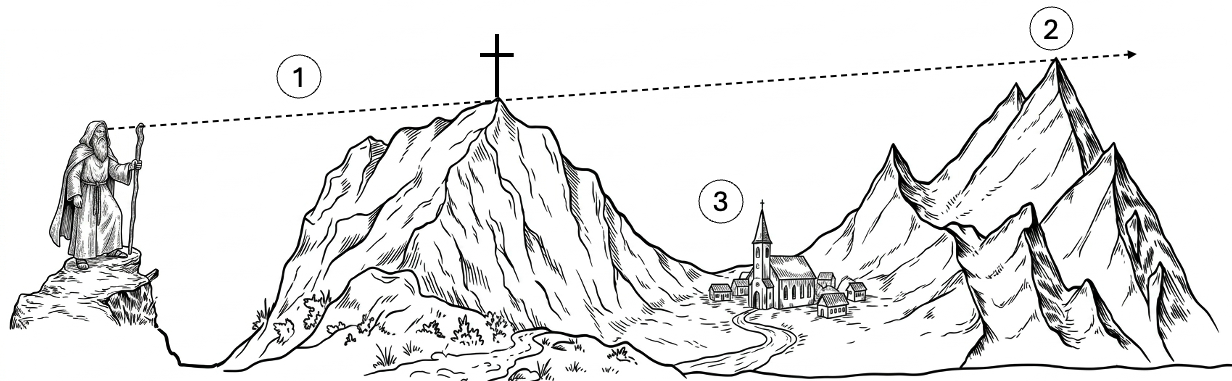
\includegraphics[
        width=1\textwidth,
        trim=0 0 0 0,
        clip]{images/mountain_peak_valley.png}
    \caption{Prophetic Foreshortening}
    \label{fig:valley}
\end{figure}
}

\normalsize

Why was the valley hidden from view?

Paul explains that the church was part of a \textbf{mystery} that had not been fully revealed in earlier generations. Ephesians 3:5 says that this mystery ``has now been revealed by the Spirit to God's holy apostles and prophets.'' Colossians 1:26 describes it as ``the mystery that has been kept hidden for ages and generations, but is now disclosed to the Lord's people.''%
\footnote{A particularly clear example appears when Jesus reads from Isaiah in the synagogue at Nazareth. He reads the words about proclaiming the year of the Lord's favor, then rolls up the scroll and declares, ``Today this scripture is fulfilled in your hearing'' (Luke 4:18--21, NIV). He does not continue to the next phrase in Isaiah 61:2, which speaks of the day of vengeance of our God. In Isaiah's prophecy, these two phrases stand close together. In their historical fulfillment, however, they are separated by at least two thousand years. This example shows that biblical prophecy can place events side by side in the prophetic vision even when a substantial interval separates their fulfillment. The interpretation of an interval between Daniel's sixty-ninth and seventieth sevens is therefore not without precedent in the broader pattern of biblical prophecy.}%
\footnote{Not all interpreters agree that an interval separates the sixty-ninth and seventieth sevens. Some, including many who hold amillennialist or preterist interpretations, understand the seventy sevens as one continuous period of 490 years. The precise chronology and fulfillment of the prophecy remain matters of interpretive debate. A full comparison of these views lies beyond the scope of this book.}

\section*{The First 3 1/2 Years and the Second 3 1/2 Years}

Daniel\index{Daniel}'s prophecy adds an important detail: ``In the middle of the `seven' he will put an end to sacrifice and offering'' and set up the abomination that causes desolation.

Jesus directly refers to Daniel's prophecy in His teaching on the Mount of Olives: ``When you see standing in the holy place `the abomination that causes desolation,' spoken of through the prophet Daniel'' (Matthew 24\index{Matthew 24}:15, NIV), He warns that ``there will be great distress, unequaled from the beginning of the world until now---and never to be equaled again'' (Matthew 24:21, NIV).

According to the premillennial\index{premillennialism} perspective, these passages are understood to describe a seven-year period divided at its midpoint. During the first three and a half years, the Antichrist\index{Antichrist} presents himself as a figure of peace and establishes a covenant with Israel\index{Israel}. At the midpoint, he breaks the covenant and profanes the sanctuary. The persecution\index{persecution} and suffering then intensify dramatically. This latter half is often called the \textbf{Great Tribulation\index{Great Tribulation}}.

The Bible refers to this three-and-a-half-year period in several ways: 
\begin{itemize}
\item a time, times and half a time\index{time, times, and half a time} (one year, two years, and half a year)
\item forty-two months,
\item 1,260 days\index{1,260 days}.
\end{itemize}
These expressions appear in passages such as Daniel 7:25, Daniel 12:7, Revelation 11:2--3, and Revelation 12:6, 14.
They provide a basis for reading Daniel's ``one seven'' and ``the middle of the seven'' as referring to a defined period of time rather than as purely symbolic expressions.

So, how long is the Great Tribulation\index{Great Tribulation}? The premillennialist\index{premillennialism} considers the entire period lasts seven years and the final three and a half years is the Great Tribulation.

As we consider these prophetic timelines, however, we should remember that Christians differ in how they interpret their chronology and fulfillment. Whatever view we take, the central message of Revelation remains clear: history is not beyond God's sovereign hand, evil will not prevail forever, and Christ will have the final victory.
%\appendix 
\refstepcounter{chapter} 
\chapter*{When Will the Rapture Take Place?}\index{Rapture} 
\markboth{Appendix~\thechapter\quad When Will the Rapture Take Place?}%
         {Appendix~\thechapter\quad When Will the Rapture Take Place?}
%\addcontentsline{toc}{chapter} {\protect\numberline{Appendix~\thechapter} When Will the Rapture Take Place?}
\addcontentsline{toc}{chapter} {\protect\numberline{\thechapter} When Will the Rapture Take Place?}




\section*{What Is the Rapture?}\index{Rapture}

The term \textit{Rapture\index{Rapture}} refers to the event in which believers are caught up to meet the Lord. The principal biblical passages are 1 Thessalonians 4:13--18 and 1 Corinthians 15:51--52.

In 1 Thessalonians 4:13--18, Paul assures believers that they need not grieve like those who have no hope. Just as Jesus died and rose again, so God will bring with Jesus those who have died in Him. When the Lord Himself descends from heaven, accompanied by a commanding shout, the voice of the archangel, and the trumpet call of God, the dead in Christ will rise first. Then those believers who are still alive will be caught up together with them in the clouds to meet the Lord in the air. From that moment onward, they will be with the Lord forever. Paul concludes by urging believers to encourage one another with these words (NIV).

Likewise, in 1 Corinthians 15:51--52, Paul reveals a mystery: not all believers will die, but all will be changed. In an instant, in the twinkling of an eye, at the last trumpet, the dead will be raised imperishable, and the living will be transformed (NIV).

Christians have proposed three principal views concerning the timing of the Rapture\index{Rapture}: 
\begin{itemize}
\item the pretribulation\index{Rapture!pretribulation view}, 
\item midtribulation\index{Rapture!midtribulation view}, and 
\item posttribulation\index{Rapture!posttribulation view} views. 
\end{itemize}
These positions represent different conclusions drawn by interpreters from the biblical passages as a whole.

\section*{The Pretribulation Rapture}\index{Rapture!pretribulation view}\index{Rapture}

The pretribulation\index{Rapture!pretribulation view} view holds that the church will be caught up to meet the Lord before the seven-year Great Tribulation\index{Great Tribulation} begins. It is because that several New Testament passages that promise believers deliverance from the wrath\index{wrath of God} to come.

\begin{itemize}
\item \textbf{1 Thessalonians 1:10:} Jesus is the one who rescues believers from the coming wrath.
\item \textbf{1 Thessalonians 5:9:} God has not appointed believers to suffer wrath but to receive salvation through the Lord Jesus Christ. The Greek word translated ``punishment'' in some Chinese renderings is the word for ``wrath.'' The surrounding passage (5:1--3) concerns the day of the Lord\index{day of the Lord}.
\item \textbf{Romans 5:9:} Having been justified by Christ's blood, believers will be saved from God's wrath through Him.
\item \textbf{Revelation 3:10:} Christ promises to keep His faithful people from the hour of trial that is coming upon the whole world. Advocates of the pretribulation\index{Rapture!pretribulation view} view understand this promise as protection from being present during that period, rather than preservation while passing through it.
\item \textbf{Luke 21:36:} Jesus calls His followers to remain watchful and pray, so that they may escape what is coming and stand before the Son of Man\index{Son of Man}.
\end{itemize}

The Old Testament also foreshadows God's deliverance of His people before judgment\index{judgment} falls:
\begin{itemize}
\item \textbf{Genesis 5:24:} Enoch was taken by God before the judgment of the Flood.
\item \textbf{Genesis 19:22:} Before judgment fell upon Sodom\index{Sodom}, the angel urged Lot to flee to the designated place, explaining that nothing could be done until he arrived there. The judgment was delayed until Lot had reached safety.
\end{itemize}

\begin{figure}[h]
    \centering
    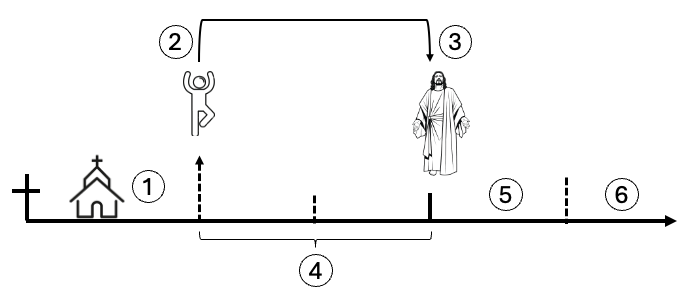
\includegraphics[
    width=1\textwidth,
    trim=0 0 0 0,
    clip]{images/pretribulation.png}
    \caption{The Pretribulation Rapture }
    \label{fig:pretribulation}
\end{figure}
The sequence of events in the pretribulation\index{Rapture!pretribulation view} view is illustrated in Figure~\ref{fig:pretribulation}: 
\begin{itemize}
\item[\ding{172} ] the Church Age; 
\item[\ding{173} ] the Rapture\index{Rapture} before the Great Tribulation\index{Great Tribulation};
\item[\ding{174} ] Christ's return to earth with His people to reign; 
\item[\ding{175} ] the Great Tribulation; 
\item[\ding{176} ] the Millennium\index{millennium}; 
\item[\ding{177} ] the new heaven and the new earth.
\end{itemize}



\section*{The Midtribulation Rapture}\index{Rapture!midtribulation view}\index{Rapture}

The midtribulation\index{Rapture!midtribulation view} view holds that the church will pass through the first three and a half years of the Great Tribulation\index{Great Tribulation} and then be caught up before God's wrath\index{wrath of God} is poured out in the latter half. Its proponents regard the midpoint of Daniel\index{Daniel}'s seventieth seven as a decisive turning point and connect the ``last trumpet'' mentioned by Paul with the seventh trumpet\index{trumpets, seven!7@seventh trumpet} in Revelation.

The principal passages cited in support of this view include the following:

\begin{itemize}
\item \textbf{Daniel 9:27:} In the middle of the seven, sacrifice and offering will cease. The midpoint of the seven-year period is therefore understood as a major dividing line in the prophetic sequence.
\item \textbf{1 Corinthians 15:52:} Paul says that believers will be changed at the last trumpet. Advocates of the midtribulation\index{Rapture!midtribulation view} view identify this trumpet with the seventh trumpet\index{trumpets, seven!7@seventh trumpet} in Revelation 11:15.
\item \textbf{Revelation 11:11--12:} After the two witnesses\index{two witnesses} have prophesied for 1,260 days\index{1,260 days}, they hear a voice from heaven calling, ``Come up here.'' They ascend to heaven in a cloud. Some interpreters regard this scene as a picture of the Rapture\index{Rapture} taking place in the middle of the Tribulation.
\item \textbf{Revelation 11:15, 18:} When the seventh angel sounds his trumpet, heaven announces that God's kingdom has come and that His wrath has arrived. Advocates of this view place the outpouring of divine wrath, particularly the seven bowls\index{bowls, seven} described in Revelation 16, in the latter half of the Tribulation.
\item \textbf{1 Thessalonians 5:9:} God has not appointed believers to suffer wrath. Midtribulation interpreters distinguish the persecution\index{persecution} inflicted by human powers and the Antichrist\index{Antichrist} during the first half from the outpouring of God's wrath during the second half. They therefore conclude that believers will be caught up before that wrath begins.
\item \textbf{2 Thessalonians 2:3--4:} Before the gathering of believers, the man of lawlessness must be revealed and exalt himself in the temple\index{temple} of God, proclaiming himself to be God. This is commonly associated by advocates of this view with the midpoint of the seven-year period and with the abomination of desolation mentioned in Matthew 24\index{Matthew 24}:15.
\end{itemize}

\begin{figure}[htbp]
    \centering
    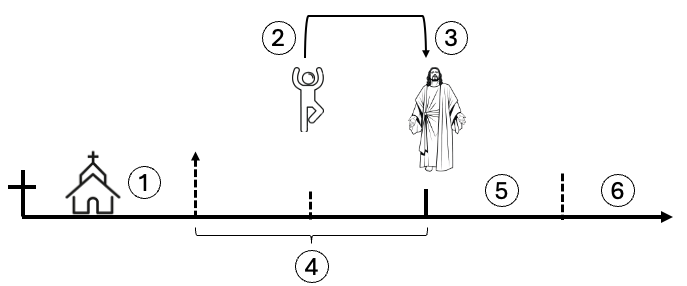
\includegraphics[
    width=1\textwidth,
    trim=0 0 0 0,
    clip]{images/midtribulation.png}
    \caption{The Midtribulation Rapture }
    \label{fig:midtribulation}
\end{figure}


The sequence of events in the midtribulation\index{Rapture!midtribulation view} view is illustrated in Figure~\ref{fig:midtribulation}: 
\begin{itemize}
\item[\ding{172} ] the Church Age; 
\item[\ding{173} ] the Rapture\index{Rapture} during the Great Tribulation\index{Great Tribulation};
\item[\ding{174} ] Christ's return to earth with His people to reign;
\item[\ding{175} ] the Great Tribulation; 
\item[\ding{176} ] the Millennium\index{millennium};
\item[\ding{177} ] the new heaven and the new earth.
\end{itemize}


\section*{The Posttribulation Rapture}\index{Rapture!posttribulation view}\index{Rapture}

The posttribulation\index{Rapture!posttribulation view} view holds that the church will pass through the Great Tribulation\index{Great Tribulation}. Believers will be caught up to meet the Lord in the air when Christ returns in glory\index{glory} at the end of that period. Proponents argue that the New Testament places the gathering of God's people after the Tribulation.

The principal passages cited in support of this view include the following:

\begin{itemize}
\item \textbf{Matthew 24\index{Matthew 24}:29--31:} Jesus says that immediately after the distress of those days, the Son of Man\index{Son of Man} will appear and send His angels with a loud trumpet call to gather His elect from the four winds. Advocates of the posttribulation\index{Rapture!posttribulation view} view understand this as clear evidence that the gathering of God's people takes place after the Tribulation.
\item \textbf{2 Thessalonians 2:1--3:} Paul speaks of the coming of the Lord Jesus Christ and the gathering of believers to Him. He then explains that the day will not come until the rebellion occurs and the man of lawlessness is revealed. This is understood to mean that the Antichrist\index{Antichrist} will appear before believers are gathered to the Lord.
\item \textbf{2 Thessalonians 1:6--7:} Paul assures those suffering persecution\index{persecution} that they will receive relief when the Lord Jesus is revealed from heaven with His mighty angels. Advocates of this view understand this relief as coming at Christ's public return in glory.
\item \textbf{1 Corinthians 15:52:} Paul's reference to the last trumpet is understood in connection with the trumpet call in Matthew 24:31, suggesting that the transformation and gathering of believers occur at Christ's visible return.
\item \textbf{Revelation 20:4--5:} Those who bore witness to Jesus and refused to worship\index{worship} the beast\index{beast} come to life in what John calls ``the first resurrection\index{first resurrection}.'' Interpreters who understand this resurrection as occurring after the Great Tribulation\index{Great Tribulation} conclude that the resurrection of believers, and thus the Rapture\index{Rapture}, takes place after the Tribulation as well.
\item \textbf{John 17:15:} Jesus does not ask the Father to take His disciples out of the world, but to protect them from the evil one. Advocates of the posttribulation view see here a pattern of divine preservation: God can guard His people through times of suffering without necessarily removing them from those circumstances.
\end{itemize}

Advocates of this view also point to Old Testament events that illustrate God's ability to preserve His people through judgment rather than remove them beforehand:

\begin{itemize}
\item \textbf{Genesis 7:1, 23:} Noah was not taken away before the Flood. Instead, he passed through it in the ark and was preserved by God.
\item \textbf{Exodus 8:22:} When God brought plagues\index{plagues} upon Egypt\index{Egypt}, the Israelites remained in the land, but God set apart the region of Goshen so that the plague would not fall upon His people there.
\end{itemize}


\begin{figure}[htbp]
    \centering
    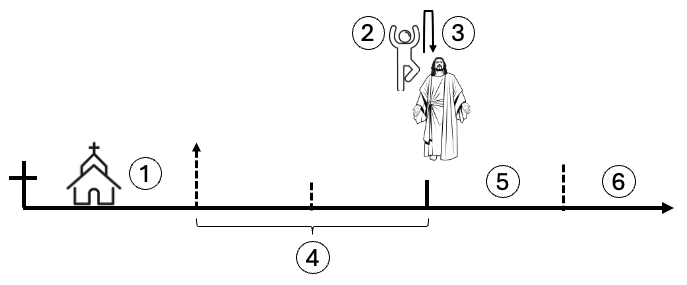
\includegraphics[
    width=1\textwidth,
    trim=0 0 0 0,
    clip]{images/posttribulation.png}
    \caption{The Posttribulation Rapture}
    \label{fig:posttribulation}
\end{figure}

The sequence of events in the posttribulation\index{Rapture!posttribulation view} view is illustrated in Figure~\ref{fig:posttribulation}: 
\begin{itemize}
\item[\ding{172} ] the Church Age; 
\item[\ding{173} ] the Rapture\index{Rapture} after the Great Tribulation\index{Great Tribulation}; 
\item[\ding{174} ] Christ's return to earth with His people to reign; 
\item[\ding{175} ] the Great Tribulation; 
\item[\ding{176} ] the Millennium\index{millennium}; 
\item[\ding{177} ] the new heaven and the new earth.
\end{itemize}


%\appendix
\refstepcounter{chapter} 
\chapter*{Views of the Millennium} 
\markboth{Appendix~\thechapter\quad Views of the Millennium}%
         {Appendix~\thechapter\quad Views of the Millennium}
%\addcontentsline{toc}{chapter} {\protect\numberline{Appendix~\thechapter} Views of the Millennium}
\addcontentsline{toc}{chapter} {\protect\numberline{\thechapter} Views of the Millennium}





When we seek to understand the Millennium described in Revelation, three principal interpretations emerge: premillennialism, postmillennialism, and amillennialism. Each offers a different way of understanding the relationship between Christ's return, the Millennium, and the coming of the new heaven and the new earth. Figures~\ref{fig:premillennialism}, \ref{fig:postmillennialism}, and \ref{fig:amillennialism} provide a visual guide to these three views.

\section*{Premillennialism}

\begin{figure}[htbp]
    \centering
    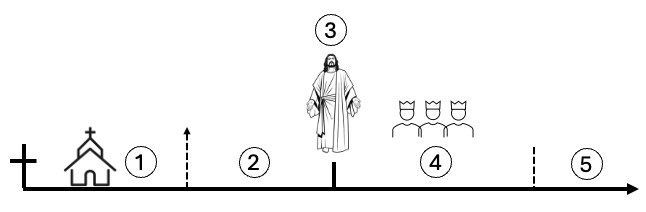
\includegraphics[width=\textwidth]{images/premillennialism.png}
    \caption{Premillennialism}
    \label{fig:premillennialism}
\end{figure}

According to the premillennial view, the sequence is:

\begin{itemize}
\item[\ding{172} ] the Church Age, 
\item[\ding{173} ] a period of great tribulation. 
\item[\ding{174} ] Jesus Christ returns. 
\item[\ding{175} ] the Millennium starts and the saints reign with Christ. 
\item[\ding{176} ] God brings forth the new heaven and the new earth.
\end{itemize}



\section*{Postmillennialism}

According to the postmillennial view, the sequence begins with \ding{172} the Church Age, followed by \ding{173} the Millennium. After this period, \ding{174} Jesus Christ returns, and finally \ding{175} God brings forth the new heaven and the new earth.

\begin{figure}[htbp]
    \centering
    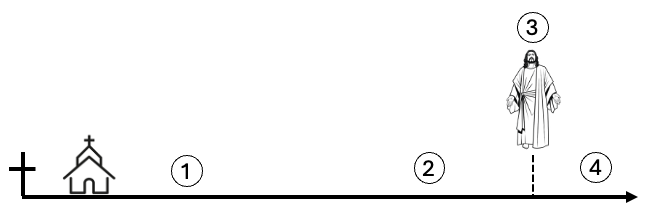
\includegraphics[width=\textwidth]{images/postmillennialism.png}
    \caption{Postmillennialism}
    \label{fig:postmillennialism}
\end{figure}

\section*{Amillennialism}

According to the amillennial view, \ding{172} the present Church Age is itself the Millennium. The thousand years are understood symbolically, representing Christ's present reign rather than a separate, future thousand-year kingdom on earth. At the close of this age, \ding{173} Jesus Christ returns, and \ding{174} God brings forth the new heaven and the new earth.

\begin{figure}[htbp]
    \centering
    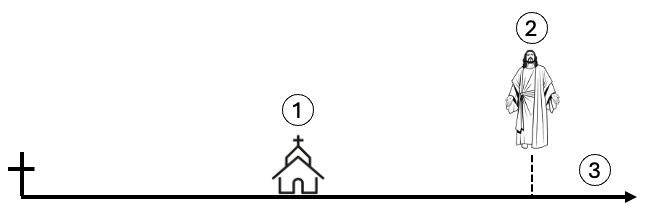
\includegraphics[width=\textwidth]{images/amillennialism.png}
    \caption{Amillennialism}
    \label{fig:amillennialism}
\end{figure}

\begingroup
\small
\renewcommand{\arraystretch}{1.1}
\begin{longtable}{
  >{\RaggedRight\arraybackslash}p{0.15\linewidth}
  >{\RaggedRight\arraybackslash}p{0.24\linewidth}
  >{\RaggedRight\arraybackslash}p{0.24\linewidth}
  >{\RaggedRight\arraybackslash}p{0.24\linewidth}}
\caption{A Comparison of the Three Views of the Millennium}
\label{tab:millennium}\\
\hline
\textbf{Topic} & \textbf{Premil.}\footnote{Representative proponents of premillennialism include Justin Martyr, Irenaeus, Tertullian, John F. Walvoord, and Charles Ryrie.} & \textbf{Postmil.}\footnote{Representative proponents of postmillennialism include Jonathan Edwards, Charles Hodge, and R. C. Sproul.} & \textbf{Amil.}\footnote{Representative proponents of amillennialism include Augustine, John Calvin, and G. K. Beale.} \\
\hline
\endfirsthead

\multicolumn{4}{l}{\footnotesize\itshape Table~\thetable\ (continued)}\\
\hline
\textbf{Topic} & \textbf{Premil.} & \textbf{Postmil.} & \textbf{Amil.} \\
\hline
\endhead

\hline
\multicolumn{4}{r}{\footnotesize\itshape Continued on next page}\\
\endfoot

\hline
\endlastfoot

Christ's return &
Before the Millennium &
After the Millennium &
After the Millennium, understood as the Church Age \\

The Millennium &
A literal thousand-year reign of Christ on earth following His return &
A period in which the gospel advances powerfully throughout the world, bringing widespread conversion, righteousness, and peace; generally understood symbolically rather than as a literal thousand years &
The Church Age, represented by a symbolic thousand years, during which Christ reigns now in heaven \\

Satan's binding &
Released for a short time at the end of the thousand years, then thrown into the lake of fire &
Greatly restrained so that he cannot prevent the gospel from reaching the nations; his binding is understood to occur before or during the Millennium &
Restrained from preventing the gospel from reaching the nations, though he remains active in opposing God's people \\

The resurrection &
Two stages: believers are raised before or at the beginning of the Millennium; unbelievers are raised afterward for judgment &
A general resurrection of both believers and unbelievers at Christ's return &
As in postmillennialism: a general resurrection of both believers and unbelievers at Christ's return \\

The final rebellion &
After the Millennium &
Near the end of the Millennium &
At the close of the present age \\
\end{longtable}
\endgroup
\refstepcounter{chapter} 
\chapter*{Teacher's Guide} 
\markboth{Appendix~\thechapter\quad Teacher's Guide}%
         {Appendix~\thechapter\quad Teacher's Guide}
%\addcontentsline{toc}{chapter} {\protect\numberline{Appendix~\thechapter} A Guide for Teachers}
\addcontentsline{toc}{chapter} {\protect\numberline{\thechapter} Teacher's Guide}




This book is suitable for adult Sunday school classes and small-group Bible studies. The following schedules are designed to help teachers and group leaders plan their sessions. I recommend the 8-week plan for a regular Sunday school course, while retaining the ten-week plan as an option for more in-depth study.

\section*{(1) 6 Weeks}

This plan is suitable for groups with limited time who wish to grasp the central message of the entire book in six weeks. Each session covers one or more related chapters, focusing on the identity of Christ, redemption, judgment, victory, and the new creation.

{
\small
\renewcommand{\arraystretch}{1}

\begin{longtable}{
  >{\centering\arraybackslash}p{0.5cm}
  >{\raggedright\arraybackslash}p{0.8cm}
  >{\raggedright\arraybackslash}p{1.6cm}
  >{\raggedright\arraybackslash}p{5.8cm}
}

\textbf{Wk} &
\textbf{Ch.} &
\textbf{Revelation} &
\textbf{Focus} \\
\hline
\endfirsthead

\textbf{Wk} &
\textbf{Ch.} &
\textbf{Revelation} &
\textbf{Focus} \\
\hline
\endhead

\textbf{1} &
1--2 &
1--3 &
Explore Christ's commendations, rebukes, commands, and promises to the seven churches. \\

\textbf{2} &
3--4 &
4--5 &
Discover why Christ alone is worthy to open the scroll and how history rests under His sovereign rule. \\

\textbf{3} &
4--5 &
6--7 &
Study the seven seals, the four horsemen, the cry of the martyrs, the sealed servants of God, and the worship of a multitude from every nation.  \\

\textbf{4} &
5--6 &
8--11 &
Explore the judgments of the seven trumpets, the two witnesses, and the seventh trumpet. \\

\textbf{5} &
7--10 &
12--19 &
Examine the dragon, the beasts, the false prophet, and Babylon as manifestations of powers opposed to God.  \\

\textbf{6} &
11--12 &
20--22 &
Explore the different views of the Millennium, the final judgment, the new heaven and the new earth, and the New Jerusalem.  \\
\hline
\end{longtable}

}

\section*{(2) 8 Weeks}

This is the plan I recommend most highly. Each session can last approximately 60--75 minutes, allowing time both to introduce the major visions of Revelation and to discuss church life, faithful witness amid suffering, differing views of the end times, and the Christian's ultimate hope.





{ \small \renewcommand{\arraystretch}{1} \begin{longtable}{ >{\centering\arraybackslash}p{0.5cm} >{\raggedright\arraybackslash}p{0.8cm} >{\raggedright\arraybackslash}p{2cm} >{\raggedright\arraybackslash}p{5.4cm} } \textbf{Wk} & \textbf{Ch.} & \textbf{Revelation} & \textbf{Focus} \\ \hline \endfirsthead \textbf{Wk} & \textbf{Ch.} & \textbf{Revelation} & \textbf{Focus} \\ \hline \endhead \textbf{1} & 1 & 1:1--20 & Explore the background of John and his exile on Patmos. Through Christ's suffering, resurrection, and reign, discover the central figure of Revelation. \\ \textbf{2} & 2 & 2:1--3:22 & Study the commendations, rebukes, commands, and promises given to the seven churches.  \\ \textbf{3} & 3 & 4:1--5:14 & Move from the Lord who created all things to the Lamb who was slain.  \\ \textbf{4} & 4 & 6:1--7:17 & Study the seven seals, the four horsemen, the martyrs, the sealed servants of God, and the worship of a multitude from every nation.  \\ \textbf{5} & 5--6 & 8:1--11:19 & Study the seven trumpets, the two witnesses, and the seventh trumpet. \\ \textbf{6} & 7 & 12:1--14:20 & Explore the symbolism of the woman, the male child, the dragon, the beast from the sea, and the false prophet. \\ \textbf{7} & 8--10 & 15:1--19:21 & Study the seven bowls, the fall of Babylon, the wedding supper of the Lamb, and Christ riding on the white horse. \\ \textbf{8} & 11--12 & 20:1--22:21 & Study the Millennium, the final judgment, the new heaven and the new earth, and the New Jerusalem.  \\ \hline \end{longtable} 
}


\section*{(3) 10 Weeks}

The 10-week plan makes the fullest use of this book's distinctive features. It is particularly suitable for Sunday school teacher training, adult Bible study groups, and readers who wish to gain a deeper understanding of the symbols in Revelation and the different interpretations of the end times.

{ \small \renewcommand{\arraystretch}{1} \begin{longtable}{ >{\centering\arraybackslash}p{0.5cm} >{\raggedright\arraybackslash}p{0.8cm} >{\raggedright\arraybackslash}p{2cm} >{\raggedright\arraybackslash}p{5.4cm} } \textbf{Wk} & \textbf{Ch.} & \textbf{Revelation} & \textbf{Focus} \\ \hline \endfirsthead \textbf{Wk} & \textbf{Ch.} & \textbf{Revelation} & \textbf{Focus} \\ \hline \endhead \textbf{1} & 1 & 1:1--20 & Explore the background of Revelation, John's witness, and the identity of Christ as the One who passed through suffering into glory. \\ \textbf{2} & 2 & 2:1--3:22 & Examine each of the seven churches, comparing their circumstances, strengths, weaknesses, and promises. \\ \textbf{3} & 3 & 4:1--5:14 & Study the heavenly throne, the four living creatures, the twenty-four elders, and the Lamb. \\ \textbf{4} & 4 & 6:1--7:17 & Study the seven seals, the four horsemen, the cry of the martyrs, the 144,000 who are sealed, and the multitude from every nation. \\ \textbf{5} & 5 & 8:1--9:21 & Study the first six trumpets and their accompanying visions. \\ \textbf{6} & 6 & 10:1--11:19 & Study the little scroll, the two witnesses, and the seventh trumpet. \\ \textbf{7} & 7 & 12:1--14:20 & Examine the woman, the male child, the dragon, the two beasts, and the 144,000. \\ \textbf{8} & 8--10 & 15:1--19:21 & Study the seven bowls, the fall of Babylon, the wedding supper of the Lamb, and Christ's return. \\ \textbf{9} & 11 & 20:1--15 & Study Satan's binding, the Millennium, Gog and Magog, and the great white throne. \\ \textbf{10} & 12 & 21:1--22:21 & Study the New Jerusalem, God's dwelling with His people, the river of life, and the tree of life. \\ \hline \end{longtable} 

}


\clearpage
\printindex

\end{document}